\documentclass[mathserif]{beamer}
\usepackage[utf8]{inputenc}
\usepackage{amsmath}
\usepackage{amsfonts}
\usepackage{amssymb}
\usepackage{arydshln}
\usepackage{graphicx}
\usepackage{float}
\usepackage{picture}
\usepackage{dcolumn}
\usepackage{textpos}
\usepackage{graphicx}
\usepackage{subcaption}
\usepackage{tikz}
\usepackage{pgfplots}
\usepackage{listings}
\usepackage{minted}
\setminted{
	framesep=2mm,
	bgcolor=black!5,
	fontsize=\footnotesize,
	linenos,
	obeytabs,
	tabsize=4,
	mathescape = true,
	escapeinside=@@
}


\setbeamercolor{structure}{fg=grey}
\usetheme[sectionpage=progressbar, progressbar=frametitle]{metropolis}

\definecolor{prettyBlue}{HTML}{2196F3}
\setbeamercolor{progress bar}{fg=prettyBlue, bg=gray}

%Information to be included in the title page:
\title{Development of a Pendulum Control System}
\author{Thomas S. Christensen \\ Mikkel S. Jaedicke\\}

\institute{University of Southern Denmark}
\date{Jan, 2018} 

\addtobeamertemplate{frametitle}{}{%
\begin{textblock*}{200mm}(\textwidth-1.5cm,-0.8cm)
\includegraphics[scale=0.15]{graphics/sdu_logo}
\end{textblock*}}

\begin{document}

\begin{frame}[t]\frametitle{~}
\maketitle
\end{frame}

\begin{frame}[c]\frametitle{Introduction}
\includegraphics[width=\textwidth]{graphics/workflow}
\vfill
	\begin{columns}
		\begin{column}[c]{.5\textwidth}
			\begin{itemize}
				\item \alert<1>{Analysis}
				\item \alert<2>{Design}
			\end{itemize}
		\end{column}
		\begin{column}[c]{.5\textwidth}
			\begin{itemize}
				\item \alert<3>{Implementation}
				\item \alert<4>{Verification}
			\end{itemize}
		\end{column}
	\end{columns}
	\vspace{0.5cm}
	\hrule
	\vspace{0.4cm}
	
	\begin{columns}
		\begin{column}[c]{.5\textwidth}
			\begin{itemize}
				\item<5> \alert<5>{Conclusion}
			\end{itemize}
		\end{column}
		\begin{column}[c]{.5\textwidth}
			\begin{itemize}
				\item[~]
			\end{itemize}
		\end{column}
	\end{columns}
\end{frame}

\section{Analysis}

\begin{frame}[c]\frametitle{Analysis\\ A Platform for Teaching Underactuated Systems}
	\begin{columns}
		\begin{column}[c]{.5\textwidth}
			\begin{itemize}[<+- | alert@+>]
				\item What is an underactuated system?
				\item Pendulum systems.
				\item Double pendulum system.
			\end{itemize}
		\end{column}
		\begin{column}[c]{.5\textwidth}
			\centering
			\includegraphics<1>[width=\linewidth]{graphics/robo_underactuated}\\
			\vspace{1cm}
			\includegraphics<1>[width=.50\linewidth]{graphics/robo_underactuated_picture}
			\includegraphics<2>[width=\linewidth]{graphics/segway}
			\includegraphics<3>[width=\linewidth]{graphics/joint_assembly.eps}
		\end{column}
	\end{columns}
\end{frame}

\begin{frame}[c]\frametitle{System Overview}
\centering
\includegraphics[scale=1]{graphics/system_overview}
\end{frame}

\begin{frame}[c]\frametitle{Implemented System}
\centering
\includegraphics[width=0.9\textwidth]{graphics/full_system_finish}
\end{frame}

\begin{frame}[c]\frametitle{Requirement Specification}

\textbf{Functional:}
\begin{enumerate}
	\item System should consists of a double pendulum mounted on a moveable cart.
	\item Cart should be actuated by the Maxon 148867. 
	\item The pendulum system should be controlled by a MicroZed.
	\item \alert<2>{Position of the cart and joint angles should be measured.}
\end{enumerate}

\end{frame}

\section{Design}

\begin{frame}{Mechanical Design}
	\begin{figure}
	\centering
	\begin{subfigure}{.5\textwidth}
	  \centering
	  \includegraphics[width=.9\linewidth]{graphics/joint_read_side}
	\end{subfigure}%
	\begin{subfigure}{.5\textwidth}
	  \centering
	  \includegraphics[width=.9\linewidth]{graphics/joint_mag_assembly}
	\end{subfigure}
	\end{figure}
\end{frame}

\begin{frame}[c]\frametitle{Electrical Design}
	\begin{itemize}
    	\item Encoder
    	\item Wireless Communication
    	\item Microcontroller
    	\item Power Delivery
    \end{itemize}    
\end{frame}

\begin{frame}[c]\frametitle{Electrical Design}
	\begin{itemize}
    	\item Encoder
    	\item Wireless Communication
    	\item Microcontroller
    	\item \alert{Power Delivery}
    \end{itemize}    
\end{frame}

\begin{frame}[c]\frametitle{Power Delivery}
	\centering
	\vfill
    \includegraphics[width=.35\linewidth]{graphics/lipo}\\
    \vfill
    \scalebox{2}{$$3.0V\;\rightarrow\;4.2V \quad\Rightarrow\quad 3.3V$$}
    \vfill
\end{frame}

\begin{frame}[c]{Test Columns}
\begin{columns}
\column{.5\linewidth}
\textbf{Solutions:}   
\begin{itemize}
			\item Buck converter
			\item Buck-Boost converter
			\item Linear regulator
\end{itemize}
\column{.5\linewidth}
\textbf{Parameters:}
\begin{itemize}
			\item Efficiency
			\item Drop out voltage
			\item []
\end{itemize}
\end{columns}
\end{frame}

\begin{frame}[c]\frametitle{Buck Converter}
	\begin{equation}
		V_{drop} = I_{O} \cdot (R_{DS(on)}+R_I)
		\label{eq:drop_v_tps62}
	\end{equation}

	\begin{equation}
		V_{drop} = 0.02 \cdot (0.062+0.09) = 14 [mV]
		\label{eq:drop_v_tps62_2}
	\end{equation}

	\begin{equation}
		\eta \approx 95\%
	\end{equation}
\end{frame}

\begin{frame}[c]\frametitle{Comparison}
	\begin{table}[h]
		\begin{tabular}{l|c|c|c}
			  ~				& \textbf{Buck} 	& \textbf{Buck-Boost}& \textbf{Linear}\tabularnewline 
			 Efficiency  	& 95\% 	& 75\%		& 89\%	\\
			 Drop out [mV]	& 14  	& N/A		& 20	\\
		\end{tabular}
	\end{table}
\end{frame}

\begin{frame}[t]\frametitle{Battery Characteristics}
    \begin{figure}[h]
		\centering
		%% This file was created by matlab2tikz.
%
%The latest updates can be retrieved from
%  http://www.mathworks.com/matlabcentral/fileexchange/22022-matlab2tikz-matlab2tikz
%where you can also make suggestions and rate matlab2tikz.
%
\definecolor{mycolor1}{rgb}{0.00000,0.44700,0.74100}%
%
\begin{tikzpicture}

\begin{axis}[%
width=0.951\fwidth,
height=\fheight,
at={(0\fwidth,0\fheight)},
scale only axis,
xmin=0,
xmax=450,
xlabel style={font=\color{white!15!black}},
xlabel={Time [Min]},
ymin=2.5,
ymax=4.5,
ytick={2.5, 2.7, 2.9, 3.1, 3.3, 3.5, 3.7, 3.9, 4.1, 4.3, 4.5},
ylabel style={font=\color{white!15!black}},
ylabel={Voltage [V]},
axis background/.style={fill=white},
title style={font=\bfseries},
title={Discharge Curve of Battery}
]
\addplot [color=mycolor1, forget plot]
  table[row sep=crcr]{%
0	4.072\\
10	4.02699999999999\\
20	4.00799999999998\\
40	3.95999999999998\\
50	3.92200000000003\\
60	3.89499999999998\\
70	3.87900000000002\\
80	3.85500000000002\\
90	3.84300000000002\\
100	3.81799999999998\\
110	3.79700000000003\\
120	3.78899999999999\\
130	3.77699999999999\\
140	3.767\\
150	3.75299999999999\\
160	3.76100000000002\\
170	3.75999999999999\\
180	3.74000000000001\\
190	3.72500000000002\\
200	3.71300000000002\\
210	3.714\\
220	3.69999999999999\\
230	3.71100000000001\\
240	3.71199999999999\\
250	3.69999999999999\\
260	3.69299999999998\\
270	3.69099999999997\\
280	3.69799999999998\\
290	3.69099999999997\\
300	3.68099999999998\\
310	3.673\\
320	3.65699999999998\\
330	3.64499999999998\\
340	3.63499999999999\\
350	3.62299999999999\\
360	3.60700000000003\\
370	3.61399999999998\\
380	3.596\\
390	3.56799999999998\\
400	3.505\\
410	3.36099999999999\\
414.551694551695	2.30000000000001\\
};
\addplot [color=red, dashed, forget plot]
  table[row sep=crcr]{%
0	3.30000000000001\\
450	3.30000000000001\\
};
\end{axis}
\end{tikzpicture}%
	\end{figure}
\end{frame}

\begin{frame}[c]\frametitle{Designed PCB}
	\begin{figure}
	\centering
	\includegraphics[width=.7\linewidth]{graphics/joint_assembly}
	\end{figure}
\end{frame}

\begin{frame}[c]\frametitle{Designed Pendulum Assembly}
	\begin{figure}
	\centering
	\includegraphics[width=.32\linewidth]{graphics/pendulum_assembly}
	\end{figure}
\end{frame}

\begin{frame}{Software Design}
	\begin{figure}
	\centering
	  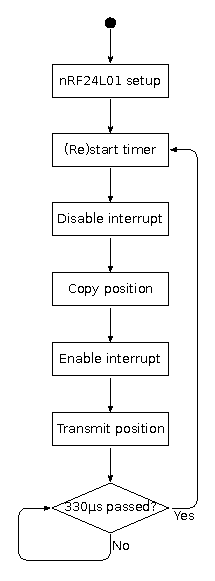
\includegraphics[width=.25\linewidth]{graphics/joint_software_diagram}
	\end{figure}
\end{frame}

%\begin{frame}{Software Design}
%	\begin{figure}
%	\centering
%	  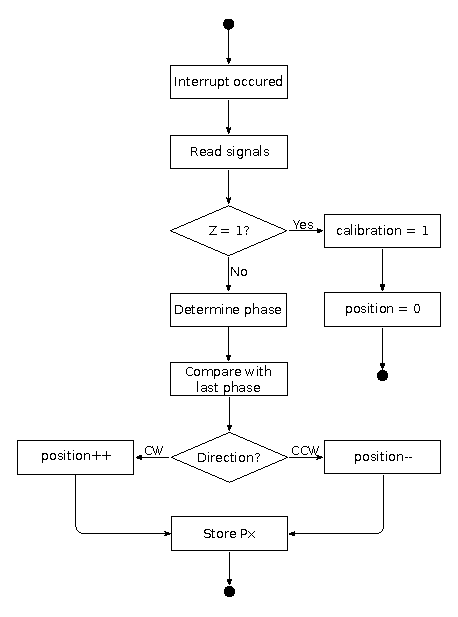
\includegraphics[width=.55\linewidth]{graphics/joint_interrupt}
%	\end{figure}
%\end{frame}



\section{Implementation}

\begin{frame}[c]\frametitle{Implementation of Joint Board PCB}
\begin{figure}
	\centering
	\begin{subfigure}{.5\textwidth}
	  \centering
	  \includegraphics[width=.9\linewidth]{graphics/joint_board_pic}
	\end{subfigure}%
	\begin{subfigure}{.5\textwidth}
	  \centering
	  \includegraphics[width=.9\linewidth]{graphics/joint_board_pop_pic}
	\end{subfigure}
	\end{figure}
\end{frame}

\begin{frame}[c]\frametitle{Implementation of Full System}
	\begin{figure}
		\centering
		\includegraphics[width=.9\linewidth]{graphics/full_system_finish_high}
	\end{figure}
\end{frame}

\begin{frame}[c]\frametitle{Implementation Pendulum Assembly}
	\begin{figure}
		\centering
		\includegraphics[width=.4\linewidth]{graphics/joint_ass_real}
	\end{figure}
\end{frame}


\section{Verification}



\begin{frame}[c]\frametitle{TEST - SINGLE PENDULUM}
   	\begin{figure}
		\centering
		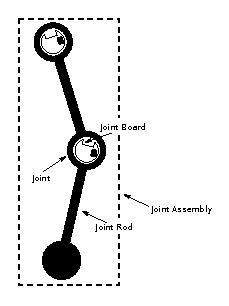
\includegraphics[width=.7\linewidth]{graphics/joint_assembly.eps}
	\end{figure} 
\end{frame}

\begin{frame}[c]\frametitle{.....}
    \begin{figure}[h]
		\centering
		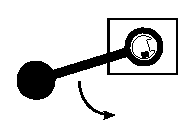
\includegraphics[width=.5\linewidth]{graphics/single_pendulum}
	\end{figure}
\end{frame}

\begin{frame}[c]\frametitle{.....}
    \begin{figure}[h]
		\centering
		\input{graphics/joint_angle_measured_full_sine.tex}
	\end{figure}
\end{frame}

\begin{frame}[c]\frametitle{.....}
    \begin{figure}[h]
		\centering
		%% This file was created by matlab2tikz.
%
%The latest updates can be retrieved from
%  http://www.mathworks.com/matlabcentral/fileexchange/22022-matlab2tikz-matlab2tikz
%where you can also make suggestions and rate matlab2tikz.
%
\definecolor{mycolor1}{rgb}{0.00000,0.44700,0.74100}%
%
\begin{tikzpicture}

\begin{axis}[%
width=.9\textwidth,
height=2.5in,
at={(0.758in,0.481in)},
scale only axis,
xmin=3000,
xmax=4400,
xlabel style={font=\color{white!15!black}},
xlabel={Time [us]},
ymin=2500,
ymax=7000,
ylabel style={font=\color{white!15!black}},
ylabel={Angle [ticks]},
axis background/.style={fill=white},
title style={font=\bfseries},
title={Joint Angle Transmission},
axis x line*=bottom,
axis y line*=left
]
\addplot[only marks, mark=*, mark options={}, mark size=0.5000pt, draw=mycolor1] table[row sep=crcr]{%
x	y\\
2989	6326\\
2990	6331\\
2991	6337\\
2993	6348\\
2994	6353\\
2995	6358\\
2996	6363\\
2997	6368\\
2998	6373\\
2999	6377\\
3000	6382\\
3001	6387\\
3003	6396\\
3004	6401\\
3006	6410\\
3008	6418\\
3010	6426\\
3011	6430\\
3013	6438\\
3014	6442\\
3016	6450\\
3017	6453\\
3020	6464\\
3021	6467\\
3023	6474\\
3026	6483\\
3027	6486\\
3028	6489\\
3029	6492\\
3030	6495\\
3031	6497\\
3032	6500\\
3033	6503\\
3034	6505\\
3035	6508\\
3036	6510\\
3037	6513\\
3039	6517\\
3040	6519\\
3041	6521\\
3042	6523\\
3043	6525\\
3044	6527\\
3045	6529\\
3046	6531\\
3047	6533\\
3048	6534\\
3050	6538\\
3051	6539\\
3052	6541\\
3053	6542\\
3056	6546\\
3059	6549\\
3060	6550\\
3061	6551\\
3062	6552\\
3063	6553\\
3065	6554\\
3066	6555\\
3068	6556\\
3070	6556\\
3071	6557\\
3073	6557\\
3075	6558\\
3076	6558\\
3078	6558\\
3079	6557\\
3080	6557\\
3081	6557\\
3082	6557\\
3083	6556\\
3084	6556\\
3085	6555\\
3086	6555\\
3087	6554\\
3088	6554\\
3090	6552\\
3091	6551\\
3092	6551\\
3094	6549\\
3096	6546\\
3098	6544\\
3099	6543\\
3100	6541\\
3101	6540\\
3102	6538\\
3103	6537\\
3105	6534\\
3106	6532\\
3109	6526\\
3110	6524\\
3112	6520\\
3113	6518\\
3115	6514\\
3116	6511\\
3118	6507\\
3119	6504\\
3120	6501\\
3121	6499\\
3122	6496\\
3123	6493\\
3124	6490\\
3126	6484\\
3127	6481\\
3129	6475\\
3130	6472\\
3132	6465\\
3134	6459\\
3136	6451\\
3137	6448\\
3138	6444\\
3140	6436\\
3141	6432\\
3144	6420\\
3146	6412\\
3147	6407\\
3149	6398\\
3150	6394\\
3151	6389\\
3154	6375\\
3156	6365\\
3157	6360\\
3158	6355\\
3160	6345\\
3161	6339\\
3162	6334\\
3164	6323\\
3165	6318\\
3166	6312\\
3167	6307\\
3168	6301\\
3172	6277\\
3174	6265\\
3175	6258\\
3176	6252\\
3178	6239\\
3181	6219\\
3182	6212\\
3183	6205\\
3184	6198\\
3185	6191\\
3188	6169\\
3189	6162\\
3190	6154\\
3191	6147\\
3192	6139\\
3193	6131\\
3194	6123\\
3195	6115\\
3196	6107\\
3197	6099\\
3198	6091\\
3199	6083\\
3201	6066\\
3202	6058\\
3204	6041\\
3206	6023\\
3207	6014\\
3208	6006\\
3209	5996\\
3210	5987\\
3213	5960\\
3214	5951\\
3215	5941\\
3216	5931\\
3217	5922\\
3218	5912\\
3220	5892\\
3221	5882\\
3222	5873\\
3223	5863\\
3224	5853\\
3225	5842\\
3226	5832\\
3227	5821\\
3229	5800\\
3231	5779\\
3233	5758\\
3234	5747\\
3235	5735\\
3236	5724\\
3237	5713\\
3238	5702\\
3239	5691\\
3240	5679\\
3241	5668\\
3242	5657\\
3243	5645\\
3244	5633\\
3245	5621\\
3247	5598\\
3248	5586\\
3250	5562\\
3251	5550\\
3252	5537\\
3256	5488\\
3257	5475\\
3258	5463\\
3259	5450\\
3260	5437\\
3261	5424\\
3262	5411\\
3263	5398\\
3264	5385\\
3265	5372\\
3266	5359\\
3267	5346\\
3268	5333\\
3269	5319\\
3270	5306\\
3271	5292\\
3272	5279\\
3274	5252\\
3275	5238\\
3276	5224\\
3277	5210\\
3278	5196\\
3279	5183\\
3280	5169\\
3281	5155\\
3285	5098\\
3287	5070\\
3288	5056\\
3289	5041\\
3290	5027\\
3291	5012\\
3295	4955\\
3296	4940\\
3297	4925\\
3298	4911\\
3299	4896\\
3300	4882\\
3301	4867\\
3302	4852\\
3303	4837\\
3306	4793\\
3307	4778\\
3309	4749\\
3310	4734\\
3311	4719\\
3312	4704\\
3313	4689\\
3314	4674\\
3315	4659\\
3316	4644\\
3318	4614\\
3320	4584\\
3321	4570\\
3322	4555\\
3323	4540\\
3324	4525\\
3325	4510\\
3328	4465\\
3329	4450\\
3330	4435\\
3332	4405\\
3333	4390\\
3334	4376\\
3335	4361\\
3336	4346\\
3337	4332\\
3338	4317\\
3339	4302\\
3341	4273\\
3342	4258\\
3343	4244\\
3344	4229\\
3345	4214\\
3346	4200\\
3347	4185\\
3348	4171\\
3351	4129\\
3352	4114\\
3353	4100\\
3354	4086\\
3355	4072\\
3356	4058\\
3357	4044\\
3358	4030\\
3359	4017\\
3360	4003\\
3361	3987\\
3362	3973\\
3364	3945\\
3365	3932\\
3367	3904\\
3368	3890\\
3369	3877\\
3370	3864\\
3371	3851\\
3372	3838\\
3374	3811\\
3375	3798\\
3376	3785\\
3377	3772\\
3378	3760\\
3379	3747\\
3380	3734\\
3382	3709\\
3383	3697\\
3384	3684\\
3385	3672\\
3386	3660\\
3387	3647\\
3389	3623\\
3391	3599\\
3392	3587\\
3393	3575\\
3394	3564\\
3395	3552\\
3396	3541\\
3397	3529\\
3398	3518\\
3399	3506\\
3401	3484\\
3402	3473\\
3403	3462\\
3404	3451\\
3405	3440\\
3406	3429\\
3408	3408\\
3409	3397\\
3410	3387\\
3411	3376\\
3412	3366\\
3413	3356\\
3414	3346\\
3417	3316\\
3418	3306\\
3419	3296\\
3420	3286\\
3422	3267\\
3423	3258\\
3424	3248\\
3428	3212\\
3429	3203\\
3430	3194\\
3431	3185\\
3432	3176\\
3433	3167\\
3435	3150\\
3436	3142\\
3437	3134\\
3440	3109\\
3441	3101\\
3442	3093\\
3443	3085\\
3445	3069\\
3446	3062\\
3447	3054\\
3448	3047\\
3449	3039\\
3450	3032\\
3451	3024\\
3452	3017\\
3453	3010\\
3454	3003\\
3456	2989\\
3457	2982\\
3458	2976\\
3459	2969\\
3461	2956\\
3462	2950\\
3463	2943\\
3464	2937\\
3465	2931\\
3469	2907\\
3470	2901\\
3471	2895\\
3472	2889\\
3473	2884\\
3475	2873\\
3477	2862\\
3478	2857\\
3479	2852\\
3480	2847\\
3481	2842\\
3483	2832\\
3484	2827\\
3485	2822\\
3486	2817\\
3487	2813\\
3489	2804\\
3490	2799\\
3492	2791\\
3493	2787\\
3494	2782\\
3496	2775\\
3497	2771\\
3498	2767\\
3499	2763\\
3500	2759\\
3501	2756\\
3502	2752\\
3505	2742\\
3506	2739\\
3508	2732\\
3509	2729\\
3510	2726\\
3511	2723\\
3512	2720\\
3513	2717\\
3515	2712\\
3516	2709\\
3518	2704\\
3520	2699\\
3521	2697\\
3522	2695\\
3524	2690\\
3525	2688\\
3526	2686\\
3527	2684\\
3529	2681\\
3530	2679\\
3531	2677\\
3532	2676\\
3540	2665\\
3541	2664\\
3542	2663\\
3547	2659\\
3548	2658\\
3550	2657\\
3551	2656\\
3552	2656\\
3553	2655\\
3554	2655\\
3555	2655\\
3556	2655\\
3557	2655\\
3558	2654\\
3559	2654\\
3560	2654\\
3561	2654\\
3562	2655\\
3564	2655\\
3565	2655\\
3566	2656\\
3567	2656\\
3569	2657\\
3570	2658\\
3571	2658\\
3572	2659\\
3574	2661\\
3575	2662\\
3576	2663\\
3577	2664\\
3578	2665\\
3580	2667\\
3581	2668\\
3583	2671\\
3584	2672\\
3586	2675\\
3587	2677\\
3588	2679\\
3589	2680\\
3590	2682\\
3591	2684\\
3592	2686\\
3593	2688\\
3594	2690\\
3595	2692\\
3596	2694\\
3597	2697\\
3598	2699\\
3600	2704\\
3601	2706\\
3602	2709\\
3604	2714\\
3605	2717\\
3607	2723\\
3608	2726\\
3611	2735\\
3612	2738\\
3613	2742\\
3614	2745\\
3615	2748\\
3618	2759\\
3619	2762\\
3620	2766\\
3621	2770\\
3622	2774\\
3625	2786\\
3626	2790\\
3627	2794\\
3628	2799\\
3629	2803\\
3630	2807\\
3631	2812\\
3632	2816\\
3634	2826\\
3635	2831\\
3636	2836\\
3637	2840\\
3639	2851\\
3640	2856\\
3641	2861\\
3643	2871\\
3644	2877\\
3645	2882\\
3646	2888\\
3647	2893\\
3648	2899\\
3649	2905\\
3650	2911\\
3651	2917\\
3654	2935\\
3655	2941\\
3656	2948\\
3658	2960\\
3660	2973\\
3661	2980\\
3662	2987\\
3663	2994\\
3666	3015\\
3667	3022\\
3670	3044\\
3672	3059\\
3674	3074\\
3675	3082\\
3676	3089\\
3680	3122\\
3681	3130\\
3682	3138\\
3685	3163\\
3686	3172\\
3687	3181\\
3688	3189\\
3689	3198\\
3690	3207\\
3692	3225\\
3695	3253\\
3696	3262\\
3697	3272\\
3698	3281\\
3701	3310\\
3702	3320\\
3703	3330\\
3704	3340\\
3705	3350\\
3706	3360\\
3707	3370\\
3709	3391\\
3710	3401\\
3711	3412\\
3712	3422\\
3713	3433\\
3715	3455\\
3716	3465\\
3717	3476\\
3719	3499\\
3720	3510\\
3721	3521\\
3722	3532\\
3723	3544\\
3724	3555\\
3725	3567\\
3726	3578\\
3727	3590\\
3729	3614\\
3730	3626\\
3731	3638\\
3732	3650\\
3733	3662\\
3734	3674\\
3735	3686\\
3736	3698\\
3737	3711\\
3738	3723\\
3739	3736\\
3740	3749\\
3741	3761\\
3742	3774\\
3743	3786\\
3745	3812\\
3746	3825\\
3747	3838\\
3748	3851\\
3749	3864\\
3750	3877\\
3751	3891\\
3752	3904\\
3753	3917\\
3754	3931\\
3756	3958\\
3757	3972\\
3758	3986\\
3759	4002\\
3760	4015\\
3761	4029\\
3762	4043\\
3763	4057\\
3764	4070\\
3765	4084\\
3766	4098\\
3767	4112\\
3768	4126\\
3769	4140\\
3770	4154\\
3771	4168\\
3773	4196\\
3774	4211\\
3776	4239\\
3779	4283\\
3780	4297\\
3782	4326\\
3783	4341\\
3786	4384\\
3787	4399\\
3788	4413\\
3789	4428\\
3791	4458\\
3792	4472\\
3793	4487\\
3794	4502\\
3795	4516\\
3797	4546\\
3798	4561\\
3799	4575\\
3800	4590\\
3801	4605\\
3802	4619\\
3803	4634\\
3804	4649\\
3805	4663\\
3806	4678\\
3807	4693\\
3808	4707\\
3809	4722\\
3810	4737\\
3811	4751\\
3812	4766\\
3813	4781\\
3814	4795\\
3815	4810\\
3817	4839\\
3818	4854\\
3819	4868\\
3820	4882\\
3821	4897\\
3822	4911\\
3823	4925\\
3824	4940\\
3825	4954\\
3826	4968\\
3827	4982\\
3828	4997\\
3829	5011\\
3830	5025\\
3831	5039\\
3832	5053\\
3833	5067\\
3834	5081\\
3835	5095\\
3836	5109\\
3837	5123\\
3838	5137\\
3839	5151\\
3844	5219\\
3845	5232\\
3846	5246\\
3847	5259\\
3848	5272\\
3849	5285\\
3851	5312\\
3852	5325\\
3853	5338\\
3854	5351\\
3855	5364\\
3856	5377\\
3857	5389\\
3858	5402\\
3859	5415\\
3860	5427\\
3861	5440\\
3863	5465\\
3864	5477\\
3865	5489\\
3866	5501\\
3868	5526\\
3869	5538\\
3870	5550\\
3874	5596\\
3875	5608\\
3876	5620\\
3877	5631\\
3878	5642\\
3881	5676\\
3882	5687\\
3883	5698\\
3884	5709\\
3885	5720\\
3886	5731\\
3887	5741\\
3888	5752\\
3889	5763\\
3890	5773\\
3892	5793\\
3893	5804\\
3894	5814\\
3896	5834\\
3897	5844\\
3899	5864\\
3900	5874\\
3901	5883\\
3902	5892\\
3903	5902\\
3904	5912\\
3905	5921\\
3908	5949\\
3909	5958\\
3911	5975\\
3912	5984\\
3913	5993\\
3914	6001\\
3915	6010\\
3917	6027\\
3918	6035\\
3919	6043\\
3920	6052\\
3921	6060\\
3922	6068\\
3923	6076\\
3924	6083\\
3925	6091\\
3926	6099\\
3927	6107\\
3928	6114\\
3929	6122\\
3930	6129\\
3931	6136\\
3932	6144\\
3933	6151\\
3935	6165\\
3936	6172\\
3937	6179\\
3938	6185\\
3939	6192\\
3942	6212\\
3945	6231\\
3948	6249\\
3949	6255\\
3950	6261\\
3952	6272\\
3953	6278\\
3954	6283\\
3956	6294\\
3957	6299\\
3959	6310\\
3960	6315\\
3961	6320\\
3962	6325\\
3963	6330\\
3964	6334\\
3966	6344\\
3967	6349\\
3968	6353\\
3969	6358\\
3970	6362\\
3971	6367\\
3972	6371\\
3973	6375\\
3974	6379\\
3976	6387\\
3977	6391\\
3979	6399\\
3980	6403\\
3982	6410\\
3983	6414\\
3984	6417\\
3985	6421\\
3986	6424\\
3987	6427\\
3988	6431\\
3989	6434\\
3990	6437\\
3991	6440\\
3992	6443\\
3993	6446\\
3995	6452\\
3997	6457\\
3998	6460\\
3999	6462\\
4000	6465\\
4001	6467\\
4002	6469\\
4004	6474\\
4005	6476\\
4007	6480\\
4008	6482\\
4011	6487\\
4012	6489\\
4013	6491\\
4014	6492\\
4015	6494\\
4016	6496\\
4017	6497\\
4019	6500\\
4020	6501\\
4022	6503\\
4023	6505\\
4025	6506\\
4027	6508\\
4028	6509\\
4030	6510\\
4032	6512\\
4033	6512\\
4034	6512\\
4035	6513\\
4036	6513\\
4037	6513\\
4038	6514\\
4039	6514\\
4041	6514\\
4042	6514\\
4043	6514\\
4044	6514\\
4046	6513\\
4047	6513\\
4051	6511\\
4052	6510\\
4053	6510\\
4054	6509\\
4055	6508\\
4057	6507\\
4058	6506\\
4060	6504\\
4061	6502\\
4062	6501\\
4063	6500\\
4064	6499\\
4065	6497\\
4066	6496\\
4067	6494\\
4069	6491\\
4070	6489\\
4071	6488\\
4072	6486\\
4075	6480\\
4076	6478\\
4077	6476\\
4078	6474\\
4079	6472\\
4080	6470\\
4081	6467\\
4082	6465\\
4083	6462\\
4084	6460\\
4085	6457\\
4086	6455\\
4087	6452\\
4088	6449\\
4089	6446\\
4091	6440\\
4094	6431\\
4095	6428\\
4096	6424\\
4097	6421\\
4098	6418\\
4099	6414\\
4100	6411\\
4101	6407\\
4102	6403\\
4103	6399\\
4104	6395\\
4105	6391\\
4106	6387\\
4108	6380\\
4109	6375\\
4110	6371\\
4112	6363\\
4113	6359\\
4114	6354\\
4115	6349\\
4116	6345\\
4118	6335\\
4120	6326\\
4121	6321\\
4122	6316\\
4123	6311\\
4124	6306\\
4125	6300\\
4126	6295\\
4127	6289\\
4128	6284\\
4129	6279\\
4130	6273\\
4131	6268\\
4132	6262\\
4134	6250\\
4135	6244\\
4136	6238\\
4137	6232\\
4139	6219\\
4140	6213\\
4141	6207\\
4143	6193\\
4144	6187\\
4145	6180\\
4146	6173\\
4147	6166\\
4149	6152\\
4150	6145\\
4151	6138\\
4152	6131\\
4155	6108\\
4156	6101\\
4159	6077\\
4160	6069\\
4161	6061\\
4163	6045\\
4166	6020\\
4167	6012\\
4168	6003\\
4169	5995\\
4170	5986\\
4171	5977\\
4172	5968\\
4173	5960\\
4174	5951\\
4175	5941\\
4176	5932\\
4177	5923\\
4178	5914\\
4182	5876\\
4183	5866\\
4184	5857\\
4188	5817\\
4189	5807\\
4190	5796\\
4191	5786\\
4192	5776\\
4193	5765\\
4194	5755\\
4195	5744\\
4196	5733\\
4197	5723\\
4198	5712\\
4199	5701\\
4200	5690\\
4201	5679\\
4202	5668\\
4203	5657\\
4204	5646\\
4205	5634\\
4206	5623\\
4207	5612\\
4210	5577\\
4211	5565\\
4213	5541\\
4214	5529\\
4215	5517\\
4216	5505\\
4217	5493\\
4218	5481\\
4219	5469\\
4221	5444\\
4222	5431\\
4223	5419\\
4224	5406\\
4226	5381\\
4227	5368\\
4228	5355\\
4231	5316\\
4232	5303\\
4233	5290\\
4234	5277\\
4235	5264\\
4237	5237\\
4238	5223\\
4239	5210\\
4241	5183\\
4242	5169\\
4243	5156\\
4244	5142\\
4245	5128\\
4246	5114\\
4247	5100\\
4248	5086\\
4249	5073\\
4250	5059\\
4251	5045\\
4252	5031\\
4253	5016\\
4254	5002\\
4255	4988\\
4256	4974\\
4257	4960\\
4260	4917\\
4261	4903\\
4263	4874\\
4264	4860\\
4265	4845\\
4266	4831\\
4267	4816\\
4268	4802\\
4269	4787\\
4270	4773\\
4271	4758\\
4272	4744\\
4273	4729\\
4274	4714\\
4275	4700\\
4276	4685\\
4277	4671\\
4278	4656\\
4279	4642\\
4280	4627\\
4281	4612\\
4282	4598\\
4283	4583\\
4285	4554\\
4286	4539\\
4287	4525\\
4288	4510\\
4289	4495\\
4290	4481\\
4291	4466\\
4292	4452\\
4294	4422\\
4295	4408\\
4296	4393\\
4297	4379\\
4298	4364\\
4299	4350\\
4300	4335\\
4303	4292\\
4304	4278\\
4305	4264\\
4306	4249\\
4307	4235\\
4308	4221\\
4309	4207\\
4310	4192\\
4311	4178\\
4312	4165\\
4313	4151\\
4314	4137\\
4315	4123\\
4316	4109\\
4317	4095\\
4318	4081\\
4319	4068\\
4320	4054\\
4321	4040\\
4322	4027\\
4323	4013\\
4324	3998\\
4325	3984\\
4326	3971\\
4327	3957\\
4328	3944\\
4329	3931\\
4330	3917\\
4331	3903\\
4332	3890\\
4333	3877\\
4334	3864\\
4335	3852\\
4336	3839\\
4337	3826\\
4338	3813\\
4339	3800\\
4340	3787\\
4341	3775\\
4342	3763\\
4343	3750\\
4344	3738\\
4346	3713\\
4347	3701\\
4348	3689\\
4349	3677\\
4350	3665\\
4351	3653\\
4352	3641\\
4353	3630\\
4354	3618\\
4355	3606\\
4356	3594\\
4357	3583\\
4358	3572\\
4360	3549\\
4361	3538\\
4362	3527\\
4363	3516\\
4364	3505\\
4365	3494\\
4366	3483\\
4367	3473\\
4368	3462\\
4369	3451\\
4371	3430\\
4372	3420\\
4373	3410\\
4375	3389\\
4378	3359\\
4379	3350\\
4380	3340\\
4381	3330\\
4382	3321\\
4383	3311\\
4384	3302\\
4385	3292\\
4386	3283\\
4387	3274\\
4388	3265\\
4389	3256\\
4390	3247\\
4391	3238\\
4392	3229\\
4393	3220\\
4395	3203\\
4397	3186\\
4398	3178\\
4400	3161\\
4401	3153\\
4402	3145\\
4403	3137\\
4404	3129\\
4405	3121\\
4408	3098\\
4409	3091\\
4410	3083\\
4411	3076\\
4412	3069\\
4413	3061\\
4414	3054\\
4415	3047\\
4416	3040\\
4418	3027\\
4419	3020\\
4420	3013\\
4421	3007\\
4423	2994\\
4424	2987\\
4425	2981\\
4427	2969\\
4428	2963\\
4429	2957\\
4431	2945\\
4432	2939\\
4433	2933\\
4435	2922\\
4436	2917\\
4439	2901\\
4440	2895\\
4441	2890\\
4443	2880\\
4444	2875\\
4445	2871\\
4446	2866\\
4447	2861\\
4448	2857\\
4450	2848\\
4451	2843\\
4454	2830\\
4455	2826\\
4456	2822\\
4458	2814\\
4459	2810\\
4461	2803\\
4462	2799\\
4463	2796\\
4465	2789\\
4466	2785\\
4468	2779\\
4469	2776\\
4472	2766\\
4474	2761\\
4475	2758\\
4476	2755\\
4477	2753\\
4478	2750\\
4479	2748\\
4481	2743\\
4483	2738\\
4484	2736\\
4486	2732\\
4487	2730\\
4488	2728\\
4490	2724\\
4495	2716\\
4496	2714\\
4497	2713\\
4499	2710\\
4501	2708\\
4502	2707\\
4503	2706\\
4504	2705\\
4505	2704\\
4507	2702\\
4508	2701\\
4510	2700\\
4511	2700\\
4512	2699\\
4513	2699\\
4514	2698\\
4516	2698\\
4518	2697\\
4519	2697\\
4520	2697\\
4521	2697\\
4522	2697\\
4523	2697\\
4524	2697\\
4525	2698\\
4527	2698\\
4528	2699\\
4529	2699\\
4530	2700\\
4533	2702\\
4534	2703\\
4535	2703\\
4537	2705\\
4538	2706\\
4539	2707\\
4541	2710\\
4542	2711\\
4544	2714\\
4545	2715\\
4547	2718\\
4548	2720\\
4550	2723\\
4551	2725\\
4553	2729\\
4557	2737\\
4558	2740\\
4559	2742\\
4560	2744\\
4561	2747\\
4562	2749\\
4563	2752\\
4564	2754\\
4565	2757\\
4566	2760\\
4567	2763\\
4569	2768\\
4570	2771\\
4571	2775\\
4572	2778\\
4573	2781\\
4576	2791\\
4577	2794\\
4578	2798\\
4579	2802\\
4580	2805\\
4581	2809\\
4583	2817\\
4584	2821\\
4585	2825\\
4586	2829\\
4587	2833\\
4588	2837\\
4589	2842\\
4590	2846\\
4591	2850\\
4592	2855\\
4593	2859\\
4594	2864\\
4595	2869\\
4596	2874\\
4597	2878\\
4598	2883\\
4601	2898\\
4602	2904\\
4604	2914\\
4605	2920\\
4606	2925\\
4607	2931\\
4608	2937\\
4610	2948\\
4611	2954\\
4612	2960\\
4613	2966\\
4614	2972\\
4620	3010\\
4621	3016\\
4622	3023\\
4624	3037\\
4625	3044\\
4626	3051\\
4628	3065\\
4629	3072\\
4630	3079\\
4631	3087\\
4633	3102\\
4634	3109\\
4636	3125\\
4638	3140\\
4639	3148\\
4640	3156\\
4643	3181\\
4644	3189\\
4645	3198\\
4646	3206\\
4648	3223\\
4649	3232\\
4650	3241\\
4651	3250\\
4652	3259\\
4653	3268\\
4654	3277\\
4655	3286\\
4657	3304\\
4658	3314\\
4659	3323\\
4661	3342\\
4662	3352\\
4663	3362\\
4664	3372\\
4665	3382\\
4666	3392\\
4667	3402\\
4669	3422\\
4670	3433\\
4671	3443\\
4672	3453\\
4674	3474\\
4675	3485\\
4676	3496\\
4677	3507\\
4682	3562\\
4684	3584\\
4685	3596\\
4687	3619\\
4688	3631\\
4689	3642\\
4690	3654\\
4696	3726\\
4697	3738\\
4699	3762\\
4700	3775\\
4701	3787\\
4702	3799\\
4703	3812\\
4704	3825\\
4705	3838\\
4707	3863\\
4708	3876\\
4709	3889\\
4711	3915\\
4712	3928\\
4713	3942\\
4714	3955\\
4715	3968\\
4716	3982\\
4717	3995\\
4718	4010\\
4719	4024\\
4720	4037\\
4722	4064\\
4724	4091\\
4725	4105\\
4726	4118\\
4728	4146\\
4729	4160\\
4731	4187\\
4733	4215\\
4734	4229\\
4735	4243\\
4736	4258\\
4738	4286\\
4740	4314\\
4741	4328\\
4742	4343\\
4747	4414\\
4748	4428\\
4749	4443\\
4750	4457\\
4752	4486\\
4753	4500\\
4754	4515\\
4755	4529\\
4756	4544\\
4757	4558\\
4758	4573\\
4760	4601\\
4761	4616\\
4762	4630\\
4763	4645\\
4764	4659\\
4765	4673\\
4767	4702\\
4768	4716\\
4769	4731\\
4770	4745\\
4771	4760\\
4772	4774\\
4773	4788\\
4774	4802\\
4775	4817\\
4776	4831\\
4780	4887\\
4781	4902\\
4782	4916\\
4784	4944\\
4785	4958\\
4787	4985\\
4789	5013\\
4790	5027\\
4793	5069\\
4794	5082\\
4796	5110\\
4797	5123\\
4798	5137\\
4799	5150\\
4800	5164\\
4801	5177\\
4802	5190\\
4803	5203\\
4804	5217\\
4805	5230\\
4806	5243\\
4808	5269\\
4809	5282\\
4810	5295\\
4811	5308\\
4813	5333\\
4814	5346\\
4815	5359\\
4818	5396\\
4819	5408\\
4821	5433\\
4823	5458\\
4824	5469\\
4825	5481\\
4826	5493\\
4827	5505\\
4828	5517\\
4829	5529\\
4830	5540\\
4831	5552\\
4832	5563\\
4833	5575\\
4834	5586\\
4835	5597\\
4838	5631\\
4839	5642\\
4840	5653\\
4841	5664\\
4842	5675\\
4843	5685\\
4844	5696\\
4847	5727\\
4848	5738\\
4849	5748\\
4850	5758\\
4851	5768\\
4853	5788\\
4855	5808\\
4857	5828\\
4858	5837\\
4859	5847\\
4860	5857\\
4861	5866\\
4863	5884\\
4864	5893\\
4865	5903\\
4866	5912\\
4868	5930\\
4869	5938\\
4870	5947\\
4872	5964\\
4874	5981\\
4875	5989\\
4876	5998\\
4877	6006\\
4878	6014\\
4879	6022\\
4880	6030\\
4881	6038\\
4882	6046\\
4883	6054\\
4884	6061\\
4885	6069\\
4886	6076\\
4888	6091\\
4889	6098\\
4890	6105\\
4891	6113\\
4892	6120\\
4894	6134\\
4896	6147\\
4897	6154\\
4898	6160\\
4899	6167\\
4900	6173\\
4903	6192\\
4904	6198\\
4905	6204\\
4907	6216\\
4908	6222\\
4911	6239\\
4912	6245\\
4913	6250\\
4914	6256\\
4915	6261\\
4919	6281\\
4921	6291\\
4922	6296\\
4923	6300\\
4924	6305\\
4926	6314\\
4927	6319\\
4929	6327\\
4932	6340\\
4933	6344\\
4934	6348\\
4935	6352\\
4936	6356\\
4937	6360\\
4938	6363\\
4939	6367\\
4940	6370\\
4941	6374\\
4942	6377\\
4943	6381\\
4944	6384\\
4945	6387\\
4946	6390\\
4948	6397\\
4949	6400\\
4950	6403\\
4951	6406\\
4952	6408\\
4953	6411\\
4954	6414\\
4955	6416\\
4960	6429\\
4961	6431\\
4962	6433\\
4964	6437\\
4965	6439\\
4967	6443\\
4968	6445\\
4970	6449\\
4971	6450\\
4972	6452\\
4974	6455\\
4975	6456\\
};
\end{axis}
\end{tikzpicture}%
	\end{figure}
\end{frame}

\begin{frame}[c]\frametitle{.....}
    \begin{figure}[h]
		\centering
		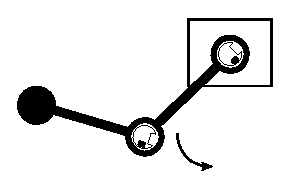
\includegraphics[width=.75\linewidth]{graphics/double_pendulum}
	\end{figure}
\end{frame}

\begin{frame}[c]\frametitle{.....}
    \begin{figure}[h]
		\centering
		% This file was created by matlab2tikz.
%
%The latest updates can be retrieved from
%  http://www.mathworks.com/matlabcentral/fileexchange/22022-matlab2tikz-matlab2tikz
%where you can also make suggestions and rate matlab2tikz.
%
\definecolor{mycolor1}{rgb}{0.00000,0.44700,0.74100}%
%
\begin{tikzpicture}

\begin{axis}[%
width=.8\textwidth,
height=2in,
at={(0.758in,0.481in)},
scale only axis,
xmin=66000,
xmax=90000,
xlabel style={font=\color{white!15!black}},
xlabel={Time [us]},
ymin=3000,
ymax=6500,
ylabel style={font=\color{white!15!black}},
ylabel={Angle [ticks]},
axis background/.style={fill=white},
title style={font=\bfseries},
title={Joint Angle},
axis x line*=bottom,
axis y line*=left
]
\addplot[only marks, mark=*, mark options={}, mark size=0.5000pt, draw=mycolor1] table[row sep=crcr]{%
x	y\\
56874	4676\\
56877	4600\\
56879	4600\\
56881	4600\\
56882	4600\\
56884	4600\\
56885	4600\\
56887	4600\\
56888	4600\\
56889	4600\\
56890	4600\\
56891	4600\\
56893	4600\\
56894	4600\\
56895	4600\\
56897	4600\\
56899	4600\\
56900	4600\\
56901	4600\\
56902	4600\\
56903	4600\\
56905	4600\\
56907	4600\\
56908	4600\\
56912	4600\\
56913	4600\\
56915	4600\\
56916	4600\\
56917	4600\\
56918	4600\\
56919	4600\\
56921	4600\\
56922	4600\\
56924	4600\\
56927	4600\\
56928	4600\\
56930	4600\\
56931	4600\\
56936	4600\\
56938	4600\\
56939	4600\\
56940	4600\\
56941	4600\\
56943	4600\\
56944	4600\\
56945	4600\\
56946	4600\\
56947	4600\\
56948	4600\\
56949	4600\\
56950	4600\\
56951	4600\\
56952	4600\\
56953	4600\\
56954	4600\\
56956	4600\\
56957	4600\\
56958	4600\\
56959	4600\\
56960	4600\\
56961	4600\\
56963	4600\\
56964	4600\\
56966	4600\\
56967	4600\\
56968	4600\\
56969	4600\\
56971	4600\\
56972	4600\\
56973	4600\\
56974	4600\\
56975	4600\\
56977	4600\\
56978	4600\\
56980	4600\\
56981	4600\\
56983	4600\\
56984	4600\\
56985	4600\\
56986	4600\\
56987	4600\\
56988	4600\\
56989	4600\\
56990	4600\\
56991	4600\\
56992	4600\\
56993	4600\\
56995	4600\\
56997	4600\\
56998	4600\\
56999	4600\\
57000	4600\\
57002	4600\\
57003	4600\\
57005	4600\\
57006	4600\\
57009	4600\\
57010	4600\\
57011	4600\\
57012	4600\\
57013	4600\\
57014	4600\\
57015	4600\\
57016	4600\\
57017	4600\\
57019	4600\\
57020	4600\\
57022	4600\\
57023	4600\\
57025	4600\\
57026	4600\\
57029	4600\\
57030	4600\\
57031	4600\\
57032	4600\\
57033	4600\\
57034	4600\\
57035	4600\\
57036	4600\\
57037	4600\\
57038	4600\\
57039	4600\\
57040	4600\\
57041	4600\\
57042	4600\\
57043	4600\\
57044	4600\\
57045	4600\\
57046	4600\\
57047	4600\\
57048	4600\\
57050	4600\\
57051	4600\\
57052	4600\\
57053	4600\\
57054	4600\\
57056	4600\\
57057	4600\\
57058	4600\\
57060	4600\\
57062	4600\\
57063	4600\\
57064	4600\\
57065	4600\\
57066	4600\\
57067	4600\\
57068	4600\\
57069	4600\\
57070	4600\\
57072	4600\\
57074	4600\\
57075	4600\\
57076	4600\\
57077	4600\\
57078	4600\\
57080	4600\\
57081	4600\\
57082	4600\\
57083	4600\\
57084	4600\\
57085	4600\\
57086	4600\\
57087	4600\\
57090	4600\\
57091	4600\\
57093	4600\\
57094	4600\\
57095	4600\\
57096	4600\\
57097	4600\\
57098	4600\\
57101	4600\\
57102	4600\\
57104	4600\\
57105	4600\\
57106	4600\\
57107	4600\\
57108	4600\\
57109	4600\\
57110	4600\\
57111	4600\\
57112	4600\\
57113	4600\\
57114	4600\\
57115	4600\\
57116	4600\\
57119	4600\\
57121	4600\\
57122	4600\\
57124	4600\\
57125	4600\\
57127	4600\\
57129	4600\\
57131	4600\\
57132	4600\\
57133	4600\\
57134	4600\\
57135	4600\\
57136	4600\\
57137	4600\\
57138	4600\\
57139	4600\\
57140	4600\\
57141	4600\\
57145	4600\\
57146	4600\\
57147	4600\\
57148	4600\\
57149	4600\\
57151	4600\\
57152	4600\\
57153	4600\\
57154	4600\\
57155	4600\\
57156	4600\\
57160	4600\\
57161	4600\\
57162	4600\\
57163	4600\\
57164	4600\\
57166	4600\\
57167	4600\\
57168	4600\\
57169	4600\\
57171	4600\\
57172	4600\\
57174	4600\\
57176	4600\\
57177	4600\\
57179	4600\\
57180	4600\\
57182	4600\\
57183	4600\\
57185	4600\\
57186	4600\\
57188	4600\\
57189	4600\\
57190	4600\\
57191	4600\\
57193	4600\\
57194	4600\\
57195	4600\\
57196	4600\\
57197	4600\\
57198	4600\\
57199	4600\\
57200	4600\\
57201	4600\\
57203	4600\\
57204	4600\\
57205	4600\\
57209	4600\\
57210	4600\\
57211	4600\\
57212	4600\\
57213	4600\\
57214	4600\\
57215	4600\\
57216	4600\\
57217	4600\\
57219	4600\\
57220	4600\\
57222	4600\\
57223	4600\\
57224	4600\\
57226	4600\\
57227	4600\\
57228	4600\\
57229	4600\\
57231	4600\\
57234	4600\\
57236	4600\\
57238	4600\\
57239	4600\\
57240	4600\\
57241	4600\\
57242	4600\\
57243	4600\\
57244	4600\\
57245	4600\\
57246	4600\\
57247	4600\\
57248	4600\\
57249	4600\\
57251	4600\\
57252	4600\\
57253	4600\\
57254	4600\\
57256	4600\\
57257	4600\\
57259	4600\\
57260	4600\\
57261	4600\\
57262	4600\\
57264	4600\\
57265	4600\\
57267	4600\\
57268	4600\\
57269	4600\\
57270	4600\\
57271	4600\\
57272	4600\\
57273	4600\\
57275	4600\\
57276	4600\\
57277	4600\\
57278	4600\\
57279	4600\\
57280	4600\\
57281	4600\\
57282	4600\\
57283	4600\\
57284	4600\\
57285	4600\\
57287	4600\\
57289	4600\\
57292	4600\\
57293	4600\\
57294	4600\\
57295	4600\\
57296	4600\\
57298	4600\\
57300	4600\\
57301	4600\\
57303	4600\\
57304	4600\\
57306	4600\\
57307	4600\\
57308	4600\\
57309	4600\\
57311	4600\\
57312	4600\\
57314	4600\\
57316	4600\\
57319	4600\\
57321	4600\\
57322	4600\\
57323	4600\\
57324	4600\\
57325	4600\\
57326	4600\\
57328	4600\\
57329	4600\\
57330	4600\\
57331	4600\\
57332	4600\\
57333	4600\\
57334	4600\\
57335	4600\\
57336	4600\\
57337	4600\\
57338	4600\\
57339	4600\\
57340	4600\\
57341	4600\\
57342	4600\\
57343	4600\\
57344	4600\\
57345	4600\\
57346	4600\\
57347	4600\\
57348	4600\\
57349	4600\\
57350	4600\\
57351	4600\\
57352	4600\\
57354	4600\\
57355	4600\\
57356	4600\\
57357	4600\\
57358	4600\\
57360	4600\\
57361	4600\\
57362	4600\\
57363	4600\\
57366	4600\\
57367	4600\\
57368	4600\\
57369	4600\\
57370	4600\\
57373	4600\\
57374	4600\\
57375	4600\\
57376	4600\\
57377	4600\\
57378	4600\\
57380	4600\\
57382	4600\\
57383	4600\\
57384	4600\\
57386	4600\\
57388	4600\\
57389	4600\\
57390	4600\\
57391	4600\\
57392	4600\\
57393	4600\\
57394	4600\\
57396	4600\\
57400	4600\\
57401	4600\\
57403	4600\\
57404	4600\\
57405	4600\\
57406	4600\\
57407	4600\\
57408	4600\\
57409	4600\\
57410	4600\\
57411	4600\\
57412	4600\\
57413	4600\\
57414	4600\\
57415	4600\\
57416	4600\\
57417	4600\\
57418	4600\\
57419	4600\\
57420	4600\\
57422	4600\\
57423	4600\\
57425	4600\\
57427	4600\\
57428	4600\\
57430	4600\\
57431	4600\\
57432	4600\\
57433	4600\\
57434	4600\\
57435	4600\\
57436	4600\\
57437	4600\\
57438	4600\\
57439	4600\\
57440	4600\\
57441	4600\\
57442	4600\\
57443	4600\\
57444	4600\\
57445	4600\\
57446	4600\\
57447	4600\\
57448	4600\\
57449	4600\\
57450	4600\\
57451	4600\\
57453	4600\\
57454	4600\\
57455	4600\\
57456	4600\\
57457	4600\\
57459	4600\\
57460	4600\\
57461	4600\\
57462	4600\\
57463	4600\\
57465	4600\\
57466	4600\\
57467	4600\\
57468	4600\\
57469	4600\\
57471	4600\\
57472	4600\\
57473	4600\\
57474	4600\\
57475	4600\\
57476	4600\\
57477	4600\\
57478	4600\\
57479	4600\\
57480	4600\\
57483	4600\\
57484	4600\\
57485	4600\\
57486	4600\\
57488	4600\\
57489	4600\\
57490	4600\\
57491	4600\\
57492	4600\\
57494	4600\\
57495	4600\\
57496	4600\\
57497	4600\\
57498	4600\\
57500	4600\\
57501	4600\\
57502	4600\\
57503	4600\\
57506	4600\\
57507	4600\\
57508	4600\\
57509	4600\\
57510	4600\\
57511	4600\\
57512	4600\\
57513	4600\\
57514	4600\\
57515	4600\\
57517	4600\\
57518	4600\\
57519	4600\\
57520	4600\\
57521	4600\\
57523	4600\\
57524	4600\\
57525	4600\\
57526	4600\\
57527	4600\\
57528	4600\\
57529	4600\\
57530	4600\\
57531	4600\\
57532	4600\\
57535	4600\\
57536	4600\\
57537	4600\\
57538	4600\\
57540	4600\\
57541	4600\\
57542	4600\\
57543	4600\\
57544	4600\\
57545	4600\\
57546	4600\\
57547	4600\\
57548	4600\\
57549	4600\\
57550	4600\\
57552	4600\\
57553	4600\\
57554	4600\\
57555	4600\\
57556	4600\\
57557	4600\\
57558	4600\\
57559	4600\\
57560	4600\\
57561	4600\\
57564	4600\\
57565	4600\\
57566	4600\\
57567	4600\\
57568	4600\\
57569	4600\\
57570	4600\\
57571	4600\\
57572	4600\\
57574	4600\\
57575	4600\\
57576	4600\\
57577	4600\\
57578	4600\\
57581	4600\\
57582	4600\\
57583	4600\\
57584	4600\\
57587	4600\\
57588	4600\\
57589	4600\\
57590	4600\\
57592	4600\\
57593	4600\\
57594	4600\\
57595	4600\\
57596	4600\\
57598	4600\\
57599	4600\\
57600	4600\\
57601	4600\\
57602	4600\\
57604	4600\\
57605	4600\\
57606	4600\\
57607	4600\\
57608	4600\\
57610	4600\\
57611	4600\\
57612	4600\\
57613	4600\\
57614	4600\\
57616	4600\\
57617	4600\\
57618	4600\\
57619	4600\\
57621	4600\\
57622	4600\\
57623	4600\\
57624	4600\\
57625	4600\\
57627	4600\\
57628	4600\\
57629	4600\\
57630	4600\\
57631	4600\\
57633	4600\\
57634	4600\\
57635	4600\\
57636	4600\\
57637	4600\\
57639	4600\\
57640	4600\\
57641	4600\\
57642	4600\\
57645	4600\\
57646	4600\\
57648	4600\\
57649	4600\\
57650	4600\\
57651	4600\\
57652	4600\\
57656	4600\\
57658	4600\\
57659	4600\\
57661	4600\\
57662	4600\\
57663	4600\\
57664	4600\\
57667	4600\\
57669	4600\\
57671	4600\\
57672	4600\\
57674	4600\\
57675	4600\\
57676	4600\\
57677	4600\\
57678	4600\\
57679	4600\\
57680	4600\\
57681	4600\\
57683	4600\\
57684	4600\\
57686	4600\\
57687	4600\\
57688	4600\\
57689	4600\\
57690	4600\\
57691	4600\\
57692	4600\\
57693	4600\\
57694	4600\\
57695	4600\\
57696	4600\\
57697	4600\\
57698	4600\\
57699	4600\\
57700	4600\\
57702	4600\\
57704	4600\\
57705	4600\\
57706	4600\\
57707	4600\\
57708	4600\\
57709	4600\\
57710	4600\\
57711	4600\\
57712	4600\\
57713	4600\\
57714	4600\\
57716	4600\\
57718	4600\\
57719	4600\\
57721	4600\\
57722	4600\\
57723	4600\\
57724	4600\\
57725	4600\\
57726	4600\\
57727	4600\\
57728	4600\\
57730	4600\\
57731	4600\\
57732	4600\\
57733	4600\\
57734	4600\\
57735	4600\\
57736	4600\\
57737	4600\\
57738	4600\\
57739	4600\\
57740	4600\\
57741	4600\\
57742	4600\\
57743	4600\\
57744	4600\\
57745	4600\\
57747	4600\\
57748	4600\\
57749	4600\\
57750	4600\\
57751	4600\\
57753	4600\\
57754	4600\\
57755	4600\\
57756	4600\\
57757	4600\\
57759	4600\\
57760	4600\\
57761	4600\\
57762	4600\\
57763	4600\\
57765	4600\\
57766	4600\\
57767	4600\\
57768	4600\\
57770	4600\\
57771	4600\\
57772	4600\\
57773	4600\\
57774	4600\\
57776	4600\\
57777	4600\\
57778	4600\\
57779	4600\\
57780	4600\\
57782	4600\\
57783	4600\\
57784	4600\\
57785	4600\\
57786	4600\\
57788	4600\\
57789	4600\\
57790	4600\\
57791	4600\\
57792	4600\\
57793	4600\\
57794	4600\\
57795	4600\\
57796	4600\\
57797	4600\\
57800	4600\\
57801	4600\\
57802	4600\\
57803	4600\\
57806	4600\\
57807	4600\\
57808	4600\\
57809	4600\\
57810	4600\\
57811	4600\\
57812	4600\\
57813	4600\\
57814	4600\\
57815	4600\\
57817	4600\\
57818	4600\\
57819	4600\\
57820	4600\\
57821	4600\\
57823	4600\\
57824	4600\\
57825	4600\\
57826	4600\\
57830	4600\\
57831	4600\\
57833	4600\\
57834	4600\\
57835	4600\\
57836	4600\\
57839	4600\\
57840	4600\\
57841	4600\\
57842	4600\\
57843	4600\\
57845	4600\\
57846	4600\\
57848	4600\\
57849	4600\\
57850	4600\\
57851	4600\\
57852	4600\\
57854	4600\\
57855	4600\\
57856	4600\\
57857	4600\\
57859	4600\\
57860	4600\\
57861	4600\\
57863	4600\\
57864	4600\\
57865	4600\\
57866	4600\\
57867	4600\\
57868	4600\\
57871	4600\\
57873	4600\\
57874	4600\\
57875	4600\\
57876	4600\\
57877	4600\\
57878	4600\\
57879	4600\\
57880	4600\\
57881	4600\\
57882	4600\\
57883	4600\\
57884	4600\\
57885	4600\\
57886	4600\\
57887	4600\\
57888	4600\\
57889	4600\\
57890	4600\\
57891	4600\\
57892	4600\\
57893	4600\\
57894	4600\\
57895	4600\\
57896	4600\\
57897	4600\\
57898	4600\\
57899	4600\\
57900	4600\\
57901	4600\\
57902	4600\\
57903	4600\\
57904	4600\\
57906	4600\\
57907	4600\\
57908	4600\\
57909	4600\\
57910	4600\\
57911	4600\\
57912	4600\\
57913	4600\\
57914	4600\\
57915	4600\\
57917	4600\\
57918	4600\\
57919	4600\\
57920	4600\\
57923	4600\\
57924	4600\\
57925	4600\\
57926	4600\\
57927	4600\\
57929	4600\\
57930	4600\\
57931	4600\\
57932	4600\\
57935	4600\\
57936	4600\\
57937	4600\\
57938	4600\\
57939	4600\\
57941	4600\\
57942	4600\\
57943	4600\\
57944	4600\\
57946	4600\\
57947	4600\\
57948	4600\\
57949	4600\\
57950	4600\\
57951	4600\\
57952	4600\\
57953	4600\\
57954	4600\\
57955	4600\\
57956	4600\\
57958	4600\\
57959	4600\\
57960	4600\\
57961	4600\\
57962	4600\\
57963	4600\\
57964	4600\\
57965	4600\\
57966	4600\\
57967	4600\\
57969	4600\\
57970	4600\\
57971	4600\\
57972	4600\\
57975	4600\\
57976	4600\\
57977	4600\\
57978	4600\\
57979	4600\\
57981	4600\\
57982	4600\\
57983	4600\\
57984	4600\\
57985	4600\\
57987	4600\\
57988	4600\\
57989	4600\\
57990	4600\\
57991	4600\\
57992	4600\\
57993	4600\\
57994	4600\\
57995	4600\\
57996	4600\\
57998	4600\\
57999	4600\\
58000	4600\\
58001	4600\\
58004	4600\\
58005	4600\\
58006	4600\\
58007	4600\\
58008	4600\\
58010	4600\\
58011	4600\\
58012	4600\\
58013	4600\\
58014	4600\\
58015	4600\\
58016	4600\\
58017	4600\\
58018	4600\\
58019	4600\\
58021	4600\\
58022	4600\\
58023	4600\\
58024	4600\\
58025	4600\\
58027	4600\\
58028	4600\\
58029	4600\\
58030	4600\\
58033	4600\\
58034	4600\\
58035	4600\\
58036	4600\\
58037	4600\\
58039	4600\\
58040	4600\\
58041	4600\\
58042	4600\\
58043	4600\\
58045	4600\\
58046	4600\\
58047	4600\\
58048	4600\\
58051	4600\\
58052	4600\\
58053	4600\\
58054	4600\\
58056	4600\\
58057	4600\\
58058	4600\\
58059	4600\\
58060	4600\\
58062	4600\\
58063	4600\\
58064	4600\\
58065	4600\\
58066	4600\\
58068	4600\\
58069	4600\\
58070	4600\\
58071	4600\\
58072	4600\\
58074	4600\\
58075	4600\\
58076	4600\\
58077	4600\\
58079	4600\\
58080	4600\\
58081	4600\\
58082	4600\\
58083	4600\\
58085	4600\\
58086	4600\\
58087	4600\\
58088	4600\\
58089	4600\\
58091	4600\\
58092	4600\\
58093	4600\\
58094	4600\\
58095	4600\\
58097	4600\\
58098	4600\\
58099	4600\\
58100	4600\\
58102	4600\\
58103	4600\\
58104	4600\\
58105	4600\\
58106	4600\\
58108	4600\\
58109	4600\\
58110	4600\\
58111	4600\\
58112	4600\\
58114	4600\\
58115	4600\\
58116	4600\\
58117	4600\\
58118	4600\\
58120	4600\\
58121	4600\\
58122	4600\\
58123	4600\\
58124	4600\\
58126	4600\\
58127	4600\\
58128	4600\\
58129	4600\\
58131	4600\\
58132	4600\\
58133	4600\\
58134	4600\\
58135	4600\\
58137	4600\\
58138	4600\\
58139	4600\\
58140	4600\\
58141	4600\\
58143	4600\\
58144	4600\\
58145	4600\\
58146	4600\\
58147	4600\\
58149	4600\\
58150	4600\\
58151	4600\\
58152	4600\\
58153	4600\\
58155	4600\\
58156	4600\\
58157	4600\\
58158	4600\\
58160	4600\\
58161	4600\\
58162	4600\\
58163	4600\\
58164	4600\\
58165	4600\\
58166	4600\\
58167	4600\\
58168	4600\\
58169	4600\\
58170	4600\\
58172	4600\\
58173	4600\\
58174	4600\\
58175	4600\\
58176	4600\\
58178	4600\\
58179	4600\\
58180	4600\\
58181	4600\\
58183	4600\\
58184	4600\\
58185	4600\\
58186	4600\\
58187	4600\\
58190	4600\\
58191	4600\\
58192	4600\\
58193	4600\\
58195	4600\\
58196	4600\\
58197	4600\\
58198	4600\\
58199	4600\\
58201	4600\\
58202	4600\\
58203	4600\\
58204	4600\\
58205	4600\\
58207	4600\\
58208	4600\\
58209	4600\\
58210	4600\\
58212	4600\\
58213	4600\\
58214	4600\\
58215	4600\\
58216	4600\\
58218	4600\\
58219	4600\\
58220	4600\\
58221	4600\\
58222	4600\\
58224	4600\\
58225	4600\\
58226	4600\\
58227	4600\\
58228	4600\\
58230	4600\\
58231	4600\\
58232	4600\\
58233	4600\\
58234	4600\\
58235	4600\\
58236	4600\\
58237	4600\\
58238	4600\\
58239	4600\\
58241	4600\\
58242	4600\\
58243	4600\\
58244	4600\\
58245	4600\\
58248	4600\\
58249	4600\\
58250	4600\\
58251	4600\\
58253	4600\\
58254	4600\\
58255	4600\\
58256	4600\\
58257	4600\\
58259	4600\\
58260	4600\\
58261	4600\\
58262	4600\\
58263	4600\\
58265	4600\\
58266	4600\\
58267	4600\\
58268	4600\\
58269	4600\\
58271	4600\\
58272	4600\\
58273	4600\\
58274	4600\\
58275	4600\\
58276	4600\\
58277	4600\\
58278	4600\\
58279	4600\\
58280	4600\\
58282	4600\\
58283	4600\\
58284	4600\\
58285	4600\\
58286	4600\\
58288	4600\\
58289	4600\\
58290	4600\\
58291	4600\\
58292	4600\\
58294	4600\\
58295	4600\\
58296	4600\\
58297	4600\\
58300	4600\\
58301	4600\\
58302	4600\\
58303	4600\\
58305	4600\\
58306	4600\\
58307	4600\\
58308	4600\\
58309	4600\\
58311	4600\\
58312	4600\\
58313	4600\\
58314	4600\\
58315	4600\\
58317	4600\\
58318	4600\\
58319	4600\\
58320	4600\\
58322	4600\\
58323	4600\\
58324	4600\\
58325	4600\\
58326	4600\\
58328	4600\\
58329	4600\\
58330	4600\\
58331	4600\\
58332	4600\\
58334	4600\\
58335	4600\\
58336	4600\\
58337	4600\\
58338	4600\\
58340	4600\\
58341	4600\\
58342	4600\\
58343	4600\\
58344	4600\\
58346	4600\\
58347	4600\\
58348	4600\\
58349	4600\\
58351	4600\\
58352	4600\\
58353	4600\\
58354	4600\\
58355	4600\\
58356	4600\\
58358	4600\\
58359	4600\\
58360	4600\\
58361	4600\\
58362	4600\\
58363	4600\\
58364	4600\\
58365	4600\\
58366	4600\\
58367	4600\\
58369	4600\\
58370	4600\\
58371	4600\\
58372	4600\\
58373	4600\\
58375	4600\\
58376	4600\\
58377	4600\\
58378	4600\\
58381	4600\\
58382	4600\\
58383	4600\\
58384	4600\\
58386	4600\\
58387	4600\\
58388	4600\\
58389	4600\\
58390	4600\\
58392	4600\\
58393	4600\\
58394	4600\\
58395	4600\\
58396	4600\\
58397	4600\\
58398	4600\\
58399	4600\\
58400	4600\\
58401	4600\\
58402	4600\\
58403	4600\\
58404	4600\\
58405	4600\\
58406	4600\\
58407	4600\\
58410	4600\\
58411	4600\\
58412	4600\\
58413	4600\\
58415	4600\\
58416	4600\\
58417	4600\\
58418	4600\\
58419	4600\\
58420	4600\\
58421	4600\\
58422	4600\\
58423	4600\\
58424	4600\\
58427	4600\\
58428	4600\\
58429	4600\\
58430	4600\\
58431	4600\\
58433	4600\\
58434	4600\\
58435	4600\\
58436	4600\\
58439	4600\\
58440	4600\\
58441	4600\\
58442	4600\\
58444	4600\\
58445	4600\\
58446	4600\\
58447	4600\\
58448	4600\\
58450	4600\\
58451	4600\\
58452	4600\\
58453	4600\\
58454	4600\\
58456	4600\\
58457	4600\\
58458	4600\\
58459	4600\\
58461	4600\\
58462	4600\\
58463	4600\\
58464	4600\\
58465	4600\\
58467	4600\\
58468	4600\\
58469	4600\\
58470	4600\\
58471	4600\\
58473	4600\\
58474	4600\\
58475	4600\\
58476	4600\\
58477	4600\\
58479	4600\\
58480	4600\\
58481	4600\\
58482	4600\\
58483	4600\\
58485	4600\\
58486	4600\\
58487	4600\\
58488	4600\\
58490	4600\\
58491	4600\\
58492	4600\\
58493	4600\\
58494	4600\\
58496	4600\\
58497	4600\\
58498	4600\\
58499	4600\\
58500	4600\\
58502	4600\\
58503	4600\\
58504	4600\\
58505	4600\\
58506	4600\\
58507	4600\\
58508	4600\\
58509	4600\\
58510	4600\\
58511	4600\\
58512	4600\\
58514	4600\\
58515	4600\\
58516	4600\\
58517	4600\\
58518	4600\\
58519	4600\\
58520	4600\\
58521	4600\\
58522	4600\\
58523	4600\\
58526	4600\\
58527	4600\\
58528	4600\\
58529	4600\\
58531	4600\\
58532	4600\\
58533	4600\\
58534	4600\\
58535	4600\\
58537	4600\\
58538	4600\\
58539	4600\\
58540	4600\\
58541	4600\\
58543	4600\\
58544	4600\\
58545	4600\\
58546	4600\\
58549	4600\\
58550	4600\\
58551	4600\\
58552	4600\\
58554	4600\\
58555	4600\\
58556	4600\\
58557	4600\\
58558	4600\\
58560	4600\\
58561	4600\\
58562	4600\\
58563	4600\\
58564	4600\\
58566	4600\\
58567	4600\\
58568	4600\\
58569	4600\\
58570	4600\\
58572	4600\\
58573	4600\\
58574	4600\\
58575	4600\\
58578	4600\\
58579	4600\\
58580	4600\\
58581	4600\\
58583	4600\\
58584	4600\\
58586	4600\\
58587	4600\\
58589	4600\\
58591	4600\\
58592	4600\\
58595	4600\\
58597	4600\\
58598	4600\\
58599	4600\\
58600	4600\\
58601	4600\\
58602	4600\\
58607	4600\\
58608	4600\\
58609	4600\\
58610	4600\\
58611	4600\\
58612	4600\\
58613	4600\\
58614	4600\\
58620	4600\\
58621	4600\\
58622	4600\\
58623	4600\\
58625	4600\\
58626	4600\\
58629	4600\\
58631	4600\\
58632	4600\\
58633	4600\\
58634	4600\\
58635	4600\\
58637	4600\\
58638	4600\\
58640	4600\\
58641	4600\\
58642	4600\\
58645	4600\\
58646	4600\\
58648	4600\\
58649	4600\\
58650	4600\\
58651	4600\\
58652	4600\\
58653	4600\\
58654	4600\\
58656	4600\\
58657	4600\\
58658	4600\\
58660	4600\\
58662	4600\\
58663	4600\\
58666	4600\\
58668	4600\\
58670	4600\\
58673	4600\\
58675	4600\\
58676	4600\\
58678	4600\\
58679	4600\\
58680	4600\\
58681	4600\\
58683	4600\\
58684	4600\\
58685	4600\\
58686	4600\\
58687	4600\\
58690	4600\\
58691	4600\\
58693	4600\\
58694	4600\\
58695	4600\\
58696	4600\\
58698	4600\\
58699	4600\\
58701	4600\\
58702	4600\\
58703	4600\\
58704	4600\\
58705	4600\\
58706	4600\\
58707	4600\\
58708	4600\\
58709	4600\\
58710	4600\\
58715	4600\\
58717	4600\\
58718	4600\\
58719	4600\\
58721	4600\\
58722	4600\\
58723	4600\\
58725	4600\\
58726	4600\\
58727	4600\\
58733	4600\\
58734	4600\\
58735	4600\\
58736	4600\\
58737	4600\\
58738	4600\\
58739	4600\\
58741	4600\\
58742	4600\\
58743	4600\\
58744	4600\\
58747	4600\\
58748	4600\\
58749	4600\\
58750	4600\\
58751	4600\\
58753	4600\\
58754	4600\\
58755	4600\\
58756	4600\\
58757	4600\\
58758	4600\\
58759	4600\\
58760	4600\\
58761	4600\\
58765	4600\\
58767	4600\\
58768	4600\\
58769	4600\\
58770	4600\\
58773	4600\\
58775	4600\\
58776	4600\\
58777	4600\\
58778	4600\\
58779	4600\\
58780	4600\\
58781	4600\\
58782	4600\\
58783	4600\\
58784	4600\\
58785	4600\\
58787	4600\\
58789	4600\\
58790	4600\\
58791	4600\\
58792	4600\\
58793	4600\\
58794	4600\\
58795	4600\\
58796	4600\\
58797	4600\\
58800	4600\\
58801	4600\\
58803	4600\\
58804	4600\\
58806	4600\\
58807	4600\\
58808	4600\\
58809	4600\\
58810	4600\\
58812	4600\\
58814	4600\\
58815	4600\\
58816	4600\\
58817	4600\\
58818	4600\\
58819	4600\\
58821	4600\\
58822	4600\\
58823	4600\\
58824	4600\\
58825	4600\\
58827	4600\\
58828	4600\\
58830	4600\\
58831	4600\\
58833	4600\\
58835	4600\\
58836	4600\\
58838	4600\\
58839	4600\\
58840	4600\\
58841	4600\\
58842	4600\\
58843	4600\\
58845	4600\\
58846	4600\\
58847	4600\\
58848	4600\\
58849	4600\\
58850	4600\\
58851	4600\\
58852	4600\\
58853	4600\\
58854	4600\\
58855	4600\\
58857	4600\\
58858	4600\\
58859	4600\\
58860	4600\\
58861	4600\\
58863	4600\\
58864	4600\\
58866	4600\\
58867	4600\\
58869	4600\\
58870	4600\\
58871	4600\\
58872	4600\\
58873	4600\\
58874	4600\\
58875	4600\\
58876	4600\\
58878	4600\\
58879	4600\\
58880	4600\\
58881	4600\\
58883	4600\\
58885	4600\\
58886	4600\\
58887	4600\\
58888	4600\\
58889	4600\\
58891	4600\\
58892	4600\\
58894	4600\\
58896	4600\\
58897	4600\\
58898	4600\\
58899	4600\\
58902	4600\\
58904	4600\\
58905	4600\\
58907	4600\\
58909	4600\\
58910	4600\\
58911	4600\\
58912	4600\\
58913	4600\\
58914	4600\\
58915	4600\\
58916	4600\\
58918	4600\\
58919	4600\\
58920	4600\\
58923	4600\\
58924	4600\\
58925	4600\\
58927	4600\\
58929	4600\\
58930	4600\\
58931	4600\\
58932	4600\\
58933	4600\\
58934	4600\\
58935	4600\\
58936	4600\\
58938	4600\\
58940	4600\\
58941	4600\\
58942	4600\\
58943	4600\\
58944	4600\\
58945	4600\\
58946	4600\\
58947	4600\\
58948	4600\\
58949	4600\\
58950	4600\\
58951	4600\\
58952	4600\\
58953	4600\\
58955	4600\\
58956	4600\\
58958	4600\\
58959	4600\\
58960	4600\\
58961	4600\\
58962	4600\\
58963	4600\\
58964	4600\\
58965	4600\\
58966	4600\\
58967	4600\\
58969	4600\\
58970	4600\\
58971	4600\\
58972	4600\\
58973	4600\\
58974	4600\\
58975	4600\\
58976	4600\\
58978	4600\\
58979	4600\\
58980	4600\\
58981	4600\\
58982	4600\\
58983	4600\\
58984	4600\\
58985	4600\\
58986	4600\\
58987	4600\\
58988	4600\\
58990	4600\\
58991	4600\\
58992	4600\\
58993	4600\\
58994	4600\\
58996	4600\\
58997	4600\\
58998	4600\\
58999	4600\\
59000	4600\\
59002	4600\\
59003	4600\\
59004	4600\\
59005	4600\\
59007	4600\\
59008	4600\\
59009	4600\\
59010	4600\\
59011	4600\\
59013	4600\\
59014	4600\\
59015	4600\\
59016	4600\\
59017	4600\\
59019	4600\\
59020	4600\\
59021	4600\\
59022	4600\\
59023	4600\\
59025	4600\\
59026	4600\\
59027	4600\\
59028	4600\\
59029	4600\\
59031	4600\\
59032	4600\\
59033	4600\\
59034	4600\\
59037	4600\\
59038	4600\\
59039	4600\\
59040	4600\\
59042	4600\\
59044	4600\\
59045	4600\\
59046	4600\\
59047	4600\\
59048	4600\\
59050	4600\\
59052	4600\\
59053	4600\\
59057	4600\\
59058	4600\\
59059	4600\\
59060	4600\\
59062	4600\\
59063	4600\\
59064	4600\\
59065	4600\\
59066	4600\\
59067	4600\\
59069	4600\\
59071	4600\\
59072	4600\\
59073	4600\\
59075	4600\\
59076	4600\\
59077	4600\\
59078	4600\\
59079	4600\\
59080	4600\\
59081	4600\\
59082	4600\\
59083	4600\\
59084	4600\\
59086	4600\\
59088	4600\\
59089	4600\\
59090	4600\\
59092	4600\\
59096	4600\\
59097	4600\\
59099	4600\\
59100	4600\\
59101	4600\\
59102	4600\\
59103	4600\\
59104	4600\\
59105	4600\\
59107	4600\\
59108	4600\\
59109	4600\\
59111	4600\\
59113	4600\\
59114	4600\\
59115	4600\\
59116	4600\\
59117	4600\\
59118	4600\\
59120	4600\\
59123	4600\\
59124	4600\\
59125	4600\\
59130	4600\\
59131	4600\\
59133	4600\\
59134	4600\\
59136	4600\\
59138	4600\\
59139	4600\\
59142	4600\\
59143	4600\\
59144	4600\\
59145	4600\\
59146	4600\\
59147	4600\\
59149	4600\\
59150	4600\\
59151	4600\\
59152	4600\\
59153	4600\\
59154	4600\\
59156	4600\\
59157	4600\\
59160	4600\\
59161	4600\\
59162	4600\\
59163	4600\\
59164	4600\\
59165	4600\\
59167	4600\\
59169	4600\\
59170	4600\\
59171	4600\\
59174	4600\\
59175	4600\\
59176	4600\\
59178	4600\\
59179	4600\\
59180	4600\\
59183	4600\\
59184	4600\\
59186	4600\\
59187	4600\\
59189	4600\\
59190	4600\\
59192	4600\\
59193	4600\\
59194	4600\\
59195	4600\\
59196	4600\\
59198	4600\\
59199	4600\\
59200	4600\\
59201	4600\\
59202	4600\\
59204	4600\\
59206	4600\\
59207	4600\\
59210	4600\\
59211	4600\\
59212	4600\\
59213	4600\\
59215	4600\\
59216	4600\\
59217	4600\\
59218	4600\\
59219	4600\\
59221	4600\\
59222	4600\\
59227	4600\\
59228	4600\\
59229	4600\\
59230	4600\\
59231	4600\\
59232	4600\\
59233	4600\\
59234	4600\\
59235	4600\\
59236	4600\\
59237	4600\\
59240	4600\\
59242	4600\\
59244	4600\\
59245	4600\\
59247	4600\\
59248	4600\\
59249	4600\\
59250	4600\\
59251	4600\\
59253	4600\\
59254	4600\\
59256	4600\\
59257	4600\\
59258	4600\\
59259	4600\\
59261	4600\\
59262	4600\\
59265	4600\\
59267	4600\\
59268	4600\\
59269	4600\\
59270	4600\\
59271	4600\\
59273	4600\\
59275	4600\\
59276	4600\\
59278	4600\\
59279	4600\\
59280	4600\\
59281	4600\\
59283	4600\\
59284	4600\\
59286	4600\\
59287	4600\\
59289	4600\\
59290	4600\\
59291	4600\\
59292	4600\\
59293	4600\\
59294	4600\\
59295	4600\\
59297	4600\\
59298	4600\\
59299	4600\\
59300	4600\\
59301	4600\\
59302	4600\\
59303	4600\\
59304	4600\\
59305	4600\\
59306	4600\\
59308	4600\\
59309	4600\\
59311	4600\\
59313	4600\\
59314	4600\\
59315	4600\\
59316	4600\\
59317	4600\\
59318	4600\\
59319	4600\\
59320	4600\\
59321	4600\\
59324	4600\\
59325	4600\\
59326	4600\\
59328	4600\\
59329	4600\\
59330	4600\\
59331	4600\\
59333	4600\\
59334	4600\\
59335	4600\\
59336	4600\\
59337	4600\\
59339	4600\\
59340	4600\\
59341	4600\\
59342	4600\\
59343	4600\\
59345	4600\\
59347	4600\\
59349	4600\\
59351	4600\\
59352	4600\\
59354	4600\\
59355	4600\\
59357	4600\\
59358	4600\\
59359	4600\\
59360	4600\\
59361	4600\\
59362	4600\\
59363	4600\\
59364	4600\\
59365	4600\\
59366	4600\\
59367	4600\\
59368	4600\\
59369	4600\\
59370	4600\\
59371	4600\\
59373	4600\\
59375	4600\\
59380	4600\\
59382	4600\\
59383	4600\\
59384	4600\\
59385	4600\\
59386	4600\\
59388	4600\\
59390	4600\\
59391	4600\\
59393	4600\\
59394	4600\\
59395	4600\\
59396	4600\\
59399	4600\\
59400	4600\\
59401	4600\\
59402	4600\\
59403	4600\\
59404	4600\\
59405	4600\\
59406	4600\\
59408	4600\\
59409	4600\\
59411	4600\\
59416	4600\\
59418	4600\\
59419	4600\\
59421	4600\\
59422	4600\\
59424	4600\\
59425	4600\\
59426	4600\\
59427	4600\\
59429	4600\\
59430	4600\\
59432	4600\\
59433	4600\\
59435	4600\\
59436	4600\\
59437	4600\\
59438	4600\\
59439	4600\\
59440	4600\\
59442	4600\\
59443	4600\\
59445	4600\\
59447	4600\\
59448	4600\\
59449	4600\\
59450	4600\\
59451	4600\\
59452	4600\\
59453	4600\\
59454	4600\\
59456	4600\\
59457	4600\\
59458	4600\\
59459	4600\\
59460	4600\\
59461	4600\\
59462	4600\\
59463	4600\\
59465	4600\\
59466	4600\\
59467	4600\\
59468	4600\\
59470	4600\\
59471	4600\\
59472	4600\\
59473	4600\\
59474	4600\\
59475	4600\\
59476	4600\\
59477	4600\\
59478	4600\\
59480	4600\\
59481	4600\\
59482	4600\\
59483	4600\\
59484	4600\\
59486	4600\\
59488	4600\\
59489	4600\\
59490	4600\\
59491	4600\\
59493	4600\\
59494	4600\\
59495	4600\\
59496	4600\\
59497	4600\\
59498	4600\\
59499	4600\\
59500	4600\\
59501	4600\\
59502	4600\\
59504	4600\\
59505	4600\\
59506	4600\\
59507	4600\\
59508	4600\\
59509	4600\\
59510	4600\\
59512	4600\\
59514	4600\\
59516	4600\\
59518	4600\\
59519	4600\\
59520	4600\\
59521	4600\\
59522	4600\\
59523	4600\\
59525	4600\\
59527	4600\\
59528	4600\\
59529	4600\\
59531	4600\\
59532	4600\\
59533	4600\\
59534	4600\\
59535	4600\\
59537	4600\\
59541	4600\\
59542	4600\\
59544	4600\\
59545	4600\\
59546	4600\\
59547	4600\\
59548	4600\\
59549	4600\\
59550	4600\\
59552	4600\\
59553	4600\\
59554	4600\\
59555	4600\\
59556	4600\\
59557	4600\\
59558	4600\\
59559	4600\\
59560	4600\\
59561	4600\\
59565	4600\\
59566	4600\\
59567	4600\\
59568	4600\\
59569	4600\\
59570	4600\\
59572	4600\\
59573	4600\\
59574	4600\\
59576	4600\\
59578	4600\\
59579	4600\\
59580	4600\\
59581	4600\\
59582	4600\\
59584	4600\\
59585	4600\\
59586	4600\\
59588	4600\\
59589	4600\\
59590	4600\\
59591	4600\\
59592	4600\\
59593	4600\\
59594	4600\\
59595	4600\\
59597	4600\\
59598	4600\\
59599	4600\\
59602	4600\\
59603	4600\\
59604	4600\\
59605	4600\\
59606	4600\\
59607	4600\\
59608	4600\\
59611	4600\\
59612	4600\\
59614	4600\\
59615	4600\\
59616	4600\\
59617	4600\\
59618	4600\\
59619	4600\\
59620	4600\\
59621	4600\\
59622	4600\\
59624	4600\\
59625	4600\\
59627	4600\\
59631	4600\\
59632	4600\\
59633	4600\\
59635	4600\\
59636	4600\\
59637	4600\\
59638	4600\\
59642	4600\\
59643	4600\\
59645	4600\\
59646	4600\\
59648	4600\\
59652	4600\\
59653	4600\\
59654	4600\\
59655	4600\\
59656	4600\\
59657	4600\\
59658	4600\\
59659	4600\\
59661	4600\\
59663	4600\\
59664	4600\\
59666	4600\\
59667	4600\\
59668	4600\\
59669	4600\\
59670	4600\\
59672	4600\\
59673	4600\\
59674	4600\\
59675	4600\\
59676	4600\\
59678	4600\\
59679	4600\\
59680	4600\\
59681	4600\\
59682	4600\\
59683	4600\\
59684	4600\\
59685	4600\\
59686	4600\\
59687	4600\\
59688	4600\\
59689	4600\\
59691	4600\\
59693	4600\\
59695	4600\\
59696	4600\\
59697	4600\\
59698	4600\\
59699	4600\\
59701	4600\\
59703	4600\\
59704	4600\\
59705	4600\\
59706	4600\\
59707	4600\\
59708	4600\\
59709	4600\\
59710	4600\\
59711	4600\\
59713	4600\\
59714	4600\\
59715	4600\\
59716	4600\\
59717	4600\\
59719	4600\\
59720	4600\\
59721	4600\\
59722	4600\\
59723	4600\\
59724	4600\\
59725	4600\\
59726	4600\\
59727	4600\\
59728	4600\\
59729	4600\\
59730	4600\\
59731	4600\\
59734	4600\\
59735	4600\\
59737	4600\\
59739	4600\\
59740	4600\\
59742	4600\\
59743	4600\\
59745	4600\\
59746	4600\\
59747	4600\\
59748	4600\\
59749	4600\\
59750	4600\\
59751	4600\\
59752	4600\\
59753	4600\\
59754	4600\\
59755	4600\\
59759	4600\\
59760	4600\\
59762	4600\\
59763	4600\\
59767	4600\\
59769	4600\\
59771	4600\\
59772	4600\\
59773	4600\\
59774	4600\\
59775	4600\\
59777	4600\\
59778	4600\\
59780	4600\\
59781	4600\\
59782	4600\\
59783	4600\\
59784	4600\\
59785	4600\\
59786	4600\\
59787	4600\\
59788	4600\\
59791	4600\\
59792	4600\\
59793	4600\\
59794	4600\\
59795	4600\\
59796	4600\\
59797	4600\\
59798	4600\\
59799	4600\\
59800	4600\\
59801	4600\\
59802	4600\\
59803	4600\\
59804	4600\\
59805	4600\\
59806	4600\\
59807	4600\\
59808	4600\\
59809	4600\\
59810	4600\\
59812	4600\\
59813	4600\\
59814	4600\\
59815	4600\\
59816	4600\\
59817	4600\\
59818	4600\\
59819	4600\\
59820	4600\\
59821	4600\\
59823	4600\\
59824	4600\\
59825	4600\\
59826	4600\\
59827	4600\\
59828	4600\\
59829	4600\\
59830	4600\\
59831	4600\\
59832	4600\\
59833	4600\\
59834	4600\\
59835	4600\\
59836	4600\\
59837	4600\\
59838	4600\\
59841	4600\\
59842	4600\\
59843	4600\\
59844	4600\\
59845	4600\\
59847	4600\\
59848	4600\\
59849	4600\\
59850	4600\\
59851	4600\\
59853	4600\\
59854	4600\\
59855	4600\\
59856	4600\\
59859	4600\\
59860	4600\\
59861	4600\\
59862	4600\\
59864	4600\\
59865	4600\\
59866	4600\\
59867	4600\\
59868	4600\\
59870	4600\\
59871	4600\\
59872	4600\\
59873	4600\\
59874	4600\\
59876	4600\\
59877	4600\\
59878	4600\\
59879	4600\\
59881	4600\\
59882	4600\\
59883	4600\\
59884	4600\\
59885	4600\\
59887	4600\\
59888	4600\\
59889	4600\\
59890	4600\\
59891	4600\\
59893	4600\\
59894	4600\\
59895	4600\\
59896	4600\\
59897	4600\\
59899	4600\\
59900	4600\\
59901	4600\\
59902	4600\\
59903	4600\\
59905	4600\\
59906	4600\\
59907	4600\\
59908	4600\\
59910	4600\\
59911	4600\\
59912	4600\\
59913	4600\\
59914	4600\\
59915	4600\\
59917	4600\\
59918	4600\\
59919	4600\\
59920	4600\\
59922	4600\\
59923	4600\\
59924	4600\\
59925	4600\\
59926	4600\\
59928	4600\\
59929	4600\\
59930	4600\\
59931	4600\\
59932	4600\\
59934	4600\\
59935	4600\\
59936	4600\\
59937	4600\\
59938	4600\\
59939	4600\\
59940	4600\\
59941	4600\\
59942	4600\\
59943	4600\\
59944	4600\\
59945	4600\\
59946	4600\\
59947	4600\\
59948	4600\\
59951	4600\\
59952	4600\\
59953	4600\\
59954	4600\\
59955	4600\\
59957	4600\\
59958	4600\\
59959	4600\\
59960	4600\\
59961	4600\\
59963	4600\\
59964	4600\\
59965	4600\\
59966	4600\\
59969	4600\\
59970	4600\\
59971	4600\\
59972	4600\\
59974	4600\\
59975	4600\\
59976	4600\\
59977	4600\\
59978	4600\\
59980	4600\\
59981	4600\\
59982	4600\\
59983	4600\\
59984	4600\\
59986	4600\\
59987	4600\\
59988	4600\\
59989	4600\\
59990	4600\\
59992	4600\\
59993	4600\\
59994	4600\\
59995	4600\\
59997	4600\\
59998	4600\\
59999	4600\\
60000	4600\\
60001	4600\\
60003	4600\\
60004	4600\\
60005	4600\\
60006	4600\\
60007	4600\\
60009	4600\\
60010	4600\\
60011	4600\\
60012	4600\\
60013	4600\\
60014	4600\\
60015	4600\\
60016	4600\\
60017	4600\\
60018	4600\\
60019	4600\\
60021	4600\\
60022	4600\\
60023	4600\\
60024	4600\\
60027	4600\\
60028	4600\\
60029	4600\\
60030	4600\\
60032	4600\\
60033	4600\\
60034	4600\\
60035	4600\\
60036	4600\\
60038	4600\\
60039	4600\\
60040	4600\\
60041	4600\\
60042	4600\\
60044	4600\\
60045	4600\\
60046	4600\\
60047	4600\\
60048	4600\\
60049	4600\\
60050	4600\\
60051	4600\\
60052	4600\\
60053	4600\\
60056	4600\\
60057	4600\\
60058	4600\\
60059	4600\\
60061	4600\\
60062	4600\\
60063	4600\\
60064	4600\\
60065	4600\\
60067	4600\\
60068	4600\\
60069	4600\\
60070	4600\\
60071	4600\\
60073	4600\\
60074	4600\\
60075	4600\\
60076	4600\\
60077	4600\\
60079	4600\\
60080	4600\\
60081	4600\\
60082	4600\\
60085	4600\\
60088	4600\\
60089	4600\\
60091	4600\\
60092	4600\\
60093	4600\\
60094	4600\\
60095	4600\\
60097	4600\\
60098	4600\\
60099	4600\\
60100	4600\\
60101	4600\\
60102	4600\\
60103	4600\\
60104	4600\\
60106	4600\\
60107	4600\\
60109	4600\\
60111	4600\\
60112	4600\\
60113	4600\\
60117	4600\\
60119	4600\\
60120	4600\\
60121	4600\\
60122	4600\\
60123	4600\\
60124	4600\\
60125	4600\\
60126	4600\\
60128	4600\\
60129	4600\\
60130	4600\\
60131	4600\\
60132	4600\\
60133	4600\\
60134	4600\\
60135	4600\\
60136	4600\\
60137	4600\\
60138	4600\\
60141	4600\\
60142	4600\\
60143	4600\\
60144	4600\\
60145	4600\\
60146	4600\\
60150	4600\\
60151	4600\\
60153	4600\\
60156	4600\\
60157	4600\\
60158	4600\\
60159	4600\\
60160	4600\\
60162	4600\\
60163	4600\\
60165	4600\\
60166	4600\\
60168	4600\\
60169	4600\\
60171	4600\\
60173	4600\\
60175	4600\\
60176	4600\\
60177	4600\\
60178	4600\\
60179	4600\\
60182	4600\\
60183	4600\\
60184	4600\\
60185	4600\\
60186	4600\\
60187	4600\\
60189	4600\\
60190	4600\\
60192	4600\\
60193	4600\\
60195	4600\\
60196	4600\\
60197	4600\\
60199	4600\\
60201	4600\\
60202	4600\\
60203	4600\\
60204	4600\\
60205	4600\\
60206	4600\\
60207	4600\\
60208	4600\\
60209	4600\\
60211	4600\\
60212	4600\\
60213	4600\\
60214	4600\\
60216	4600\\
60217	4600\\
60218	4600\\
60219	4600\\
60220	4600\\
60221	4600\\
60223	4600\\
60224	4600\\
60225	4600\\
60228	4600\\
60229	4600\\
60231	4600\\
60232	4600\\
60234	4600\\
60235	4600\\
60236	4600\\
60237	4600\\
60238	4600\\
60239	4600\\
60240	4600\\
60241	4600\\
60242	4600\\
60243	4600\\
60244	4600\\
60246	4600\\
60247	4600\\
60248	4600\\
60249	4600\\
60254	4600\\
60255	4600\\
60256	4600\\
60257	4600\\
60259	4600\\
60260	4600\\
60261	4600\\
60263	4600\\
60265	4600\\
60266	4600\\
60267	4600\\
60268	4600\\
60269	4600\\
60270	4600\\
60271	4600\\
60272	4600\\
60274	4600\\
60275	4600\\
60276	4600\\
60278	4600\\
60279	4600\\
60280	4600\\
60282	4600\\
60284	4600\\
60285	4600\\
60288	4600\\
60289	4600\\
60290	4600\\
60291	4600\\
60292	4600\\
60293	4600\\
60294	4600\\
60298	4600\\
60299	4600\\
60304	4600\\
60306	4600\\
60307	4600\\
60308	4600\\
60310	4600\\
60311	4600\\
60312	4600\\
60313	4600\\
60316	4600\\
60318	4600\\
60319	4600\\
60321	4600\\
60322	4600\\
60323	4600\\
60324	4600\\
60325	4600\\
60326	4600\\
60329	4600\\
60330	4600\\
60331	4600\\
60332	4600\\
60333	4600\\
60335	4600\\
60337	4600\\
60338	4600\\
60339	4600\\
60340	4600\\
60341	4600\\
60343	4600\\
60344	4600\\
60346	4600\\
60349	4600\\
60350	4600\\
60351	4600\\
60353	4600\\
60354	4600\\
60355	4600\\
60356	4600\\
60357	4600\\
60358	4600\\
60359	4600\\
60360	4600\\
60361	4600\\
60363	4600\\
60364	4600\\
60366	4600\\
60367	4600\\
60369	4600\\
60370	4600\\
60371	4600\\
60372	4600\\
60373	4600\\
60374	4600\\
60375	4600\\
60377	4600\\
60379	4600\\
60380	4600\\
60382	4600\\
60383	4600\\
60385	4600\\
60386	4600\\
60387	4600\\
60388	4600\\
60389	4600\\
60391	4600\\
60393	4600\\
60394	4600\\
60395	4600\\
60397	4600\\
60399	4600\\
60401	4600\\
60402	4600\\
60404	4600\\
60405	4600\\
60407	4600\\
60408	4600\\
60409	4600\\
60410	4600\\
60411	4600\\
60413	4600\\
60414	4600\\
60416	4600\\
60417	4600\\
60419	4600\\
60422	4600\\
60423	4600\\
60424	4600\\
60426	4600\\
60427	4600\\
60428	4600\\
60429	4600\\
60430	4600\\
60432	4600\\
60433	4600\\
60434	4600\\
60435	4600\\
60437	4600\\
60438	4600\\
60440	4600\\
60441	4600\\
60442	4600\\
60443	4600\\
60444	4600\\
60446	4600\\
60447	4600\\
60449	4600\\
60450	4600\\
60451	4600\\
60452	4600\\
60453	4600\\
60455	4600\\
60457	4600\\
60459	4600\\
60460	4600\\
60461	4600\\
60462	4600\\
60463	4600\\
60464	4600\\
60466	4600\\
60467	4600\\
60468	4600\\
60469	4600\\
60471	4600\\
60472	4600\\
60473	4600\\
60474	4600\\
60477	4600\\
60478	4600\\
60481	4600\\
60483	4600\\
60484	4600\\
60486	4600\\
60487	4600\\
60489	4600\\
60491	4600\\
60492	4600\\
60494	4600\\
60496	4600\\
60497	4600\\
60499	4600\\
60500	4600\\
60501	4600\\
60502	4600\\
60503	4600\\
60504	4600\\
60506	4600\\
60508	4600\\
60509	4600\\
60511	4600\\
60512	4600\\
60515	4600\\
60516	4600\\
60517	4600\\
60518	4600\\
60519	4600\\
60520	4600\\
60521	4600\\
60522	4600\\
60523	4600\\
60524	4600\\
60525	4600\\
60526	4600\\
60528	4600\\
60529	4600\\
60531	4600\\
60532	4600\\
60533	4600\\
60535	4600\\
60536	4600\\
60537	4600\\
60538	4600\\
60539	4600\\
60541	4600\\
60542	4600\\
60544	4600\\
60546	4600\\
60548	4600\\
60549	4600\\
60551	4600\\
60552	4600\\
60555	4600\\
60557	4600\\
60558	4600\\
60559	4600\\
60561	4600\\
60562	4600\\
60563	4600\\
60565	4600\\
60566	4600\\
60570	4600\\
60571	4600\\
60572	4600\\
60573	4600\\
60574	4600\\
60576	4600\\
60578	4600\\
60579	4600\\
60583	4600\\
60584	4600\\
60586	4600\\
60588	4600\\
60589	4600\\
60590	4600\\
60591	4600\\
60592	4600\\
60593	4600\\
60594	4600\\
60595	4600\\
60596	4600\\
60598	4600\\
60601	4600\\
60602	4600\\
60603	4600\\
60604	4600\\
60606	4600\\
60608	4600\\
60610	4600\\
60611	4600\\
60613	4600\\
60614	4600\\
60615	4600\\
60617	4600\\
60619	4600\\
60620	4600\\
60621	4600\\
60622	4600\\
60623	4600\\
60624	4600\\
60625	4600\\
60626	4600\\
60628	4600\\
60629	4600\\
60631	4600\\
60633	4600\\
60635	4600\\
60637	4600\\
60638	4600\\
60639	4600\\
60640	4600\\
60641	4600\\
60642	4600\\
60643	4600\\
60644	4600\\
60645	4600\\
60646	4600\\
60647	4600\\
60648	4600\\
60649	4600\\
60650	4600\\
60651	4600\\
60652	4600\\
60653	4600\\
60654	4600\\
60655	4600\\
60657	4600\\
60659	4600\\
60660	4600\\
60661	4600\\
60662	4600\\
60663	4600\\
60664	4600\\
60665	4600\\
60666	4600\\
60667	4600\\
60668	4600\\
60669	4600\\
60670	4600\\
60671	4600\\
60672	4600\\
60673	4600\\
60674	4600\\
60676	4600\\
60677	4600\\
60678	4600\\
60679	4600\\
60680	4600\\
60682	4600\\
60683	4600\\
60684	4600\\
60685	4600\\
60687	4600\\
60688	4600\\
60689	4600\\
60690	4600\\
60691	4600\\
60693	4600\\
60694	4600\\
60695	4600\\
60696	4600\\
60697	4600\\
60698	4600\\
60699	4600\\
60700	4600\\
60701	4600\\
60702	4600\\
60703	4600\\
60704	4600\\
60705	4600\\
60706	4600\\
60707	4600\\
60708	4600\\
60710	4600\\
60711	4600\\
60712	4600\\
60713	4600\\
60714	4600\\
60717	4600\\
60718	4600\\
60719	4600\\
60720	4600\\
60722	4600\\
60723	4600\\
60724	4600\\
60725	4600\\
60726	4600\\
60728	4600\\
60729	4600\\
60730	4600\\
60731	4600\\
60732	4600\\
60734	4600\\
60735	4600\\
60736	4600\\
60737	4600\\
60738	4600\\
60739	4600\\
60740	4600\\
60741	4600\\
60742	4600\\
60743	4600\\
60746	4600\\
60747	4600\\
60748	4600\\
60749	4600\\
60751	4600\\
60752	4600\\
60753	4600\\
60754	4600\\
60755	4600\\
60757	4600\\
60758	4600\\
60759	4600\\
60760	4600\\
60761	4600\\
60763	4600\\
60764	4600\\
60765	4600\\
60766	4600\\
60767	4600\\
60769	4600\\
60770	4600\\
60771	4600\\
60772	4600\\
60773	4600\\
60774	4600\\
60775	4600\\
60776	4600\\
60777	4600\\
60778	4600\\
60780	4600\\
60781	4600\\
60782	4600\\
60783	4600\\
60785	4600\\
60786	4600\\
60787	4600\\
60788	4600\\
60789	4600\\
60792	4600\\
60793	4600\\
60794	4600\\
60795	4600\\
60796	4600\\
60798	4600\\
60799	4600\\
60800	4600\\
60801	4600\\
60804	4600\\
60805	4600\\
60806	4600\\
60807	4600\\
60809	4600\\
60810	4600\\
60811	4600\\
60812	4600\\
60813	4600\\
60815	4600\\
60816	4600\\
60817	4600\\
60818	4600\\
60819	4600\\
60821	4600\\
60822	4600\\
60823	4600\\
60824	4600\\
60825	4600\\
60827	4600\\
60828	4600\\
60829	4600\\
60830	4600\\
60832	4600\\
60833	4600\\
60834	4600\\
60835	4600\\
60836	4600\\
60837	4600\\
60838	4600\\
60839	4600\\
60840	4600\\
60841	4600\\
60842	4600\\
60844	4600\\
60845	4600\\
60846	4600\\
60847	4600\\
60848	4600\\
60850	4600\\
60851	4600\\
60852	4600\\
60853	4600\\
60854	4600\\
60855	4600\\
60856	4600\\
60857	4600\\
60858	4600\\
60859	4600\\
60862	4600\\
60863	4600\\
60864	4600\\
60865	4600\\
60867	4600\\
60868	4600\\
60869	4600\\
60870	4600\\
60871	4600\\
60873	4600\\
60874	4600\\
60875	4600\\
60876	4600\\
60877	4600\\
60879	4600\\
60880	4600\\
60881	4600\\
60882	4600\\
60883	4600\\
60885	4600\\
60886	4600\\
60887	4600\\
60888	4600\\
60891	4600\\
60892	4600\\
60893	4600\\
60894	4600\\
60896	4600\\
60897	4600\\
60898	4600\\
60899	4600\\
60900	4600\\
60902	4600\\
60903	4600\\
60904	4600\\
60905	4600\\
60906	4600\\
60907	4600\\
60908	4600\\
60909	4600\\
60910	4600\\
60911	4600\\
60914	4600\\
60915	4600\\
60916	4600\\
60917	4600\\
60919	4600\\
60920	4600\\
60921	4600\\
60922	4600\\
60923	4600\\
60925	4600\\
60926	4600\\
60927	4600\\
60928	4600\\
60929	4600\\
60931	4600\\
60932	4600\\
60933	4600\\
60934	4600\\
60935	4600\\
60937	4600\\
60938	4600\\
60939	4600\\
60940	4600\\
60942	4600\\
60943	4600\\
60944	4600\\
60945	4600\\
60946	4600\\
60948	4600\\
60949	4600\\
60950	4600\\
60951	4600\\
60952	4600\\
60954	4600\\
60955	4600\\
60956	4600\\
60957	4600\\
60958	4600\\
60960	4600\\
60961	4600\\
60962	4600\\
60963	4600\\
60964	4600\\
60966	4600\\
60967	4600\\
60968	4600\\
60969	4600\\
60971	4600\\
60972	4600\\
60973	4600\\
60974	4600\\
60975	4600\\
60977	4600\\
60978	4600\\
60979	4600\\
60980	4600\\
60981	4600\\
60983	4600\\
60984	4600\\
60985	4600\\
60986	4600\\
60987	4600\\
60989	4600\\
60990	4600\\
60991	4600\\
60992	4600\\
60994	4600\\
60995	4600\\
60996	4600\\
60997	4600\\
60998	4600\\
61000	4600\\
61001	4600\\
61002	4600\\
61003	4600\\
61004	4600\\
61006	4600\\
61007	4600\\
61008	4600\\
61009	4600\\
61010	4600\\
61012	4600\\
61013	4600\\
61014	4600\\
61015	4600\\
61016	4600\\
61018	4600\\
61019	4600\\
61020	4600\\
61021	4600\\
61023	4600\\
61024	4600\\
61025	4600\\
61026	4600\\
61027	4600\\
61030	4600\\
61031	4600\\
61032	4600\\
61033	4600\\
61036	4600\\
61037	4600\\
61039	4600\\
61040	4600\\
61042	4600\\
61043	4600\\
61047	4600\\
61048	4600\\
61050	4600\\
61052	4600\\
61053	4600\\
61054	4600\\
61056	4600\\
61057	4600\\
61058	4600\\
61059	4600\\
61061	4600\\
61062	4600\\
61064	4600\\
61066	4600\\
61067	4600\\
61068	4600\\
61069	4600\\
61070	4600\\
61071	4600\\
61073	4600\\
61074	4600\\
61075	4600\\
61076	4600\\
61077	4600\\
61078	4600\\
61079	4600\\
61080	4600\\
61082	4600\\
61083	4600\\
61084	4600\\
61085	4600\\
61086	4600\\
61087	4600\\
61090	4600\\
61091	4600\\
61092	4600\\
61093	4600\\
61094	4600\\
61095	4600\\
61096	4600\\
61097	4600\\
61099	4600\\
61102	4600\\
61103	4600\\
61106	4600\\
61110	4600\\
61112	4600\\
61114	4600\\
61115	4600\\
61116	4600\\
61118	4600\\
61119	4600\\
61120	4600\\
61121	4600\\
61122	4600\\
61123	4600\\
61124	4600\\
61125	4600\\
61127	4600\\
61128	4600\\
61130	4600\\
61132	4600\\
61135	4600\\
61137	4600\\
61138	4600\\
61141	4600\\
61142	4600\\
61144	4600\\
61145	4600\\
61146	4600\\
61147	4600\\
61148	4600\\
61149	4600\\
61151	4600\\
61152	4600\\
61153	4600\\
61154	4600\\
61156	4600\\
61157	4600\\
61158	4600\\
61160	4600\\
61162	4600\\
61163	4600\\
61164	4600\\
61165	4600\\
61166	4600\\
61167	4600\\
61168	4600\\
61169	4600\\
61171	4600\\
61172	4600\\
61173	4600\\
61176	4600\\
61178	4600\\
61179	4600\\
61180	4600\\
61181	4600\\
61182	4600\\
61183	4600\\
61184	4600\\
61185	4600\\
61186	4600\\
61187	4600\\
61188	4600\\
61189	4600\\
61190	4600\\
61191	4600\\
61192	4600\\
61194	4600\\
61195	4600\\
61196	4600\\
61197	4600\\
61198	4600\\
61199	4600\\
61200	4600\\
61201	4600\\
61202	4600\\
61203	4600\\
61205	4600\\
61207	4600\\
61208	4600\\
61209	4600\\
61211	4600\\
61214	4600\\
61216	4600\\
61218	4600\\
61219	4600\\
61220	4600\\
61222	4600\\
61224	4600\\
61225	4600\\
61226	4600\\
61227	4600\\
61228	4600\\
61229	4600\\
61230	4600\\
61232	4600\\
61233	4600\\
61235	4600\\
61236	4600\\
61238	4600\\
61239	4600\\
61241	4600\\
61242	4600\\
61244	4600\\
61245	4600\\
61246	4600\\
61247	4600\\
61248	4600\\
61249	4600\\
61250	4600\\
61251	4600\\
61252	4600\\
61254	4600\\
61255	4600\\
61256	4600\\
61257	4600\\
61258	4600\\
61259	4600\\
61261	4600\\
61262	4600\\
61264	4600\\
61265	4600\\
61266	4600\\
61267	4600\\
61268	4600\\
61269	4600\\
61270	4600\\
61272	4600\\
61274	4600\\
61275	4600\\
61276	4600\\
61278	4600\\
61279	4600\\
61280	4600\\
61282	4600\\
61284	4600\\
61285	4600\\
61287	4600\\
61290	4600\\
61293	4600\\
61295	4600\\
61296	4600\\
61297	4600\\
61298	4600\\
61300	4600\\
61301	4600\\
61302	4600\\
61303	4600\\
61304	4600\\
61307	4600\\
61309	4600\\
61310	4600\\
61311	4600\\
61312	4600\\
61313	4600\\
61314	4600\\
61315	4600\\
61316	4600\\
61317	4600\\
61318	4600\\
61319	4600\\
61320	4600\\
61321	4600\\
61322	4600\\
61323	4600\\
61324	4600\\
61325	4600\\
61326	4600\\
61327	4600\\
61328	4600\\
61329	4600\\
61330	4600\\
61331	4600\\
61332	4600\\
61333	4600\\
61334	4600\\
61336	4600\\
61337	4600\\
61338	4600\\
61339	4600\\
61340	4600\\
61342	4600\\
61343	4600\\
61344	4600\\
61345	4600\\
61346	4600\\
61347	4600\\
61348	4600\\
61349	4600\\
61350	4600\\
61351	4600\\
61352	4600\\
61353	4600\\
61354	4600\\
61355	4600\\
61356	4600\\
61357	4600\\
61360	4600\\
61361	4600\\
61362	4600\\
61363	4600\\
61365	4600\\
61366	4600\\
61367	4600\\
61368	4600\\
61369	4600\\
61371	4600\\
61372	4600\\
61373	4600\\
61374	4600\\
61375	4600\\
61377	4600\\
61378	4600\\
61379	4600\\
61380	4600\\
61381	4600\\
61383	4600\\
61384	4600\\
61385	4600\\
61386	4600\\
61389	4600\\
61390	4600\\
61391	4600\\
61392	4600\\
61393	4600\\
61394	4600\\
61395	4600\\
61396	4600\\
61397	4600\\
61398	4600\\
61400	4600\\
61401	4600\\
61402	4600\\
61403	4600\\
61404	4600\\
61406	4600\\
61407	4600\\
61408	4600\\
61409	4600\\
61410	4600\\
61411	4600\\
61412	4600\\
61413	4600\\
61414	4600\\
61415	4600\\
61418	4600\\
61419	4600\\
61420	4600\\
61421	4600\\
61423	4600\\
61424	4600\\
61425	4600\\
61426	4600\\
61427	4600\\
61429	4600\\
61430	4600\\
61431	4600\\
61432	4600\\
61433	4600\\
61435	4600\\
61436	4600\\
61437	4600\\
61438	4600\\
61441	4600\\
61442	4600\\
61443	4600\\
61444	4600\\
61446	4600\\
61447	4600\\
61448	4600\\
61449	4600\\
61450	4600\\
61452	4600\\
61453	4600\\
61454	4600\\
61455	4600\\
61456	4600\\
61458	4600\\
61459	4600\\
61460	4600\\
61461	4600\\
61462	4600\\
61464	4600\\
61465	4600\\
61466	4600\\
61467	4600\\
61469	4600\\
61470	4600\\
61471	4600\\
61472	4600\\
61473	4600\\
61476	4600\\
61477	4600\\
61478	4600\\
61479	4600\\
61481	4600\\
61483	4600\\
61484	4600\\
61485	4600\\
61486	4600\\
61487	4600\\
61488	4600\\
61489	4600\\
61490	4600\\
61491	4600\\
61494	4600\\
61495	4600\\
61496	4600\\
61498	4600\\
61500	4600\\
61502	4600\\
61503	4600\\
61504	4600\\
61506	4600\\
61507	4600\\
61508	4600\\
61509	4600\\
61510	4600\\
61512	4600\\
61513	4600\\
61514	4600\\
61515	4600\\
61516	4600\\
61517	4600\\
61518	4600\\
61519	4600\\
61520	4600\\
61521	4600\\
61522	4600\\
61523	4600\\
61525	4600\\
61526	4600\\
61528	4600\\
61529	4600\\
61531	4600\\
61532	4600\\
61533	4600\\
61536	4600\\
61537	4600\\
61538	4600\\
61539	4600\\
61540	4600\\
61541	4600\\
61543	4600\\
61547	4600\\
61548	4600\\
61549	4600\\
61550	4600\\
61552	4600\\
61553	4600\\
61554	4600\\
61555	4600\\
61557	4600\\
61558	4600\\
61561	4600\\
61562	4600\\
61563	4600\\
61564	4600\\
61565	4600\\
61568	4600\\
61569	4600\\
61570	4600\\
61571	4600\\
61573	4600\\
61574	4600\\
61575	4600\\
61577	4600\\
61580	4600\\
61581	4600\\
61583	4600\\
61586	4600\\
61587	4600\\
61588	4600\\
61589	4600\\
61590	4600\\
61591	4600\\
61592	4600\\
61593	4600\\
61594	4600\\
61595	4600\\
61597	4600\\
61599	4600\\
61600	4600\\
61601	4600\\
61602	4600\\
61603	4600\\
61606	4600\\
61608	4600\\
61611	4600\\
61613	4600\\
61615	4600\\
61616	4600\\
61617	4600\\
61618	4600\\
61619	4600\\
61620	4600\\
61621	4600\\
61622	4600\\
61623	4600\\
61625	4600\\
61626	4600\\
61627	4600\\
61628	4600\\
61629	4600\\
61630	4600\\
61633	4600\\
61634	4600\\
61635	4600\\
61636	4600\\
61637	4600\\
61638	4600\\
61639	4600\\
61640	4600\\
61641	4600\\
61642	4600\\
61643	4600\\
61644	4600\\
61645	4600\\
61646	4600\\
61647	4600\\
61648	4600\\
61649	4600\\
61650	4600\\
61651	4600\\
61652	4600\\
61653	4600\\
61654	4600\\
61655	4600\\
61656	4600\\
61657	4600\\
61658	4600\\
61659	4600\\
61660	4600\\
61661	4600\\
61662	4600\\
61663	4600\\
61665	4600\\
61666	4600\\
61667	4600\\
61668	4600\\
61669	4600\\
61670	4600\\
61671	4600\\
61672	4600\\
61673	4600\\
61674	4600\\
61677	4600\\
61678	4600\\
61679	4600\\
61680	4600\\
61683	4600\\
61684	4600\\
61685	4600\\
61686	4600\\
61688	4600\\
61689	4600\\
61690	4600\\
61691	4600\\
61692	4600\\
61694	4600\\
61695	4600\\
61696	4600\\
61697	4600\\
61698	4600\\
61700	4600\\
61701	4600\\
61702	4600\\
61703	4600\\
61705	4600\\
61706	4600\\
61707	4600\\
61708	4600\\
61709	4600\\
61711	4600\\
61712	4600\\
61713	4600\\
61714	4600\\
61715	4600\\
61717	4600\\
61718	4600\\
61719	4600\\
61720	4600\\
61721	4600\\
61723	4600\\
61724	4600\\
61725	4600\\
61726	4600\\
61727	4600\\
61729	4600\\
61730	4600\\
61731	4600\\
61732	4600\\
61734	4600\\
61735	4600\\
61736	4600\\
61737	4600\\
61738	4600\\
61740	4600\\
61741	4600\\
61742	4600\\
61743	4600\\
61744	4600\\
61746	4600\\
61747	4600\\
61748	4600\\
61749	4600\\
61750	4600\\
61751	4600\\
61752	4600\\
61753	4600\\
61754	4600\\
61755	4600\\
61756	4600\\
61758	4600\\
61759	4600\\
61760	4600\\
61761	4600\\
61764	4600\\
61765	4600\\
61766	4600\\
61767	4600\\
61769	4600\\
61770	4600\\
61771	4600\\
61772	4600\\
61773	4600\\
61774	4600\\
61775	4600\\
61776	4600\\
61777	4600\\
61778	4600\\
61779	4600\\
61780	4600\\
61781	4600\\
61782	4600\\
61783	4600\\
61784	4600\\
61787	4600\\
61788	4600\\
61789	4600\\
61790	4600\\
61791	4600\\
61793	4600\\
61794	4600\\
61795	4600\\
61796	4600\\
61798	4600\\
61799	4600\\
61800	4600\\
61801	4600\\
61802	4600\\
61804	4600\\
61805	4600\\
61806	4600\\
61807	4600\\
61808	4600\\
61810	4600\\
61811	4600\\
61812	4600\\
61813	4600\\
61814	4600\\
61816	4600\\
61817	4600\\
61818	4600\\
61819	4600\\
61822	4600\\
61823	4600\\
61824	4600\\
61825	4600\\
61827	4600\\
61828	4600\\
61829	4600\\
61830	4600\\
61831	4600\\
61833	4600\\
61834	4600\\
61835	4600\\
61836	4600\\
61837	4600\\
61839	4600\\
61840	4600\\
61841	4600\\
61842	4600\\
61844	4600\\
61845	4600\\
61846	4600\\
61847	4600\\
61848	4600\\
61850	4600\\
61851	4600\\
61852	4600\\
61853	4600\\
61854	4600\\
61856	4600\\
61857	4600\\
61858	4600\\
61859	4600\\
61860	4600\\
61861	4600\\
61862	4600\\
61863	4600\\
61864	4600\\
61865	4600\\
61866	4600\\
61868	4600\\
61869	4600\\
61870	4600\\
61871	4600\\
61873	4600\\
61874	4600\\
61875	4600\\
61876	4600\\
61877	4600\\
61879	4600\\
61880	4600\\
61881	4600\\
61882	4600\\
61883	4600\\
61884	4600\\
61885	4600\\
61886	4600\\
61887	4600\\
61888	4600\\
61891	4600\\
61892	4600\\
61893	4600\\
61894	4600\\
61895	4600\\
61897	4600\\
61898	4600\\
61899	4600\\
61900	4600\\
61903	4600\\
61904	4600\\
61905	4600\\
61906	4600\\
61908	4600\\
61909	4600\\
61910	4600\\
61911	4600\\
61912	4600\\
61914	4600\\
61915	4600\\
61916	4600\\
61917	4600\\
61918	4600\\
61920	4600\\
61921	4600\\
61922	4600\\
61923	4600\\
61924	4600\\
61926	4600\\
61927	4600\\
61928	4600\\
61929	4600\\
61931	4600\\
61932	4600\\
61933	4600\\
61934	4600\\
61935	4600\\
61936	4600\\
61937	4600\\
61938	4600\\
61939	4600\\
61940	4600\\
61941	4600\\
61943	4600\\
61944	4600\\
61945	4600\\
61946	4600\\
61947	4600\\
61949	4600\\
61950	4600\\
61951	4600\\
61952	4600\\
61953	4600\\
61954	4600\\
61955	4600\\
61956	4600\\
61957	4600\\
61958	4600\\
61961	4600\\
61962	4600\\
61963	4600\\
61964	4600\\
61966	4600\\
61967	4600\\
61968	4600\\
61969	4600\\
61970	4600\\
61972	4600\\
61973	4600\\
61974	4600\\
61975	4600\\
61976	4600\\
61978	4600\\
61979	4600\\
61980	4600\\
61981	4600\\
61982	4600\\
61983	4600\\
61984	4600\\
61985	4600\\
61986	4600\\
61987	4600\\
61990	4600\\
61991	4600\\
61992	4600\\
61993	4600\\
61995	4600\\
61996	4600\\
61997	4600\\
61998	4600\\
61999	4600\\
62000	4600\\
62001	4600\\
62002	4600\\
62003	4600\\
62004	4600\\
62007	4600\\
62008	4600\\
62009	4600\\
62010	4600\\
62013	4600\\
62014	4600\\
62015	4600\\
62016	4600\\
62018	4600\\
62019	4600\\
62020	4600\\
62021	4600\\
62022	4600\\
62024	4600\\
62025	4600\\
62026	4600\\
62027	4600\\
62028	4600\\
62030	4600\\
62031	4600\\
62032	4600\\
62033	4600\\
62034	4600\\
62036	4600\\
62037	4600\\
62038	4600\\
62039	4600\\
62041	4600\\
62042	4600\\
62043	4600\\
62044	4600\\
62045	4600\\
62047	4600\\
62048	4600\\
62049	4600\\
62050	4600\\
62051	4600\\
62053	4600\\
62054	4600\\
62055	4600\\
62056	4600\\
62057	4600\\
62059	4600\\
62060	4600\\
62061	4600\\
62062	4600\\
62063	4600\\
62065	4600\\
62066	4600\\
62067	4600\\
62068	4600\\
62070	4600\\
62071	4600\\
62072	4600\\
62073	4600\\
62074	4600\\
62076	4600\\
62077	4600\\
62078	4600\\
62079	4600\\
62080	4600\\
62081	4600\\
62082	4600\\
62083	4600\\
62084	4600\\
62085	4600\\
62086	4600\\
62088	4600\\
62089	4600\\
62090	4600\\
62091	4600\\
62092	4600\\
62094	4600\\
62095	4600\\
62096	4600\\
62097	4600\\
62099	4600\\
62100	4600\\
62101	4600\\
62102	4600\\
62103	4600\\
62105	4600\\
62106	4600\\
62107	4600\\
62108	4600\\
62109	4600\\
62111	4600\\
62112	4600\\
62113	4600\\
62114	4600\\
62115	4600\\
62117	4600\\
62118	4600\\
62119	4600\\
62120	4600\\
62121	4600\\
62122	4600\\
62123	4600\\
62124	4600\\
62125	4600\\
62126	4600\\
62129	4600\\
62130	4600\\
62131	4600\\
62132	4600\\
62134	4600\\
62135	4600\\
62136	4600\\
62137	4600\\
62138	4600\\
62140	4600\\
62141	4600\\
62142	4600\\
62143	4600\\
62144	4600\\
62146	4600\\
62147	4600\\
62148	4600\\
62149	4600\\
62150	4600\\
62152	4600\\
62153	4600\\
62154	4600\\
62155	4600\\
62158	4600\\
62159	4600\\
62160	4600\\
62161	4600\\
62163	4600\\
62164	4600\\
62165	4600\\
62166	4600\\
62167	4600\\
62169	4600\\
62170	4600\\
62171	4600\\
62172	4600\\
62173	4600\\
62175	4600\\
62176	4600\\
62177	4600\\
62178	4600\\
62180	4600\\
62181	4600\\
62182	4600\\
62183	4600\\
62184	4600\\
62186	4600\\
62187	4600\\
62188	4600\\
62189	4600\\
62190	4600\\
62191	4600\\
62192	4600\\
62193	4600\\
62194	4600\\
62195	4600\\
62196	4600\\
62198	4600\\
62199	4600\\
62200	4600\\
62201	4600\\
62202	4600\\
62203	4600\\
62204	4600\\
62205	4600\\
62206	4600\\
62207	4600\\
62210	4600\\
62211	4600\\
62212	4600\\
62213	4600\\
62216	4600\\
62217	4600\\
62218	4600\\
62219	4600\\
62221	4600\\
62222	4600\\
62223	4600\\
62224	4600\\
62225	4600\\
62227	4600\\
62228	4600\\
62229	4600\\
62230	4600\\
62231	4600\\
62233	4600\\
62234	4600\\
62235	4600\\
62236	4600\\
62237	4600\\
62239	4600\\
62240	4600\\
62241	4600\\
62242	4600\\
62244	4600\\
62245	4600\\
62246	4600\\
62247	4600\\
62248	4600\\
62250	4600\\
62251	4600\\
62252	4600\\
62253	4600\\
62254	4600\\
62256	4600\\
62257	4600\\
62258	4600\\
62259	4600\\
62260	4600\\
62262	4600\\
62263	4600\\
62264	4600\\
62265	4600\\
62267	4600\\
62268	4600\\
62269	4600\\
62270	4600\\
62271	4600\\
62273	4600\\
62274	4600\\
62275	4600\\
62276	4600\\
62277	4600\\
62279	4600\\
62280	4600\\
62281	4600\\
62282	4600\\
62283	4600\\
62285	4600\\
62286	4600\\
62287	4600\\
62288	4600\\
62289	4600\\
62291	4600\\
62292	4600\\
62293	4600\\
62294	4600\\
62296	4600\\
62297	4600\\
62298	4600\\
62299	4600\\
62300	4600\\
62302	4600\\
62303	4600\\
62304	4600\\
62305	4600\\
62306	4600\\
62308	4600\\
62309	4600\\
62310	4600\\
62311	4600\\
62312	4600\\
62313	4600\\
62314	4600\\
62315	4600\\
62316	4600\\
62317	4600\\
62318	4600\\
62320	4600\\
62321	4600\\
62322	4600\\
62323	4600\\
62324	4600\\
62326	4600\\
62327	4600\\
62328	4600\\
62329	4600\\
62331	4600\\
62332	4600\\
62333	4600\\
62334	4600\\
62335	4600\\
62336	4600\\
62337	4600\\
62338	4600\\
62339	4600\\
62340	4600\\
62343	4600\\
62344	4600\\
62345	4600\\
62346	4600\\
62347	4600\\
62349	4600\\
62350	4600\\
62351	4600\\
62352	4600\\
62355	4600\\
62356	4600\\
62357	4600\\
62358	4600\\
62360	4600\\
62361	4600\\
62362	4600\\
62363	4600\\
62364	4600\\
62365	4600\\
62366	4600\\
62367	4600\\
62368	4600\\
62369	4600\\
62370	4600\\
62372	4600\\
62373	4600\\
62374	4600\\
62375	4600\\
62376	4600\\
62377	4600\\
62378	4600\\
62379	4600\\
62380	4600\\
62381	4600\\
62384	4600\\
62385	4600\\
62386	4600\\
62387	4600\\
62388	4600\\
62389	4600\\
62390	4600\\
62391	4600\\
62392	4600\\
62393	4600\\
62395	4600\\
62396	4600\\
62397	4600\\
62398	4600\\
62401	4600\\
62402	4600\\
62403	4600\\
62404	4600\\
62405	4600\\
62407	4600\\
62408	4600\\
62409	4600\\
62410	4600\\
62411	4600\\
62413	4600\\
62414	4600\\
62415	4600\\
62416	4600\\
62419	4600\\
62420	4600\\
62421	4600\\
62422	4600\\
62424	4600\\
62425	4600\\
62426	4600\\
62427	4600\\
62428	4600\\
62429	4600\\
62430	4600\\
62431	4600\\
62432	4600\\
62433	4600\\
62434	4600\\
62436	4600\\
62437	4600\\
62438	4600\\
62439	4600\\
62441	4600\\
62442	4600\\
62443	4600\\
62444	4600\\
62445	4600\\
62446	4600\\
62447	4600\\
62448	4600\\
62449	4600\\
62450	4600\\
62453	4600\\
62454	4600\\
62455	4600\\
62456	4600\\
62457	4600\\
62459	4600\\
62460	4600\\
62461	4600\\
62462	4600\\
62463	4600\\
62465	4600\\
62466	4600\\
62467	4600\\
62468	4600\\
62471	4600\\
62472	4600\\
62473	4600\\
62474	4600\\
62476	4600\\
62477	4600\\
62478	4600\\
62479	4600\\
62480	4600\\
62481	4600\\
62482	4600\\
62483	4600\\
62484	4600\\
62485	4600\\
62486	4600\\
62487	4600\\
62488	4600\\
62489	4600\\
62490	4600\\
62491	4600\\
62494	4600\\
62495	4600\\
62496	4600\\
62497	4600\\
62500	4600\\
62501	4600\\
62502	4600\\
62503	4600\\
62505	4600\\
62506	4600\\
62507	4600\\
62508	4600\\
62509	4600\\
62511	4600\\
62512	4600\\
62513	4600\\
62514	4600\\
62515	4600\\
62517	4600\\
62518	4600\\
62519	4600\\
62520	4600\\
62521	4600\\
62523	4600\\
62524	4600\\
62525	4600\\
62526	4600\\
62528	4600\\
62529	4600\\
62530	4600\\
62531	4600\\
62532	4600\\
62533	4600\\
62534	4600\\
62535	4600\\
62536	4600\\
62537	4600\\
62538	4600\\
62540	4600\\
62541	4600\\
62542	4600\\
62543	4600\\
62544	4600\\
62546	4600\\
62547	4600\\
62548	4600\\
62549	4600\\
62550	4600\\
62552	4600\\
62553	4600\\
62554	4600\\
62555	4600\\
62558	4600\\
62559	4600\\
62560	4600\\
62561	4600\\
62563	4600\\
62564	4600\\
62565	4600\\
62566	4600\\
62567	4600\\
62569	4600\\
62570	4600\\
62571	4600\\
62572	4600\\
62573	4600\\
62575	4600\\
62576	4600\\
62577	4600\\
62578	4600\\
62579	4600\\
62581	4600\\
62582	4600\\
62583	4600\\
62584	4600\\
62586	4600\\
62587	4600\\
62588	4600\\
62589	4600\\
62590	4600\\
62592	4600\\
62593	4600\\
62594	4600\\
62595	4600\\
62596	4600\\
62598	4600\\
62599	4600\\
62600	4600\\
62601	4600\\
62602	4600\\
62604	4600\\
62605	4600\\
62606	4600\\
62607	4600\\
62608	4600\\
62610	4600\\
62611	4600\\
62612	4600\\
62613	4600\\
62615	4600\\
62616	4600\\
62617	4600\\
62618	4600\\
62619	4600\\
62621	4600\\
62622	4600\\
62623	4600\\
62624	4600\\
62625	4600\\
62627	4600\\
62628	4600\\
62629	4600\\
62630	4600\\
62631	4600\\
62633	4600\\
62634	4600\\
62635	4600\\
62636	4600\\
62637	4600\\
62639	4600\\
62640	4600\\
62641	4600\\
62642	4600\\
62644	4600\\
62645	4600\\
62646	4600\\
62647	4600\\
62648	4600\\
62650	4600\\
62651	4600\\
62652	4600\\
62653	4600\\
62654	4600\\
62655	4600\\
62656	4600\\
62657	4600\\
62658	4600\\
62659	4600\\
62660	4600\\
62661	4600\\
62662	4600\\
62663	4600\\
62664	4600\\
62665	4600\\
62668	4600\\
62669	4600\\
62670	4600\\
62671	4600\\
62674	4600\\
62675	4600\\
62676	4600\\
62677	4600\\
62679	4600\\
62680	4600\\
62681	4600\\
62682	4600\\
62683	4600\\
62685	4600\\
62686	4600\\
62687	4600\\
62688	4600\\
62689	4600\\
62691	4600\\
62692	4600\\
62693	4600\\
62694	4600\\
62695	4600\\
62697	4600\\
62698	4600\\
62699	4600\\
62700	4600\\
62702	4600\\
62703	4600\\
62704	4600\\
62705	4600\\
62706	4600\\
62708	4600\\
62709	4600\\
62710	4600\\
62711	4600\\
62712	4600\\
62714	4600\\
62715	4600\\
62716	4600\\
62717	4600\\
62718	4600\\
62720	4600\\
62721	4600\\
62722	4600\\
62723	4600\\
62724	4600\\
62726	4600\\
62727	4600\\
62728	4600\\
62729	4600\\
62731	4600\\
62732	4600\\
62733	4600\\
62734	4600\\
62735	4600\\
62737	4600\\
62738	4600\\
62739	4600\\
62740	4600\\
62741	4600\\
62743	4600\\
62744	4600\\
62745	4600\\
62746	4600\\
62747	4600\\
62749	4600\\
62750	4600\\
62751	4600\\
62752	4600\\
62754	4600\\
62755	4600\\
62756	4600\\
62757	4600\\
62758	4600\\
62760	4600\\
62761	4600\\
62762	4600\\
62763	4600\\
62764	4600\\
62766	4600\\
62767	4600\\
62768	4600\\
62769	4600\\
62770	4600\\
62771	4600\\
62772	4600\\
62773	4600\\
62774	4600\\
62775	4600\\
62776	4600\\
62777	4600\\
62778	4600\\
62779	4600\\
62780	4600\\
62781	4600\\
62784	4600\\
62785	4600\\
62786	4600\\
62787	4600\\
62790	4600\\
62791	4600\\
62792	4600\\
62793	4600\\
62795	4600\\
62796	4600\\
62797	4600\\
62798	4600\\
62799	4600\\
62801	4600\\
62802	4600\\
62803	4600\\
62804	4600\\
62805	4600\\
62807	4600\\
62808	4600\\
62809	4600\\
62810	4600\\
62811	4600\\
62813	4600\\
62814	4600\\
62815	4600\\
62816	4600\\
62818	4600\\
62819	4600\\
62820	4600\\
62821	4600\\
62822	4600\\
62824	4600\\
62825	4600\\
62826	4600\\
62827	4600\\
62828	4600\\
62830	4600\\
62831	4600\\
62832	4600\\
62833	4600\\
62834	4600\\
62835	4600\\
62836	4600\\
62837	4600\\
62838	4600\\
62839	4600\\
62842	4600\\
62843	4600\\
62844	4600\\
62845	4600\\
62846	4600\\
62847	4600\\
62848	4600\\
62849	4600\\
62850	4600\\
62851	4600\\
62853	4600\\
62854	4600\\
62855	4600\\
62856	4600\\
62857	4600\\
62858	4600\\
62859	4600\\
62860	4600\\
62861	4600\\
62862	4600\\
62865	4600\\
62866	4600\\
62867	4600\\
62868	4600\\
62869	4600\\
62871	4600\\
62872	4600\\
62873	4600\\
62874	4600\\
62877	4600\\
62878	4600\\
62879	4600\\
62880	4600\\
62882	4600\\
62883	4600\\
62884	4600\\
62885	4600\\
62886	4600\\
62888	4600\\
62889	4600\\
62890	4600\\
62891	4600\\
62892	4600\\
62894	4600\\
62895	4600\\
62896	4600\\
62897	4600\\
62899	4600\\
62900	4600\\
62901	4600\\
62902	4600\\
62903	4600\\
62905	4600\\
62906	4600\\
62907	4600\\
62908	4600\\
62909	4600\\
62911	4600\\
62912	4600\\
62913	4600\\
62914	4600\\
62915	4600\\
62917	4600\\
62918	4600\\
62919	4600\\
62920	4600\\
62921	4600\\
62922	4600\\
62923	4600\\
62924	4600\\
62925	4600\\
62926	4600\\
62927	4600\\
62928	4600\\
62929	4600\\
62930	4600\\
62931	4600\\
62932	4600\\
62935	4600\\
62936	4600\\
62937	4600\\
62938	4600\\
62940	4600\\
62941	4600\\
62942	4600\\
62943	4600\\
62944	4600\\
62946	4600\\
62947	4600\\
62948	4600\\
62949	4600\\
62950	4600\\
62952	4600\\
62953	4600\\
62954	4600\\
62955	4600\\
62958	4600\\
62959	4600\\
62960	4600\\
62961	4600\\
62962	4600\\
62964	4600\\
62965	4600\\
62966	4600\\
62967	4600\\
62969	4600\\
62970	4600\\
62971	4600\\
62972	4600\\
62973	4600\\
62975	4600\\
62976	4600\\
62977	4600\\
62978	4600\\
62979	4600\\
62981	4600\\
62982	4600\\
62983	4600\\
62984	4600\\
62986	4600\\
62987	4600\\
62988	4600\\
62989	4600\\
62990	4600\\
62992	4600\\
62993	4600\\
62994	4600\\
62995	4600\\
62996	4600\\
62998	4600\\
62999	4600\\
63000	4600\\
63001	4600\\
63002	4600\\
63004	4600\\
63005	4600\\
63006	4600\\
63007	4600\\
63008	4600\\
63009	4600\\
63010	4600\\
63011	4600\\
63012	4600\\
63013	4600\\
63016	4600\\
63017	4600\\
63018	4600\\
63019	4600\\
63021	4600\\
63022	4600\\
63023	4600\\
63024	4600\\
63025	4600\\
63026	4600\\
63027	4600\\
63028	4600\\
63029	4600\\
63030	4600\\
63031	4600\\
63032	4600\\
63033	4600\\
63034	4600\\
63035	4600\\
63036	4600\\
63039	4600\\
63040	4600\\
63041	4600\\
63042	4600\\
63045	4600\\
63046	4600\\
63047	4600\\
63048	4600\\
63050	4600\\
63051	4600\\
63052	4600\\
63053	4600\\
63054	4600\\
63056	4600\\
63057	4600\\
63058	4600\\
63059	4600\\
63060	4600\\
63062	4600\\
63063	4600\\
63064	4600\\
63065	4600\\
63066	4600\\
63068	4600\\
63069	4600\\
63070	4600\\
63071	4600\\
63073	4600\\
63074	4600\\
63075	4600\\
63076	4600\\
63077	4600\\
63079	4600\\
63080	4600\\
63081	4600\\
63082	4600\\
63083	4600\\
63085	4600\\
63086	4600\\
63087	4600\\
63088	4600\\
63089	4600\\
63090	4600\\
63091	4600\\
63092	4600\\
63093	4600\\
63094	4600\\
63095	4600\\
63096	4600\\
63097	4600\\
63098	4600\\
63099	4600\\
63100	4600\\
63103	4600\\
63104	4600\\
63105	4600\\
63106	4600\\
63109	4600\\
63110	4600\\
63111	4600\\
63112	4600\\
63114	4600\\
63115	4600\\
63116	4600\\
63117	4600\\
63118	4600\\
63120	4600\\
63121	4600\\
63122	4600\\
63123	4600\\
63124	4600\\
63126	4600\\
63127	4600\\
63128	4600\\
63129	4600\\
63131	4600\\
63132	4600\\
63133	4600\\
63134	4600\\
63135	4600\\
63137	4600\\
63138	4600\\
63139	4600\\
63140	4600\\
63141	4600\\
63143	4600\\
63144	4600\\
63145	4600\\
63146	4600\\
63147	4600\\
63149	4600\\
63150	4600\\
63151	4600\\
63152	4600\\
63153	4600\\
63155	4600\\
63156	4600\\
63157	4600\\
63158	4600\\
63160	4600\\
63161	4600\\
63162	4600\\
63163	4600\\
63164	4600\\
63166	4600\\
63167	4600\\
63168	4600\\
63169	4600\\
63170	4600\\
63172	4600\\
63173	4600\\
63174	4600\\
63175	4600\\
63176	4600\\
63178	4600\\
63179	4600\\
63180	4600\\
63181	4600\\
63182	4600\\
63184	4600\\
63185	4600\\
63186	4600\\
63187	4600\\
63188	4600\\
63190	4600\\
63191	4600\\
63192	4600\\
63193	4600\\
63195	4600\\
63196	4600\\
63197	4600\\
63198	4600\\
63199	4600\\
63201	4600\\
63202	4600\\
63203	4600\\
63204	4600\\
63205	4600\\
63207	4600\\
63208	4600\\
63209	4600\\
63210	4600\\
63211	4600\\
63213	4600\\
63214	4600\\
63215	4600\\
63216	4600\\
63217	4600\\
63219	4600\\
63220	4600\\
63221	4600\\
63222	4600\\
63224	4600\\
63225	4600\\
63226	4600\\
63227	4600\\
63228	4600\\
63230	4600\\
63231	4600\\
63232	4600\\
63233	4600\\
63234	4600\\
63236	4600\\
63237	4600\\
63238	4600\\
63239	4600\\
63240	4600\\
63242	4600\\
63243	4600\\
63244	4600\\
63245	4600\\
63246	4600\\
63248	4600\\
63249	4600\\
63250	4600\\
63251	4600\\
63253	4600\\
63254	4600\\
63255	4600\\
63256	4600\\
63257	4600\\
63259	4600\\
63260	4600\\
63261	4600\\
63262	4600\\
63263	4600\\
63265	4600\\
63266	4600\\
63267	4600\\
63268	4600\\
63269	4600\\
63271	4600\\
63272	4600\\
63273	4600\\
63274	4600\\
63276	4600\\
63277	4600\\
63278	4600\\
63279	4600\\
63280	4600\\
63282	4600\\
63283	4600\\
63284	4600\\
63285	4600\\
63286	4600\\
63288	4600\\
63289	4600\\
63290	4600\\
63291	4600\\
63292	4600\\
63294	4600\\
63295	4600\\
63296	4600\\
63297	4600\\
63298	4600\\
63300	4600\\
63301	4600\\
63302	4600\\
63303	4600\\
63305	4600\\
63306	4600\\
63307	4600\\
63308	4600\\
63309	4600\\
63311	4600\\
63312	4600\\
63313	4600\\
63314	4600\\
63315	4600\\
63317	4600\\
63318	4600\\
63319	4600\\
63320	4600\\
63321	4600\\
63323	4600\\
63324	4600\\
63325	4600\\
63326	4600\\
63327	4600\\
63329	4600\\
63330	4600\\
63331	4600\\
63332	4600\\
63334	4600\\
63335	4600\\
63336	4600\\
63337	4600\\
63338	4600\\
63340	4600\\
63341	4600\\
63342	4600\\
63343	4600\\
63344	4600\\
63346	4600\\
63347	4600\\
63348	4600\\
63349	4600\\
63350	4600\\
63352	4600\\
63353	4600\\
63354	4600\\
63355	4600\\
63356	4600\\
63358	4600\\
63359	4600\\
63360	4600\\
63361	4600\\
63362	4600\\
63364	4600\\
63365	4600\\
63366	4600\\
63367	4600\\
63370	4600\\
63371	4600\\
63372	4600\\
63373	4600\\
63374	4600\\
63375	4600\\
63376	4600\\
63377	4600\\
63378	4600\\
63379	4600\\
63381	4599\\
63382	4599\\
63383	4599\\
63384	4599\\
63385	4599\\
63387	4599\\
63388	4599\\
63389	4599\\
63390	4599\\
63391	4598\\
63393	4598\\
63394	4598\\
63395	4598\\
63396	4598\\
63397	4598\\
63398	4597\\
63399	4597\\
63400	4597\\
63401	4597\\
63402	4597\\
63403	4597\\
63405	4596\\
63406	4596\\
63407	4596\\
63408	4596\\
63411	4595\\
63412	4595\\
63413	4594\\
63414	4594\\
63415	4594\\
63416	4594\\
63417	4593\\
63418	4593\\
63419	4593\\
63420	4593\\
63422	4592\\
63423	4592\\
63424	4592\\
63425	4591\\
63426	4591\\
63427	4591\\
63428	4591\\
63429	4590\\
63430	4590\\
63431	4590\\
63434	4589\\
63435	4589\\
63436	4588\\
63437	4588\\
63438	4588\\
63440	4587\\
63441	4587\\
63442	4587\\
63443	4587\\
63444	4586\\
63446	4586\\
63447	4586\\
63448	4585\\
63449	4585\\
63450	4585\\
63451	4585\\
63452	4585\\
63453	4584\\
63454	4584\\
63455	4584\\
63458	4583\\
63459	4583\\
63460	4583\\
63461	4582\\
63462	4582\\
63464	4582\\
63465	4582\\
63466	4581\\
63467	4581\\
63470	4581\\
63471	4581\\
63472	4580\\
63473	4580\\
63475	4580\\
63476	4580\\
63477	4580\\
63478	4579\\
63479	4579\\
63480	4579\\
63481	4579\\
63482	4579\\
63483	4579\\
63484	4579\\
63485	4578\\
63487	4578\\
63488	4578\\
63489	4578\\
63490	4578\\
63491	4578\\
63493	4577\\
63494	4577\\
63495	4577\\
63496	4577\\
63497	4577\\
63499	4577\\
63500	4577\\
63501	4577\\
63502	4577\\
63503	4577\\
63505	4577\\
63506	4577\\
63507	4577\\
63508	4576\\
63511	4576\\
63512	4576\\
63513	4576\\
63514	4576\\
63516	4576\\
63517	4576\\
63518	4576\\
63519	4576\\
63520	4576\\
63522	4576\\
63523	4576\\
63524	4576\\
63525	4576\\
63526	4576\\
63528	4576\\
63529	4576\\
63530	4576\\
63531	4576\\
63533	4576\\
63534	4576\\
63535	4576\\
63536	4576\\
63537	4576\\
63539	4576\\
63540	4576\\
63541	4576\\
63542	4576\\
63543	4576\\
63545	4576\\
63546	4576\\
63547	4576\\
63548	4576\\
63549	4576\\
63551	4576\\
63552	4577\\
63553	4577\\
63554	4577\\
63555	4577\\
63557	4577\\
63558	4577\\
63559	4577\\
63560	4577\\
63561	4577\\
63563	4578\\
63564	4578\\
63565	4578\\
63566	4578\\
63568	4579\\
63569	4579\\
63570	4579\\
63571	4579\\
63572	4580\\
63574	4580\\
63575	4580\\
63576	4581\\
63577	4581\\
63578	4581\\
63580	4582\\
63581	4582\\
63582	4583\\
63583	4583\\
63584	4583\\
63586	4584\\
63587	4584\\
63588	4585\\
63589	4585\\
63590	4586\\
63592	4586\\
63593	4587\\
63594	4587\\
63595	4588\\
63596	4588\\
63598	4589\\
63599	4590\\
63600	4590\\
63601	4591\\
63602	4591\\
63604	4593\\
63605	4593\\
63606	4594\\
63607	4595\\
63608	4595\\
63610	4597\\
63611	4597\\
63612	4598\\
63613	4599\\
63614	4600\\
63615	4600\\
63617	4602\\
63618	4603\\
63619	4604\\
63620	4604\\
63621	4605\\
63623	4607\\
63624	4608\\
63625	4609\\
63626	4610\\
63627	4611\\
63629	4613\\
63630	4614\\
63631	4615\\
63632	4616\\
63633	4617\\
63636	4621\\
63641	4628\\
63642	4629\\
63643	4630\\
63644	4632\\
63645	4633\\
63646	4635\\
63647	4636\\
63648	4638\\
63649	4639\\
63650	4641\\
63652	4644\\
63653	4645\\
63654	4647\\
63655	4649\\
63656	4650\\
63658	4654\\
63659	4655\\
63660	4657\\
63662	4660\\
63663	4662\\
63665	4666\\
63666	4667\\
63668	4671\\
63670	4674\\
63671	4676\\
63672	4678\\
63674	4681\\
63675	4683\\
63676	4685\\
63677	4687\\
63678	4689\\
63679	4690\\
63682	4696\\
63683	4698\\
63684	4700\\
63685	4701\\
63686	4703\\
63687	4705\\
63688	4707\\
63689	4709\\
63692	4714\\
63693	4716\\
63694	4718\\
63695	4720\\
63696	4721\\
63697	4723\\
63698	4725\\
63700	4729\\
63703	4734\\
63704	4736\\
63707	4741\\
63708	4743\\
63709	4744\\
63711	4748\\
63712	4749\\
63713	4751\\
63714	4753\\
63715	4754\\
63716	4756\\
63717	4758\\
63718	4759\\
63720	4763\\
63722	4766\\
63723	4768\\
63724	4769\\
63725	4771\\
63726	4772\\
63727	4774\\
63729	4777\\
63731	4781\\
63732	4783\\
63733	4784\\
63734	4786\\
63735	4788\\
63736	4789\\
63738	4793\\
63739	4795\\
63740	4796\\
63741	4798\\
63742	4800\\
63743	4802\\
63744	4804\\
63746	4808\\
63747	4809\\
63749	4813\\
63750	4815\\
63752	4819\\
63754	4823\\
63758	4831\\
63760	4835\\
63761	4837\\
63762	4839\\
63764	4844\\
63765	4846\\
63767	4850\\
63768	4852\\
63769	4855\\
63770	4857\\
63771	4859\\
63772	4861\\
63774	4866\\
63775	4868\\
63776	4870\\
63777	4873\\
63778	4875\\
63779	4877\\
63781	4882\\
63782	4884\\
63783	4887\\
63785	4891\\
63786	4894\\
63787	4896\\
63788	4899\\
63789	4901\\
63790	4904\\
63791	4906\\
63792	4909\\
63793	4911\\
63796	4919\\
63797	4921\\
63800	4929\\
63802	4934\\
63803	4937\\
63805	4942\\
63807	4947\\
63808	4950\\
63809	4952\\
63810	4955\\
63811	4957\\
63812	4960\\
63813	4963\\
63814	4965\\
63815	4968\\
63816	4970\\
63817	4973\\
63819	4978\\
63820	4981\\
63822	4986\\
63823	4988\\
63824	4991\\
63825	4994\\
63826	4996\\
63827	4999\\
63828	5002\\
63829	5004\\
63830	5007\\
63831	5010\\
63832	5012\\
63833	5015\\
63834	5017\\
63837	5025\\
63839	5031\\
63840	5033\\
63842	5039\\
63843	5041\\
63844	5044\\
63846	5049\\
63847	5052\\
63848	5055\\
63850	5060\\
63851	5062\\
63853	5068\\
63854	5070\\
63855	5073\\
63856	5075\\
63857	5078\\
63859	5083\\
63860	5086\\
63861	5088\\
63862	5091\\
63863	5094\\
63864	5096\\
63865	5099\\
63867	5104\\
63868	5107\\
63870	5112\\
63871	5115\\
63872	5117\\
63873	5120\\
63874	5122\\
63875	5125\\
63876	5128\\
63877	5130\\
63879	5135\\
63880	5138\\
63881	5141\\
63882	5143\\
63883	5146\\
63884	5148\\
63885	5151\\
63887	5156\\
63888	5159\\
63890	5164\\
63892	5169\\
63893	5172\\
63894	5174\\
63895	5177\\
63896	5179\\
63897	5182\\
63898	5184\\
63899	5187\\
63900	5190\\
63901	5192\\
63903	5197\\
63904	5200\\
63905	5203\\
63907	5208\\
63908	5211\\
63909	5213\\
63910	5216\\
63912	5221\\
63913	5224\\
63914	5226\\
63915	5229\\
63916	5232\\
63917	5234\\
63918	5237\\
63919	5240\\
63920	5242\\
63921	5245\\
63923	5250\\
63924	5253\\
63927	5261\\
63929	5266\\
63930	5269\\
63931	5272\\
63932	5275\\
63933	5277\\
63934	5280\\
63935	5283\\
63936	5285\\
63937	5288\\
63938	5291\\
63939	5294\\
63940	5296\\
63941	5299\\
63942	5302\\
63943	5305\\
63944	5308\\
63945	5311\\
63947	5316\\
63948	5319\\
63951	5328\\
63952	5331\\
63953	5333\\
63954	5336\\
63955	5339\\
63956	5342\\
63958	5348\\
63959	5351\\
63961	5357\\
63962	5360\\
63964	5365\\
63965	5368\\
63966	5371\\
63968	5377\\
63969	5380\\
63970	5383\\
63972	5389\\
63973	5392\\
63975	5398\\
63976	5401\\
63977	5404\\
63978	5407\\
63979	5410\\
63980	5413\\
63982	5419\\
63985	5428\\
63986	5432\\
63987	5435\\
63989	5441\\
63990	5444\\
63991	5447\\
63995	5459\\
63996	5462\\
63997	5465\\
63998	5468\\
63999	5472\\
64000	5475\\
64003	5484\\
64004	5487\\
64005	5490\\
64006	5493\\
64007	5496\\
64009	5503\\
64010	5506\\
64012	5512\\
64014	5518\\
64015	5521\\
64016	5525\\
64017	5528\\
64019	5534\\
64020	5537\\
64022	5544\\
64023	5547\\
64024	5550\\
64025	5553\\
64026	5556\\
64027	5560\\
64028	5563\\
64029	5566\\
64031	5572\\
64032	5575\\
64034	5582\\
64035	5585\\
64036	5588\\
64038	5594\\
64039	5597\\
64040	5601\\
64041	5604\\
64042	5607\\
64043	5610\\
64044	5614\\
64045	5617\\
64046	5620\\
64047	5623\\
64048	5626\\
64049	5630\\
64050	5633\\
64052	5639\\
64053	5643\\
64055	5649\\
64056	5652\\
64057	5656\\
64058	5659\\
64059	5662\\
64060	5665\\
64061	5668\\
64063	5675\\
64065	5681\\
64066	5684\\
64067	5687\\
64068	5691\\
64072	5704\\
64073	5707\\
64074	5710\\
64076	5717\\
64078	5723\\
64079	5726\\
64080	5729\\
64081	5733\\
64083	5739\\
64084	5742\\
64085	5745\\
64086	5749\\
64087	5752\\
64090	5761\\
64092	5767\\
64093	5771\\
64094	5774\\
64095	5777\\
64096	5780\\
64097	5783\\
64098	5786\\
64099	5789\\
64100	5792\\
64101	5795\\
64102	5799\\
64105	5808\\
64106	5811\\
64108	5817\\
64109	5820\\
64110	5823\\
64111	5827\\
64112	5830\\
64113	5833\\
64114	5836\\
64115	5839\\
64116	5842\\
64118	5848\\
64119	5852\\
64120	5855\\
64121	5858\\
64122	5861\\
64123	5864\\
64124	5867\\
64126	5873\\
64127	5876\\
64128	5879\\
64129	5882\\
64130	5885\\
64131	5888\\
64134	5898\\
64135	5901\\
64137	5907\\
64138	5910\\
64139	5913\\
64140	5916\\
64141	5919\\
64142	5922\\
64143	5925\\
64144	5928\\
64146	5933\\
64148	5939\\
64150	5945\\
64151	5948\\
64152	5951\\
64153	5953\\
64154	5956\\
64155	5959\\
64156	5962\\
64157	5964\\
64158	5967\\
64159	5969\\
64160	5972\\
64161	5975\\
64162	5977\\
64163	5980\\
64166	5987\\
64168	5992\\
64169	5995\\
64171	6000\\
64172	6002\\
64174	6007\\
64175	6009\\
64176	6012\\
64178	6017\\
64179	6019\\
64180	6021\\
64181	6024\\
64182	6026\\
64184	6031\\
64185	6033\\
64186	6036\\
64187	6038\\
64188	6040\\
64189	6043\\
64190	6045\\
64191	6048\\
64194	6055\\
64195	6057\\
64197	6062\\
64198	6064\\
64200	6069\\
64202	6073\\
64203	6075\\
64204	6078\\
64205	6080\\
64206	6082\\
64207	6084\\
64208	6087\\
64209	6089\\
64210	6091\\
64212	6096\\
64213	6098\\
64217	6107\\
64222	6117\\
64223	6119\\
64225	6124\\
64226	6126\\
64228	6130\\
64231	6136\\
64232	6138\\
64234	6142\\
64235	6144\\
64236	6146\\
64237	6148\\
64238	6150\\
64239	6152\\
64240	6154\\
64242	6158\\
64245	6164\\
64246	6165\\
64248	6169\\
64249	6171\\
64250	6173\\
64251	6175\\
64252	6177\\
64253	6179\\
64254	6181\\
64256	6184\\
64257	6186\\
64258	6188\\
64259	6190\\
64260	6192\\
64261	6193\\
64263	6197\\
64264	6199\\
64265	6201\\
64266	6203\\
64267	6205\\
64269	6209\\
64270	6210\\
64271	6212\\
64273	6216\\
64276	6221\\
64277	6223\\
64279	6227\\
64280	6229\\
64283	6234\\
64285	6238\\
64286	6240\\
64287	6242\\
64288	6243\\
64289	6245\\
64290	6247\\
64291	6249\\
64292	6251\\
64293	6253\\
64294	6255\\
64295	6256\\
64296	6258\\
64297	6260\\
64299	6263\\
64301	6267\\
64302	6269\\
64303	6270\\
64305	6274\\
64307	6277\\
64308	6279\\
64309	6280\\
64311	6284\\
64313	6287\\
64314	6288\\
64315	6290\\
64316	6292\\
64317	6293\\
64318	6295\\
64319	6297\\
64322	6302\\
64323	6303\\
64324	6305\\
64325	6307\\
64326	6308\\
64328	6311\\
64329	6313\\
64330	6314\\
64331	6316\\
64332	6317\\
64333	6319\\
64334	6320\\
64336	6323\\
64338	6326\\
64339	6328\\
64341	6330\\
64342	6332\\
64343	6333\\
64344	6335\\
64346	6338\\
64347	6339\\
64349	6342\\
64350	6343\\
64354	6349\\
64355	6350\\
64357	6353\\
64358	6354\\
64359	6356\\
64360	6357\\
64361	6358\\
64362	6360\\
64363	6361\\
64364	6362\\
64365	6363\\
64366	6364\\
64367	6366\\
64368	6367\\
64369	6368\\
64370	6369\\
64371	6370\\
64372	6372\\
64374	6374\\
64375	6375\\
64376	6376\\
64377	6377\\
64378	6378\\
64380	6380\\
64381	6381\\
64382	6382\\
64383	6383\\
64384	6385\\
64385	6386\\
64387	6388\\
64389	6390\\
64390	6390\\
64392	6392\\
64393	6393\\
64394	6394\\
64395	6395\\
64397	6397\\
64398	6398\\
64399	6399\\
64400	6400\\
64401	6401\\
64402	6402\\
64404	6403\\
64405	6404\\
64406	6405\\
64408	6407\\
64409	6407\\
64410	6408\\
64411	6409\\
64413	6410\\
64414	6411\\
64416	6413\\
64417	6413\\
64418	6414\\
64420	6415\\
64421	6416\\
64422	6417\\
64423	6417\\
64424	6418\\
64425	6419\\
64426	6419\\
64427	6420\\
64428	6420\\
64430	6422\\
64431	6422\\
64435	6424\\
64436	6425\\
64437	6425\\
64438	6426\\
64439	6426\\
64440	6427\\
64442	6428\\
64443	6428\\
64444	6429\\
64445	6429\\
64446	6430\\
64447	6430\\
64448	6430\\
64452	6432\\
64454	6433\\
64455	6433\\
64456	6433\\
64457	6434\\
64458	6434\\
64460	6435\\
64461	6435\\
64462	6435\\
64463	6435\\
64464	6436\\
64465	6436\\
64466	6436\\
64467	6436\\
64468	6437\\
64469	6437\\
64470	6437\\
64471	6437\\
64472	6437\\
64473	6438\\
64474	6438\\
64475	6438\\
64476	6438\\
64477	6438\\
64479	6438\\
64480	6439\\
64482	6439\\
64483	6439\\
64485	6439\\
64487	6439\\
64488	6439\\
64489	6439\\
64490	6439\\
64491	6439\\
64492	6439\\
64493	6439\\
64494	6440\\
64495	6440\\
64497	6440\\
64499	6440\\
64500	6440\\
64501	6440\\
64502	6440\\
64503	6440\\
64504	6440\\
64505	6440\\
64506	6439\\
64507	6439\\
64508	6439\\
64509	6439\\
64510	6439\\
64511	6439\\
64512	6439\\
64515	6439\\
64516	6439\\
64517	6439\\
64519	6439\\
64520	6439\\
64521	6438\\
64522	6438\\
64524	6438\\
64526	6438\\
64527	6438\\
64529	6437\\
64530	6437\\
64531	6437\\
64532	6437\\
64533	6437\\
64535	6436\\
64537	6436\\
64538	6436\\
64539	6436\\
64540	6435\\
64541	6435\\
64543	6435\\
64544	6435\\
64545	6434\\
64546	6434\\
64547	6434\\
64548	6434\\
64549	6433\\
64550	6433\\
64552	6433\\
64553	6432\\
64554	6432\\
64555	6432\\
64556	6431\\
64557	6431\\
64558	6431\\
64559	6431\\
64560	6430\\
64562	6430\\
64563	6429\\
64564	6429\\
64565	6429\\
64567	6428\\
64568	6428\\
64569	6427\\
64571	6426\\
64572	6426\\
64574	6425\\
64576	6425\\
64577	6424\\
64579	6423\\
64580	6423\\
64582	6422\\
64584	6421\\
64585	6421\\
64586	6421\\
64587	6420\\
64588	6420\\
64589	6419\\
64590	6419\\
64591	6419\\
64592	6418\\
64596	6416\\
64597	6416\\
64598	6415\\
64599	6415\\
64600	6415\\
64601	6414\\
64602	6414\\
64604	6413\\
64606	6412\\
64607	6411\\
64609	6410\\
64610	6410\\
64614	6408\\
64615	6408\\
64616	6407\\
64617	6407\\
64618	6406\\
64619	6406\\
64620	6405\\
64621	6405\\
64623	6404\\
64624	6403\\
64625	6403\\
64626	6402\\
64627	6402\\
64628	6401\\
64629	6401\\
64632	6399\\
64633	6399\\
64634	6398\\
64635	6398\\
64636	6397\\
64637	6397\\
64638	6396\\
64639	6396\\
64643	6394\\
64644	6393\\
64645	6393\\
64646	6392\\
64647	6392\\
64649	6391\\
64650	6390\\
64652	6389\\
64653	6389\\
64654	6388\\
64655	6388\\
64656	6387\\
64658	6386\\
64659	6386\\
64661	6385\\
64662	6385\\
64664	6384\\
64665	6383\\
64666	6383\\
64667	6382\\
64668	6382\\
64669	6381\\
64670	6381\\
64671	6380\\
64675	6379\\
64676	6378\\
64677	6378\\
64678	6377\\
64681	6376\\
64682	6375\\
64684	6375\\
64686	6374\\
64687	6373\\
64689	6372\\
64690	6372\\
64691	6372\\
64692	6371\\
64693	6371\\
64694	6370\\
64695	6370\\
64696	6370\\
64697	6369\\
64698	6369\\
64699	6368\\
64700	6368\\
64702	6367\\
64703	6367\\
64704	6366\\
64705	6366\\
64707	6365\\
64708	6365\\
64709	6364\\
64711	6363\\
64712	6363\\
64714	6362\\
64715	6362\\
64718	6361\\
64719	6360\\
64720	6360\\
64723	6359\\
64724	6358\\
64725	6358\\
64726	6357\\
64727	6357\\
64728	6357\\
64730	6356\\
64731	6356\\
64732	6355\\
64733	6355\\
64734	6354\\
64735	6354\\
64736	6354\\
64737	6353\\
64738	6353\\
64740	6352\\
64742	6351\\
64743	6351\\
64744	6351\\
64746	6350\\
64750	6348\\
64751	6348\\
64752	6348\\
64753	6347\\
64754	6347\\
64756	6346\\
64757	6346\\
64759	6345\\
64761	6345\\
64762	6344\\
64764	6344\\
64766	6343\\
64767	6343\\
64768	6342\\
64769	6342\\
64770	6342\\
64771	6341\\
64772	6341\\
64773	6341\\
64775	6340\\
64778	6339\\
64779	6339\\
64780	6338\\
64781	6338\\
64782	6338\\
64784	6337\\
64785	6337\\
64786	6336\\
64788	6336\\
64789	6335\\
64790	6335\\
64791	6335\\
64792	6335\\
64793	6334\\
64794	6334\\
64795	6334\\
64797	6333\\
64799	6332\\
64800	6332\\
64801	6332\\
64802	6331\\
64803	6331\\
64804	6331\\
64805	6331\\
64806	6330\\
64808	6330\\
64809	6329\\
64810	6329\\
64813	6328\\
64814	6328\\
64817	6327\\
64818	6327\\
64819	6326\\
64820	6326\\
64821	6326\\
64822	6325\\
64823	6325\\
64824	6325\\
64826	6324\\
64827	6324\\
64828	6324\\
64829	6323\\
64830	6323\\
64831	6323\\
64832	6322\\
64833	6322\\
64834	6322\\
64836	6321\\
64837	6321\\
64838	6320\\
64839	6320\\
64840	6320\\
64841	6320\\
64842	6319\\
64843	6319\\
64844	6319\\
64845	6318\\
64846	6318\\
64847	6318\\
64848	6317\\
64849	6317\\
64850	6317\\
64851	6316\\
64852	6316\\
64853	6316\\
64854	6315\\
64855	6315\\
64857	6315\\
64858	6314\\
64859	6314\\
64860	6314\\
64861	6313\\
64863	6313\\
64864	6312\\
64865	6312\\
64866	6312\\
64867	6311\\
64869	6311\\
64870	6311\\
64871	6310\\
64872	6310\\
64875	6309\\
64876	6309\\
64877	6308\\
64878	6308\\
64879	6308\\
64880	6307\\
64881	6307\\
64882	6307\\
64883	6307\\
64884	6306\\
64885	6306\\
64886	6306\\
64887	6305\\
64888	6305\\
64889	6305\\
64890	6304\\
64892	6304\\
64893	6303\\
64894	6303\\
64895	6303\\
64896	6303\\
64897	6302\\
64898	6302\\
64899	6302\\
64900	6301\\
64901	6301\\
64902	6301\\
64904	6300\\
64905	6300\\
64906	6299\\
64907	6299\\
64910	6298\\
64911	6298\\
64912	6297\\
64913	6297\\
64914	6297\\
64916	6296\\
64917	6296\\
64918	6296\\
64919	6295\\
64920	6295\\
64922	6294\\
64923	6294\\
64924	6294\\
64925	6294\\
64926	6293\\
64928	6293\\
64929	6292\\
64930	6292\\
64931	6292\\
64932	6291\\
64934	6291\\
64935	6291\\
64936	6290\\
64937	6290\\
64938	6290\\
64940	6289\\
64941	6289\\
64942	6289\\
64943	6288\\
64944	6288\\
64946	6288\\
64947	6287\\
64948	6287\\
64949	6287\\
64952	6286\\
64953	6286\\
64954	6286\\
64955	6285\\
64956	6285\\
64957	6285\\
64958	6285\\
64959	6285\\
64960	6284\\
64961	6284\\
64964	6283\\
64965	6283\\
64966	6283\\
64967	6283\\
64969	6282\\
64970	6282\\
64971	6282\\
64972	6282\\
64973	6282\\
64975	6281\\
64976	6281\\
64977	6281\\
64978	6281\\
64979	6280\\
64981	6280\\
64982	6280\\
64983	6280\\
64984	6279\\
64985	6279\\
64987	6279\\
64988	6279\\
64989	6279\\
64990	6278\\
64991	6278\\
64993	6278\\
64994	6278\\
64995	6278\\
64996	6277\\
64998	6277\\
64999	6277\\
65000	6277\\
65001	6277\\
65002	6276\\
65004	6276\\
65005	6276\\
65006	6276\\
65007	6276\\
65008	6275\\
65010	6275\\
65011	6275\\
65012	6275\\
65013	6275\\
65014	6275\\
65016	6274\\
65017	6274\\
65018	6274\\
65019	6274\\
65020	6274\\
65022	6274\\
65023	6273\\
65024	6273\\
65025	6273\\
65026	6273\\
65028	6273\\
65029	6273\\
65030	6273\\
65031	6273\\
65032	6272\\
65033	6272\\
65034	6272\\
65035	6272\\
65036	6272\\
65037	6272\\
65040	6271\\
65041	6271\\
65042	6271\\
65043	6271\\
65045	6271\\
65046	6271\\
65047	6271\\
65048	6271\\
65049	6270\\
65051	6270\\
65052	6270\\
65053	6270\\
65054	6270\\
65055	6270\\
65057	6270\\
65058	6269\\
65059	6269\\
65060	6269\\
65061	6269\\
65063	6269\\
65064	6269\\
65065	6269\\
65066	6268\\
65067	6268\\
65069	6268\\
65070	6268\\
65071	6268\\
65072	6268\\
65073	6268\\
65074	6267\\
65075	6267\\
65076	6267\\
65077	6267\\
65078	6267\\
65079	6267\\
65081	6267\\
65082	6266\\
65083	6266\\
65084	6266\\
65085	6266\\
65087	6266\\
65088	6266\\
65089	6266\\
65090	6265\\
65092	6265\\
65093	6265\\
65094	6265\\
65095	6265\\
65096	6265\\
65098	6265\\
65099	6264\\
65100	6264\\
65101	6264\\
65102	6264\\
65104	6264\\
65105	6264\\
65106	6264\\
65107	6264\\
65108	6263\\
65109	6263\\
65110	6263\\
65111	6263\\
65112	6263\\
65113	6263\\
65116	6263\\
65117	6262\\
65118	6262\\
65119	6262\\
65122	6262\\
65123	6262\\
65124	6262\\
65125	6262\\
65127	6261\\
65128	6261\\
65129	6261\\
65130	6261\\
65131	6261\\
65133	6261\\
65134	6261\\
65135	6261\\
65136	6261\\
65137	6260\\
65139	6260\\
65140	6260\\
65141	6260\\
65142	6260\\
65143	6260\\
65145	6260\\
65146	6260\\
65147	6259\\
65148	6259\\
65150	6259\\
65151	6259\\
65152	6259\\
65153	6259\\
65154	6259\\
65156	6259\\
65157	6258\\
65158	6258\\
65159	6258\\
65160	6258\\
65162	6258\\
65163	6258\\
65164	6258\\
65165	6258\\
65166	6258\\
65167	6257\\
65168	6257\\
65169	6257\\
65170	6257\\
65171	6257\\
65172	6257\\
65174	6257\\
65175	6257\\
65176	6257\\
65177	6257\\
65178	6256\\
65179	6256\\
65180	6256\\
65181	6256\\
65182	6256\\
65183	6256\\
65186	6256\\
65187	6255\\
65188	6255\\
65189	6255\\
65192	6255\\
65193	6255\\
65194	6255\\
65195	6254\\
65197	6254\\
65198	6254\\
65199	6254\\
65200	6254\\
65201	6254\\
65203	6253\\
65204	6253\\
65205	6253\\
65206	6253\\
65207	6253\\
65209	6253\\
65210	6252\\
65211	6252\\
65212	6252\\
65213	6252\\
65215	6252\\
65216	6252\\
65217	6251\\
65218	6251\\
65219	6251\\
65221	6251\\
65222	6251\\
65223	6250\\
65224	6250\\
65226	6250\\
65227	6250\\
65228	6250\\
65229	6249\\
65230	6249\\
65231	6249\\
65232	6249\\
65233	6249\\
65234	6249\\
65235	6248\\
65236	6248\\
65238	6248\\
65239	6248\\
65240	6247\\
65241	6247\\
65242	6247\\
65243	6247\\
65244	6247\\
65245	6247\\
65246	6246\\
65247	6246\\
65250	6246\\
65251	6246\\
65252	6245\\
65253	6245\\
65254	6245\\
65256	6245\\
65257	6245\\
65258	6244\\
65259	6244\\
65260	6244\\
65262	6244\\
65263	6244\\
65264	6243\\
65265	6243\\
65268	6243\\
65269	6243\\
65270	6242\\
65271	6242\\
65274	6242\\
65275	6242\\
65276	6241\\
65277	6241\\
65278	6241\\
65279	6241\\
65280	6241\\
65281	6241\\
65282	6240\\
65283	6240\\
65285	6240\\
65286	6240\\
65287	6239\\
65288	6239\\
65289	6239\\
65290	6239\\
65291	6239\\
65292	6239\\
65293	6238\\
65294	6238\\
65295	6238\\
65296	6238\\
65297	6238\\
65298	6237\\
65299	6237\\
65300	6237\\
65303	6237\\
65304	6236\\
65305	6236\\
65306	6236\\
65307	6236\\
65309	6235\\
65310	6235\\
65311	6235\\
65312	6235\\
65315	6234\\
65316	6234\\
65317	6234\\
65318	6234\\
65320	6233\\
65321	6233\\
65322	6233\\
65323	6232\\
65324	6232\\
65326	6232\\
65327	6232\\
65328	6231\\
65329	6231\\
65330	6231\\
65332	6231\\
65333	6230\\
65334	6230\\
65335	6230\\
65336	6230\\
65337	6229\\
65338	6229\\
65339	6229\\
65340	6229\\
65341	6228\\
65342	6228\\
65344	6228\\
65345	6228\\
65346	6227\\
65347	6227\\
65348	6227\\
65350	6226\\
65351	6226\\
65352	6226\\
65353	6226\\
65354	6225\\
65356	6225\\
65357	6225\\
65358	6224\\
65359	6224\\
65360	6224\\
65362	6223\\
65363	6223\\
65364	6223\\
65365	6223\\
65368	6222\\
65369	6222\\
65370	6221\\
65371	6221\\
65373	6221\\
65374	6220\\
65375	6220\\
65376	6220\\
65377	6220\\
65379	6219\\
65380	6219\\
65381	6219\\
65382	6218\\
65383	6218\\
65385	6218\\
65386	6217\\
65387	6217\\
65388	6217\\
65389	6217\\
65391	6216\\
65392	6216\\
65393	6216\\
65394	6215\\
65395	6215\\
65397	6215\\
65398	6214\\
65399	6214\\
65400	6214\\
65401	6213\\
65403	6213\\
65404	6213\\
65405	6212\\
65406	6212\\
65407	6212\\
65408	6212\\
65409	6211\\
65410	6211\\
65411	6211\\
65412	6211\\
65413	6210\\
65415	6210\\
65416	6210\\
65417	6209\\
65418	6209\\
65421	6208\\
65422	6208\\
65423	6208\\
65424	6208\\
65426	6207\\
65427	6207\\
65428	6207\\
65429	6206\\
65430	6206\\
65432	6206\\
65433	6205\\
65434	6205\\
65435	6205\\
65436	6205\\
65438	6204\\
65439	6204\\
65440	6204\\
65441	6203\\
65442	6203\\
65444	6202\\
65445	6202\\
65446	6202\\
65447	6202\\
65448	6201\\
65450	6201\\
65451	6201\\
65452	6200\\
65453	6200\\
65454	6200\\
65456	6199\\
65457	6199\\
65458	6199\\
65459	6198\\
65460	6198\\
65462	6198\\
65463	6197\\
65464	6197\\
65465	6197\\
65466	6197\\
65467	6196\\
65468	6196\\
65469	6196\\
65470	6195\\
65471	6195\\
65472	6195\\
65473	6195\\
65474	6194\\
65475	6194\\
65476	6194\\
65477	6194\\
65480	6193\\
65481	6192\\
65482	6192\\
65483	6192\\
65484	6192\\
65486	6191\\
65487	6191\\
65488	6191\\
65489	6190\\
65492	6190\\
65493	6189\\
65494	6189\\
65495	6189\\
65498	6188\\
65499	6188\\
65500	6188\\
65501	6187\\
65502	6187\\
65503	6187\\
65504	6186\\
65505	6186\\
65506	6186\\
65507	6186\\
65509	6185\\
65510	6185\\
65511	6185\\
65512	6184\\
65513	6184\\
65515	6184\\
65516	6183\\
65517	6183\\
65518	6183\\
65519	6183\\
65521	6182\\
65522	6182\\
65523	6182\\
65524	6182\\
65525	6181\\
65527	6181\\
65528	6181\\
65529	6180\\
65530	6180\\
65531	6180\\
65533	6179\\
65534	6179\\
65535	6179\\
65535	6179\\
65537	6178\\
65538	6178\\
65539	6178\\
65541	6177\\
65542	6177\\
65543	6177\\
65545	6177\\
65546	6176\\
65547	6176\\
65549	6176\\
65550	6176\\
65551	6175\\
65552	6175\\
65553	6175\\
65554	6175\\
65555	6175\\
65556	6174\\
65557	6174\\
65558	6174\\
65559	6174\\
65560	6174\\
65563	6173\\
65564	6173\\
65565	6173\\
65567	6172\\
65568	6172\\
65569	6172\\
65570	6172\\
65571	6171\\
65572	6171\\
65573	6171\\
65576	6171\\
65577	6170\\
65578	6170\\
65580	6170\\
65581	6170\\
65582	6170\\
65585	6169\\
65586	6169\\
65587	6169\\
65589	6168\\
65590	6168\\
65591	6168\\
65593	6168\\
65594	6168\\
65595	6168\\
65596	6167\\
65597	6167\\
65598	6167\\
65599	6167\\
65600	6167\\
65602	6167\\
65603	6166\\
65604	6166\\
65605	6166\\
65606	6166\\
65607	6166\\
65608	6166\\
65611	6166\\
65612	6165\\
65613	6165\\
65614	6165\\
65615	6165\\
65616	6165\\
65617	6165\\
65619	6165\\
65620	6165\\
65621	6165\\
65622	6164\\
65624	6164\\
65625	6164\\
65626	6164\\
65628	6164\\
65629	6164\\
65630	6164\\
65633	6164\\
65634	6164\\
65635	6163\\
65637	6163\\
65638	6163\\
65639	6163\\
65640	6163\\
65641	6163\\
65642	6163\\
65643	6163\\
65644	6163\\
65647	6163\\
65648	6163\\
65649	6163\\
65651	6163\\
65652	6163\\
65653	6163\\
65654	6163\\
65656	6163\\
65657	6163\\
65658	6163\\
65659	6163\\
65660	6163\\
65661	6163\\
65662	6163\\
65663	6163\\
65666	6163\\
65667	6163\\
65668	6163\\
65670	6163\\
65671	6163\\
65672	6163\\
65673	6163\\
65675	6163\\
65676	6163\\
65677	6163\\
65678	6163\\
65679	6164\\
65680	6164\\
65681	6164\\
65682	6164\\
65684	6164\\
65685	6164\\
65686	6164\\
65687	6164\\
65689	6164\\
65690	6164\\
65691	6164\\
65692	6164\\
65694	6165\\
65695	6165\\
65696	6165\\
65697	6165\\
65699	6165\\
65700	6165\\
65701	6165\\
65704	6165\\
65705	6166\\
65706	6166\\
65707	6166\\
65708	6166\\
65709	6166\\
65710	6166\\
65711	6166\\
65713	6166\\
65714	6166\\
65715	6166\\
65716	6167\\
65718	6167\\
65719	6167\\
65720	6167\\
65723	6167\\
65724	6167\\
65725	6168\\
65726	6168\\
65728	6168\\
65729	6168\\
65730	6168\\
65732	6168\\
65733	6168\\
65734	6169\\
65735	6169\\
65737	6169\\
65738	6169\\
65739	6169\\
65740	6169\\
65742	6169\\
65743	6170\\
65744	6170\\
65745	6170\\
65747	6170\\
65748	6170\\
65749	6170\\
65750	6170\\
65751	6170\\
65752	6171\\
65753	6171\\
65754	6171\\
65756	6171\\
65757	6171\\
65758	6171\\
65761	6171\\
65762	6172\\
65763	6172\\
65764	6172\\
65766	6172\\
65767	6172\\
65768	6172\\
65769	6172\\
65770	6172\\
65771	6172\\
65772	6172\\
65773	6173\\
65775	6173\\
65776	6173\\
65777	6173\\
65778	6173\\
65780	6173\\
65781	6173\\
65782	6173\\
65785	6173\\
65786	6174\\
65787	6174\\
65790	6174\\
65791	6174\\
65792	6174\\
65794	6174\\
65795	6174\\
65796	6174\\
65797	6174\\
65799	6174\\
65800	6174\\
65801	6174\\
65802	6174\\
65804	6175\\
65805	6175\\
65806	6175\\
65807	6175\\
65809	6175\\
65810	6175\\
65811	6175\\
65813	6175\\
65814	6175\\
65815	6175\\
65816	6175\\
65818	6175\\
65819	6175\\
65820	6175\\
65821	6175\\
65822	6176\\
65823	6176\\
65824	6176\\
65825	6176\\
65826	6176\\
65828	6176\\
65829	6176\\
65830	6176\\
65831	6176\\
65832	6176\\
65833	6176\\
65834	6176\\
65835	6176\\
65837	6176\\
65838	6176\\
65839	6176\\
65841	6177\\
65842	6177\\
65843	6177\\
65844	6177\\
65847	6177\\
65848	6177\\
65849	6177\\
65851	6177\\
65852	6177\\
65853	6177\\
65854	6177\\
65856	6177\\
65857	6177\\
65858	6178\\
65859	6178\\
65861	6178\\
65862	6178\\
65863	6178\\
65864	6178\\
65866	6178\\
65867	6178\\
65868	6178\\
65870	6178\\
65871	6178\\
65872	6178\\
65873	6178\\
65875	6179\\
65876	6179\\
65877	6179\\
65878	6179\\
65879	6179\\
65880	6179\\
65881	6179\\
65882	6179\\
65885	6179\\
65886	6179\\
65887	6179\\
65889	6179\\
65890	6179\\
65891	6179\\
65892	6179\\
65893	6179\\
65894	6180\\
65895	6180\\
65896	6180\\
65899	6180\\
65900	6180\\
65901	6180\\
65902	6180\\
65904	6180\\
65905	6180\\
65906	6180\\
65907	6180\\
65908	6180\\
65909	6180\\
65910	6180\\
65911	6180\\
65913	6180\\
65914	6180\\
65915	6180\\
65918	6180\\
65919	6180\\
65920	6180\\
65921	6180\\
65922	6181\\
65923	6181\\
65924	6181\\
65925	6181\\
65927	6181\\
65928	6181\\
65929	6181\\
65930	6181\\
65932	6181\\
65933	6181\\
65934	6181\\
65937	6181\\
65938	6181\\
65939	6181\\
65940	6181\\
65942	6181\\
65943	6181\\
65944	6181\\
65946	6181\\
65947	6181\\
65948	6181\\
65949	6181\\
65950	6181\\
65951	6181\\
65952	6181\\
65953	6181\\
65956	6181\\
65957	6181\\
65958	6181\\
65959	6181\\
65961	6181\\
65962	6181\\
65963	6181\\
65964	6181\\
65965	6181\\
65966	6181\\
65967	6181\\
65968	6181\\
65970	6181\\
65971	6181\\
65972	6181\\
65975	6181\\
65976	6181\\
65977	6181\\
65978	6181\\
65980	6181\\
65981	6181\\
65982	6181\\
65984	6181\\
65985	6181\\
65986	6181\\
65987	6181\\
65988	6181\\
65989	6181\\
65990	6181\\
65991	6181\\
65994	6181\\
65995	6180\\
65996	6180\\
65997	6180\\
65998	6180\\
65999	6180\\
66000	6180\\
66001	6180\\
66003	6180\\
66004	6180\\
66005	6180\\
66006	6180\\
66008	6180\\
66009	6180\\
66010	6180\\
66013	6180\\
66014	6180\\
66015	6180\\
66016	6180\\
66017	6180\\
66018	6179\\
66019	6179\\
66020	6179\\
66022	6179\\
66023	6179\\
66024	6179\\
66025	6179\\
66027	6179\\
66028	6179\\
66029	6179\\
66031	6179\\
66032	6179\\
66033	6179\\
66034	6178\\
66037	6178\\
66038	6178\\
66039	6178\\
66041	6178\\
66042	6178\\
66043	6178\\
66044	6178\\
66046	6178\\
66047	6178\\
66048	6177\\
66049	6177\\
66051	6177\\
66052	6177\\
66053	6177\\
66054	6177\\
66056	6177\\
66057	6177\\
66058	6177\\
66059	6177\\
66061	6176\\
66062	6176\\
66063	6176\\
66065	6176\\
66066	6176\\
66067	6176\\
66068	6176\\
66070	6176\\
66071	6175\\
66072	6175\\
66073	6175\\
66075	6175\\
66076	6175\\
66077	6175\\
66078	6175\\
66080	6175\\
66081	6174\\
66082	6174\\
66084	6174\\
66085	6174\\
66086	6174\\
66087	6174\\
66089	6174\\
66090	6174\\
66091	6173\\
66092	6173\\
66093	6173\\
66094	6173\\
66095	6173\\
66096	6173\\
66099	6173\\
66100	6172\\
66101	6172\\
66102	6172\\
66103	6172\\
66104	6172\\
66105	6172\\
66106	6172\\
66108	6172\\
66109	6171\\
66110	6171\\
66111	6171\\
66113	6171\\
66114	6171\\
66115	6171\\
66118	6170\\
66119	6170\\
66120	6170\\
66121	6170\\
66123	6170\\
66124	6170\\
66125	6170\\
66127	6169\\
66128	6169\\
66129	6169\\
66130	6169\\
66131	6169\\
66132	6169\\
66133	6169\\
66134	6169\\
66136	6168\\
66137	6168\\
66138	6168\\
66139	6168\\
66142	6168\\
66143	6168\\
66144	6167\\
66146	6167\\
66147	6167\\
66148	6167\\
66149	6167\\
66150	6167\\
66151	6167\\
66152	6167\\
66153	6166\\
66156	6166\\
66157	6166\\
66158	6166\\
66159	6166\\
66161	6166\\
66162	6165\\
66163	6165\\
66165	6165\\
66166	6165\\
66167	6165\\
66168	6165\\
66170	6165\\
66171	6164\\
66172	6164\\
66173	6164\\
66175	6164\\
66176	6164\\
66177	6164\\
66178	6164\\
66180	6163\\
66181	6163\\
66182	6163\\
66183	6163\\
66185	6163\\
66186	6163\\
66187	6163\\
66189	6162\\
66190	6162\\
66191	6162\\
66192	6162\\
66194	6162\\
66195	6162\\
66196	6162\\
66197	6162\\
66199	6161\\
66200	6161\\
66201	6161\\
66202	6161\\
66204	6161\\
66205	6161\\
66206	6161\\
66209	6160\\
66210	6160\\
66211	6160\\
66213	6160\\
66214	6160\\
66215	6160\\
66216	6160\\
66217	6159\\
66218	6159\\
66219	6159\\
66220	6159\\
66221	6159\\
66223	6159\\
66224	6159\\
66225	6159\\
66226	6158\\
66228	6158\\
66229	6158\\
66230	6158\\
66232	6158\\
66233	6158\\
66234	6158\\
66235	6157\\
66237	6157\\
66238	6157\\
66239	6157\\
66240	6157\\
66242	6157\\
66243	6156\\
66244	6156\\
66245	6156\\
66247	6156\\
66248	6156\\
66249	6156\\
66251	6155\\
66252	6155\\
66253	6155\\
66254	6155\\
66255	6155\\
66256	6155\\
66257	6154\\
66258	6154\\
66259	6154\\
66261	6154\\
66262	6154\\
66263	6154\\
66266	6153\\
66267	6153\\
66268	6153\\
66269	6153\\
66271	6152\\
66272	6152\\
66273	6152\\
66275	6152\\
66276	6152\\
66277	6151\\
66278	6151\\
66280	6151\\
66281	6151\\
66282	6151\\
66283	6150\\
66284	6150\\
66285	6150\\
66286	6150\\
66287	6150\\
66289	6149\\
66290	6149\\
66291	6149\\
66292	6149\\
66294	6148\\
66295	6148\\
66296	6148\\
66297	6148\\
66299	6147\\
66300	6147\\
66301	6147\\
66302	6147\\
66304	6146\\
66305	6146\\
66306	6146\\
66309	6146\\
66310	6145\\
66311	6145\\
66312	6145\\
66314	6145\\
66315	6144\\
66316	6144\\
66317	6144\\
66319	6144\\
66320	6143\\
66321	6143\\
66322	6143\\
66323	6143\\
66324	6143\\
66325	6143\\
66326	6142\\
66328	6142\\
66329	6142\\
66330	6142\\
66333	6141\\
66334	6141\\
66335	6141\\
66336	6140\\
66338	6140\\
66339	6140\\
66340	6140\\
66341	6140\\
66343	6139\\
66344	6139\\
66345	6139\\
66347	6138\\
66348	6138\\
66349	6138\\
66350	6138\\
66352	6138\\
66353	6137\\
66354	6137\\
66355	6137\\
66357	6137\\
66358	6136\\
66359	6136\\
66360	6136\\
66362	6136\\
66363	6136\\
66364	6135\\
66366	6135\\
66367	6135\\
66368	6135\\
66369	6135\\
66370	6134\\
66371	6134\\
66372	6134\\
66373	6134\\
66374	6134\\
66376	6134\\
66377	6133\\
66378	6133\\
66380	6133\\
66381	6133\\
66382	6133\\
66383	6133\\
66386	6132\\
66387	6132\\
66388	6132\\
66390	6132\\
66391	6131\\
66392	6131\\
66393	6131\\
66395	6131\\
66396	6131\\
66397	6131\\
66398	6131\\
66399	6130\\
66400	6130\\
66401	6130\\
66402	6130\\
66405	6130\\
66406	6130\\
66407	6130\\
66409	6130\\
66410	6129\\
66411	6129\\
66412	6129\\
66414	6129\\
66415	6129\\
66416	6129\\
66417	6129\\
66418	6129\\
66419	6129\\
66420	6129\\
66421	6129\\
66424	6129\\
66425	6129\\
66426	6129\\
66428	6129\\
66429	6129\\
66430	6129\\
66431	6129\\
66432	6129\\
66433	6129\\
66434	6129\\
66435	6129\\
66437	6129\\
66438	6129\\
66439	6129\\
66440	6129\\
66443	6129\\
66444	6129\\
66445	6129\\
66446	6129\\
66447	6129\\
66448	6129\\
66449	6129\\
66450	6129\\
66452	6129\\
66453	6129\\
66454	6129\\
66457	6129\\
66458	6129\\
66459	6130\\
66460	6130\\
66462	6130\\
66463	6130\\
66464	6130\\
66465	6130\\
66466	6130\\
66467	6130\\
66468	6130\\
66469	6130\\
66471	6131\\
66472	6131\\
66473	6131\\
66474	6131\\
66476	6131\\
66477	6131\\
66478	6131\\
66481	6132\\
66482	6132\\
66483	6132\\
66484	6132\\
66486	6132\\
66487	6132\\
66488	6133\\
66490	6133\\
66491	6133\\
66492	6133\\
66493	6133\\
66495	6134\\
66496	6134\\
66497	6134\\
66498	6134\\
66500	6135\\
66501	6135\\
66502	6135\\
66503	6135\\
66505	6135\\
66506	6136\\
66507	6136\\
66508	6136\\
66510	6136\\
66511	6137\\
66512	6137\\
66513	6137\\
66514	6137\\
66515	6138\\
66516	6138\\
66517	6138\\
66519	6138\\
66520	6139\\
66521	6139\\
66523	6139\\
66524	6140\\
66525	6140\\
66526	6140\\
66529	6141\\
66530	6141\\
66531	6142\\
66532	6142\\
66534	6142\\
66535	6143\\
66536	6143\\
66537	6143\\
66538	6144\\
66539	6144\\
66540	6144\\
66541	6145\\
66544	6146\\
66545	6146\\
66546	6146\\
66547	6147\\
66549	6147\\
66550	6148\\
66551	6148\\
66552	6148\\
66553	6149\\
66555	6149\\
66556	6150\\
66557	6150\\
66558	6150\\
66560	6151\\
66561	6151\\
66562	6152\\
66563	6152\\
66566	6153\\
66567	6153\\
66568	6154\\
66569	6154\\
66571	6155\\
66572	6155\\
66573	6156\\
66574	6156\\
66576	6157\\
66577	6157\\
66578	6157\\
66579	6158\\
66583	6159\\
66584	6159\\
66585	6160\\
66586	6160\\
66587	6160\\
66588	6161\\
66589	6161\\
66591	6162\\
66593	6162\\
66594	6163\\
66597	6164\\
66598	6164\\
66599	6164\\
66602	6165\\
66605	6166\\
66606	6166\\
66607	6167\\
66608	6167\\
66610	6168\\
66612	6168\\
66613	6168\\
66614	6169\\
66615	6169\\
66616	6169\\
66618	6170\\
66619	6170\\
66620	6170\\
66621	6170\\
66622	6171\\
66623	6171\\
66624	6171\\
66626	6172\\
66627	6172\\
66629	6172\\
66632	6173\\
66633	6173\\
66634	6173\\
66636	6174\\
66638	6174\\
66639	6174\\
66641	6174\\
66642	6175\\
66643	6175\\
66645	6175\\
66646	6175\\
66647	6175\\
66648	6175\\
66649	6176\\
66651	6176\\
66653	6176\\
66657	6176\\
66658	6176\\
66659	6176\\
66661	6177\\
66663	6177\\
66665	6177\\
66667	6177\\
66668	6177\\
66670	6177\\
66671	6177\\
66673	6177\\
66674	6177\\
66675	6177\\
66677	6177\\
66678	6177\\
66679	6177\\
66680	6177\\
66682	6177\\
66683	6177\\
66684	6177\\
66685	6177\\
66686	6177\\
66687	6177\\
66689	6177\\
66690	6177\\
66692	6177\\
66693	6176\\
66694	6176\\
66696	6176\\
66697	6176\\
66698	6176\\
66699	6176\\
66700	6176\\
66701	6176\\
66702	6176\\
66703	6175\\
66707	6175\\
66709	6175\\
66710	6175\\
66711	6174\\
66712	6174\\
66714	6174\\
66715	6174\\
66721	6173\\
66723	6173\\
66724	6172\\
66725	6172\\
66726	6172\\
66727	6172\\
66729	6171\\
66731	6171\\
66733	6171\\
66734	6170\\
66736	6170\\
66737	6170\\
66738	6170\\
66739	6169\\
66740	6169\\
66741	6169\\
66742	6169\\
66744	6168\\
66745	6168\\
66746	6168\\
66747	6167\\
66748	6167\\
66749	6167\\
66750	6167\\
66751	6166\\
66752	6166\\
66753	6166\\
66755	6165\\
66756	6165\\
66757	6165\\
66758	6164\\
66759	6164\\
66761	6163\\
66762	6163\\
66763	6163\\
66765	6162\\
66766	6162\\
66767	6161\\
66768	6161\\
66769	6161\\
66770	6160\\
66772	6160\\
66774	6159\\
66775	6159\\
66776	6158\\
66777	6158\\
66778	6157\\
66779	6157\\
66780	6157\\
66781	6156\\
66782	6156\\
66783	6155\\
66784	6155\\
66785	6155\\
66786	6154\\
66787	6154\\
66788	6153\\
66789	6153\\
66790	6153\\
66791	6152\\
66793	6151\\
66794	6151\\
66795	6150\\
66796	6150\\
66798	6149\\
66799	6148\\
66800	6148\\
66801	6147\\
66802	6147\\
66803	6146\\
66804	6146\\
66805	6145\\
66806	6145\\
66807	6144\\
66808	6144\\
66809	6143\\
66810	6142\\
66811	6142\\
66812	6141\\
66815	6139\\
66816	6139\\
66817	6138\\
66818	6138\\
66820	6136\\
66821	6136\\
66822	6135\\
66823	6134\\
66824	6133\\
66825	6133\\
66826	6132\\
66827	6131\\
66828	6130\\
66831	6128\\
66832	6127\\
66833	6126\\
66834	6125\\
66837	6123\\
66838	6122\\
66839	6121\\
66840	6120\\
66842	6118\\
66843	6117\\
66844	6115\\
66845	6114\\
66846	6113\\
66848	6111\\
66849	6110\\
66850	6108\\
66851	6107\\
66853	6105\\
66854	6103\\
66855	6102\\
66856	6100\\
66857	6099\\
66859	6096\\
66860	6094\\
66861	6092\\
66862	6091\\
66863	6089\\
66865	6085\\
66866	6083\\
66867	6081\\
66868	6079\\
66869	6077\\
66870	6075\\
66871	6073\\
66872	6071\\
66873	6069\\
66874	6066\\
66875	6064\\
66877	6059\\
66878	6056\\
66879	6053\\
66880	6050\\
66881	6048\\
66884	6039\\
66885	6035\\
66886	6032\\
66887	6029\\
66888	6026\\
66890	6019\\
66891	6015\\
66892	6012\\
66893	6008\\
66894	6004\\
66895	6000\\
66897	5992\\
66898	5988\\
66899	5984\\
66900	5980\\
66901	5976\\
66902	5972\\
66904	5963\\
66905	5958\\
66906	5954\\
66907	5949\\
66908	5944\\
66909	5939\\
66910	5934\\
66912	5924\\
66913	5919\\
66914	5913\\
66915	5908\\
66916	5903\\
66917	5897\\
66918	5891\\
66920	5880\\
66921	5874\\
66922	5868\\
66923	5862\\
66924	5856\\
66925	5850\\
66926	5844\\
66928	5831\\
66929	5824\\
66930	5818\\
66931	5811\\
66932	5804\\
66933	5797\\
66934	5790\\
66935	5783\\
66936	5776\\
66937	5769\\
66939	5754\\
66940	5747\\
66941	5739\\
66942	5731\\
66943	5723\\
66944	5715\\
66945	5707\\
66946	5699\\
66947	5691\\
66949	5674\\
66950	5666\\
66951	5658\\
66952	5649\\
66953	5640\\
66954	5631\\
66955	5622\\
66956	5613\\
66957	5604\\
66958	5595\\
66960	5576\\
66962	5557\\
66963	5548\\
66964	5538\\
66965	5528\\
66966	5518\\
66969	5487\\
66970	5477\\
66971	5467\\
66972	5457\\
66973	5446\\
66975	5425\\
66977	5403\\
66978	5392\\
66980	5370\\
66981	5359\\
66982	5348\\
66983	5336\\
66984	5325\\
66985	5314\\
66986	5302\\
66989	5268\\
66990	5256\\
66992	5233\\
66993	5221\\
66994	5209\\
66995	5198\\
66996	5186\\
66997	5174\\
66998	5163\\
67001	5128\\
67002	5116\\
67005	5080\\
67006	5069\\
67008	5045\\
67009	5033\\
67010	5021\\
67011	5010\\
67012	4998\\
67013	4986\\
67015	4963\\
67016	4951\\
67017	4940\\
67018	4928\\
67019	4917\\
67020	4905\\
67021	4894\\
67022	4882\\
67025	4849\\
67026	4837\\
67027	4826\\
67028	4815\\
67029	4803\\
67031	4781\\
67032	4770\\
67033	4759\\
67034	4748\\
67035	4737\\
67036	4726\\
67037	4715\\
67039	4694\\
67040	4683\\
67041	4673\\
67042	4662\\
67043	4652\\
67044	4641\\
67047	4610\\
67048	4599\\
67049	4589\\
67053	4549\\
67054	4539\\
67056	4519\\
67057	4509\\
67058	4499\\
67060	4480\\
67062	4460\\
67063	4451\\
67064	4441\\
67066	4423\\
67067	4413\\
67070	4385\\
67071	4376\\
67074	4350\\
67076	4332\\
67077	4324\\
67079	4306\\
67080	4298\\
67081	4289\\
67082	4281\\
67083	4273\\
67087	4241\\
67088	4233\\
67089	4225\\
67090	4217\\
67092	4202\\
67093	4194\\
67094	4187\\
67095	4180\\
67096	4172\\
67097	4165\\
67098	4158\\
67101	4138\\
67102	4131\\
67103	4124\\
67104	4117\\
67105	4111\\
67106	4104\\
67107	4098\\
67108	4092\\
67109	4085\\
67111	4073\\
67112	4068\\
67113	4062\\
67115	4051\\
67116	4045\\
67117	4039\\
67118	4034\\
67119	4029\\
67120	4024\\
67121	4019\\
67125	3997\\
67126	3992\\
67127	3988\\
67129	3979\\
67130	3974\\
67132	3966\\
67133	3962\\
67135	3954\\
67136	3951\\
67137	3947\\
67138	3943\\
67139	3940\\
67140	3937\\
67141	3933\\
67142	3930\\
67143	3927\\
67144	3924\\
67145	3921\\
67146	3918\\
67147	3915\\
67148	3912\\
67149	3910\\
67150	3908\\
67151	3905\\
67152	3903\\
67153	3901\\
67154	3899\\
67156	3895\\
67157	3894\\
67158	3892\\
67159	3890\\
67160	3889\\
67161	3887\\
67162	3886\\
67166	3882\\
67168	3881\\
67169	3880\\
67171	3879\\
67172	3878\\
67173	3878\\
67174	3878\\
67175	3878\\
67178	3878\\
67179	3878\\
67181	3879\\
67182	3879\\
67183	3880\\
67184	3880\\
67185	3881\\
67186	3882\\
67187	3883\\
67188	3883\\
67189	3884\\
67190	3885\\
67192	3888\\
67193	3889\\
67194	3890\\
67195	3891\\
67196	3893\\
67197	3894\\
67198	3896\\
67199	3897\\
67200	3899\\
67203	3904\\
67204	3906\\
67205	3908\\
67207	3912\\
67208	3914\\
67209	3916\\
67210	3918\\
67211	3920\\
67213	3924\\
67215	3928\\
67216	3930\\
67218	3935\\
67219	3937\\
67221	3941\\
67222	3943\\
67223	3945\\
67226	3951\\
67227	3953\\
67229	3957\\
67230	3959\\
67231	3961\\
67232	3963\\
67233	3965\\
67234	3967\\
67235	3969\\
67236	3971\\
67237	3973\\
67238	3975\\
67239	3976\\
67243	3983\\
67244	3985\\
67246	3988\\
67248	3991\\
67249	3992\\
67250	3994\\
67251	3995\\
67252	3997\\
67253	3998\\
67255	4003\\
67257	4006\\
67258	4007\\
67260	4009\\
67262	4011\\
67263	4012\\
67264	4013\\
67265	4014\\
67266	4015\\
67268	4017\\
67269	4018\\
67270	4019\\
67271	4020\\
67272	4021\\
67273	4022\\
67274	4023\\
67275	4024\\
67276	4024\\
67277	4025\\
67278	4026\\
67279	4027\\
67280	4027\\
67281	4028\\
67282	4029\\
67283	4029\\
67284	4030\\
67285	4030\\
67287	4032\\
67288	4032\\
67289	4033\\
67290	4033\\
67291	4034\\
67292	4034\\
67293	4035\\
67294	4035\\
67295	4036\\
67296	4036\\
67297	4036\\
67298	4037\\
67299	4037\\
67300	4038\\
67301	4038\\
67302	4038\\
67304	4039\\
67305	4040\\
67306	4040\\
67307	4040\\
67309	4041\\
67310	4041\\
67311	4042\\
67312	4042\\
67314	4042\\
67315	4043\\
67316	4043\\
67317	4043\\
67320	4044\\
67321	4045\\
67322	4045\\
67323	4045\\
67325	4046\\
67326	4046\\
67327	4046\\
67328	4047\\
67330	4047\\
67331	4048\\
67332	4048\\
67333	4048\\
67334	4048\\
67336	4049\\
67337	4050\\
67338	4050\\
67339	4050\\
67341	4051\\
67342	4051\\
67343	4052\\
67344	4052\\
67346	4053\\
67347	4053\\
67348	4054\\
67349	4054\\
67350	4055\\
67352	4056\\
67353	4056\\
67354	4057\\
67355	4057\\
67356	4058\\
67357	4058\\
67358	4059\\
67359	4059\\
67360	4060\\
67361	4060\\
67363	4062\\
67364	4062\\
67365	4063\\
67366	4064\\
67368	4065\\
67369	4066\\
67370	4066\\
67371	4067\\
67373	4069\\
67374	4070\\
67375	4070\\
67376	4071\\
67377	4072\\
67379	4074\\
67380	4075\\
67381	4076\\
67382	4077\\
67384	4079\\
67385	4080\\
67386	4081\\
67387	4082\\
67388	4083\\
67390	4085\\
67391	4086\\
67392	4087\\
67393	4088\\
67394	4090\\
67396	4092\\
67397	4093\\
67398	4095\\
67399	4096\\
67401	4099\\
67402	4100\\
67403	4102\\
67404	4103\\
67405	4105\\
67407	4108\\
67408	4109\\
67409	4111\\
67410	4112\\
67411	4114\\
67413	4117\\
67414	4119\\
67415	4121\\
67416	4123\\
67417	4125\\
67419	4128\\
67420	4130\\
67421	4132\\
67422	4134\\
67423	4136\\
67424	4138\\
67425	4140\\
67426	4142\\
67427	4144\\
67428	4146\\
67431	4153\\
67432	4155\\
67433	4157\\
67434	4160\\
67435	4162\\
67437	4166\\
67438	4169\\
67439	4171\\
67440	4174\\
67441	4176\\
67443	4181\\
67444	4184\\
67445	4186\\
67446	4189\\
67447	4191\\
67450	4200\\
67451	4203\\
67452	4206\\
67453	4208\\
67457	4220\\
67458	4223\\
67459	4226\\
67462	4236\\
67463	4239\\
67464	4242\\
67466	4248\\
67467	4252\\
67468	4255\\
67469	4258\\
67470	4262\\
67472	4268\\
67473	4272\\
67474	4275\\
67476	4282\\
67478	4289\\
67479	4293\\
67480	4297\\
67482	4304\\
67484	4312\\
67485	4315\\
67486	4319\\
67488	4327\\
67489	4331\\
67491	4339\\
67492	4343\\
67493	4347\\
67495	4355\\
67496	4359\\
67498	4367\\
67500	4375\\
67501	4379\\
67504	4392\\
67505	4396\\
67507	4405\\
67508	4409\\
67509	4413\\
67510	4418\\
67511	4422\\
67512	4427\\
67513	4431\\
67514	4436\\
67515	4440\\
67516	4445\\
67517	4449\\
67518	4454\\
67519	4458\\
67521	4467\\
67522	4472\\
67523	4476\\
67524	4481\\
67526	4490\\
67527	4495\\
67530	4509\\
67531	4514\\
67532	4518\\
67533	4523\\
67534	4528\\
67535	4533\\
67537	4542\\
67540	4556\\
67541	4561\\
67543	4570\\
67544	4575\\
67545	4580\\
67546	4584\\
67547	4589\\
67548	4594\\
67549	4599\\
67550	4603\\
67552	4613\\
67553	4618\\
67554	4622\\
67556	4632\\
67557	4636\\
67559	4646\\
67560	4651\\
67562	4660\\
67563	4665\\
67564	4669\\
67565	4674\\
67566	4678\\
67567	4683\\
67568	4687\\
67569	4692\\
67571	4701\\
67572	4706\\
67574	4714\\
67576	4723\\
67577	4728\\
67578	4732\\
67579	4737\\
67581	4745\\
67582	4749\\
67584	4758\\
67585	4762\\
67587	4770\\
67588	4774\\
67589	4778\\
67590	4782\\
67591	4786\\
67592	4790\\
67594	4798\\
67595	4802\\
67596	4806\\
67597	4809\\
67598	4813\\
67599	4817\\
67600	4820\\
67602	4828\\
67603	4831\\
67604	4835\\
67606	4841\\
67608	4848\\
67610	4854\\
67611	4858\\
67612	4861\\
67614	4866\\
67615	4869\\
67616	4872\\
67617	4875\\
67618	4878\\
67620	4883\\
67621	4885\\
67622	4888\\
67623	4890\\
67624	4893\\
67625	4895\\
67628	4902\\
67629	4904\\
67630	4906\\
67632	4910\\
67633	4911\\
67634	4913\\
67635	4915\\
67636	4917\\
67638	4920\\
67639	4921\\
67641	4924\\
67643	4926\\
67644	4927\\
67646	4929\\
67648	4931\\
67649	4931\\
67650	4932\\
67651	4933\\
67652	4933\\
67653	4933\\
67654	4934\\
67655	4934\\
67656	4934\\
67659	4934\\
67660	4934\\
67662	4933\\
67663	4933\\
67664	4933\\
67665	4932\\
67666	4931\\
67667	4930\\
67668	4930\\
67670	4928\\
67672	4925\\
67673	4924\\
67674	4922\\
67675	4921\\
67676	4919\\
67678	4916\\
67679	4914\\
67681	4910\\
67682	4907\\
67683	4905\\
67684	4902\\
67685	4900\\
67686	4897\\
67687	4894\\
67688	4891\\
67689	4888\\
67691	4881\\
67692	4878\\
67693	4874\\
67694	4871\\
67695	4867\\
67696	4863\\
67697	4859\\
67698	4855\\
67699	4850\\
67700	4845\\
67701	4841\\
67703	4831\\
67705	4820\\
67706	4815\\
67707	4809\\
67708	4804\\
67709	4798\\
67710	4792\\
67711	4785\\
67712	4779\\
67713	4773\\
67714	4766\\
67715	4760\\
67716	4753\\
67717	4746\\
67720	4725\\
67721	4717\\
67723	4702\\
67724	4695\\
67725	4687\\
67726	4679\\
67728	4664\\
67729	4656\\
67730	4649\\
67731	4641\\
67732	4633\\
67734	4618\\
67735	4610\\
67736	4602\\
67737	4595\\
67739	4580\\
67740	4573\\
67741	4566\\
67743	4552\\
67744	4545\\
67746	4532\\
67747	4526\\
67748	4519\\
67749	4513\\
67750	4507\\
67751	4501\\
67752	4495\\
67755	4479\\
67758	4464\\
67760	4454\\
67761	4450\\
67762	4445\\
67764	4437\\
67765	4433\\
67766	4429\\
67767	4425\\
67768	4421\\
67769	4418\\
67770	4414\\
67771	4411\\
67772	4408\\
67773	4405\\
67775	4399\\
67776	4396\\
67778	4391\\
67779	4389\\
67781	4384\\
67783	4380\\
67784	4378\\
67785	4376\\
67786	4375\\
67789	4370\\
67790	4369\\
67791	4368\\
67792	4366\\
67793	4365\\
67794	4364\\
67795	4364\\
67796	4363\\
67797	4362\\
67798	4361\\
67799	4361\\
67800	4360\\
67801	4360\\
67802	4359\\
67803	4359\\
67804	4359\\
67805	4359\\
67806	4359\\
67807	4359\\
67808	4359\\
67809	4359\\
67810	4359\\
67811	4359\\
67812	4360\\
67814	4361\\
67815	4361\\
67816	4362\\
67817	4362\\
67818	4363\\
67820	4365\\
67821	4366\\
67822	4367\\
67823	4368\\
67825	4370\\
67826	4371\\
67827	4372\\
67828	4374\\
67829	4375\\
67830	4376\\
67831	4378\\
67832	4380\\
67833	4381\\
67834	4383\\
67835	4385\\
67837	4388\\
67838	4390\\
67839	4392\\
67840	4394\\
67841	4396\\
67843	4400\\
67844	4403\\
67845	4405\\
67846	4407\\
67847	4409\\
67848	4412\\
67849	4414\\
67850	4417\\
67851	4419\\
67852	4422\\
67855	4430\\
67856	4433\\
67857	4435\\
67858	4438\\
67859	4441\\
67861	4447\\
67862	4450\\
67863	4453\\
67864	4456\\
67865	4459\\
67866	4462\\
67868	4468\\
67869	4471\\
67870	4474\\
67871	4477\\
67872	4481\\
67874	4487\\
67875	4491\\
67876	4494\\
67877	4497\\
67878	4501\\
67879	4504\\
67881	4511\\
67882	4515\\
67883	4518\\
67884	4522\\
67885	4525\\
67888	4536\\
67889	4540\\
67890	4543\\
67891	4547\\
67892	4551\\
67894	4558\\
67895	4562\\
67896	4565\\
67897	4569\\
67898	4573\\
67899	4576\\
67901	4584\\
67902	4587\\
67903	4591\\
67904	4595\\
67905	4598\\
67906	4602\\
67907	4606\\
67908	4610\\
67909	4613\\
67910	4617\\
67911	4621\\
67912	4625\\
67913	4628\\
67914	4632\\
67915	4636\\
67916	4640\\
67917	4643\\
67918	4647\\
67919	4651\\
67921	4658\\
67922	4662\\
67923	4666\\
67924	4669\\
67925	4673\\
67926	4676\\
67928	4684\\
67929	4687\\
67930	4691\\
67931	4694\\
67932	4698\\
67934	4705\\
67935	4709\\
67936	4713\\
67937	4716\\
67938	4720\\
67939	4723\\
67941	4730\\
67942	4734\\
67943	4737\\
67944	4740\\
67945	4744\\
67946	4747\\
67949	4757\\
67950	4761\\
67951	4764\\
67952	4767\\
67953	4770\\
67955	4777\\
67956	4780\\
67957	4783\\
67958	4786\\
67959	4789\\
67962	4798\\
67963	4802\\
67964	4805\\
67965	4808\\
67966	4811\\
67968	4816\\
67969	4819\\
67970	4822\\
67971	4825\\
67972	4828\\
67974	4833\\
67975	4836\\
67976	4839\\
67977	4841\\
67978	4844\\
67979	4847\\
67980	4849\\
67981	4852\\
67982	4855\\
67983	4857\\
67984	4860\\
67985	4862\\
67987	4867\\
67988	4869\\
67989	4871\\
67990	4874\\
67991	4876\\
67993	4880\\
67994	4882\\
67995	4885\\
67996	4887\\
67997	4889\\
67999	4893\\
68000	4895\\
68001	4897\\
68002	4899\\
68003	4901\\
68005	4905\\
68006	4907\\
68007	4909\\
68008	4910\\
68009	4912\\
68011	4916\\
68012	4917\\
68013	4919\\
68014	4921\\
68015	4922\\
68017	4926\\
68018	4927\\
68019	4929\\
68020	4930\\
68023	4934\\
68024	4936\\
68025	4937\\
68026	4938\\
68028	4941\\
68029	4942\\
68030	4943\\
68031	4945\\
68032	4946\\
68033	4947\\
68034	4948\\
68035	4949\\
68036	4950\\
68037	4951\\
68040	4954\\
68041	4955\\
68042	4956\\
68043	4957\\
68045	4959\\
68046	4959\\
68047	4960\\
68048	4961\\
68050	4962\\
68051	4963\\
68052	4964\\
68053	4964\\
68054	4965\\
68056	4966\\
68057	4966\\
68058	4967\\
68059	4967\\
68061	4968\\
68062	4969\\
68063	4969\\
68064	4969\\
68065	4970\\
68067	4970\\
68068	4971\\
68069	4971\\
68070	4971\\
68072	4971\\
68073	4972\\
68074	4972\\
68075	4972\\
68076	4972\\
68077	4972\\
68078	4972\\
68079	4972\\
68080	4972\\
68082	4972\\
68083	4972\\
68084	4972\\
68085	4972\\
68086	4972\\
68087	4972\\
68088	4972\\
68089	4972\\
68090	4972\\
68093	4971\\
68094	4971\\
68095	4970\\
68096	4970\\
68097	4970\\
68098	4970\\
68099	4969\\
68100	4969\\
68101	4969\\
68104	4968\\
68105	4967\\
68106	4967\\
68107	4966\\
68109	4965\\
68110	4965\\
68111	4964\\
68112	4964\\
68113	4964\\
68114	4963\\
68115	4962\\
68116	4962\\
68117	4961\\
68120	4960\\
68121	4959\\
68122	4959\\
68123	4958\\
68125	4957\\
68126	4956\\
68127	4956\\
68128	4955\\
68131	4953\\
68132	4952\\
68133	4952\\
68134	4951\\
68136	4949\\
68137	4949\\
68138	4948\\
68139	4947\\
68141	4946\\
68142	4945\\
68143	4945\\
68144	4944\\
68145	4943\\
68147	4942\\
68148	4941\\
68149	4940\\
68150	4940\\
68152	4938\\
68153	4938\\
68154	4937\\
68155	4936\\
68156	4936\\
68158	4934\\
68159	4934\\
68160	4933\\
68161	4932\\
68163	4931\\
68164	4930\\
68165	4930\\
68166	4929\\
68167	4929\\
68169	4928\\
68170	4927\\
68171	4926\\
68172	4926\\
68174	4925\\
68175	4924\\
68176	4924\\
68177	4923\\
68178	4923\\
68179	4923\\
68180	4922\\
68181	4922\\
68182	4921\\
68183	4921\\
68185	4920\\
68186	4920\\
68187	4920\\
68188	4920\\
68190	4919\\
68191	4919\\
68192	4919\\
68193	4919\\
68195	4918\\
68196	4918\\
68197	4918\\
68198	4918\\
68201	4918\\
68202	4919\\
68203	4919\\
68204	4919\\
68206	4919\\
68207	4919\\
68208	4920\\
68209	4920\\
68211	4921\\
68212	4921\\
68213	4922\\
68214	4922\\
68216	4923\\
68217	4924\\
68218	4924\\
68219	4925\\
68220	4926\\
68222	4928\\
68223	4928\\
68224	4929\\
68225	4930\\
68227	4932\\
68228	4933\\
68229	4934\\
68230	4936\\
68231	4937\\
68232	4938\\
68233	4939\\
68234	4941\\
68235	4942\\
68236	4944\\
68237	4945\\
68238	4947\\
68239	4948\\
68240	4950\\
68241	4952\\
68242	4954\\
68245	4959\\
68246	4961\\
68247	4963\\
68248	4965\\
68249	4968\\
68251	4972\\
68252	4974\\
68253	4977\\
68254	4979\\
68255	4982\\
68257	4987\\
68258	4989\\
68259	4992\\
68260	4995\\
68261	4998\\
68264	5007\\
68265	5010\\
68266	5013\\
68267	5016\\
68268	5019\\
68270	5025\\
68271	5029\\
68272	5032\\
68273	5035\\
68274	5039\\
68276	5046\\
68277	5049\\
68278	5053\\
68279	5056\\
68280	5060\\
68281	5063\\
68283	5070\\
68284	5073\\
68285	5077\\
68286	5080\\
68287	5083\\
68288	5087\\
68290	5093\\
68291	5097\\
68292	5100\\
68293	5103\\
68294	5106\\
68295	5110\\
68297	5115\\
68298	5118\\
68299	5121\\
68300	5124\\
68301	5126\\
68302	5129\\
68303	5131\\
68304	5134\\
68305	5136\\
68306	5138\\
68307	5141\\
68309	5145\\
68310	5147\\
68311	5148\\
68312	5150\\
68313	5152\\
68314	5153\\
68315	5155\\
68316	5156\\
68317	5157\\
68318	5159\\
68320	5160\\
68321	5161\\
68322	5162\\
68323	5163\\
68326	5164\\
68327	5164\\
68328	5164\\
68329	5164\\
68331	5164\\
68332	5164\\
68333	5163\\
68334	5163\\
68336	5162\\
68337	5161\\
68338	5160\\
68339	5160\\
68340	5159\\
68342	5156\\
68343	5155\\
68344	5153\\
68345	5152\\
68346	5150\\
68348	5147\\
68349	5145\\
68350	5143\\
68351	5141\\
68354	5134\\
68355	5131\\
68356	5129\\
68357	5126\\
68358	5123\\
68360	5117\\
68361	5114\\
68362	5111\\
68363	5108\\
68364	5105\\
68365	5101\\
68367	5094\\
68368	5090\\
68369	5086\\
68370	5083\\
68371	5079\\
68373	5071\\
68374	5066\\
68375	5062\\
68376	5058\\
68377	5053\\
68378	5049\\
68379	5044\\
68381	5035\\
68382	5030\\
68383	5025\\
68384	5019\\
68385	5014\\
68386	5009\\
68387	5004\\
68389	4993\\
68390	4987\\
68391	4982\\
68392	4976\\
68393	4970\\
68394	4965\\
68395	4959\\
68397	4947\\
68398	4941\\
68399	4934\\
68400	4928\\
68401	4922\\
68402	4915\\
68403	4909\\
68404	4903\\
68405	4896\\
68407	4882\\
68408	4876\\
68409	4869\\
68410	4862\\
68411	4855\\
68412	4848\\
68413	4841\\
68415	4827\\
68416	4820\\
68417	4812\\
68418	4805\\
68419	4797\\
68420	4790\\
68421	4782\\
68422	4775\\
68423	4767\\
68425	4752\\
68426	4744\\
68427	4737\\
68428	4729\\
68429	4721\\
68430	4713\\
68431	4705\\
68432	4697\\
68433	4689\\
68434	4681\\
68435	4673\\
68437	4657\\
68438	4648\\
68439	4640\\
68440	4632\\
68441	4623\\
68442	4615\\
68443	4607\\
68444	4598\\
68445	4590\\
68446	4581\\
68447	4573\\
68448	4565\\
68449	4556\\
68450	4547\\
68451	4539\\
68452	4530\\
68453	4521\\
68454	4513\\
68455	4504\\
68456	4495\\
68457	4486\\
68460	4460\\
68461	4451\\
68462	4442\\
68463	4433\\
68464	4424\\
68465	4415\\
68466	4406\\
68467	4397\\
68468	4388\\
68469	4379\\
68472	4352\\
68473	4343\\
68474	4334\\
68475	4325\\
68476	4315\\
68478	4297\\
68479	4288\\
68480	4279\\
68481	4270\\
68484	4242\\
68485	4233\\
68486	4223\\
68488	4205\\
68489	4195\\
68490	4186\\
68493	4158\\
68494	4149\\
68497	4121\\
68498	4111\\
68499	4102\\
68500	4092\\
68503	4064\\
68504	4055\\
68505	4045\\
68506	4036\\
68508	4017\\
68509	4008\\
68510	3996\\
68511	3987\\
68512	3977\\
68513	3968\\
68514	3958\\
68516	3939\\
68517	3930\\
68518	3920\\
68519	3910\\
68520	3901\\
68521	3891\\
68524	3863\\
68526	3845\\
68528	3826\\
68529	3817\\
68530	3807\\
68531	3798\\
68532	3789\\
68533	3780\\
68534	3771\\
68535	3761\\
68537	3743\\
68538	3734\\
68539	3725\\
68540	3716\\
68541	3707\\
68542	3698\\
68543	3690\\
68544	3681\\
68545	3672\\
68547	3655\\
68548	3646\\
68549	3638\\
68551	3621\\
68552	3613\\
68553	3604\\
68554	3596\\
68556	3580\\
68557	3573\\
68558	3565\\
68559	3557\\
68560	3549\\
68561	3542\\
68562	3534\\
68563	3527\\
68564	3519\\
68565	3512\\
68566	3505\\
68567	3498\\
68568	3490\\
68569	3484\\
68570	3477\\
68571	3470\\
68572	3463\\
68573	3457\\
68576	3437\\
68577	3431\\
68578	3425\\
68579	3418\\
68580	3412\\
68582	3400\\
68583	3395\\
68584	3389\\
68586	3378\\
68587	3372\\
68589	3362\\
68590	3357\\
68591	3352\\
68593	3342\\
68595	3332\\
68596	3327\\
68597	3322\\
68598	3318\\
68601	3305\\
68602	3301\\
68603	3296\\
68605	3288\\
68606	3284\\
68607	3281\\
68608	3277\\
68609	3273\\
68610	3270\\
68611	3266\\
68612	3263\\
68613	3260\\
68614	3256\\
68615	3253\\
68616	3250\\
68617	3247\\
68619	3241\\
68620	3238\\
68621	3235\\
68622	3233\\
68623	3230\\
68625	3225\\
68626	3223\\
68628	3218\\
68629	3216\\
68631	3212\\
68633	3208\\
68634	3206\\
68635	3204\\
68636	3202\\
68637	3201\\
68639	3198\\
68640	3196\\
68641	3195\\
68642	3194\\
68643	3192\\
68645	3190\\
68646	3189\\
68648	3187\\
68649	3187\\
68652	3184\\
68653	3184\\
68654	3183\\
68655	3183\\
68656	3183\\
68657	3182\\
68658	3182\\
68659	3182\\
68661	3182\\
68662	3182\\
68663	3182\\
68664	3182\\
68665	3182\\
68666	3182\\
68667	3182\\
68668	3183\\
68670	3184\\
68672	3185\\
68673	3186\\
68674	3186\\
68677	3189\\
68679	3191\\
68680	3192\\
68681	3193\\
68682	3195\\
68683	3196\\
68684	3197\\
68685	3199\\
68686	3200\\
68687	3202\\
68688	3204\\
68689	3205\\
68690	3207\\
68691	3209\\
68692	3211\\
68694	3215\\
68695	3217\\
68696	3219\\
68697	3222\\
68699	3226\\
68701	3231\\
68703	3237\\
68704	3239\\
68706	3245\\
68707	3248\\
68709	3254\\
68710	3257\\
68712	3263\\
68713	3267\\
68714	3270\\
68715	3274\\
68716	3277\\
68717	3281\\
68719	3288\\
68720	3292\\
68722	3300\\
68723	3304\\
68725	3312\\
68726	3316\\
68727	3321\\
68728	3325\\
68729	3330\\
68730	3334\\
68731	3339\\
68732	3343\\
68733	3348\\
68734	3353\\
68735	3358\\
68737	3368\\
68738	3373\\
68739	3378\\
68740	3383\\
68744	3405\\
68745	3411\\
68746	3417\\
68748	3429\\
68749	3435\\
68750	3441\\
68751	3447\\
68753	3459\\
68754	3465\\
68755	3472\\
68756	3478\\
68757	3485\\
68758	3492\\
68759	3498\\
68760	3505\\
68765	3541\\
68768	3563\\
68769	3570\\
68773	3602\\
68775	3618\\
68776	3626\\
68777	3635\\
68778	3643\\
68779	3652\\
68780	3660\\
68782	3677\\
68783	3686\\
68784	3695\\
68785	3704\\
68786	3713\\
68787	3723\\
68789	3741\\
68790	3751\\
68792	3770\\
68794	3789\\
68795	3799\\
68798	3830\\
68799	3840\\
68800	3851\\
68801	3861\\
68803	3882\\
68804	3893\\
68806	3915\\
68807	3927\\
68808	3938\\
68809	3949\\
68810	3960\\
68811	3972\\
68812	3984\\
68814	4009\\
68817	4044\\
68818	4056\\
68820	4079\\
68821	4091\\
68822	4104\\
68823	4116\\
68824	4128\\
68825	4140\\
68828	4177\\
68833	4239\\
68834	4252\\
68835	4264\\
68836	4277\\
68838	4302\\
68839	4314\\
68841	4339\\
68842	4352\\
68843	4364\\
68844	4376\\
68845	4389\\
68847	4413\\
68848	4426\\
68849	4438\\
68850	4451\\
68853	4487\\
68854	4499\\
68856	4523\\
68857	4535\\
68858	4547\\
68859	4558\\
68860	4570\\
68861	4581\\
68863	4605\\
68864	4616\\
68865	4627\\
68866	4639\\
68867	4650\\
68868	4661\\
68869	4672\\
68871	4694\\
68872	4705\\
68873	4716\\
68874	4727\\
68875	4738\\
68876	4749\\
68877	4759\\
68879	4780\\
68880	4790\\
68881	4801\\
68882	4811\\
68883	4821\\
68887	4862\\
68888	4871\\
68889	4881\\
68890	4891\\
68891	4901\\
68892	4910\\
68893	4920\\
68894	4929\\
68895	4939\\
68896	4948\\
68897	4957\\
68899	4975\\
68900	4984\\
68901	4993\\
68902	5002\\
68904	5020\\
68905	5028\\
68906	5037\\
68907	5045\\
68908	5054\\
68910	5070\\
68911	5079\\
68912	5087\\
68914	5103\\
68915	5111\\
68916	5119\\
68917	5126\\
68918	5134\\
68920	5149\\
68921	5157\\
68923	5171\\
68924	5178\\
68926	5192\\
68927	5199\\
68928	5206\\
68929	5213\\
68931	5226\\
68932	5233\\
68933	5240\\
68934	5246\\
68935	5252\\
68936	5259\\
68937	5265\\
68940	5282\\
68941	5288\\
68943	5300\\
68944	5305\\
68945	5311\\
68946	5316\\
68948	5327\\
68949	5332\\
68950	5337\\
68953	5352\\
68955	5361\\
68956	5366\\
68957	5370\\
68958	5374\\
68959	5379\\
68961	5387\\
68962	5391\\
68963	5395\\
68964	5399\\
68965	5403\\
68967	5410\\
68968	5414\\
68971	5424\\
68972	5427\\
68973	5430\\
68974	5433\\
68975	5436\\
68976	5439\\
68978	5445\\
68979	5448\\
68980	5450\\
68981	5453\\
68982	5455\\
68984	5459\\
68985	5461\\
68987	5465\\
68988	5467\\
68989	5469\\
68990	5471\\
68991	5472\\
68992	5474\\
68993	5475\\
68995	5478\\
68996	5479\\
68997	5480\\
68998	5481\\
68999	5482\\
69000	5483\\
69001	5483\\
69002	5484\\
69003	5485\\
69004	5485\\
69007	5486\\
69009	5487\\
69011	5487\\
69012	5486\\
69013	5486\\
69014	5486\\
69015	5486\\
69016	5485\\
69018	5484\\
69020	5483\\
69021	5482\\
69022	5481\\
69023	5480\\
69027	5476\\
69028	5474\\
69029	5473\\
69031	5470\\
69033	5467\\
69034	5465\\
69036	5461\\
69038	5457\\
69039	5455\\
69040	5453\\
69041	5451\\
69043	5446\\
69044	5443\\
69045	5441\\
69046	5438\\
69047	5436\\
69048	5433\\
69049	5430\\
69051	5425\\
69052	5422\\
69053	5419\\
69055	5413\\
69056	5410\\
69057	5407\\
69058	5404\\
69059	5400\\
69061	5394\\
69062	5391\\
69067	5375\\
69068	5372\\
69069	5368\\
69070	5365\\
69074	5352\\
69075	5349\\
69077	5342\\
69078	5339\\
69079	5336\\
69080	5332\\
69081	5329\\
69082	5326\\
69083	5323\\
69084	5319\\
69085	5316\\
69087	5310\\
69088	5306\\
69089	5303\\
69090	5300\\
69091	5297\\
69092	5293\\
69093	5290\\
69094	5287\\
69095	5284\\
69096	5281\\
69097	5278\\
69098	5275\\
69099	5272\\
69100	5269\\
69101	5266\\
69104	5257\\
69105	5254\\
69106	5251\\
69108	5245\\
69109	5242\\
69111	5236\\
69113	5230\\
69114	5227\\
69116	5222\\
69117	5219\\
69118	5216\\
69119	5213\\
69120	5210\\
69121	5208\\
69122	5205\\
69123	5202\\
69125	5197\\
69126	5194\\
69127	5191\\
69128	5188\\
69129	5185\\
69130	5183\\
69131	5180\\
69133	5175\\
69135	5170\\
69136	5167\\
69137	5164\\
69140	5156\\
69142	5151\\
69144	5146\\
69146	5140\\
69147	5138\\
69148	5135\\
69150	5130\\
69151	5127\\
69153	5122\\
69154	5119\\
69155	5117\\
69156	5114\\
69157	5111\\
69159	5106\\
69161	5101\\
69163	5095\\
69164	5093\\
69165	5090\\
69166	5087\\
69167	5085\\
69168	5082\\
69169	5079\\
69170	5077\\
69171	5074\\
69172	5071\\
69173	5069\\
69174	5066\\
69175	5063\\
69177	5058\\
69178	5055\\
69179	5052\\
69180	5049\\
69181	5047\\
69182	5044\\
69185	5035\\
69186	5033\\
69187	5030\\
69188	5027\\
69190	5021\\
69191	5018\\
69193	5012\\
69196	5004\\
69198	4998\\
69199	4995\\
69200	4992\\
69202	4986\\
69204	4980\\
69205	4977\\
69207	4971\\
69208	4968\\
69209	4965\\
69210	4961\\
69211	4958\\
69213	4952\\
69214	4949\\
69215	4946\\
69216	4942\\
69217	4939\\
69218	4936\\
69219	4933\\
69221	4926\\
69222	4923\\
69223	4919\\
69224	4916\\
69225	4913\\
69226	4909\\
69227	4906\\
69228	4902\\
69229	4899\\
69230	4895\\
69231	4892\\
69232	4888\\
69233	4885\\
69236	4875\\
69239	4864\\
69240	4860\\
69242	4853\\
69243	4849\\
69245	4842\\
69246	4838\\
69248	4830\\
69249	4827\\
69250	4823\\
69251	4819\\
69252	4815\\
69253	4811\\
69255	4803\\
69259	4787\\
69260	4783\\
69261	4779\\
69262	4775\\
69263	4771\\
69264	4767\\
69266	4759\\
69268	4750\\
69269	4746\\
69270	4742\\
69271	4738\\
69272	4733\\
69273	4729\\
69274	4725\\
69275	4720\\
69276	4716\\
69277	4712\\
69278	4707\\
69279	4703\\
69280	4699\\
69281	4694\\
69282	4690\\
69283	4685\\
69284	4681\\
69285	4677\\
69288	4663\\
69289	4659\\
69290	4654\\
69291	4650\\
69292	4645\\
69293	4641\\
69294	4636\\
69295	4631\\
69296	4627\\
69297	4622\\
69298	4618\\
69300	4608\\
69302	4599\\
69303	4594\\
69304	4590\\
69305	4585\\
69306	4580\\
69307	4576\\
69308	4571\\
69309	4567\\
69310	4562\\
69311	4557\\
69312	4553\\
69313	4548\\
69314	4543\\
69315	4538\\
69320	4515\\
69321	4510\\
69324	4496\\
69326	4487\\
69327	4482\\
69328	4478\\
69329	4473\\
69330	4468\\
69331	4464\\
69333	4455\\
69334	4450\\
69335	4446\\
69336	4441\\
69337	4436\\
69338	4432\\
69339	4427\\
69340	4423\\
69341	4418\\
69342	4414\\
69343	4410\\
69344	4405\\
69346	4396\\
69347	4392\\
69348	4388\\
69350	4379\\
69351	4375\\
69353	4367\\
69354	4363\\
69357	4350\\
69358	4346\\
69359	4342\\
69360	4338\\
69362	4331\\
69363	4327\\
69364	4323\\
69365	4319\\
69367	4312\\
69369	4304\\
69370	4301\\
69371	4297\\
69374	4287\\
69375	4283\\
69376	4280\\
69377	4277\\
69379	4271\\
69380	4267\\
69381	4264\\
69382	4261\\
69383	4259\\
69384	4256\\
69385	4253\\
69386	4250\\
69387	4247\\
69388	4244\\
69390	4239\\
69391	4237\\
69392	4234\\
69393	4232\\
69394	4229\\
69395	4227\\
69396	4225\\
69397	4222\\
69399	4218\\
69400	4216\\
69401	4214\\
69403	4210\\
69404	4209\\
69405	4207\\
69406	4205\\
69407	4204\\
69408	4202\\
69409	4201\\
69411	4198\\
69412	4197\\
69414	4195\\
69415	4193\\
69416	4192\\
69419	4190\\
69420	4189\\
69422	4188\\
69424	4187\\
69425	4187\\
69426	4187\\
69427	4187\\
69429	4186\\
69431	4187\\
69432	4187\\
69433	4187\\
69434	4187\\
69435	4188\\
69436	4188\\
69438	4190\\
69440	4191\\
69441	4192\\
69442	4193\\
69443	4194\\
69444	4196\\
69445	4197\\
69446	4198\\
69447	4200\\
69449	4203\\
69450	4205\\
69452	4209\\
69455	4215\\
69456	4218\\
69457	4220\\
69458	4223\\
69459	4226\\
69462	4235\\
69464	4241\\
69466	4248\\
69467	4252\\
69468	4256\\
69469	4259\\
69470	4263\\
69471	4267\\
69472	4272\\
69474	4281\\
69475	4285\\
69476	4290\\
69478	4300\\
69479	4305\\
69480	4311\\
69481	4316\\
69482	4322\\
69483	4328\\
69486	4346\\
69487	4352\\
69489	4365\\
69490	4371\\
69491	4378\\
69492	4385\\
69494	4399\\
69495	4406\\
69499	4435\\
69501	4450\\
69502	4458\\
69504	4473\\
69505	4481\\
69506	4488\\
69507	4496\\
69508	4503\\
69509	4511\\
69511	4526\\
69512	4533\\
69513	4541\\
69514	4548\\
69515	4555\\
69516	4562\\
69517	4569\\
69518	4576\\
69519	4583\\
69520	4590\\
69521	4596\\
69522	4603\\
69523	4610\\
69524	4616\\
69525	4622\\
69526	4628\\
69527	4634\\
69528	4640\\
69530	4651\\
69531	4657\\
69533	4667\\
69534	4672\\
69536	4682\\
69537	4686\\
69538	4691\\
69539	4695\\
69540	4700\\
69541	4704\\
69542	4708\\
69543	4712\\
69544	4716\\
69545	4720\\
69546	4724\\
69547	4727\\
69548	4731\\
69549	4734\\
69550	4738\\
69551	4741\\
69552	4744\\
69553	4747\\
69554	4750\\
69556	4755\\
69557	4758\\
69559	4763\\
69561	4768\\
69562	4770\\
69563	4772\\
69564	4774\\
69565	4776\\
69566	4778\\
69567	4779\\
69568	4781\\
69569	4783\\
69570	4784\\
69571	4786\\
69573	4788\\
69575	4791\\
69578	4794\\
69580	4796\\
69581	4797\\
69583	4798\\
69585	4800\\
69586	4800\\
69588	4801\\
69589	4801\\
69590	4802\\
69591	4802\\
69593	4802\\
69594	4802\\
69595	4802\\
69596	4802\\
69597	4802\\
69598	4802\\
69599	4802\\
69600	4802\\
69601	4801\\
69602	4801\\
69603	4801\\
69604	4800\\
69605	4800\\
69606	4799\\
69608	4798\\
69609	4797\\
69611	4796\\
69612	4795\\
69613	4794\\
69614	4793\\
69615	4792\\
69620	4787\\
69621	4786\\
69622	4785\\
69623	4784\\
69624	4783\\
69625	4781\\
69627	4779\\
69629	4776\\
69630	4774\\
69632	4771\\
69633	4770\\
69634	4768\\
69635	4766\\
69639	4760\\
69640	4758\\
69643	4752\\
69644	4750\\
69646	4747\\
69647	4745\\
69651	4736\\
69653	4732\\
69654	4730\\
69656	4726\\
69657	4724\\
69658	4721\\
69659	4719\\
69660	4717\\
69662	4712\\
69665	4705\\
69667	4701\\
69668	4698\\
69672	4689\\
69673	4686\\
69674	4684\\
69675	4682\\
69676	4679\\
69677	4677\\
69678	4674\\
69679	4672\\
69680	4670\\
69681	4667\\
69683	4662\\
69684	4660\\
69685	4657\\
69686	4655\\
69690	4645\\
69691	4642\\
69692	4640\\
69693	4637\\
69694	4635\\
69696	4630\\
69697	4627\\
69698	4625\\
69699	4622\\
69700	4620\\
69701	4617\\
69707	4602\\
69708	4600\\
69710	4595\\
69711	4592\\
69712	4590\\
69713	4587\\
69714	4585\\
69715	4582\\
69716	4580\\
69717	4578\\
69718	4575\\
69719	4573\\
69720	4570\\
69721	4568\\
69722	4566\\
69723	4563\\
69724	4561\\
69725	4559\\
69727	4554\\
69729	4549\\
69730	4547\\
69732	4542\\
69735	4535\\
69736	4533\\
69738	4529\\
69739	4526\\
69741	4522\\
69743	4518\\
69744	4515\\
69745	4513\\
69746	4511\\
69747	4509\\
69748	4507\\
69750	4503\\
69751	4501\\
69753	4497\\
69754	4495\\
69756	4491\\
69757	4489\\
69758	4487\\
69759	4485\\
69760	4483\\
69761	4481\\
69762	4480\\
69763	4478\\
69764	4476\\
69765	4474\\
69766	4472\\
69769	4467\\
69770	4465\\
69771	4464\\
69772	4462\\
69773	4461\\
69774	4459\\
69778	4453\\
69779	4451\\
69781	4448\\
69783	4445\\
69784	4444\\
69786	4441\\
69789	4437\\
69793	4432\\
69794	4431\\
69795	4429\\
69796	4428\\
69797	4427\\
69799	4425\\
69801	4423\\
69802	4421\\
69803	4420\\
69805	4418\\
69806	4417\\
69807	4416\\
69809	4415\\
69810	4414\\
69811	4413\\
69812	4412\\
69813	4411\\
69814	4410\\
69816	4409\\
69817	4408\\
69818	4407\\
69819	4406\\
69821	4405\\
69822	4404\\
69824	4403\\
69826	4402\\
69828	4400\\
69829	4400\\
69831	4399\\
69833	4398\\
69837	4396\\
69838	4396\\
69839	4395\\
69840	4395\\
69841	4394\\
69845	4393\\
69847	4393\\
69848	4392\\
69849	4392\\
69850	4392\\
69851	4392\\
69852	4391\\
69853	4391\\
69855	4391\\
69856	4391\\
69857	4391\\
69858	4390\\
69859	4390\\
69860	4390\\
69861	4390\\
69863	4390\\
69866	4390\\
69868	4390\\
69869	4390\\
69870	4390\\
69871	4390\\
69872	4390\\
69873	4390\\
69874	4390\\
69876	4390\\
69877	4390\\
69878	4390\\
69879	4390\\
69883	4391\\
69885	4391\\
69888	4391\\
69890	4392\\
69891	4392\\
69892	4392\\
69893	4392\\
69894	4392\\
69895	4392\\
69897	4393\\
69898	4393\\
69900	4393\\
69901	4393\\
69902	4393\\
69903	4393\\
69904	4394\\
69905	4394\\
69906	4394\\
69907	4394\\
69908	4394\\
69909	4394\\
69910	4394\\
69911	4394\\
69916	4395\\
69917	4395\\
69918	4395\\
69919	4395\\
69920	4395\\
69921	4395\\
69922	4395\\
69923	4395\\
69924	4395\\
69925	4395\\
69926	4395\\
69927	4395\\
69928	4395\\
69929	4395\\
69931	4395\\
69933	4395\\
69934	4395\\
69936	4394\\
69937	4394\\
69939	4394\\
69940	4394\\
69943	4393\\
69944	4393\\
69945	4392\\
69946	4392\\
69947	4391\\
69949	4391\\
69950	4390\\
69954	4388\\
69956	4387\\
69957	4386\\
69960	4384\\
69961	4384\\
69962	4383\\
69963	4382\\
69964	4381\\
69966	4379\\
69967	4378\\
69968	4377\\
69970	4375\\
69971	4374\\
69972	4373\\
69973	4372\\
69974	4371\\
69975	4370\\
69976	4368\\
69978	4366\\
69980	4363\\
69981	4361\\
69982	4360\\
69983	4358\\
69984	4356\\
69985	4355\\
69987	4351\\
69988	4349\\
69989	4347\\
69990	4345\\
69991	4343\\
69993	4339\\
69995	4335\\
69996	4333\\
69998	4328\\
69999	4325\\
70000	4323\\
70001	4320\\
70002	4318\\
70003	4315\\
70004	4312\\
70005	4309\\
70006	4306\\
70009	4297\\
70010	4294\\
70011	4291\\
70012	4287\\
70013	4284\\
70014	4281\\
70016	4274\\
70018	4266\\
70019	4263\\
70020	4259\\
70021	4255\\
70022	4251\\
70023	4247\\
70024	4243\\
70026	4235\\
70027	4231\\
70028	4226\\
70030	4217\\
70031	4213\\
70033	4204\\
70034	4199\\
70036	4190\\
70039	4176\\
70040	4172\\
70041	4167\\
70043	4158\\
70045	4149\\
70048	4135\\
70049	4131\\
70051	4122\\
70052	4117\\
70054	4109\\
70055	4105\\
70056	4101\\
70057	4096\\
70058	4092\\
70059	4088\\
70060	4085\\
70062	4077\\
70063	4073\\
70064	4070\\
70065	4067\\
70066	4063\\
70067	4060\\
70069	4054\\
70070	4051\\
70071	4048\\
70072	4045\\
70073	4043\\
70075	4038\\
70076	4035\\
70078	4031\\
70080	4027\\
70081	4026\\
70083	4022\\
70084	4021\\
70086	4018\\
70087	4017\\
70090	4014\\
70091	4013\\
70092	4012\\
70095	4011\\
70096	4010\\
70098	4010\\
70100	4010\\
70105	4011\\
70106	4012\\
70107	4013\\
70109	4014\\
70111	4016\\
70112	4017\\
70114	4020\\
70116	4023\\
70118	4026\\
70119	4028\\
70120	4030\\
70123	4036\\
70125	4040\\
70127	4045\\
70128	4047\\
70129	4050\\
70130	4053\\
70131	4055\\
70132	4058\\
70133	4061\\
70134	4064\\
70135	4067\\
70137	4073\\
70138	4077\\
70139	4080\\
70140	4084\\
70141	4087\\
70142	4091\\
70143	4094\\
70145	4102\\
70146	4106\\
70148	4114\\
70149	4118\\
70151	4127\\
70152	4132\\
70154	4141\\
70155	4145\\
70156	4150\\
70158	4160\\
70159	4164\\
70161	4174\\
70162	4179\\
70164	4189\\
70165	4195\\
70166	4200\\
70168	4211\\
70169	4216\\
70170	4222\\
70171	4228\\
70172	4234\\
70173	4239\\
70174	4245\\
70175	4251\\
70176	4257\\
70177	4263\\
70178	4269\\
70181	4287\\
70183	4300\\
70184	4306\\
70185	4313\\
70186	4319\\
70187	4325\\
70188	4332\\
70189	4339\\
70190	4345\\
70191	4352\\
70192	4359\\
70193	4365\\
70194	4372\\
70195	4379\\
70196	4386\\
70197	4392\\
70200	4413\\
70201	4421\\
70203	4435\\
70204	4442\\
70205	4449\\
70206	4456\\
70208	4471\\
70209	4478\\
70210	4485\\
70212	4500\\
70213	4508\\
70214	4515\\
70215	4523\\
70217	4538\\
70218	4545\\
70219	4553\\
70221	4568\\
70222	4576\\
70223	4583\\
70224	4591\\
70225	4599\\
70226	4606\\
70227	4614\\
70228	4622\\
70229	4630\\
70230	4637\\
70231	4645\\
70233	4661\\
70235	4677\\
70236	4685\\
70237	4692\\
70238	4701\\
70240	4717\\
70242	4733\\
70243	4741\\
70244	4749\\
70245	4757\\
70246	4765\\
70247	4773\\
70248	4781\\
70249	4789\\
70250	4798\\
70251	4806\\
70253	4822\\
70254	4831\\
70257	4856\\
70258	4864\\
70259	4872\\
70260	4880\\
70263	4905\\
70264	4914\\
70265	4922\\
70266	4930\\
70267	4939\\
70269	4956\\
70270	4964\\
70272	4981\\
70273	4989\\
70274	4998\\
70275	5007\\
70276	5015\\
70279	5041\\
70280	5049\\
70281	5058\\
70282	5067\\
70284	5084\\
70285	5092\\
70286	5101\\
70287	5110\\
70288	5118\\
70289	5127\\
70290	5136\\
70291	5145\\
70292	5153\\
70293	5162\\
70294	5171\\
70295	5179\\
70296	5188\\
70297	5197\\
70300	5223\\
70301	5232\\
70302	5240\\
70303	5249\\
70304	5258\\
70305	5267\\
70306	5275\\
70307	5284\\
70308	5293\\
70309	5301\\
70314	5345\\
70315	5354\\
70316	5362\\
70317	5370\\
70318	5379\\
70321	5404\\
70322	5413\\
70323	5421\\
70325	5438\\
70326	5446\\
70327	5454\\
70328	5462\\
70330	5478\\
70331	5486\\
70332	5494\\
70333	5502\\
70335	5518\\
70336	5526\\
70337	5533\\
70338	5541\\
70340	5556\\
70343	5578\\
70344	5585\\
70345	5592\\
70347	5606\\
70351	5633\\
70352	5639\\
70354	5652\\
70355	5659\\
70356	5665\\
70357	5671\\
70358	5677\\
70359	5683\\
70360	5688\\
70361	5694\\
70362	5700\\
70363	5706\\
70364	5711\\
70366	5722\\
70369	5738\\
70370	5743\\
70372	5753\\
70373	5758\\
70374	5762\\
70375	5767\\
70376	5771\\
70377	5776\\
70378	5780\\
70380	5788\\
70381	5792\\
70382	5797\\
70385	5808\\
70386	5812\\
70387	5816\\
70389	5823\\
70390	5826\\
70394	5839\\
70395	5842\\
70397	5848\\
70398	5851\\
70399	5853\\
70400	5856\\
70401	5858\\
70403	5863\\
70404	5866\\
70406	5870\\
70408	5874\\
70409	5876\\
70410	5878\\
70411	5880\\
70412	5881\\
70413	5883\\
70414	5884\\
70415	5886\\
70417	5889\\
70418	5890\\
70420	5893\\
70421	5894\\
70422	5895\\
70425	5898\\
70426	5898\\
70428	5900\\
70430	5901\\
70431	5901\\
70433	5902\\
70434	5902\\
70435	5903\\
70436	5903\\
70438	5903\\
70439	5903\\
70440	5903\\
70442	5902\\
70443	5902\\
70444	5902\\
70445	5901\\
70446	5901\\
70447	5900\\
70448	5899\\
70449	5899\\
70450	5898\\
70451	5897\\
70452	5896\\
70453	5895\\
70454	5894\\
70455	5893\\
70456	5892\\
70457	5891\\
70459	5888\\
70460	5887\\
70461	5885\\
70462	5884\\
70463	5882\\
70465	5879\\
70466	5877\\
70467	5875\\
70468	5874\\
70469	5872\\
70471	5867\\
70472	5865\\
70474	5861\\
70475	5858\\
70476	5856\\
70477	5853\\
70478	5851\\
70480	5845\\
70481	5843\\
70483	5837\\
70484	5834\\
70485	5831\\
70486	5828\\
70487	5824\\
70488	5821\\
70489	5818\\
70491	5811\\
70492	5807\\
70493	5804\\
70494	5800\\
70495	5796\\
70497	5788\\
70499	5780\\
70501	5772\\
70502	5768\\
70503	5764\\
70505	5755\\
70506	5750\\
70507	5746\\
70508	5741\\
70510	5731\\
70511	5726\\
70512	5721\\
70513	5716\\
70514	5711\\
70515	5706\\
70516	5701\\
70518	5690\\
70519	5684\\
70521	5673\\
70522	5668\\
70523	5662\\
70524	5656\\
70525	5650\\
70526	5644\\
70527	5638\\
70528	5632\\
70529	5625\\
70530	5619\\
70531	5613\\
70532	5606\\
70533	5600\\
70536	5579\\
70538	5566\\
70540	5552\\
70541	5544\\
70542	5537\\
70543	5529\\
70546	5507\\
70547	5499\\
70548	5491\\
70549	5483\\
70550	5475\\
70552	5459\\
70553	5451\\
70557	5417\\
70558	5408\\
70561	5381\\
70562	5372\\
70564	5354\\
70565	5345\\
70566	5335\\
70567	5326\\
70568	5316\\
70569	5306\\
70570	5296\\
70572	5276\\
70573	5266\\
70574	5256\\
70576	5235\\
70577	5225\\
70578	5214\\
70579	5204\\
70580	5193\\
70581	5182\\
70583	5160\\
70584	5149\\
70585	5138\\
70586	5126\\
70587	5115\\
70588	5103\\
70589	5092\\
70591	5069\\
70592	5057\\
70594	5033\\
70595	5021\\
70597	4996\\
70599	4972\\
70600	4960\\
70601	4948\\
70602	4935\\
70603	4923\\
70604	4910\\
70605	4898\\
70606	4885\\
70607	4873\\
70611	4823\\
70612	4810\\
70613	4797\\
70616	4760\\
70617	4747\\
70618	4735\\
70619	4722\\
70620	4709\\
70621	4697\\
70622	4684\\
70625	4648\\
70626	4635\\
70627	4623\\
70628	4611\\
70629	4599\\
70630	4587\\
70631	4575\\
70632	4563\\
70633	4551\\
70634	4539\\
70635	4528\\
70637	4504\\
70638	4492\\
70639	4481\\
70641	4458\\
70644	4424\\
70645	4413\\
70646	4402\\
70647	4391\\
70648	4380\\
70650	4359\\
70651	4348\\
70653	4327\\
70654	4316\\
70655	4306\\
70656	4295\\
70657	4285\\
70658	4275\\
70659	4265\\
70660	4255\\
70661	4245\\
70662	4235\\
70663	4225\\
70665	4206\\
70666	4196\\
70667	4186\\
70668	4177\\
70669	4168\\
70670	4159\\
70672	4140\\
70673	4131\\
70675	4113\\
70677	4095\\
70678	4087\\
70679	4078\\
70680	4070\\
70681	4061\\
70682	4053\\
70683	4045\\
70684	4036\\
70685	4028\\
70687	4012\\
70688	4004\\
70690	3986\\
70691	3979\\
70692	3971\\
70693	3963\\
70695	3948\\
70696	3941\\
70697	3933\\
70698	3926\\
70699	3918\\
70700	3911\\
70701	3904\\
70702	3897\\
70704	3883\\
70706	3870\\
70707	3864\\
70708	3857\\
70709	3851\\
70710	3844\\
70711	3838\\
70713	3826\\
70715	3814\\
70716	3808\\
70719	3791\\
70720	3785\\
70722	3774\\
70723	3769\\
70724	3764\\
70725	3759\\
70726	3754\\
70729	3739\\
70730	3734\\
70731	3729\\
70732	3725\\
70733	3720\\
70734	3716\\
70735	3711\\
70736	3707\\
70737	3703\\
70739	3695\\
70740	3691\\
70741	3687\\
70743	3679\\
70744	3675\\
70745	3672\\
70746	3668\\
70747	3665\\
70748	3662\\
70750	3655\\
70751	3652\\
70753	3646\\
70754	3643\\
70756	3638\\
70758	3633\\
70759	3630\\
70760	3628\\
70762	3623\\
70763	3621\\
70764	3619\\
70765	3617\\
70766	3615\\
70767	3613\\
70769	3609\\
70771	3606\\
70772	3605\\
70774	3602\\
70775	3601\\
70776	3600\\
70777	3599\\
70778	3598\\
70779	3597\\
70780	3596\\
70784	3594\\
70785	3593\\
70786	3593\\
70787	3593\\
70788	3592\\
70789	3592\\
70791	3592\\
70792	3592\\
70793	3593\\
70794	3593\\
70795	3593\\
70796	3594\\
70797	3594\\
70798	3595\\
70799	3595\\
70802	3598\\
70803	3599\\
70805	3601\\
70806	3602\\
70808	3605\\
70810	3608\\
70811	3609\\
70813	3613\\
70814	3615\\
70816	3619\\
70817	3621\\
70821	3631\\
70822	3633\\
70823	3636\\
70824	3638\\
70826	3644\\
70827	3647\\
70828	3650\\
70829	3653\\
70830	3656\\
70831	3659\\
70832	3663\\
70833	3666\\
70835	3673\\
70836	3677\\
70837	3680\\
70839	3688\\
70840	3692\\
70841	3695\\
70842	3699\\
70843	3704\\
70844	3708\\
70845	3712\\
70846	3716\\
70848	3725\\
70849	3729\\
70851	3738\\
70855	3756\\
70856	3760\\
70857	3765\\
70858	3770\\
70860	3779\\
70861	3784\\
70862	3789\\
70864	3798\\
70865	3803\\
70866	3808\\
70867	3813\\
70868	3818\\
70869	3823\\
70870	3828\\
70871	3833\\
70873	3843\\
70874	3847\\
70877	3862\\
70878	3867\\
70879	3872\\
70880	3877\\
70883	3891\\
70884	3896\\
70886	3906\\
70887	3910\\
70888	3915\\
70889	3920\\
70892	3935\\
70893	3940\\
70894	3944\\
70895	3949\\
70896	3954\\
70897	3959\\
70900	3973\\
70901	3978\\
70902	3982\\
70903	3987\\
70904	3991\\
70905	3996\\
70906	4003\\
70907	4007\\
70908	4012\\
70909	4016\\
70911	4025\\
70912	4030\\
70913	4034\\
70916	4048\\
70919	4061\\
70920	4065\\
70921	4070\\
70922	4074\\
70923	4078\\
70924	4083\\
70925	4087\\
70926	4091\\
70928	4100\\
70931	4113\\
70932	4117\\
70935	4131\\
70936	4135\\
70937	4139\\
70939	4148\\
70941	4157\\
70942	4161\\
70944	4169\\
70945	4173\\
70946	4178\\
70948	4186\\
70950	4195\\
70951	4199\\
70955	4216\\
70956	4221\\
70957	4225\\
70958	4230\\
70959	4234\\
70960	4238\\
70961	4243\\
70962	4247\\
70963	4251\\
70966	4264\\
70967	4269\\
70968	4273\\
70970	4282\\
70971	4286\\
70972	4290\\
70973	4295\\
70974	4299\\
70975	4304\\
70977	4312\\
70978	4317\\
70979	4321\\
70980	4326\\
70981	4330\\
70982	4335\\
70985	4348\\
70986	4353\\
70988	4362\\
70989	4366\\
70990	4371\\
70992	4380\\
70993	4384\\
70994	4389\\
70995	4393\\
70997	4402\\
70999	4412\\
71002	4426\\
71003	4430\\
71008	4454\\
71010	4463\\
71011	4468\\
71013	4477\\
71014	4482\\
71015	4486\\
71018	4501\\
71019	4506\\
71020	4510\\
71021	4515\\
71022	4520\\
71023	4525\\
71025	4535\\
71026	4539\\
71028	4549\\
71031	4564\\
71032	4568\\
71033	4573\\
71034	4578\\
71035	4583\\
71036	4587\\
71037	4592\\
71038	4597\\
71039	4602\\
71040	4607\\
71041	4612\\
71042	4617\\
71043	4622\\
71044	4627\\
71046	4636\\
71048	4646\\
71049	4651\\
71050	4656\\
71051	4661\\
71052	4666\\
71053	4671\\
71054	4676\\
71055	4680\\
71056	4685\\
71058	4695\\
71059	4700\\
71060	4705\\
71064	4724\\
71065	4729\\
71066	4734\\
71067	4739\\
71068	4744\\
71069	4748\\
71070	4753\\
71072	4763\\
71073	4767\\
71074	4772\\
71077	4786\\
71078	4791\\
71079	4795\\
71080	4800\\
71081	4805\\
71082	4809\\
71083	4814\\
71084	4819\\
71085	4823\\
71086	4828\\
71088	4837\\
71089	4841\\
71090	4846\\
71092	4855\\
71093	4859\\
71094	4863\\
71095	4867\\
71096	4872\\
71097	4876\\
71099	4884\\
71100	4888\\
71101	4892\\
71102	4897\\
71103	4901\\
71104	4905\\
71105	4909\\
71106	4913\\
71107	4917\\
71108	4921\\
71110	4928\\
71111	4932\\
71113	4939\\
71114	4943\\
71115	4947\\
71116	4950\\
71117	4954\\
71118	4958\\
71120	4964\\
71121	4968\\
71122	4971\\
71125	4980\\
71126	4984\\
71127	4987\\
71129	4993\\
71130	4995\\
71132	5001\\
71133	5004\\
71134	5007\\
71136	5012\\
71138	5017\\
71139	5020\\
71141	5024\\
71144	5031\\
71146	5035\\
71147	5037\\
71149	5041\\
71150	5043\\
71152	5046\\
71154	5049\\
71155	5051\\
71156	5052\\
71159	5056\\
71160	5057\\
71161	5058\\
71162	5059\\
71163	5060\\
71164	5061\\
71165	5062\\
71168	5064\\
71169	5064\\
71170	5065\\
71173	5066\\
71174	5066\\
71176	5066\\
71177	5066\\
71178	5066\\
71179	5066\\
71180	5065\\
71181	5065\\
71182	5065\\
71183	5064\\
71184	5063\\
71185	5063\\
71186	5062\\
71187	5061\\
71188	5060\\
71190	5058\\
71195	5051\\
71197	5047\\
71200	5041\\
71201	5039\\
71202	5037\\
71203	5035\\
71204	5032\\
71205	5030\\
71206	5027\\
71207	5024\\
71209	5018\\
71210	5015\\
71211	5012\\
71213	5005\\
71216	4993\\
71217	4989\\
71218	4985\\
71220	4977\\
71221	4973\\
71225	4954\\
71226	4949\\
71228	4938\\
71229	4933\\
71231	4921\\
71233	4910\\
71234	4904\\
71236	4891\\
71237	4885\\
71239	4872\\
71241	4859\\
71244	4838\\
71245	4831\\
71246	4824\\
71247	4817\\
71248	4810\\
71249	4803\\
71250	4795\\
71251	4788\\
71252	4781\\
71253	4774\\
71254	4767\\
71255	4760\\
71256	4753\\
71257	4745\\
71258	4738\\
71259	4731\\
71260	4724\\
71261	4717\\
71263	4704\\
71264	4697\\
71265	4690\\
71268	4671\\
71269	4665\\
71270	4659\\
71271	4653\\
71273	4641\\
71274	4635\\
71276	4624\\
71277	4618\\
71280	4603\\
71281	4598\\
71282	4593\\
71283	4588\\
71284	4583\\
71285	4579\\
71286	4574\\
71288	4566\\
71290	4557\\
71291	4553\\
71292	4549\\
71293	4546\\
71294	4542\\
71295	4538\\
71297	4531\\
71298	4528\\
71299	4524\\
71300	4521\\
71301	4518\\
71302	4515\\
71304	4509\\
71306	4503\\
71307	4501\\
71308	4498\\
71309	4496\\
71312	4488\\
71313	4486\\
71314	4484\\
71315	4482\\
71316	4480\\
71317	4478\\
71319	4474\\
71323	4468\\
71324	4466\\
71325	4465\\
71326	4463\\
71328	4461\\
71329	4460\\
71331	4457\\
71332	4456\\
71333	4455\\
71334	4454\\
71335	4453\\
71339	4450\\
71340	4449\\
71341	4449\\
71343	4448\\
71345	4447\\
71346	4446\\
71347	4446\\
71348	4446\\
71350	4445\\
71351	4445\\
71352	4445\\
71353	4445\\
71354	4445\\
71355	4444\\
71356	4444\\
71357	4444\\
71358	4444\\
71359	4445\\
71360	4445\\
71361	4445\\
71364	4446\\
71365	4446\\
71366	4446\\
71367	4447\\
71369	4447\\
71370	4448\\
71371	4448\\
71373	4449\\
71374	4450\\
71375	4450\\
71377	4452\\
71379	4453\\
71380	4454\\
71382	4455\\
71384	4457\\
71385	4458\\
71387	4460\\
71389	4461\\
71390	4462\\
71391	4463\\
71392	4464\\
71393	4465\\
71394	4466\\
71395	4467\\
71396	4468\\
71397	4469\\
71399	4472\\
71400	4473\\
71401	4474\\
71402	4475\\
71403	4476\\
71404	4478\\
71405	4479\\
71406	4480\\
71408	4482\\
71410	4485\\
71412	4487\\
71413	4489\\
71415	4491\\
71416	4493\\
71417	4494\\
71418	4496\\
71419	4497\\
71421	4500\\
71422	4501\\
71423	4503\\
71424	4504\\
71425	4505\\
71426	4507\\
71427	4508\\
71428	4510\\
71429	4511\\
71430	4512\\
71431	4514\\
71432	4515\\
71433	4517\\
71434	4518\\
71435	4520\\
71436	4521\\
71438	4524\\
71439	4526\\
71441	4529\\
71442	4530\\
71444	4533\\
71445	4534\\
71446	4536\\
71447	4537\\
71449	4540\\
71451	4543\\
71452	4545\\
71454	4548\\
71455	4549\\
71456	4550\\
71457	4552\\
71459	4555\\
71460	4556\\
71462	4559\\
71464	4562\\
71467	4566\\
71469	4569\\
71471	4571\\
71472	4573\\
71474	4575\\
71475	4577\\
71476	4578\\
71477	4579\\
71478	4580\\
71479	4582\\
71480	4583\\
71481	4584\\
71482	4586\\
71483	4587\\
71484	4588\\
71485	4589\\
71486	4590\\
71487	4592\\
71488	4593\\
71490	4595\\
71491	4597\\
71493	4599\\
71494	4600\\
71495	4601\\
71496	4603\\
71498	4605\\
71499	4606\\
71501	4608\\
71502	4609\\
71504	4611\\
71506	4613\\
71507	4614\\
71508	4615\\
71509	4616\\
71510	4617\\
71511	4618\\
71512	4619\\
71513	4620\\
71514	4621\\
71516	4623\\
71517	4624\\
71518	4625\\
71519	4626\\
71520	4627\\
71521	4628\\
71522	4628\\
71523	4629\\
71524	4630\\
71525	4631\\
71526	4632\\
71529	4634\\
71530	4635\\
71531	4635\\
71533	4637\\
71534	4638\\
71535	4638\\
71536	4639\\
71537	4640\\
71538	4640\\
71539	4641\\
71540	4642\\
71541	4642\\
71543	4643\\
71544	4644\\
71546	4645\\
71547	4646\\
71549	4647\\
71550	4647\\
71551	4648\\
71552	4648\\
71553	4649\\
71554	4649\\
71555	4650\\
71556	4650\\
71557	4651\\
71558	4651\\
71560	4652\\
71561	4652\\
71562	4653\\
71563	4653\\
71564	4654\\
71565	4654\\
71566	4654\\
71567	4655\\
71568	4655\\
71569	4655\\
71570	4656\\
71571	4656\\
71572	4656\\
71573	4657\\
71575	4657\\
71576	4658\\
71577	4658\\
71578	4658\\
71580	4659\\
71581	4659\\
71582	4659\\
71583	4659\\
71584	4660\\
71586	4660\\
71587	4660\\
71588	4660\\
71589	4661\\
71591	4661\\
71592	4661\\
71593	4661\\
71594	4662\\
71596	4662\\
71597	4662\\
71598	4662\\
71599	4663\\
71600	4663\\
71602	4663\\
71603	4663\\
71604	4663\\
71605	4664\\
71607	4664\\
71608	4664\\
71609	4664\\
71610	4664\\
71612	4665\\
71613	4665\\
71614	4665\\
71615	4665\\
71617	4666\\
71618	4666\\
71619	4666\\
71620	4666\\
71621	4666\\
71623	4667\\
71624	4667\\
71625	4667\\
71626	4668\\
71628	4668\\
71629	4668\\
71630	4668\\
71631	4669\\
71633	4669\\
71634	4670\\
71635	4670\\
71636	4670\\
71637	4671\\
71639	4671\\
71640	4672\\
71641	4672\\
71642	4672\\
71644	4673\\
71645	4674\\
71646	4674\\
71647	4674\\
71650	4676\\
71652	4677\\
71654	4678\\
71656	4679\\
71657	4680\\
71658	4680\\
71659	4681\\
71660	4682\\
71661	4682\\
71662	4683\\
71663	4684\\
71664	4684\\
71665	4685\\
71666	4686\\
71667	4687\\
71669	4689\\
71670	4689\\
71672	4691\\
71673	4692\\
71674	4693\\
71675	4694\\
71676	4696\\
71678	4698\\
71679	4699\\
71680	4700\\
71681	4701\\
71683	4704\\
71684	4705\\
71685	4707\\
71686	4708\\
71687	4710\\
71688	4711\\
71689	4712\\
71690	4714\\
71691	4716\\
71692	4717\\
71694	4721\\
71696	4724\\
71697	4726\\
71699	4730\\
71700	4732\\
71701	4734\\
71702	4736\\
71703	4738\\
71705	4742\\
71706	4745\\
71708	4749\\
71710	4754\\
71713	4762\\
71714	4765\\
71715	4767\\
71716	4770\\
71717	4773\\
71718	4776\\
71719	4779\\
71720	4782\\
71721	4785\\
71723	4791\\
71724	4794\\
71725	4798\\
71726	4801\\
71727	4805\\
71728	4808\\
71732	4823\\
71733	4827\\
71734	4831\\
71735	4835\\
71736	4839\\
71738	4848\\
71739	4852\\
71740	4856\\
71741	4861\\
71742	4865\\
71743	4870\\
71744	4874\\
71746	4884\\
71747	4888\\
71749	4898\\
71750	4903\\
71751	4908\\
71752	4913\\
71753	4919\\
71754	4924\\
71755	4929\\
71757	4940\\
71758	4945\\
71759	4950\\
71760	4956\\
71761	4961\\
71762	4967\\
71765	4983\\
71766	4988\\
71769	5004\\
71770	5010\\
71772	5020\\
71773	5026\\
71775	5036\\
71776	5041\\
71777	5046\\
71779	5056\\
71780	5061\\
71782	5070\\
71783	5075\\
71785	5084\\
71786	5088\\
71788	5097\\
71790	5105\\
71791	5109\\
71792	5112\\
71793	5116\\
71794	5120\\
71795	5123\\
71796	5127\\
71797	5130\\
71798	5133\\
71799	5136\\
71801	5142\\
71802	5144\\
71803	5147\\
71804	5150\\
71805	5152\\
71806	5154\\
71807	5157\\
71808	5159\\
71809	5161\\
71811	5164\\
71812	5166\\
71813	5167\\
71814	5169\\
71815	5170\\
71816	5172\\
71817	5173\\
71818	5174\\
71819	5175\\
71820	5176\\
71821	5177\\
71822	5177\\
71823	5178\\
71824	5178\\
71825	5179\\
71826	5179\\
71827	5179\\
71829	5180\\
71830	5180\\
71831	5180\\
71832	5180\\
71834	5179\\
71835	5179\\
71836	5178\\
71837	5178\\
71838	5177\\
71840	5175\\
71841	5175\\
71842	5174\\
71843	5172\\
71844	5171\\
71846	5169\\
71847	5167\\
71848	5166\\
71849	5164\\
71851	5161\\
71852	5159\\
71853	5158\\
71854	5156\\
71855	5154\\
71857	5149\\
71858	5147\\
71859	5145\\
71860	5142\\
71861	5140\\
71863	5135\\
71864	5132\\
71865	5129\\
71866	5126\\
71867	5123\\
71868	5120\\
71869	5117\\
71870	5114\\
71871	5111\\
71872	5108\\
71873	5104\\
71874	5101\\
71877	5090\\
71878	5086\\
71879	5083\\
71880	5079\\
71881	5075\\
71883	5067\\
71884	5063\\
71885	5059\\
71886	5055\\
71887	5051\\
71888	5047\\
71889	5042\\
71890	5038\\
71891	5033\\
71892	5029\\
71893	5024\\
71894	5019\\
71895	5015\\
71896	5010\\
71897	5005\\
71899	4995\\
71900	4990\\
71901	4985\\
71902	4980\\
71903	4975\\
71904	4970\\
71906	4960\\
71907	4954\\
71908	4949\\
71909	4944\\
71910	4938\\
71911	4933\\
71912	4927\\
71915	4910\\
71916	4905\\
71917	4899\\
71918	4893\\
71919	4887\\
71920	4881\\
71922	4870\\
71923	4864\\
71924	4858\\
71925	4852\\
71926	4846\\
71927	4839\\
71928	4833\\
71929	4827\\
71931	4814\\
71932	4808\\
71933	4802\\
71934	4795\\
71935	4789\\
71936	4783\\
71937	4776\\
71938	4770\\
71940	4757\\
71941	4751\\
71942	4744\\
71943	4737\\
71944	4731\\
71945	4724\\
71946	4717\\
71947	4711\\
71949	4697\\
71950	4690\\
71951	4684\\
71952	4677\\
71953	4670\\
71954	4664\\
71955	4657\\
71956	4650\\
71959	4629\\
71960	4622\\
71963	4602\\
71964	4594\\
71965	4587\\
71966	4581\\
71968	4567\\
71969	4560\\
71970	4553\\
71973	4531\\
71974	4524\\
71976	4510\\
71977	4502\\
71978	4495\\
71979	4488\\
71981	4473\\
71982	4466\\
71986	4437\\
71987	4430\\
71988	4422\\
71989	4415\\
71990	4407\\
71992	4392\\
71993	4385\\
71994	4378\\
71995	4370\\
71997	4356\\
71998	4348\\
71999	4340\\
72000	4333\\
72001	4325\\
72002	4318\\
72004	4303\\
72005	4295\\
72006	4287\\
72008	4272\\
72009	4265\\
72010	4257\\
72011	4249\\
72012	4242\\
72013	4234\\
72014	4226\\
72015	4218\\
72016	4211\\
72017	4203\\
72018	4195\\
72019	4187\\
72020	4180\\
72022	4164\\
72024	4148\\
72025	4141\\
72026	4133\\
72027	4125\\
72028	4117\\
72029	4109\\
72030	4101\\
72031	4093\\
72032	4085\\
72033	4077\\
72035	4061\\
72036	4053\\
72037	4045\\
72038	4037\\
72039	4029\\
72042	4005\\
72045	3978\\
72046	3970\\
72047	3962\\
72048	3954\\
72050	3937\\
72051	3929\\
72052	3921\\
72053	3912\\
72056	3888\\
72059	3864\\
72060	3856\\
72061	3848\\
72062	3840\\
72065	3816\\
72066	3808\\
72067	3800\\
72068	3793\\
72069	3785\\
72070	3777\\
72071	3770\\
72073	3755\\
72074	3747\\
72076	3732\\
72077	3725\\
72078	3718\\
72082	3689\\
72083	3682\\
72086	3662\\
72087	3655\\
72088	3649\\
72089	3642\\
72092	3623\\
72093	3617\\
72094	3611\\
72095	3605\\
72096	3599\\
72097	3593\\
72101	3570\\
72102	3565\\
72104	3554\\
72105	3549\\
72107	3539\\
72108	3534\\
72109	3529\\
72112	3515\\
72113	3510\\
72114	3506\\
72115	3502\\
72116	3497\\
72118	3489\\
72119	3485\\
72120	3481\\
72121	3478\\
72122	3474\\
72123	3470\\
72125	3463\\
72126	3460\\
72127	3456\\
72128	3453\\
72129	3450\\
72130	3447\\
72131	3444\\
72132	3441\\
72133	3438\\
72135	3433\\
72136	3430\\
72138	3425\\
72139	3422\\
72140	3420\\
72141	3418\\
72142	3416\\
72143	3413\\
72144	3411\\
72145	3409\\
72147	3406\\
72148	3404\\
72150	3401\\
72151	3399\\
72152	3398\\
72153	3396\\
72154	3395\\
72156	3393\\
72157	3392\\
72159	3390\\
72161	3388\\
72162	3387\\
72164	3386\\
72165	3385\\
72166	3385\\
72167	3384\\
72168	3384\\
72169	3384\\
72170	3383\\
72171	3383\\
72173	3383\\
72175	3383\\
72177	3384\\
72178	3384\\
72179	3384\\
72180	3385\\
72181	3385\\
72183	3386\\
72184	3387\\
72185	3388\\
72186	3389\\
72188	3390\\
72189	3391\\
72191	3393\\
72192	3395\\
72194	3397\\
72195	3399\\
72196	3400\\
72197	3402\\
72198	3403\\
72200	3407\\
72202	3410\\
72203	3412\\
72204	3414\\
72205	3416\\
72206	3418\\
72207	3421\\
72208	3423\\
72209	3425\\
72212	3433\\
72214	3438\\
72215	3440\\
72216	3443\\
72217	3446\\
72218	3449\\
72219	3452\\
72220	3455\\
72221	3458\\
72222	3461\\
72223	3464\\
72224	3468\\
72225	3471\\
72226	3474\\
72228	3482\\
72229	3485\\
72230	3489\\
72231	3493\\
72232	3496\\
72233	3500\\
72234	3505\\
72235	3509\\
72236	3513\\
72237	3517\\
72238	3521\\
72239	3526\\
72240	3530\\
72242	3539\\
72243	3544\\
72246	3558\\
72247	3563\\
72248	3568\\
72249	3573\\
72250	3578\\
72251	3583\\
72252	3588\\
72254	3599\\
72256	3610\\
72257	3615\\
72258	3621\\
72259	3627\\
72260	3633\\
72261	3639\\
72262	3645\\
72264	3657\\
72265	3663\\
72266	3669\\
72268	3682\\
72269	3689\\
72270	3695\\
72271	3702\\
72273	3715\\
72274	3722\\
72275	3729\\
72277	3743\\
72278	3751\\
72279	3758\\
72281	3772\\
72282	3780\\
72285	3802\\
72286	3810\\
72287	3818\\
72289	3834\\
72290	3843\\
72293	3867\\
72294	3876\\
72295	3884\\
72296	3893\\
72298	3910\\
72300	3929\\
72302	3947\\
72303	3956\\
72305	3975\\
72306	3985\\
72307	3994\\
72309	4015\\
72310	4025\\
72311	4035\\
72313	4055\\
72314	4065\\
72315	4075\\
72317	4096\\
72320	4128\\
72321	4138\\
72322	4149\\
72323	4160\\
72326	4193\\
72327	4204\\
72328	4215\\
72329	4227\\
72330	4238\\
72331	4250\\
72332	4261\\
72336	4308\\
72338	4332\\
72340	4356\\
72341	4368\\
72342	4380\\
72343	4392\\
72344	4405\\
72345	4417\\
72346	4429\\
72347	4442\\
72348	4454\\
72349	4466\\
72350	4478\\
72352	4503\\
72353	4515\\
72356	4552\\
72357	4565\\
72358	4577\\
72360	4601\\
72361	4613\\
72362	4625\\
72363	4637\\
72364	4649\\
72366	4673\\
72367	4684\\
72368	4696\\
72369	4708\\
72371	4731\\
72372	4743\\
72373	4755\\
72374	4766\\
72375	4777\\
72376	4788\\
72377	4799\\
72378	4811\\
72379	4822\\
72381	4844\\
72383	4865\\
72384	4876\\
72385	4886\\
72387	4907\\
72388	4918\\
72389	4928\\
72390	4938\\
72391	4949\\
72392	4959\\
72393	4968\\
72394	4978\\
72395	4988\\
72396	4998\\
72397	5007\\
72398	5017\\
72402	5055\\
72404	5073\\
72405	5082\\
72406	5091\\
72407	5100\\
72408	5109\\
72409	5118\\
72411	5135\\
72412	5144\\
72415	5169\\
72416	5177\\
72417	5185\\
72420	5209\\
72421	5217\\
72422	5225\\
72423	5232\\
72424	5240\\
72425	5248\\
72426	5255\\
72427	5262\\
72428	5270\\
72430	5284\\
72431	5291\\
72432	5298\\
72433	5305\\
72434	5312\\
72436	5326\\
72438	5339\\
72441	5359\\
72442	5365\\
72443	5371\\
72444	5377\\
72445	5383\\
72446	5389\\
72449	5407\\
72452	5424\\
72453	5430\\
72454	5435\\
72455	5441\\
72456	5446\\
72460	5467\\
72461	5471\\
72462	5476\\
72463	5481\\
72464	5486\\
72465	5490\\
72466	5495\\
72468	5504\\
72469	5509\\
72470	5513\\
72471	5517\\
72472	5521\\
72473	5525\\
72474	5530\\
72475	5534\\
72476	5537\\
72477	5541\\
72478	5545\\
72480	5552\\
72481	5556\\
72483	5563\\
72484	5566\\
72486	5572\\
72487	5576\\
72488	5579\\
72489	5581\\
72490	5584\\
72491	5587\\
72492	5590\\
72493	5593\\
72494	5595\\
72495	5598\\
72496	5600\\
72497	5603\\
72499	5608\\
72500	5610\\
72501	5612\\
72502	5614\\
72503	5616\\
72504	5618\\
72505	5620\\
72506	5621\\
72507	5623\\
72508	5625\\
72509	5626\\
72511	5629\\
72512	5630\\
72513	5632\\
72514	5633\\
72515	5634\\
72517	5636\\
72519	5638\\
72520	5639\\
72522	5640\\
72523	5640\\
72524	5641\\
72525	5641\\
72526	5642\\
72527	5642\\
72528	5642\\
72529	5642\\
72530	5643\\
72531	5643\\
72532	5642\\
72533	5642\\
72534	5642\\
72535	5642\\
72536	5642\\
72537	5641\\
72538	5641\\
72539	5640\\
72541	5639\\
72542	5638\\
72543	5637\\
72544	5636\\
72546	5634\\
72547	5633\\
72548	5632\\
72549	5630\\
72550	5629\\
72551	5627\\
72552	5626\\
72553	5624\\
72554	5623\\
72555	5621\\
72556	5619\\
72558	5615\\
72559	5613\\
72560	5611\\
72561	5608\\
72562	5606\\
72563	5604\\
72564	5601\\
72565	5598\\
72566	5596\\
72567	5593\\
72568	5590\\
72571	5581\\
72572	5578\\
72573	5575\\
72574	5572\\
72575	5568\\
72576	5565\\
72577	5561\\
72578	5558\\
72579	5554\\
72580	5550\\
72581	5546\\
72584	5534\\
72585	5530\\
72586	5525\\
72587	5521\\
72588	5517\\
72589	5512\\
72592	5498\\
72593	5493\\
72594	5488\\
72595	5484\\
72596	5479\\
72597	5474\\
72598	5469\\
72600	5458\\
72601	5453\\
72602	5448\\
72603	5442\\
72604	5437\\
72605	5432\\
72609	5409\\
72610	5404\\
72612	5392\\
72613	5386\\
72614	5381\\
72615	5375\\
72616	5369\\
72617	5363\\
72618	5358\\
72619	5352\\
72621	5340\\
72622	5334\\
72623	5328\\
72625	5316\\
72626	5310\\
72627	5304\\
72628	5298\\
72629	5292\\
72630	5286\\
72631	5280\\
72632	5274\\
72633	5268\\
72635	5256\\
72636	5250\\
72637	5244\\
72638	5238\\
72642	5215\\
72643	5209\\
72645	5197\\
72646	5191\\
72647	5185\\
72648	5179\\
72649	5173\\
72650	5168\\
72651	5162\\
72652	5156\\
72653	5150\\
72654	5144\\
72657	5127\\
72658	5121\\
72659	5115\\
72660	5110\\
72662	5098\\
72664	5087\\
72665	5081\\
72667	5070\\
72668	5064\\
72669	5059\\
72670	5053\\
72671	5047\\
72672	5042\\
72676	5019\\
72677	5014\\
72679	5003\\
72680	4997\\
72682	4986\\
72683	4981\\
72684	4975\\
72685	4970\\
72686	4964\\
72688	4954\\
72689	4948\\
72691	4937\\
72693	4926\\
72694	4921\\
72695	4915\\
72696	4910\\
72697	4905\\
72698	4899\\
72699	4894\\
72700	4888\\
72701	4883\\
72703	4872\\
72704	4867\\
72706	4856\\
72707	4851\\
72708	4845\\
72709	4840\\
72710	4835\\
72711	4829\\
72712	4824\\
72715	4808\\
72717	4797\\
72719	4786\\
72720	4781\\
72721	4776\\
72722	4770\\
72723	4765\\
72725	4754\\
72727	4744\\
72728	4738\\
72729	4733\\
72730	4727\\
72732	4717\\
72733	4711\\
72734	4706\\
72735	4701\\
72736	4695\\
72737	4690\\
72738	4685\\
72739	4679\\
72740	4674\\
72741	4669\\
72742	4664\\
72743	4658\\
72744	4653\\
72745	4648\\
72746	4642\\
72747	4637\\
72749	4627\\
72750	4621\\
72751	4616\\
72752	4611\\
72754	4600\\
72755	4595\\
72756	4589\\
72757	4584\\
72758	4579\\
72759	4574\\
72760	4569\\
72761	4564\\
72762	4558\\
72763	4553\\
72765	4543\\
72766	4537\\
72767	4532\\
72770	4516\\
72771	4511\\
72772	4506\\
72774	4496\\
72775	4491\\
72777	4480\\
72778	4475\\
72779	4470\\
72781	4460\\
72782	4455\\
72783	4450\\
72784	4445\\
72785	4440\\
72786	4435\\
72788	4425\\
72789	4420\\
72790	4415\\
72791	4410\\
72793	4401\\
72794	4396\\
72796	4386\\
72797	4381\\
72798	4377\\
72800	4367\\
72801	4363\\
72802	4358\\
72806	4340\\
72807	4335\\
72808	4331\\
72810	4322\\
72811	4317\\
72813	4308\\
72815	4300\\
72816	4296\\
72817	4291\\
72818	4287\\
72819	4283\\
72820	4279\\
72823	4267\\
72824	4263\\
72825	4259\\
72826	4255\\
72828	4248\\
72829	4244\\
72832	4233\\
72833	4229\\
72834	4225\\
72835	4222\\
72836	4218\\
72837	4215\\
72838	4212\\
72839	4208\\
72840	4205\\
72841	4202\\
72843	4195\\
72844	4192\\
72845	4189\\
72846	4186\\
72847	4183\\
72849	4178\\
72851	4172\\
72852	4170\\
72853	4167\\
72854	4165\\
72855	4162\\
72856	4160\\
72858	4155\\
72859	4153\\
72860	4151\\
72861	4149\\
72862	4147\\
72863	4145\\
72864	4143\\
72865	4141\\
72867	4137\\
72868	4135\\
72870	4132\\
72872	4129\\
72873	4128\\
72875	4125\\
72878	4122\\
72882	4118\\
72883	4117\\
72884	4117\\
72885	4116\\
72887	4115\\
72888	4115\\
72890	4114\\
72891	4114\\
72892	4114\\
72893	4114\\
72894	4114\\
72896	4115\\
72897	4115\\
72898	4115\\
72899	4116\\
72900	4116\\
72901	4117\\
72902	4118\\
72903	4118\\
72904	4119\\
72905	4120\\
72906	4121\\
72907	4122\\
72908	4124\\
72909	4125\\
72910	4126\\
72911	4128\\
72912	4129\\
72913	4131\\
72914	4133\\
72915	4135\\
72916	4136\\
72917	4138\\
72918	4141\\
72919	4143\\
72920	4145\\
72921	4148\\
72922	4150\\
72923	4153\\
72924	4155\\
72925	4158\\
72926	4161\\
72929	4170\\
72930	4174\\
72931	4177\\
72932	4181\\
72933	4184\\
72935	4192\\
72936	4196\\
72937	4200\\
72938	4204\\
72939	4208\\
72940	4213\\
72941	4217\\
72942	4222\\
72943	4227\\
72944	4232\\
72945	4237\\
72946	4242\\
72947	4247\\
72948	4252\\
72950	4263\\
72951	4268\\
72952	4274\\
72953	4279\\
72954	4285\\
72955	4291\\
72956	4297\\
72959	4315\\
72960	4321\\
72961	4327\\
72962	4334\\
72963	4340\\
72964	4346\\
72966	4359\\
72967	4365\\
72968	4371\\
72969	4377\\
72970	4383\\
72971	4389\\
72972	4396\\
72973	4402\\
72975	4414\\
72976	4420\\
72977	4426\\
72978	4432\\
72979	4438\\
72980	4444\\
72981	4450\\
72983	4461\\
72984	4467\\
72985	4472\\
72986	4478\\
72987	4483\\
72988	4488\\
72989	4493\\
72991	4504\\
72992	4509\\
72993	4513\\
72994	4518\\
72995	4523\\
72996	4527\\
72997	4532\\
72999	4540\\
73000	4545\\
73001	4549\\
73002	4553\\
73003	4557\\
73004	4561\\
73006	4568\\
73007	4572\\
73008	4575\\
73009	4579\\
73010	4582\\
73012	4588\\
73013	4591\\
73014	4595\\
73015	4598\\
73016	4601\\
73017	4604\\
73018	4606\\
73019	4609\\
73020	4612\\
73021	4614\\
73022	4617\\
73023	4619\\
73024	4622\\
73025	4624\\
73026	4626\\
73027	4628\\
73028	4631\\
73029	4633\\
73031	4637\\
73032	4638\\
73033	4640\\
73034	4642\\
73037	4647\\
73038	4649\\
73039	4650\\
73040	4652\\
73041	4653\\
73043	4656\\
73044	4657\\
73045	4659\\
73046	4660\\
73049	4663\\
73050	4664\\
73051	4665\\
73052	4666\\
73054	4668\\
73055	4669\\
73056	4669\\
73057	4670\\
73059	4671\\
73060	4672\\
73061	4673\\
73062	4673\\
73063	4674\\
73064	4674\\
73065	4675\\
73066	4675\\
73067	4675\\
73068	4676\\
73070	4676\\
73071	4677\\
73072	4677\\
73073	4677\\
73076	4678\\
73077	4678\\
73078	4678\\
73079	4678\\
73081	4678\\
73082	4678\\
73083	4678\\
73084	4678\\
73086	4677\\
73087	4677\\
73088	4677\\
73089	4677\\
73092	4676\\
73094	4676\\
73095	4675\\
73096	4675\\
73097	4675\\
73098	4674\\
73099	4674\\
73100	4674\\
73102	4673\\
73103	4672\\
73104	4672\\
73105	4671\\
73108	4670\\
73109	4669\\
73111	4668\\
73112	4668\\
73114	4666\\
73116	4665\\
73117	4665\\
73118	4664\\
73120	4663\\
73121	4662\\
73122	4661\\
73123	4661\\
73125	4659\\
73127	4658\\
73128	4657\\
73130	4656\\
73131	4655\\
73132	4654\\
73133	4654\\
73134	4653\\
73136	4651\\
73137	4650\\
73139	4649\\
73140	4648\\
73143	4646\\
73144	4645\\
73145	4644\\
73147	4643\\
73148	4642\\
73149	4641\\
73150	4640\\
73151	4639\\
73152	4639\\
73153	4638\\
73155	4636\\
73156	4635\\
73158	4634\\
73159	4633\\
73161	4632\\
73163	4630\\
73164	4629\\
73166	4628\\
73167	4627\\
73168	4626\\
73169	4625\\
73170	4625\\
73171	4624\\
73172	4623\\
73173	4622\\
73174	4622\\
73175	4621\\
73177	4619\\
73178	4619\\
73180	4617\\
73182	4616\\
73183	4615\\
73185	4614\\
73187	4612\\
73188	4612\\
73190	4610\\
73191	4610\\
73192	4609\\
73193	4608\\
73195	4607\\
73196	4607\\
73197	4606\\
73198	4605\\
73199	4605\\
73201	4604\\
73204	4602\\
73206	4601\\
73207	4600\\
73208	4599\\
73209	4599\\
73210	4598\\
73211	4598\\
73212	4597\\
73213	4597\\
73215	4596\\
73217	4595\\
73219	4594\\
73220	4593\\
73224	4591\\
73228	4590\\
73231	4589\\
73232	4588\\
73233	4588\\
73234	4587\\
73236	4587\\
73238	4586\\
73240	4585\\
73241	4585\\
73243	4585\\
73245	4584\\
73246	4584\\
73247	4583\\
73248	4583\\
73249	4583\\
73250	4583\\
73251	4582\\
73255	4581\\
73256	4581\\
73260	4580\\
73262	4580\\
73263	4580\\
73264	4579\\
73265	4579\\
73266	4579\\
73269	4578\\
73270	4578\\
73271	4578\\
73273	4578\\
73274	4578\\
73275	4577\\
73276	4577\\
73278	4577\\
73282	4576\\
73283	4576\\
73284	4576\\
73285	4576\\
73286	4576\\
73289	4575\\
73290	4575\\
73293	4575\\
73294	4574\\
73295	4574\\
73299	4574\\
73300	4573\\
73301	4573\\
73302	4573\\
73303	4573\\
73304	4573\\
73305	4572\\
73306	4572\\
73307	4572\\
73308	4572\\
73310	4571\\
73311	4571\\
73313	4571\\
73315	4570\\
73316	4570\\
73317	4569\\
73318	4569\\
73319	4569\\
73320	4569\\
73321	4568\\
73323	4568\\
73324	4567\\
73325	4567\\
73326	4566\\
73328	4566\\
73329	4565\\
73330	4565\\
73331	4564\\
73332	4564\\
73333	4564\\
73334	4563\\
73335	4563\\
73336	4562\\
73337	4562\\
73338	4561\\
73339	4560\\
73340	4560\\
73341	4559\\
73342	4559\\
73343	4558\\
73345	4557\\
73347	4556\\
73348	4555\\
73349	4554\\
73352	4552\\
73353	4551\\
73354	4550\\
73355	4549\\
73356	4548\\
73358	4546\\
73360	4544\\
73361	4543\\
73362	4542\\
73363	4541\\
73364	4540\\
73365	4539\\
73366	4538\\
73367	4537\\
73368	4535\\
73369	4534\\
73371	4532\\
73372	4530\\
73373	4529\\
73374	4527\\
73375	4526\\
73376	4525\\
73377	4523\\
73380	4518\\
73381	4516\\
73382	4515\\
73384	4511\\
73385	4509\\
73386	4508\\
73387	4506\\
73389	4502\\
73390	4500\\
73391	4498\\
73392	4495\\
73393	4493\\
73394	4491\\
73395	4489\\
73396	4486\\
73397	4484\\
73398	4482\\
73399	4479\\
73400	4477\\
73401	4474\\
73402	4471\\
73403	4469\\
73405	4463\\
73406	4460\\
73407	4458\\
73408	4455\\
73409	4452\\
73410	4448\\
73411	4445\\
73412	4442\\
73413	4439\\
73415	4432\\
73416	4429\\
73417	4425\\
73418	4421\\
73419	4418\\
73420	4414\\
73421	4410\\
73422	4406\\
73423	4402\\
73424	4398\\
73425	4394\\
73426	4390\\
73427	4386\\
73428	4382\\
73429	4378\\
73431	4369\\
73432	4365\\
73433	4360\\
73434	4356\\
73435	4351\\
73437	4341\\
73438	4337\\
73439	4332\\
73440	4327\\
73441	4322\\
73442	4317\\
73443	4312\\
73445	4301\\
73446	4296\\
73447	4291\\
73448	4286\\
73449	4281\\
73450	4275\\
73451	4270\\
73453	4260\\
73454	4254\\
73455	4249\\
73456	4244\\
73457	4238\\
73458	4233\\
73459	4228\\
73460	4222\\
73461	4217\\
73462	4212\\
73463	4206\\
73464	4201\\
73465	4196\\
73466	4191\\
73467	4186\\
73469	4177\\
73470	4172\\
73471	4167\\
73472	4163\\
73473	4159\\
73474	4154\\
73477	4141\\
73478	4137\\
73479	4133\\
73480	4130\\
73481	4126\\
73485	4111\\
73486	4108\\
73488	4101\\
73489	4098\\
73490	4095\\
73491	4092\\
73494	4084\\
73495	4082\\
73496	4079\\
73497	4077\\
73498	4075\\
73500	4071\\
73501	4069\\
73502	4067\\
73503	4065\\
73504	4064\\
73505	4062\\
73506	4061\\
73507	4059\\
73509	4057\\
73510	4056\\
73511	4055\\
73512	4054\\
73513	4053\\
73515	4052\\
73517	4050\\
73519	4050\\
73520	4049\\
73521	4049\\
73522	4049\\
73525	4049\\
73526	4049\\
73527	4050\\
73528	4050\\
73529	4050\\
73530	4051\\
73532	4052\\
73533	4053\\
73534	4054\\
73535	4055\\
73536	4056\\
73537	4057\\
73538	4058\\
73539	4059\\
73541	4061\\
73543	4064\\
73544	4066\\
73545	4067\\
73546	4069\\
73547	4071\\
73548	4072\\
73549	4074\\
73550	4076\\
73551	4078\\
73553	4082\\
73554	4085\\
73555	4087\\
73557	4092\\
73559	4097\\
73560	4100\\
73561	4102\\
73562	4105\\
73564	4111\\
73565	4114\\
73566	4117\\
73568	4123\\
73569	4126\\
73570	4129\\
73571	4133\\
73574	4143\\
73575	4147\\
73577	4154\\
73578	4158\\
73580	4165\\
73581	4169\\
73582	4173\\
73583	4177\\
73586	4189\\
73587	4193\\
73589	4202\\
73590	4206\\
73591	4210\\
73592	4215\\
73594	4224\\
73595	4229\\
73596	4233\\
73597	4238\\
73598	4243\\
73599	4248\\
73600	4252\\
73602	4262\\
73603	4267\\
73605	4277\\
73606	4282\\
73607	4287\\
73608	4292\\
73610	4303\\
73612	4313\\
73616	4335\\
73617	4340\\
73621	4363\\
73622	4368\\
73623	4374\\
73625	4385\\
73626	4391\\
73627	4396\\
73628	4402\\
73629	4408\\
73631	4420\\
73632	4426\\
73633	4432\\
73637	4456\\
73639	4468\\
73640	4474\\
73641	4480\\
73642	4486\\
73645	4505\\
73646	4511\\
73647	4517\\
73650	4536\\
73651	4543\\
73652	4549\\
73653	4555\\
73654	4562\\
73656	4574\\
73657	4580\\
73658	4587\\
73660	4600\\
73661	4606\\
73662	4613\\
73663	4619\\
73664	4626\\
73665	4632\\
73666	4639\\
73667	4645\\
73668	4652\\
73670	4665\\
73671	4671\\
73673	4684\\
73674	4691\\
73675	4698\\
73677	4711\\
73678	4718\\
73679	4725\\
73680	4731\\
73682	4745\\
73683	4752\\
73685	4765\\
73686	4772\\
73687	4779\\
73689	4792\\
73690	4799\\
73691	4806\\
73693	4820\\
73694	4827\\
73695	4834\\
73697	4847\\
73698	4855\\
73699	4861\\
73700	4868\\
73701	4875\\
73702	4882\\
73703	4889\\
73704	4896\\
73705	4903\\
73706	4910\\
73707	4917\\
73708	4924\\
73709	4931\\
73710	4938\\
73712	4953\\
73713	4960\\
73714	4967\\
73717	4988\\
73718	4995\\
73719	5003\\
73720	5010\\
73721	5017\\
73722	5024\\
73723	5032\\
73724	5039\\
73726	5054\\
73729	5076\\
73730	5083\\
73731	5090\\
73732	5098\\
73734	5112\\
73735	5120\\
73736	5127\\
73737	5135\\
73740	5157\\
73742	5172\\
73743	5179\\
73745	5194\\
73746	5202\\
73747	5209\\
73748	5217\\
73750	5232\\
73751	5239\\
73752	5247\\
73753	5254\\
73754	5261\\
73755	5269\\
73757	5283\\
73758	5291\\
73759	5298\\
73760	5305\\
73762	5320\\
73763	5327\\
73765	5341\\
73766	5349\\
73767	5356\\
73770	5377\\
73771	5383\\
73773	5397\\
73774	5404\\
73775	5411\\
73776	5417\\
73777	5424\\
73778	5431\\
73779	5437\\
73780	5444\\
73783	5463\\
73784	5469\\
73785	5475\\
73792	5515\\
73793	5521\\
73795	5532\\
73797	5542\\
73799	5553\\
73800	5558\\
73801	5563\\
73802	5567\\
73803	5572\\
73804	5577\\
73806	5586\\
73807	5590\\
73808	5594\\
73809	5599\\
73810	5603\\
73811	5607\\
73812	5611\\
73813	5615\\
73814	5619\\
73815	5622\\
73816	5626\\
73817	5630\\
73818	5633\\
73819	5637\\
73820	5640\\
73821	5643\\
73822	5647\\
73824	5653\\
73825	5656\\
73827	5662\\
73828	5664\\
73829	5667\\
73830	5670\\
73831	5672\\
73833	5677\\
73834	5679\\
73836	5683\\
73838	5687\\
73839	5689\\
73840	5691\\
73841	5693\\
73843	5696\\
73844	5698\\
73846	5701\\
73849	5705\\
73850	5706\\
73852	5708\\
73854	5710\\
73855	5711\\
73856	5712\\
73857	5712\\
73858	5713\\
73859	5713\\
73860	5714\\
73862	5715\\
73863	5715\\
73864	5715\\
73865	5715\\
73866	5715\\
73867	5715\\
73868	5716\\
73871	5715\\
73873	5714\\
73874	5714\\
73875	5714\\
73876	5713\\
73877	5712\\
73878	5712\\
73879	5711\\
73881	5709\\
73882	5709\\
73884	5707\\
73885	5705\\
73886	5704\\
73888	5702\\
73890	5699\\
73891	5697\\
73893	5694\\
73895	5691\\
73896	5689\\
73897	5687\\
73898	5685\\
73899	5683\\
73900	5681\\
73901	5679\\
73903	5675\\
73904	5673\\
73905	5670\\
73907	5665\\
73908	5663\\
73909	5660\\
73910	5658\\
73911	5655\\
73913	5649\\
73914	5646\\
73915	5643\\
73916	5640\\
73917	5637\\
73918	5633\\
73919	5630\\
73920	5627\\
73921	5623\\
73922	5620\\
73923	5616\\
73924	5613\\
73926	5605\\
73927	5602\\
73928	5598\\
73930	5590\\
73931	5586\\
73932	5582\\
73933	5577\\
73934	5573\\
73935	5569\\
73936	5565\\
73937	5560\\
73938	5556\\
73939	5551\\
73940	5546\\
73941	5542\\
73942	5537\\
73944	5527\\
73945	5522\\
73946	5517\\
73947	5512\\
73949	5501\\
73950	5496\\
73951	5490\\
73952	5485\\
73953	5480\\
73954	5474\\
73955	5469\\
73956	5463\\
73957	5457\\
73958	5451\\
73959	5445\\
73960	5439\\
73961	5433\\
73962	5427\\
73963	5421\\
73964	5414\\
73966	5401\\
73967	5395\\
73970	5375\\
73971	5368\\
73973	5355\\
73974	5347\\
73975	5340\\
73977	5326\\
73978	5319\\
73979	5311\\
73980	5304\\
73981	5296\\
73983	5281\\
73986	5258\\
73987	5250\\
73988	5241\\
73989	5233\\
73990	5225\\
73991	5217\\
73992	5208\\
73993	5200\\
73994	5191\\
73995	5183\\
73996	5174\\
73997	5165\\
73999	5148\\
74000	5138\\
74001	5129\\
74003	5111\\
74004	5102\\
74005	5092\\
74006	5083\\
74007	5073\\
74009	5054\\
74010	5044\\
74011	5034\\
74012	5024\\
74013	5014\\
74014	5004\\
74015	4993\\
74016	4983\\
74017	4973\\
74018	4963\\
74019	4952\\
74020	4942\\
74021	4931\\
74022	4920\\
74023	4910\\
74024	4899\\
74025	4888\\
74026	4877\\
74027	4866\\
74028	4855\\
74030	4833\\
74031	4822\\
74032	4811\\
74034	4788\\
74035	4777\\
74037	4754\\
74038	4743\\
74039	4731\\
74040	4720\\
74041	4708\\
74042	4697\\
74043	4686\\
74044	4674\\
74046	4652\\
74047	4640\\
74048	4629\\
74051	4595\\
74052	4583\\
74053	4572\\
74054	4561\\
74055	4550\\
74056	4539\\
74057	4528\\
74058	4516\\
74059	4505\\
74060	4494\\
74061	4483\\
74064	4451\\
74065	4440\\
74066	4429\\
74067	4419\\
74068	4408\\
74069	4397\\
74070	4387\\
74075	4336\\
74076	4326\\
74077	4316\\
74078	4306\\
74079	4296\\
74080	4286\\
74082	4267\\
74083	4257\\
74085	4238\\
74086	4229\\
74087	4220\\
74088	4210\\
74090	4192\\
74091	4183\\
74093	4166\\
74094	4157\\
74096	4140\\
74097	4131\\
74098	4123\\
74099	4114\\
74100	4106\\
74101	4097\\
74103	4081\\
74104	4073\\
74106	4057\\
74107	4050\\
74108	4042\\
74109	4034\\
74112	4012\\
74113	4004\\
74114	3995\\
74115	3987\\
74120	3952\\
74121	3945\\
74122	3938\\
74123	3931\\
74124	3924\\
74125	3917\\
74126	3911\\
74127	3904\\
74130	3885\\
74131	3879\\
74133	3867\\
74135	3855\\
74136	3850\\
74139	3832\\
74141	3821\\
74142	3816\\
74143	3810\\
74144	3805\\
74145	3800\\
74146	3794\\
74147	3789\\
74148	3784\\
74150	3775\\
74151	3770\\
74153	3761\\
74155	3752\\
74156	3747\\
74157	3743\\
74158	3738\\
74159	3734\\
74160	3730\\
74162	3722\\
74163	3718\\
74164	3714\\
74165	3710\\
74166	3706\\
74167	3702\\
74168	3699\\
74170	3691\\
74171	3688\\
74173	3681\\
74174	3678\\
74176	3672\\
74177	3669\\
74179	3663\\
74180	3660\\
74182	3655\\
74183	3652\\
74185	3647\\
74186	3644\\
74188	3640\\
74189	3637\\
74190	3635\\
74191	3633\\
74192	3631\\
74194	3627\\
74195	3625\\
74198	3620\\
74199	3619\\
74200	3617\\
74201	3616\\
74202	3614\\
74203	3613\\
74204	3612\\
74205	3610\\
74206	3609\\
74207	3608\\
74208	3607\\
74209	3606\\
74210	3606\\
74211	3605\\
74212	3604\\
74213	3603\\
74215	3602\\
74216	3602\\
74217	3601\\
74218	3601\\
74219	3601\\
74221	3601\\
74222	3601\\
74223	3601\\
74224	3601\\
74225	3601\\
74227	3601\\
74230	3602\\
74231	3603\\
74232	3604\\
74233	3604\\
74234	3605\\
74235	3606\\
74236	3607\\
74237	3608\\
74238	3609\\
74239	3610\\
74240	3611\\
74241	3612\\
74242	3614\\
74243	3615\\
74244	3616\\
74245	3618\\
74246	3620\\
74247	3621\\
74248	3623\\
74249	3625\\
74251	3629\\
74252	3631\\
74253	3633\\
74254	3635\\
74255	3638\\
74257	3642\\
74258	3645\\
74259	3647\\
74260	3650\\
74261	3653\\
74262	3656\\
74264	3661\\
74265	3664\\
74266	3667\\
74267	3671\\
74268	3674\\
74270	3681\\
74271	3684\\
74272	3688\\
74273	3691\\
74274	3695\\
74275	3699\\
74276	3703\\
74277	3707\\
74278	3711\\
74279	3715\\
74280	3719\\
74281	3723\\
74282	3727\\
74283	3732\\
74285	3741\\
74286	3745\\
74287	3750\\
74288	3755\\
74289	3759\\
74292	3774\\
74293	3779\\
74294	3783\\
74295	3789\\
74296	3794\\
74297	3799\\
74298	3804\\
74300	3815\\
74301	3820\\
74302	3826\\
74303	3831\\
74304	3836\\
74305	3842\\
74307	3853\\
74308	3859\\
74309	3864\\
74310	3870\\
74311	3875\\
74312	3881\\
74313	3886\\
74314	3892\\
74316	3904\\
74317	3910\\
74318	3915\\
74319	3921\\
74320	3928\\
74321	3933\\
74323	3945\\
74324	3951\\
74325	3957\\
74326	3962\\
74327	3968\\
74328	3974\\
74329	3980\\
74330	3986\\
74332	3997\\
74333	4005\\
74334	4011\\
74335	4017\\
74336	4022\\
74337	4028\\
74338	4034\\
74341	4051\\
74342	4057\\
74343	4062\\
74344	4068\\
74345	4073\\
74346	4079\\
74347	4085\\
74348	4090\\
74349	4096\\
74350	4101\\
74351	4107\\
74352	4112\\
74353	4118\\
74354	4123\\
74356	4135\\
74357	4140\\
74358	4146\\
74359	4151\\
74360	4157\\
74361	4162\\
74362	4167\\
74363	4173\\
74365	4183\\
74366	4188\\
74367	4194\\
74368	4199\\
74369	4205\\
74370	4210\\
74372	4221\\
74373	4226\\
74374	4231\\
74375	4237\\
74376	4242\\
74377	4247\\
74378	4252\\
74380	4263\\
74381	4268\\
74382	4273\\
74383	4278\\
74384	4284\\
74385	4289\\
74387	4299\\
74388	4304\\
74389	4309\\
74390	4314\\
74391	4320\\
74392	4325\\
74393	4330\\
74395	4340\\
74396	4345\\
74397	4350\\
74398	4355\\
74399	4360\\
74400	4365\\
74401	4371\\
74403	4381\\
74404	4385\\
74405	4390\\
74406	4396\\
74407	4401\\
74408	4406\\
74409	4411\\
74410	4416\\
74411	4421\\
74412	4426\\
74413	4431\\
74414	4436\\
74415	4441\\
74416	4446\\
74419	4461\\
74420	4466\\
74421	4471\\
74422	4476\\
74423	4481\\
74424	4485\\
74425	4490\\
74426	4495\\
74427	4500\\
74428	4505\\
74429	4510\\
74430	4515\\
74431	4520\\
74432	4525\\
74433	4530\\
74434	4535\\
74435	4540\\
74436	4545\\
74437	4550\\
74438	4554\\
74442	4574\\
74443	4578\\
74444	4583\\
74445	4588\\
74446	4593\\
74447	4597\\
74449	4607\\
74450	4612\\
74451	4617\\
74452	4621\\
74453	4626\\
74454	4631\\
74456	4640\\
74457	4645\\
74458	4650\\
74459	4655\\
74460	4659\\
74461	4664\\
74463	4673\\
74464	4677\\
74465	4682\\
74466	4687\\
74467	4691\\
74468	4696\\
74469	4700\\
74471	4710\\
74472	4714\\
74473	4719\\
74474	4723\\
74475	4728\\
74476	4732\\
74479	4745\\
74480	4750\\
74481	4754\\
74483	4763\\
74486	4776\\
74487	4780\\
74488	4784\\
74489	4788\\
74490	4792\\
74491	4797\\
74492	4801\\
74493	4805\\
74494	4809\\
74495	4813\\
74496	4817\\
74498	4825\\
74499	4829\\
74500	4833\\
74501	4837\\
74502	4841\\
74503	4845\\
74504	4849\\
74505	4853\\
74506	4857\\
74507	4860\\
74509	4868\\
74510	4871\\
74511	4875\\
74513	4882\\
74515	4889\\
74516	4892\\
74517	4895\\
74518	4899\\
74519	4902\\
74520	4906\\
74521	4909\\
74523	4915\\
74524	4918\\
74526	4924\\
74527	4927\\
74528	4930\\
74529	4933\\
74530	4936\\
74532	4942\\
74534	4947\\
74535	4950\\
74536	4953\\
74538	4958\\
74539	4960\\
74540	4962\\
74541	4965\\
74542	4967\\
74543	4969\\
74544	4971\\
74545	4973\\
74546	4975\\
74547	4977\\
74548	4979\\
74550	4983\\
74551	4985\\
74552	4987\\
74553	4988\\
74554	4990\\
74559	4997\\
74561	5000\\
74563	5002\\
74564	5003\\
74566	5005\\
74567	5006\\
74568	5007\\
74569	5008\\
74570	5008\\
74572	5010\\
74573	5010\\
74574	5011\\
74575	5011\\
74577	5011\\
74579	5012\\
74580	5012\\
74583	5011\\
74584	5011\\
74585	5011\\
74586	5010\\
74587	5010\\
74588	5009\\
74589	5009\\
74590	5008\\
74591	5007\\
74593	5006\\
74595	5003\\
74596	5002\\
74597	5001\\
74598	5000\\
74599	4998\\
74600	4997\\
74601	4995\\
74602	4993\\
74605	4988\\
74606	4986\\
74607	4984\\
74608	4982\\
74610	4977\\
74611	4975\\
74613	4970\\
74614	4967\\
74616	4961\\
74617	4958\\
74619	4952\\
74620	4949\\
74622	4942\\
74623	4938\\
74626	4927\\
74627	4923\\
74628	4919\\
74629	4915\\
74630	4911\\
74631	4906\\
74633	4898\\
74634	4893\\
74635	4888\\
74637	4879\\
74638	4874\\
74640	4864\\
74643	4849\\
74646	4833\\
74647	4828\\
74650	4811\\
74652	4801\\
74653	4795\\
74654	4790\\
74655	4784\\
74656	4779\\
74657	4774\\
74658	4768\\
74659	4763\\
74661	4753\\
74663	4742\\
74664	4737\\
74665	4731\\
74666	4726\\
74667	4721\\
74668	4716\\
74670	4706\\
74672	4696\\
74673	4692\\
74674	4687\\
74675	4683\\
74676	4678\\
74677	4674\\
74678	4670\\
74679	4665\\
74680	4661\\
74681	4657\\
74682	4653\\
74683	4649\\
74684	4645\\
74685	4641\\
74686	4638\\
74687	4634\\
74688	4630\\
74689	4627\\
74690	4623\\
74691	4620\\
74692	4617\\
74693	4613\\
74694	4610\\
74695	4607\\
74697	4601\\
74698	4598\\
74699	4595\\
74701	4590\\
74702	4587\\
74703	4585\\
74704	4582\\
74705	4580\\
74706	4578\\
74707	4575\\
74708	4573\\
74709	4571\\
74710	4569\\
74711	4567\\
74712	4565\\
74713	4563\\
74714	4561\\
74716	4558\\
74717	4556\\
74718	4554\\
74719	4553\\
74721	4549\\
74722	4548\\
74723	4547\\
74724	4545\\
74725	4544\\
74727	4541\\
74728	4540\\
74729	4539\\
74730	4538\\
74731	4537\\
74733	4535\\
74734	4534\\
74735	4533\\
74736	4533\\
74738	4531\\
74739	4530\\
74740	4530\\
74741	4529\\
74742	4529\\
74744	4527\\
74745	4527\\
74746	4527\\
74747	4526\\
74749	4525\\
74750	4525\\
74751	4525\\
74752	4525\\
74753	4524\\
74755	4524\\
74756	4524\\
74757	4524\\
74758	4524\\
74760	4524\\
74761	4524\\
74762	4524\\
74763	4524\\
74765	4524\\
74766	4524\\
74767	4525\\
74768	4525\\
74770	4525\\
74771	4526\\
74772	4526\\
74773	4526\\
74775	4527\\
74776	4527\\
74777	4528\\
74778	4528\\
74779	4529\\
74780	4529\\
74781	4530\\
74782	4530\\
74783	4531\\
74784	4531\\
74786	4532\\
74787	4533\\
74788	4534\\
74789	4534\\
74790	4535\\
74792	4536\\
74793	4537\\
74794	4538\\
74795	4538\\
74797	4540\\
74798	4541\\
74799	4542\\
74800	4542\\
74801	4543\\
74802	4544\\
74803	4545\\
74804	4546\\
74805	4546\\
74806	4547\\
74808	4549\\
74809	4550\\
74810	4551\\
74811	4552\\
74814	4555\\
74815	4556\\
74816	4557\\
74817	4558\\
74818	4558\\
74819	4559\\
74820	4560\\
74821	4561\\
74822	4562\\
74824	4564\\
74825	4565\\
74826	4566\\
74827	4567\\
74828	4568\\
74830	4570\\
74831	4571\\
74832	4572\\
74833	4573\\
74836	4576\\
74837	4577\\
74838	4578\\
74839	4579\\
74842	4583\\
74843	4584\\
74844	4585\\
74845	4586\\
74847	4588\\
74848	4589\\
74849	4590\\
74850	4591\\
74851	4592\\
74853	4594\\
74854	4595\\
74855	4596\\
74856	4597\\
74858	4599\\
74859	4600\\
74860	4602\\
74861	4603\\
74862	4604\\
74864	4606\\
74865	4607\\
74866	4608\\
74867	4609\\
74869	4611\\
74870	4612\\
74871	4613\\
74872	4614\\
74873	4615\\
74875	4617\\
74876	4618\\
74877	4619\\
74878	4620\\
74879	4621\\
74880	4622\\
74881	4623\\
74882	4624\\
74883	4625\\
74884	4626\\
74886	4628\\
74887	4629\\
74888	4630\\
74889	4631\\
74890	4632\\
74892	4633\\
74893	4634\\
74894	4635\\
74895	4636\\
74897	4638\\
74898	4639\\
74899	4640\\
74900	4641\\
74901	4642\\
74903	4643\\
74904	4644\\
74905	4645\\
74906	4646\\
74907	4647\\
74909	4649\\
74910	4650\\
74911	4651\\
74912	4651\\
74914	4653\\
74915	4654\\
74916	4655\\
74917	4656\\
74920	4658\\
74921	4659\\
74922	4660\\
74923	4661\\
74925	4662\\
74926	4663\\
74927	4664\\
74928	4664\\
74930	4666\\
74931	4667\\
74932	4668\\
74933	4668\\
74934	4669\\
74936	4671\\
74937	4672\\
74938	4672\\
74939	4673\\
74941	4675\\
74942	4675\\
74943	4676\\
74944	4677\\
74945	4678\\
74947	4679\\
74948	4680\\
74949	4681\\
74950	4682\\
74952	4683\\
74953	4684\\
74954	4685\\
74955	4686\\
74956	4686\\
74957	4687\\
74958	4688\\
74959	4689\\
74960	4690\\
74961	4690\\
74962	4691\\
74963	4692\\
74964	4693\\
74965	4694\\
74966	4694\\
74969	4697\\
74970	4698\\
74971	4699\\
74972	4700\\
74975	4702\\
74976	4703\\
74977	4704\\
74978	4705\\
74980	4707\\
74981	4708\\
74982	4709\\
74983	4710\\
74985	4712\\
74986	4713\\
74987	4714\\
74988	4715\\
74989	4716\\
74991	4718\\
74992	4719\\
74993	4720\\
74994	4721\\
74995	4722\\
74997	4724\\
74998	4726\\
74999	4727\\
75000	4728\\
75001	4729\\
75002	4730\\
75003	4732\\
75004	4733\\
75005	4734\\
75006	4735\\
75007	4737\\
75008	4738\\
75009	4739\\
75010	4741\\
75011	4742\\
75014	4746\\
75015	4748\\
75016	4749\\
75017	4751\\
75020	4755\\
75021	4757\\
75022	4758\\
75023	4760\\
75027	4767\\
75028	4769\\
75030	4772\\
75031	4774\\
75033	4778\\
75034	4780\\
75035	4782\\
75037	4786\\
75038	4788\\
75040	4792\\
75041	4794\\
75043	4799\\
75044	4801\\
75045	4803\\
75046	4806\\
75047	4808\\
75049	4813\\
75051	4818\\
75052	4820\\
75054	4826\\
75055	4829\\
75056	4831\\
75058	4837\\
75059	4840\\
75061	4846\\
75062	4849\\
75064	4855\\
75065	4858\\
75066	4861\\
75067	4864\\
75068	4867\\
75069	4871\\
75070	4874\\
75071	4877\\
75072	4881\\
75073	4884\\
75074	4887\\
75075	4891\\
75076	4895\\
75077	4898\\
75078	4902\\
75079	4906\\
75080	4910\\
75081	4913\\
75082	4917\\
75083	4921\\
75084	4925\\
75087	4937\\
75089	4945\\
75090	4949\\
75091	4953\\
75093	4962\\
75095	4970\\
75096	4974\\
75099	4986\\
75100	4991\\
75102	4999\\
75103	5004\\
75104	5008\\
75105	5012\\
75106	5016\\
75107	5021\\
75108	5025\\
75109	5029\\
75110	5033\\
75111	5037\\
75112	5042\\
75113	5046\\
75114	5050\\
75115	5054\\
75116	5058\\
75117	5062\\
75118	5065\\
75119	5069\\
75120	5073\\
75122	5080\\
75124	5087\\
75126	5094\\
75127	5097\\
75128	5100\\
75133	5115\\
75134	5118\\
75135	5121\\
75136	5124\\
75138	5129\\
75139	5131\\
75141	5136\\
75143	5140\\
75144	5142\\
75145	5144\\
75147	5147\\
75149	5151\\
75150	5152\\
75154	5157\\
75156	5159\\
75157	5160\\
75158	5161\\
75159	5162\\
75161	5163\\
75162	5164\\
75163	5164\\
75164	5165\\
75165	5165\\
75166	5165\\
75167	5165\\
75168	5165\\
75169	5165\\
75170	5165\\
75171	5165\\
75172	5165\\
75174	5164\\
75176	5163\\
75178	5162\\
75179	5161\\
75181	5160\\
75183	5158\\
75184	5157\\
75185	5156\\
75186	5154\\
75187	5153\\
75188	5152\\
75189	5150\\
75190	5149\\
75192	5146\\
75193	5144\\
75196	5138\\
75199	5132\\
75200	5130\\
75201	5127\\
75202	5125\\
75203	5123\\
75204	5120\\
75205	5118\\
75207	5112\\
75208	5110\\
75209	5107\\
75210	5104\\
75211	5101\\
75213	5095\\
75214	5092\\
75216	5085\\
75217	5082\\
75219	5076\\
75220	5072\\
75221	5069\\
75223	5061\\
75226	5050\\
75228	5042\\
75229	5038\\
75231	5030\\
75232	5026\\
75233	5022\\
75235	5013\\
75236	5009\\
75238	5000\\
75239	4995\\
75241	4986\\
75244	4972\\
75245	4967\\
75247	4957\\
75248	4952\\
75249	4947\\
75250	4942\\
75251	4937\\
75252	4932\\
75253	4927\\
75255	4916\\
75256	4911\\
75257	4905\\
75258	4900\\
75259	4894\\
75260	4889\\
75261	4883\\
75262	4878\\
75264	4867\\
75265	4861\\
75266	4855\\
75267	4849\\
75268	4844\\
75269	4838\\
75270	4832\\
75271	4826\\
75272	4820\\
75273	4814\\
75274	4808\\
75275	4801\\
75277	4789\\
75278	4783\\
75279	4777\\
75282	4758\\
75285	4739\\
75286	4732\\
75287	4726\\
75290	4706\\
75291	4699\\
75292	4693\\
75294	4679\\
75295	4673\\
75297	4659\\
75298	4653\\
75299	4646\\
75300	4639\\
75302	4625\\
75303	4618\\
75306	4597\\
75307	4590\\
75308	4583\\
75310	4569\\
75311	4562\\
75313	4547\\
75314	4540\\
75315	4533\\
75316	4525\\
75317	4518\\
75318	4511\\
75319	4503\\
75320	4496\\
75321	4488\\
75322	4481\\
75325	4459\\
75326	4451\\
75327	4444\\
75328	4436\\
75329	4428\\
75330	4421\\
75331	4413\\
75332	4405\\
75337	4367\\
75338	4359\\
75339	4351\\
75340	4343\\
75341	4335\\
75342	4327\\
75343	4319\\
75344	4311\\
75346	4295\\
75347	4287\\
75350	4264\\
75352	4247\\
75353	4239\\
75354	4231\\
75355	4223\\
75357	4207\\
75358	4198\\
75359	4190\\
75360	4182\\
75362	4166\\
75363	4158\\
75364	4150\\
75365	4141\\
75366	4133\\
75367	4125\\
75368	4116\\
75369	4108\\
75370	4100\\
75371	4091\\
75372	4083\\
75373	4075\\
75375	4059\\
75376	4051\\
75379	4026\\
75380	4018\\
75381	4010\\
75382	4002\\
75383	3992\\
75384	3984\\
75386	3967\\
75387	3959\\
75388	3951\\
75389	3943\\
75390	3935\\
75391	3928\\
75392	3919\\
75393	3911\\
75394	3904\\
75395	3896\\
75396	3888\\
75397	3881\\
75398	3873\\
75399	3866\\
75401	3852\\
75403	3837\\
75404	3830\\
75405	3823\\
75406	3816\\
75408	3802\\
75409	3795\\
75410	3788\\
75411	3781\\
75413	3768\\
75414	3762\\
75417	3743\\
75418	3737\\
75419	3731\\
75420	3725\\
75421	3719\\
75422	3713\\
75423	3707\\
75424	3701\\
75425	3696\\
75426	3690\\
75427	3685\\
75428	3679\\
75430	3669\\
75433	3653\\
75434	3648\\
75435	3644\\
75437	3634\\
75438	3629\\
75440	3620\\
75442	3611\\
75443	3607\\
75444	3603\\
75445	3598\\
75446	3594\\
75447	3590\\
75448	3586\\
75449	3583\\
75451	3575\\
75452	3572\\
75454	3565\\
75455	3561\\
75457	3555\\
75458	3552\\
75459	3548\\
75461	3542\\
75463	3537\\
75464	3534\\
75466	3529\\
75467	3526\\
75468	3524\\
75469	3521\\
75470	3519\\
75471	3516\\
75475	3508\\
75476	3506\\
75478	3502\\
75479	3500\\
75481	3497\\
75482	3496\\
75483	3494\\
75484	3493\\
75485	3491\\
75486	3490\\
75487	3489\\
75488	3487\\
75489	3486\\
75490	3485\\
75491	3484\\
75493	3482\\
75494	3482\\
75495	3481\\
75499	3478\\
75500	3478\\
75501	3478\\
75503	3477\\
75506	3476\\
75508	3476\\
75509	3476\\
75513	3477\\
75515	3478\\
75516	3478\\
75517	3479\\
75518	3480\\
75520	3481\\
75522	3482\\
75523	3483\\
75524	3484\\
75525	3485\\
75527	3487\\
75528	3488\\
75529	3490\\
75530	3491\\
75531	3492\\
75532	3494\\
75534	3497\\
75536	3500\\
75537	3502\\
75538	3504\\
75541	3509\\
75542	3511\\
75543	3513\\
75544	3516\\
75545	3518\\
75546	3520\\
75547	3523\\
75549	3528\\
75550	3530\\
75551	3533\\
75552	3535\\
75553	3538\\
75555	3544\\
75557	3550\\
75558	3553\\
75559	3556\\
75560	3559\\
75563	3569\\
75564	3572\\
75565	3576\\
75566	3580\\
75567	3583\\
75568	3587\\
75570	3595\\
75571	3598\\
75573	3607\\
75574	3611\\
75577	3624\\
75578	3628\\
75580	3637\\
75581	3642\\
75582	3646\\
75583	3651\\
75584	3656\\
75585	3661\\
75586	3666\\
75588	3676\\
75589	3681\\
75590	3686\\
75592	3697\\
75593	3702\\
75594	3708\\
75595	3713\\
75596	3719\\
75597	3725\\
75598	3731\\
75599	3737\\
75601	3749\\
75602	3755\\
75603	3761\\
75605	3773\\
75606	3780\\
75607	3786\\
75608	3793\\
75609	3799\\
75610	3806\\
75611	3813\\
75612	3820\\
75613	3827\\
75614	3834\\
75615	3841\\
75617	3855\\
75619	3870\\
75620	3877\\
75623	3900\\
75624	3908\\
75625	3916\\
75627	3933\\
75628	3941\\
75629	3949\\
75631	3966\\
75633	3983\\
75634	3991\\
75635	4002\\
75636	4011\\
75638	4028\\
75639	4037\\
75640	4046\\
75641	4055\\
75644	4083\\
75645	4092\\
75646	4101\\
75647	4111\\
75648	4121\\
75649	4130\\
75650	4140\\
75654	4179\\
75655	4189\\
75656	4199\\
75657	4209\\
75658	4219\\
75659	4230\\
75660	4240\\
75661	4250\\
75662	4260\\
75663	4270\\
75664	4281\\
75665	4291\\
75666	4301\\
75667	4312\\
75668	4322\\
75670	4343\\
75671	4354\\
75672	4364\\
75674	4385\\
75675	4395\\
75676	4406\\
75678	4427\\
75682	4468\\
75683	4479\\
75685	4499\\
75686	4510\\
75688	4530\\
75689	4540\\
75690	4551\\
75691	4561\\
75692	4571\\
75693	4580\\
75694	4590\\
75695	4600\\
75696	4610\\
75697	4620\\
75699	4639\\
75702	4668\\
75703	4677\\
75706	4705\\
75707	4715\\
75708	4724\\
75709	4733\\
75710	4742\\
75712	4760\\
75713	4769\\
75715	4787\\
75716	4796\\
75718	4813\\
75719	4822\\
75720	4830\\
75721	4839\\
75722	4847\\
75723	4856\\
75725	4872\\
75726	4880\\
75727	4888\\
75728	4896\\
75729	4904\\
75730	4912\\
75732	4928\\
75733	4935\\
75734	4943\\
75735	4951\\
75736	4958\\
75737	4966\\
75738	4973\\
75739	4980\\
75740	4987\\
75741	4995\\
75742	5002\\
75743	5009\\
75745	5023\\
75747	5037\\
75748	5044\\
75749	5051\\
75750	5058\\
75751	5064\\
75752	5071\\
75753	5077\\
75754	5083\\
75755	5090\\
75756	5096\\
75757	5102\\
75758	5109\\
75760	5121\\
75761	5127\\
75762	5133\\
75763	5139\\
75764	5145\\
75765	5151\\
75766	5156\\
75767	5162\\
75769	5173\\
75770	5178\\
75771	5183\\
75773	5194\\
75774	5199\\
75775	5204\\
75777	5214\\
75778	5219\\
75779	5224\\
75780	5229\\
75783	5243\\
75785	5252\\
75786	5256\\
75787	5261\\
75788	5265\\
75789	5269\\
75790	5273\\
75791	5277\\
75792	5281\\
75793	5285\\
75794	5289\\
75795	5293\\
75797	5300\\
75798	5304\\
75800	5311\\
75801	5314\\
75802	5318\\
75803	5321\\
75804	5324\\
75805	5327\\
75807	5333\\
75808	5336\\
75809	5339\\
75810	5342\\
75811	5345\\
75812	5348\\
75813	5350\\
75814	5353\\
75815	5355\\
75816	5358\\
75817	5360\\
75818	5362\\
75819	5364\\
75821	5368\\
75822	5370\\
75826	5378\\
75827	5379\\
75828	5381\\
75829	5382\\
75831	5385\\
75833	5387\\
75834	5389\\
75835	5390\\
75836	5391\\
75837	5392\\
75839	5393\\
75840	5394\\
75841	5395\\
75842	5395\\
75845	5397\\
75847	5398\\
75848	5398\\
75849	5398\\
75851	5398\\
75853	5398\\
75854	5398\\
75856	5397\\
75857	5396\\
75858	5396\\
75859	5395\\
75860	5395\\
75861	5394\\
75865	5390\\
75866	5389\\
75867	5388\\
75868	5387\\
75870	5384\\
75871	5383\\
75872	5382\\
75873	5380\\
75874	5378\\
75875	5377\\
75877	5373\\
75878	5371\\
75879	5369\\
75880	5367\\
75883	5360\\
75884	5358\\
75886	5353\\
75887	5350\\
75888	5348\\
75893	5333\\
75894	5330\\
75895	5327\\
75897	5320\\
75898	5317\\
75900	5310\\
75901	5307\\
75903	5299\\
75904	5295\\
75905	5292\\
75907	5284\\
75908	5280\\
75909	5276\\
75910	5272\\
75911	5268\\
75912	5264\\
75913	5260\\
75916	5248\\
75917	5244\\
75918	5239\\
75920	5231\\
75921	5227\\
75923	5218\\
75924	5213\\
75925	5209\\
75927	5200\\
75928	5196\\
75929	5191\\
75931	5183\\
75933	5174\\
75934	5169\\
75936	5160\\
75939	5147\\
75941	5138\\
75944	5125\\
75945	5120\\
75946	5116\\
75949	5103\\
75950	5098\\
75953	5085\\
75955	5077\\
75956	5073\\
75957	5069\\
75959	5060\\
75961	5052\\
75962	5048\\
75963	5043\\
75964	5039\\
75965	5035\\
75966	5031\\
75967	5027\\
75968	5023\\
75969	5019\\
75970	5015\\
75971	5011\\
75972	5007\\
75973	5003\\
75975	4995\\
75976	4991\\
75979	4979\\
75981	4972\\
75982	4968\\
75983	4964\\
75988	4945\\
75989	4941\\
75990	4937\\
75992	4930\\
75993	4926\\
75996	4915\\
75997	4912\\
75998	4908\\
75999	4904\\
76000	4901\\
76001	4897\\
76002	4893\\
76003	4890\\
76004	4886\\
76005	4883\\
76007	4876\\
76009	4869\\
76010	4865\\
76011	4862\\
76012	4858\\
76013	4855\\
76016	4844\\
76017	4841\\
76018	4837\\
76019	4834\\
76020	4830\\
76022	4823\\
76023	4820\\
76024	4816\\
76026	4810\\
76027	4806\\
76028	4803\\
76029	4799\\
76030	4796\\
76031	4792\\
76032	4789\\
76033	4785\\
76034	4782\\
76035	4779\\
76036	4775\\
76037	4772\\
76038	4769\\
76040	4762\\
76043	4752\\
76044	4748\\
76045	4745\\
76046	4742\\
76047	4738\\
76048	4735\\
76049	4732\\
76050	4728\\
76051	4725\\
76052	4721\\
76054	4715\\
76055	4711\\
76056	4708\\
76057	4705\\
76058	4701\\
76059	4698\\
76062	4688\\
76064	4681\\
76065	4678\\
76066	4675\\
76067	4671\\
76068	4668\\
76069	4665\\
76070	4661\\
76072	4655\\
76073	4652\\
76075	4645\\
76076	4641\\
76077	4638\\
76078	4635\\
76080	4628\\
76081	4625\\
76083	4618\\
76084	4615\\
76085	4612\\
76086	4608\\
76087	4605\\
76088	4602\\
76089	4598\\
76091	4592\\
76092	4588\\
76093	4585\\
76094	4582\\
76095	4579\\
76096	4576\\
76097	4572\\
76098	4569\\
76099	4566\\
76100	4563\\
76101	4560\\
76102	4556\\
76103	4553\\
76104	4550\\
76107	4540\\
76108	4537\\
76110	4531\\
76111	4528\\
76112	4524\\
76114	4518\\
76115	4515\\
76116	4512\\
76117	4509\\
76118	4506\\
76119	4503\\
76120	4500\\
76123	4490\\
76124	4487\\
76125	4484\\
76127	4479\\
76128	4476\\
76129	4473\\
76130	4470\\
76131	4467\\
76132	4464\\
76133	4461\\
76135	4456\\
76136	4453\\
76137	4450\\
76141	4439\\
76142	4436\\
76143	4433\\
76144	4431\\
76145	4428\\
76146	4425\\
76147	4423\\
76149	4418\\
76150	4415\\
76151	4413\\
76152	4410\\
76153	4408\\
76155	4403\\
76156	4400\\
76157	4398\\
76158	4396\\
76159	4394\\
76160	4391\\
76161	4389\\
76162	4387\\
76163	4385\\
76164	4383\\
76165	4381\\
76166	4379\\
76167	4377\\
76168	4375\\
76170	4371\\
76171	4369\\
76172	4367\\
76173	4365\\
76174	4363\\
76177	4358\\
76178	4357\\
76179	4355\\
76180	4354\\
76182	4351\\
76183	4349\\
76185	4346\\
76186	4345\\
76188	4343\\
76189	4341\\
76191	4339\\
76192	4338\\
76193	4337\\
76194	4336\\
76195	4335\\
76197	4334\\
76198	4333\\
76199	4332\\
76200	4332\\
76202	4331\\
76203	4330\\
76204	4330\\
76205	4329\\
76206	4329\\
76207	4328\\
76209	4328\\
76210	4328\\
76211	4328\\
76212	4328\\
76213	4328\\
76214	4328\\
76215	4328\\
76216	4328\\
76217	4328\\
76219	4329\\
76221	4330\\
76222	4331\\
76224	4332\\
76225	4333\\
76226	4333\\
76227	4334\\
76228	4335\\
76229	4336\\
76230	4337\\
76231	4338\\
76232	4340\\
76233	4341\\
76234	4342\\
76236	4345\\
76237	4347\\
76238	4348\\
76239	4350\\
76240	4352\\
76241	4354\\
76244	4359\\
76245	4362\\
76246	4364\\
76247	4366\\
76248	4368\\
76250	4373\\
76253	4382\\
76254	4384\\
76255	4387\\
76256	4390\\
76257	4393\\
76258	4397\\
76260	4403\\
76263	4414\\
76264	4418\\
76267	4430\\
76268	4434\\
76269	4438\\
76270	4442\\
76271	4446\\
76272	4451\\
76274	4460\\
76275	4464\\
76276	4469\\
76278	4478\\
76279	4483\\
76281	4493\\
76282	4498\\
76283	4503\\
76284	4508\\
76287	4523\\
76288	4529\\
76289	4534\\
76290	4539\\
76291	4544\\
76292	4549\\
76293	4555\\
76294	4560\\
76295	4565\\
76296	4570\\
76297	4575\\
76298	4580\\
76299	4585\\
76300	4590\\
76301	4596\\
76302	4601\\
76303	4606\\
76305	4616\\
76306	4621\\
76307	4625\\
76308	4630\\
76309	4635\\
76312	4649\\
76313	4653\\
76314	4658\\
76315	4662\\
76318	4674\\
76320	4682\\
76321	4686\\
76322	4689\\
76323	4693\\
76324	4697\\
76325	4700\\
76326	4704\\
76327	4707\\
76328	4710\\
76329	4713\\
76330	4717\\
76332	4723\\
76333	4726\\
76334	4728\\
76335	4731\\
76336	4734\\
76337	4736\\
76339	4741\\
76340	4744\\
76341	4746\\
76342	4748\\
76343	4750\\
76344	4752\\
76346	4756\\
76347	4758\\
76348	4760\\
76350	4763\\
76351	4765\\
76353	4768\\
76354	4769\\
76355	4770\\
76357	4773\\
76358	4774\\
76359	4775\\
76360	4776\\
76362	4778\\
76363	4779\\
76365	4780\\
76366	4781\\
76368	4782\\
76369	4783\\
76370	4783\\
76371	4783\\
76373	4784\\
76374	4784\\
76375	4785\\
76376	4785\\
76377	4785\\
76378	4785\\
76379	4785\\
76380	4785\\
76381	4785\\
76382	4785\\
76383	4785\\
76384	4785\\
76385	4784\\
76386	4784\\
76387	4784\\
76388	4784\\
76389	4783\\
76390	4783\\
76391	4782\\
76393	4781\\
76395	4780\\
76396	4779\\
76397	4779\\
76399	4777\\
76401	4775\\
76402	4775\\
76404	4773\\
76405	4772\\
76406	4771\\
76407	4770\\
76408	4769\\
76409	4768\\
76410	4766\\
76411	4765\\
76412	4764\\
76413	4763\\
76414	4761\\
76415	4760\\
76416	4759\\
76417	4758\\
76418	4756\\
76419	4755\\
76422	4750\\
76423	4749\\
76424	4747\\
76425	4746\\
76426	4744\\
76429	4739\\
76430	4737\\
76431	4736\\
76432	4734\\
76434	4730\\
76435	4729\\
76436	4727\\
76438	4723\\
76440	4719\\
76441	4717\\
76442	4715\\
76443	4713\\
76444	4711\\
76446	4707\\
76447	4705\\
76448	4703\\
76451	4697\\
76452	4695\\
76453	4693\\
76454	4691\\
76455	4689\\
76457	4684\\
76459	4680\\
76460	4678\\
76461	4676\\
76462	4674\\
76463	4671\\
76464	4669\\
76465	4667\\
76466	4665\\
76468	4660\\
76469	4658\\
76470	4656\\
76471	4653\\
76472	4651\\
76473	4649\\
76475	4644\\
76476	4642\\
76477	4639\\
76478	4637\\
76479	4635\\
76480	4632\\
76481	4630\\
76483	4625\\
76484	4623\\
76486	4618\\
76488	4613\\
76489	4611\\
76490	4608\\
76491	4606\\
76492	4604\\
76493	4601\\
76494	4599\\
76496	4594\\
76499	4586\\
76500	4584\\
76502	4579\\
76503	4577\\
76504	4574\\
76506	4569\\
76507	4567\\
76508	4564\\
76509	4562\\
76510	4560\\
76511	4557\\
76512	4555\\
76513	4552\\
76514	4550\\
76515	4547\\
76517	4542\\
76519	4537\\
76520	4535\\
76521	4532\\
76523	4527\\
76524	4525\\
76525	4522\\
76526	4520\\
76527	4517\\
76529	4512\\
76530	4510\\
76531	4507\\
76533	4502\\
76534	4500\\
76536	4495\\
76537	4492\\
76538	4490\\
76540	4485\\
76541	4482\\
76542	4480\\
76543	4477\\
76544	4475\\
76545	4472\\
76546	4470\\
76547	4467\\
76548	4465\\
76550	4460\\
76553	4452\\
76554	4450\\
76556	4445\\
76557	4442\\
76558	4440\\
76559	4437\\
76560	4435\\
76561	4432\\
76563	4427\\
76566	4419\\
76569	4411\\
76570	4409\\
76571	4406\\
76574	4398\\
76575	4396\\
76576	4393\\
76577	4391\\
76578	4388\\
76580	4383\\
76582	4378\\
76583	4375\\
76584	4372\\
76585	4370\\
76586	4367\\
76587	4364\\
76588	4362\\
76589	4359\\
76590	4356\\
76593	4348\\
76594	4345\\
76595	4343\\
76599	4331\\
76600	4328\\
76601	4326\\
76602	4323\\
76603	4320\\
76604	4317\\
76605	4314\\
76606	4311\\
76608	4305\\
76610	4299\\
76611	4296\\
76613	4290\\
76614	4287\\
76615	4284\\
76617	4278\\
76618	4275\\
76619	4272\\
76621	4266\\
76622	4263\\
76624	4257\\
76625	4253\\
76627	4247\\
76628	4244\\
76629	4240\\
76630	4237\\
76631	4234\\
76632	4230\\
76633	4227\\
76634	4223\\
76636	4217\\
76637	4213\\
76640	4203\\
76641	4199\\
76642	4196\\
76643	4192\\
76645	4185\\
76646	4181\\
76647	4178\\
76649	4170\\
76650	4167\\
76651	4163\\
76653	4156\\
76654	4152\\
76655	4148\\
76656	4144\\
76657	4140\\
76658	4136\\
76659	4133\\
76660	4129\\
76662	4121\\
76663	4117\\
76664	4113\\
76665	4109\\
76666	4105\\
76667	4101\\
76668	4097\\
76669	4093\\
76670	4089\\
76671	4085\\
76672	4081\\
76673	4077\\
76674	4074\\
76675	4070\\
76676	4066\\
76677	4062\\
76678	4058\\
76680	4050\\
76681	4046\\
76682	4042\\
76683	4038\\
76684	4034\\
76685	4031\\
76686	4027\\
76688	4019\\
76689	4016\\
76690	4012\\
76692	4005\\
76693	3999\\
76694	3996\\
76695	3992\\
76696	3989\\
76697	3985\\
76699	3979\\
76700	3975\\
76701	3972\\
76703	3966\\
76704	3962\\
76705	3959\\
76707	3954\\
76708	3951\\
76710	3945\\
76711	3943\\
76713	3937\\
76714	3935\\
76715	3932\\
76717	3928\\
76718	3926\\
76719	3923\\
76722	3917\\
76723	3915\\
76724	3913\\
76726	3910\\
76727	3908\\
76729	3905\\
76731	3903\\
76732	3902\\
76733	3900\\
76734	3899\\
76735	3898\\
76736	3897\\
76740	3894\\
76741	3894\\
76743	3893\\
76744	3893\\
76746	3892\\
76748	3892\\
76749	3892\\
76750	3892\\
76753	3892\\
76754	3893\\
76755	3893\\
76756	3894\\
76757	3894\\
76758	3895\\
76760	3896\\
76761	3897\\
76762	3898\\
76763	3899\\
76764	3900\\
76765	3901\\
76768	3905\\
76769	3906\\
76770	3907\\
76771	3909\\
76772	3911\\
76774	3914\\
76775	3916\\
76776	3918\\
76777	3920\\
76778	3922\\
76780	3926\\
76781	3928\\
76782	3931\\
76784	3936\\
76785	3938\\
76786	3941\\
76787	3943\\
76788	3946\\
76789	3949\\
76791	3954\\
76792	3957\\
76793	3960\\
76794	3963\\
76796	3970\\
76797	3973\\
76799	3980\\
76800	3983\\
76801	3987\\
76803	3994\\
76804	3998\\
76805	4004\\
76806	4008\\
76807	4012\\
76808	4016\\
76809	4020\\
76810	4024\\
76811	4028\\
76812	4032\\
76814	4041\\
76815	4045\\
76816	4050\\
76817	4054\\
76818	4059\\
76819	4063\\
76821	4073\\
76822	4078\\
76823	4083\\
76824	4087\\
76825	4092\\
76826	4098\\
76827	4103\\
76828	4108\\
76829	4113\\
76830	4119\\
76831	4124\\
76834	4141\\
76835	4146\\
76836	4152\\
76837	4158\\
76838	4163\\
76840	4175\\
76841	4181\\
76842	4187\\
76845	4205\\
76846	4211\\
76847	4218\\
76849	4230\\
76850	4237\\
76851	4243\\
76853	4257\\
76854	4263\\
76855	4270\\
76856	4277\\
76857	4283\\
76859	4297\\
76862	4318\\
76864	4333\\
76866	4347\\
76867	4354\\
76868	4362\\
76869	4369\\
76870	4376\\
76871	4384\\
76872	4391\\
76874	4407\\
76875	4415\\
76876	4422\\
76877	4430\\
76880	4454\\
76881	4462\\
76882	4470\\
76884	4486\\
76885	4494\\
76886	4503\\
76887	4511\\
76888	4519\\
76889	4528\\
76891	4544\\
76892	4553\\
76893	4561\\
76894	4570\\
76896	4587\\
76897	4595\\
76898	4604\\
76899	4613\\
76900	4622\\
76901	4631\\
76902	4639\\
76903	4648\\
76907	4684\\
76909	4702\\
76910	4711\\
76912	4729\\
76913	4738\\
76914	4748\\
76915	4757\\
76916	4766\\
76917	4775\\
76918	4784\\
76919	4794\\
76920	4803\\
76922	4822\\
76923	4831\\
76924	4841\\
76926	4859\\
76928	4878\\
76929	4887\\
76931	4906\\
76932	4915\\
76933	4924\\
76935	4943\\
76936	4952\\
76939	4980\\
76940	4989\\
76941	4998\\
76942	5007\\
76943	5016\\
76944	5026\\
76945	5035\\
76946	5044\\
76947	5053\\
76948	5062\\
76949	5071\\
76950	5079\\
76951	5088\\
76952	5097\\
76953	5106\\
76954	5114\\
76956	5131\\
76958	5148\\
76959	5157\\
76960	5165\\
76961	5173\\
76962	5181\\
76966	5213\\
76967	5221\\
76968	5229\\
76969	5237\\
76970	5244\\
76971	5252\\
76972	5260\\
76974	5274\\
76976	5288\\
76977	5296\\
76980	5317\\
76981	5324\\
76982	5330\\
76985	5350\\
76988	5369\\
76989	5375\\
76990	5382\\
76991	5388\\
76993	5400\\
76994	5406\\
76995	5411\\
76997	5423\\
76998	5428\\
76999	5434\\
77001	5445\\
77004	5460\\
77005	5465\\
77006	5470\\
77007	5475\\
77008	5480\\
77009	5484\\
77010	5489\\
77011	5494\\
77012	5498\\
77014	5507\\
77015	5512\\
77016	5516\\
77018	5524\\
77019	5528\\
77021	5536\\
77022	5540\\
77023	5544\\
77025	5551\\
77026	5555\\
77027	5558\\
77028	5562\\
77029	5565\\
77031	5571\\
77032	5574\\
77033	5577\\
77034	5580\\
77036	5586\\
77037	5589\\
77039	5594\\
77040	5597\\
77041	5600\\
77043	5605\\
77046	5612\\
77047	5614\\
77049	5618\\
77050	5620\\
77051	5622\\
77052	5624\\
77053	5625\\
77055	5629\\
77056	5630\\
77057	5632\\
77058	5633\\
77059	5635\\
77061	5637\\
77063	5640\\
77066	5643\\
77067	5644\\
77069	5646\\
77072	5648\\
77073	5649\\
77075	5650\\
77078	5651\\
77079	5651\\
77080	5651\\
77081	5651\\
77082	5651\\
77083	5651\\
77084	5651\\
77086	5651\\
77087	5651\\
77089	5650\\
77091	5649\\
77092	5648\\
77094	5647\\
77095	5647\\
77096	5646\\
77097	5645\\
77098	5644\\
77099	5643\\
77100	5642\\
77101	5641\\
77102	5640\\
77103	5639\\
77104	5637\\
77105	5636\\
77108	5632\\
77109	5630\\
77111	5627\\
77112	5625\\
77113	5623\\
77115	5620\\
77117	5616\\
77118	5614\\
77121	5607\\
77122	5605\\
77123	5602\\
77124	5599\\
77125	5597\\
77126	5594\\
77127	5591\\
77129	5586\\
77130	5583\\
77132	5577\\
77133	5574\\
77134	5571\\
77136	5565\\
77141	5547\\
77145	5532\\
77147	5524\\
77148	5520\\
77149	5515\\
77151	5507\\
77152	5503\\
77153	5498\\
77154	5493\\
77156	5484\\
77157	5480\\
77158	5475\\
77161	5460\\
77162	5455\\
77164	5445\\
77165	5439\\
77166	5434\\
77168	5423\\
77169	5417\\
77170	5412\\
77171	5406\\
77173	5394\\
77174	5388\\
77175	5382\\
77176	5376\\
77178	5364\\
77179	5358\\
77181	5345\\
77182	5338\\
77183	5332\\
77184	5325\\
77186	5312\\
77187	5305\\
77188	5298\\
77189	5291\\
77191	5277\\
77192	5270\\
77193	5263\\
77195	5249\\
77196	5242\\
77197	5234\\
77198	5227\\
77199	5220\\
77200	5212\\
77203	5189\\
77204	5182\\
77205	5174\\
77206	5167\\
77208	5151\\
77209	5144\\
77210	5136\\
77216	5088\\
77217	5081\\
77218	5073\\
77219	5065\\
77221	5049\\
77223	5033\\
77224	5025\\
77225	5017\\
77226	5009\\
77227	5001\\
77228	4993\\
77230	4977\\
77231	4969\\
77232	4961\\
77233	4953\\
77236	4929\\
77237	4921\\
77238	4914\\
77239	4906\\
77240	4898\\
77241	4890\\
77242	4882\\
77243	4874\\
77244	4867\\
77245	4859\\
77247	4843\\
77249	4828\\
77250	4820\\
77251	4812\\
77252	4805\\
77253	4797\\
77254	4789\\
77255	4782\\
77256	4774\\
77257	4767\\
77258	4759\\
77259	4752\\
77260	4744\\
77261	4737\\
77263	4722\\
77264	4714\\
77265	4707\\
77266	4700\\
77268	4685\\
77269	4678\\
77270	4671\\
77271	4664\\
77272	4657\\
77273	4650\\
77275	4635\\
77276	4628\\
77277	4621\\
77279	4608\\
77280	4601\\
77281	4594\\
77282	4587\\
77283	4580\\
77284	4574\\
77286	4560\\
77287	4554\\
77289	4540\\
77290	4534\\
77291	4527\\
77292	4521\\
77293	4514\\
77294	4508\\
77295	4501\\
77296	4495\\
77297	4488\\
77298	4482\\
77300	4470\\
77301	4464\\
77302	4458\\
77303	4452\\
77304	4445\\
77308	4421\\
77310	4410\\
77311	4404\\
77312	4398\\
77314	4387\\
77315	4381\\
77316	4375\\
77317	4370\\
77318	4365\\
77319	4359\\
77320	4354\\
77321	4348\\
77322	4343\\
77323	4338\\
77324	4333\\
77326	4322\\
77327	4317\\
77329	4307\\
77330	4302\\
77331	4297\\
77332	4292\\
77333	4287\\
77335	4278\\
77338	4264\\
77339	4260\\
77340	4255\\
77341	4251\\
77342	4246\\
77343	4242\\
77344	4238\\
77345	4234\\
77346	4229\\
77347	4225\\
77348	4221\\
77349	4217\\
77350	4213\\
77351	4209\\
77352	4205\\
77353	4202\\
77354	4198\\
77355	4194\\
77356	4190\\
77357	4187\\
77358	4183\\
77359	4180\\
77360	4177\\
77361	4173\\
77362	4170\\
77363	4167\\
77367	4155\\
77370	4146\\
77372	4141\\
77373	4138\\
77374	4135\\
77376	4130\\
77377	4128\\
77378	4126\\
77379	4123\\
77380	4121\\
77381	4119\\
77383	4115\\
77384	4113\\
77386	4109\\
77387	4107\\
77388	4106\\
77389	4104\\
77390	4102\\
77391	4101\\
77393	4098\\
77394	4096\\
77396	4094\\
77399	4091\\
77401	4089\\
77402	4088\\
77403	4087\\
77404	4087\\
77405	4086\\
77407	4085\\
77408	4085\\
77410	4084\\
77412	4083\\
77413	4083\\
77414	4083\\
77416	4083\\
77418	4084\\
77421	4085\\
77422	4085\\
77424	4086\\
77425	4087\\
77426	4088\\
77427	4088\\
77430	4091\\
77431	4092\\
77432	4093\\
77434	4096\\
77435	4097\\
77436	4099\\
77437	4100\\
77438	4102\\
77439	4103\\
77440	4105\\
77442	4108\\
77443	4110\\
77445	4114\\
77446	4116\\
77448	4120\\
77449	4123\\
77450	4125\\
77451	4127\\
77453	4132\\
77454	4134\\
77455	4137\\
77456	4139\\
77460	4150\\
77461	4153\\
77462	4156\\
77464	4161\\
77465	4164\\
77466	4167\\
77467	4170\\
77468	4173\\
77469	4176\\
77470	4179\\
77471	4182\\
77472	4185\\
77473	4188\\
77475	4194\\
77476	4197\\
77477	4201\\
77478	4204\\
77479	4207\\
77482	4216\\
77483	4220\\
77484	4223\\
77485	4226\\
77486	4229\\
77488	4235\\
77489	4238\\
77490	4241\\
77492	4248\\
77493	4251\\
77494	4254\\
77495	4257\\
77496	4260\\
77497	4262\\
77498	4265\\
77499	4268\\
77500	4271\\
77501	4274\\
77502	4277\\
77503	4279\\
77504	4282\\
77506	4287\\
77507	4290\\
77508	4292\\
77509	4295\\
77510	4298\\
77511	4300\\
77515	4310\\
77516	4312\\
77517	4315\\
77519	4319\\
77520	4321\\
77521	4324\\
77522	4326\\
77523	4328\\
77524	4330\\
77525	4332\\
77527	4336\\
77528	4338\\
77530	4342\\
77533	4348\\
77534	4349\\
77535	4351\\
77536	4353\\
77537	4355\\
77538	4357\\
77539	4358\\
77540	4360\\
77541	4361\\
77543	4365\\
77544	4366\\
77546	4369\\
77547	4370\\
77548	4372\\
77554	4380\\
77555	4381\\
77556	4383\\
77560	4388\\
77561	4389\\
77563	4391\\
77564	4392\\
77569	4398\\
77570	4399\\
77572	4401\\
77573	4402\\
77574	4403\\
77575	4404\\
77576	4405\\
77577	4406\\
77581	4409\\
77583	4411\\
77584	4412\\
77585	4412\\
77587	4414\\
77588	4415\\
77590	4417\\
77591	4417\\
77592	4418\\
77593	4419\\
77594	4420\\
77596	4421\\
77597	4422\\
77598	4423\\
77599	4423\\
77600	4424\\
77601	4425\\
77602	4426\\
77603	4426\\
77604	4427\\
77605	4428\\
77606	4428\\
77607	4429\\
77609	4430\\
77611	4432\\
77612	4432\\
77614	4434\\
77616	4435\\
77617	4436\\
77618	4436\\
77619	4437\\
77620	4438\\
77621	4438\\
77623	4439\\
77625	4441\\
77626	4441\\
77628	4443\\
77629	4443\\
77631	4445\\
77632	4445\\
77634	4446\\
77635	4447\\
77636	4448\\
77637	4448\\
77638	4449\\
77639	4450\\
77640	4450\\
77642	4452\\
77643	4452\\
77644	4453\\
77645	4454\\
77646	4454\\
77647	4455\\
77648	4456\\
77650	4457\\
77651	4458\\
77652	4458\\
77653	4459\\
77654	4459\\
77656	4461\\
77658	4462\\
77659	4463\\
77660	4463\\
77661	4464\\
77662	4465\\
77664	4466\\
77665	4467\\
77670	4470\\
77671	4471\\
77672	4472\\
77673	4473\\
77674	4473\\
77675	4474\\
77676	4475\\
77677	4476\\
77680	4478\\
77681	4479\\
77683	4480\\
77686	4482\\
77687	4483\\
77688	4484\\
77689	4485\\
77690	4485\\
77691	4486\\
77692	4487\\
77693	4488\\
77694	4488\\
77695	4489\\
77696	4490\\
77697	4491\\
77699	4492\\
77701	4494\\
77702	4495\\
77704	4496\\
77705	4497\\
77707	4499\\
77708	4499\\
77710	4501\\
77712	4503\\
77713	4503\\
77715	4505\\
77716	4506\\
77717	4506\\
77718	4507\\
77719	4508\\
77720	4509\\
77721	4510\\
77722	4510\\
77723	4511\\
77724	4512\\
77725	4512\\
77726	4513\\
77727	4514\\
77728	4515\\
77729	4515\\
77730	4516\\
77732	4517\\
77733	4518\\
77735	4520\\
77736	4520\\
77737	4521\\
77738	4521\\
77741	4523\\
77743	4525\\
77744	4525\\
77745	4526\\
77746	4526\\
77747	4527\\
77749	4528\\
77750	4528\\
77751	4529\\
77753	4530\\
77754	4530\\
77756	4531\\
77758	4532\\
77759	4532\\
77760	4533\\
77761	4533\\
77762	4533\\
77763	4534\\
77764	4534\\
77765	4534\\
77766	4535\\
77767	4535\\
77768	4535\\
77769	4535\\
77773	4536\\
77774	4536\\
77775	4536\\
77776	4536\\
77778	4536\\
77779	4536\\
77781	4536\\
77782	4536\\
77784	4536\\
77785	4535\\
77786	4535\\
77787	4535\\
77788	4535\\
77789	4534\\
77791	4534\\
77793	4533\\
77794	4533\\
77796	4532\\
77797	4531\\
77799	4530\\
77801	4529\\
77802	4528\\
77803	4527\\
77805	4526\\
77807	4524\\
77808	4523\\
77809	4522\\
77810	4521\\
77811	4520\\
77812	4519\\
77813	4518\\
77814	4517\\
77816	4515\\
77817	4513\\
77818	4512\\
77820	4509\\
77822	4507\\
77825	4502\\
77826	4500\\
77828	4497\\
77829	4495\\
77830	4493\\
77831	4491\\
77832	4489\\
77833	4487\\
77835	4483\\
77837	4479\\
77838	4477\\
77839	4475\\
77840	4472\\
77842	4468\\
77843	4465\\
77847	4455\\
77848	4453\\
77849	4450\\
77851	4444\\
77852	4441\\
77853	4438\\
77854	4435\\
77857	4426\\
77858	4423\\
77859	4420\\
77860	4417\\
77861	4414\\
77862	4410\\
77863	4407\\
77864	4404\\
77865	4401\\
77866	4397\\
77867	4394\\
77868	4390\\
77869	4387\\
77870	4384\\
77871	4380\\
77873	4374\\
77874	4370\\
77876	4364\\
77877	4360\\
77878	4357\\
77880	4350\\
77881	4347\\
77882	4343\\
77883	4340\\
77884	4337\\
77885	4333\\
77888	4324\\
77889	4321\\
77891	4314\\
77892	4311\\
77894	4305\\
77895	4302\\
77896	4299\\
77898	4294\\
77899	4291\\
77900	4288\\
77901	4286\\
77902	4283\\
77903	4281\\
77905	4276\\
77906	4274\\
77907	4272\\
77908	4270\\
77909	4268\\
77910	4266\\
77912	4262\\
77913	4260\\
77915	4257\\
77916	4255\\
77917	4254\\
77919	4251\\
77920	4249\\
77921	4248\\
77922	4247\\
77923	4246\\
77924	4245\\
77928	4241\\
77929	4240\\
77930	4239\\
77931	4239\\
77932	4238\\
77934	4238\\
77935	4237\\
77936	4237\\
77937	4237\\
77939	4236\\
77940	4236\\
77942	4236\\
77943	4237\\
77944	4237\\
77945	4237\\
77948	4238\\
77951	4240\\
77953	4241\\
77954	4242\\
77956	4244\\
77957	4245\\
77958	4246\\
77959	4247\\
77960	4249\\
77961	4250\\
77962	4251\\
77963	4252\\
77964	4254\\
77965	4255\\
77966	4257\\
77967	4258\\
77968	4260\\
77970	4263\\
77971	4265\\
77973	4269\\
77975	4273\\
77976	4275\\
77978	4279\\
77979	4281\\
77980	4284\\
77981	4286\\
77982	4288\\
77985	4296\\
77987	4301\\
77993	4318\\
77994	4321\\
77997	4330\\
78000	4339\\
78001	4342\\
78003	4349\\
78004	4353\\
78006	4359\\
78007	4363\\
78008	4366\\
78009	4370\\
78010	4373\\
78011	4377\\
78012	4381\\
78013	4385\\
78014	4388\\
78015	4392\\
78016	4396\\
78017	4400\\
78018	4404\\
78020	4412\\
78023	4424\\
78024	4428\\
78026	4437\\
78027	4441\\
78028	4445\\
78031	4458\\
78032	4463\\
78035	4476\\
78036	4480\\
78037	4485\\
78038	4489\\
78039	4494\\
78040	4499\\
78041	4503\\
78042	4508\\
78044	4517\\
78045	4522\\
78047	4532\\
78048	4537\\
78049	4542\\
78050	4547\\
78051	4551\\
78052	4556\\
78053	4561\\
78055	4571\\
78056	4576\\
78057	4581\\
78058	4586\\
78059	4591\\
78060	4596\\
78062	4606\\
78063	4612\\
78064	4617\\
78065	4622\\
78066	4627\\
78068	4638\\
78071	4654\\
78072	4659\\
78073	4664\\
78075	4675\\
78076	4680\\
78078	4691\\
78079	4696\\
78081	4707\\
78082	4713\\
78083	4718\\
78084	4724\\
78085	4729\\
78086	4735\\
78088	4746\\
78089	4752\\
78090	4757\\
78091	4763\\
78092	4769\\
78094	4780\\
78095	4785\\
78096	4791\\
78097	4797\\
78098	4803\\
78099	4808\\
78101	4820\\
78102	4826\\
78103	4832\\
78104	4837\\
78106	4849\\
78107	4855\\
78108	4861\\
78109	4867\\
78111	4878\\
78112	4884\\
78113	4890\\
78114	4896\\
78115	4902\\
78117	4914\\
78118	4920\\
78119	4925\\
78121	4938\\
78122	4944\\
78123	4950\\
78124	4956\\
78125	4962\\
78126	4968\\
78127	4974\\
78128	4980\\
78130	4991\\
78131	4998\\
78132	5004\\
78133	5010\\
78136	5028\\
78139	5046\\
78140	5053\\
78141	5059\\
78143	5071\\
78145	5083\\
78146	5089\\
78148	5101\\
78151	5119\\
78152	5125\\
78153	5131\\
78154	5137\\
78156	5150\\
78157	5156\\
78158	5161\\
78161	5179\\
78162	5185\\
78163	5191\\
78164	5197\\
78166	5208\\
78167	5214\\
78168	5220\\
78169	5226\\
78171	5237\\
78173	5249\\
78174	5254\\
78175	5260\\
78176	5265\\
78177	5271\\
78178	5276\\
78179	5281\\
78180	5287\\
78181	5292\\
78182	5297\\
78187	5323\\
78188	5328\\
78190	5338\\
78191	5343\\
78192	5348\\
78193	5353\\
78194	5357\\
78195	5362\\
78196	5367\\
78197	5371\\
78199	5380\\
78200	5384\\
78201	5389\\
78202	5393\\
78203	5397\\
78204	5401\\
78205	5406\\
78207	5413\\
78210	5425\\
78211	5429\\
78213	5436\\
78214	5440\\
78215	5443\\
78216	5446\\
78217	5450\\
78218	5453\\
78219	5456\\
78221	5463\\
78222	5466\\
78224	5471\\
78225	5474\\
78226	5477\\
78227	5480\\
78228	5482\\
78229	5485\\
78230	5487\\
78232	5492\\
78233	5494\\
78234	5497\\
78235	5499\\
78236	5501\\
78239	5507\\
78240	5509\\
78241	5511\\
78242	5512\\
78243	5514\\
78244	5516\\
78246	5519\\
78247	5520\\
78248	5521\\
78249	5523\\
78250	5524\\
78251	5525\\
78252	5526\\
78254	5528\\
78255	5529\\
78257	5531\\
78258	5532\\
78259	5532\\
78260	5533\\
78261	5533\\
78262	5534\\
78263	5534\\
78264	5535\\
78265	5535\\
78266	5535\\
78267	5535\\
78269	5536\\
78270	5536\\
78272	5536\\
78273	5535\\
78274	5535\\
78275	5535\\
78276	5535\\
78277	5534\\
78279	5533\\
78281	5532\\
78282	5531\\
78283	5531\\
78284	5530\\
78285	5529\\
78286	5528\\
78287	5527\\
78288	5526\\
78289	5525\\
78291	5522\\
78292	5521\\
78293	5520\\
78294	5518\\
78295	5517\\
78296	5515\\
78298	5512\\
78300	5509\\
78301	5507\\
78303	5503\\
78304	5501\\
78305	5499\\
78306	5496\\
78307	5494\\
78308	5492\\
78309	5489\\
78310	5487\\
78311	5485\\
78313	5480\\
78314	5477\\
78315	5474\\
78318	5466\\
78320	5460\\
78321	5457\\
78322	5454\\
78323	5450\\
78324	5447\\
78325	5444\\
78327	5437\\
78328	5433\\
78329	5430\\
78331	5422\\
78332	5418\\
78333	5414\\
78334	5410\\
78335	5407\\
78336	5402\\
78337	5398\\
78338	5394\\
78340	5385\\
78341	5381\\
78342	5377\\
78344	5368\\
78345	5363\\
78346	5358\\
78347	5354\\
78348	5349\\
78349	5344\\
78350	5339\\
78353	5323\\
78354	5318\\
78355	5313\\
78357	5302\\
78358	5296\\
78359	5291\\
78360	5285\\
78361	5280\\
78362	5274\\
78363	5268\\
78364	5262\\
78365	5256\\
78366	5250\\
78368	5238\\
78369	5231\\
78370	5225\\
78371	5219\\
78374	5199\\
78375	5192\\
78376	5186\\
78377	5179\\
78378	5172\\
78379	5165\\
78380	5159\\
78382	5144\\
78385	5123\\
78389	5093\\
78391	5077\\
78392	5070\\
78394	5054\\
78395	5046\\
78396	5038\\
78397	5030\\
78399	5014\\
78400	5006\\
78402	4989\\
78403	4981\\
78404	4973\\
78405	4964\\
78406	4956\\
78407	4948\\
78409	4930\\
78410	4922\\
78411	4913\\
78412	4904\\
78414	4887\\
78415	4878\\
78416	4869\\
78417	4860\\
78418	4852\\
78420	4833\\
78422	4815\\
78423	4806\\
78424	4797\\
78425	4788\\
78426	4779\\
78428	4761\\
78429	4752\\
78431	4734\\
78433	4715\\
78434	4706\\
78435	4697\\
78436	4688\\
78437	4679\\
78438	4670\\
78439	4661\\
78440	4652\\
78441	4643\\
78442	4634\\
78443	4625\\
78444	4616\\
78445	4607\\
78446	4598\\
78448	4580\\
78449	4571\\
78451	4554\\
78452	4545\\
78453	4536\\
78454	4527\\
78456	4510\\
78457	4501\\
78458	4492\\
78459	4484\\
78460	4476\\
78461	4467\\
78462	4459\\
78463	4450\\
78467	4417\\
78469	4401\\
78470	4392\\
78471	4384\\
78472	4377\\
78473	4369\\
78475	4353\\
78476	4345\\
78477	4338\\
78478	4330\\
78479	4322\\
78480	4315\\
78481	4307\\
78482	4300\\
78483	4292\\
78486	4270\\
78489	4249\\
78490	4242\\
78491	4235\\
78492	4228\\
78493	4221\\
78494	4214\\
78495	4208\\
78496	4201\\
78497	4194\\
78498	4188\\
78500	4175\\
78501	4169\\
78502	4162\\
78504	4150\\
78505	4144\\
78508	4126\\
78509	4120\\
78510	4114\\
78511	4108\\
78513	4096\\
78514	4091\\
78515	4085\\
78516	4080\\
78517	4074\\
78520	4059\\
78521	4053\\
78522	4048\\
78523	4043\\
78526	4028\\
78528	4019\\
78529	4014\\
78530	4009\\
78532	3998\\
78535	3985\\
78536	3981\\
78537	3976\\
78538	3972\\
78539	3968\\
78540	3964\\
78541	3960\\
78542	3956\\
78543	3952\\
78544	3948\\
78545	3945\\
78546	3941\\
78548	3934\\
78549	3930\\
78550	3927\\
78551	3923\\
78553	3916\\
78554	3913\\
78555	3910\\
78556	3907\\
78557	3904\\
78559	3898\\
78560	3895\\
78561	3893\\
78562	3890\\
78563	3887\\
78564	3885\\
78566	3880\\
78567	3878\\
78570	3871\\
78572	3867\\
78573	3865\\
78574	3863\\
78576	3860\\
78577	3858\\
78579	3855\\
78587	3844\\
78588	3843\\
78589	3842\\
78593	3839\\
78594	3838\\
78596	3837\\
78597	3836\\
78599	3836\\
78600	3835\\
78604	3835\\
78605	3835\\
78606	3835\\
78607	3835\\
78608	3835\\
78609	3835\\
78612	3836\\
78613	3837\\
78614	3837\\
78615	3838\\
78616	3838\\
78617	3839\\
78618	3840\\
78622	3844\\
78623	3845\\
78625	3847\\
78626	3848\\
78627	3850\\
78628	3851\\
78629	3852\\
78631	3855\\
78632	3857\\
78633	3859\\
78634	3860\\
78635	3862\\
78636	3864\\
78639	3870\\
78640	3872\\
78642	3876\\
78643	3878\\
78647	3888\\
78648	3890\\
78650	3895\\
78651	3898\\
78652	3901\\
78653	3903\\
78654	3906\\
78655	3909\\
78656	3912\\
78658	3918\\
78660	3924\\
78661	3927\\
78662	3931\\
78664	3937\\
78665	3940\\
78666	3944\\
78667	3947\\
78669	3954\\
78670	3957\\
78671	3960\\
78672	3964\\
78673	3967\\
78674	3971\\
78675	3975\\
78676	3978\\
78677	3982\\
78679	3989\\
78680	3993\\
78681	3996\\
78683	4006\\
78684	4009\\
78687	4021\\
78688	4024\\
78689	4028\\
78690	4032\\
78691	4036\\
78692	4039\\
78693	4043\\
78694	4047\\
78696	4055\\
78697	4059\\
78699	4066\\
78700	4070\\
78703	4081\\
78706	4093\\
78707	4096\\
78708	4100\\
78709	4104\\
78710	4108\\
78711	4112\\
78712	4116\\
78713	4119\\
78714	4123\\
78715	4127\\
78716	4131\\
78718	4138\\
78721	4150\\
78722	4154\\
78723	4157\\
78725	4165\\
78726	4168\\
78727	4172\\
78729	4179\\
78730	4183\\
78731	4186\\
78733	4194\\
78734	4198\\
78736	4205\\
78737	4209\\
78738	4212\\
78739	4216\\
78740	4220\\
78741	4223\\
78742	4227\\
78743	4231\\
78744	4234\\
78745	4238\\
78746	4241\\
78747	4245\\
78748	4248\\
78750	4256\\
78751	4259\\
78752	4263\\
78754	4270\\
78755	4273\\
78756	4277\\
78757	4280\\
78758	4284\\
78759	4287\\
78760	4290\\
78761	4294\\
78762	4297\\
78763	4301\\
78764	4304\\
78765	4308\\
78766	4311\\
78767	4315\\
78768	4318\\
78769	4322\\
78770	4325\\
78771	4329\\
78772	4332\\
78773	4335\\
78774	4339\\
78775	4342\\
78778	4352\\
78779	4356\\
78780	4359\\
78781	4362\\
78782	4366\\
78783	4369\\
78785	4376\\
78787	4382\\
78789	4389\\
78791	4396\\
78793	4402\\
78794	4406\\
78795	4409\\
78796	4412\\
78797	4416\\
78798	4419\\
78800	4425\\
78801	4429\\
78802	4432\\
78803	4435\\
78804	4439\\
78806	4445\\
78807	4448\\
78810	4458\\
78811	4461\\
78812	4464\\
78813	4468\\
78815	4474\\
78816	4477\\
78817	4480\\
78818	4484\\
78819	4487\\
78820	4490\\
78821	4493\\
78822	4496\\
78823	4499\\
78824	4503\\
78825	4506\\
78826	4509\\
78828	4515\\
78829	4518\\
78831	4524\\
78832	4528\\
78834	4534\\
78835	4537\\
78836	4540\\
78838	4546\\
78839	4549\\
78840	4552\\
78841	4555\\
78842	4558\\
78843	4561\\
78844	4564\\
78845	4567\\
78846	4570\\
78847	4572\\
78848	4575\\
78850	4581\\
78851	4584\\
78853	4590\\
78855	4595\\
78856	4598\\
78857	4601\\
78859	4607\\
78860	4609\\
78861	4612\\
78863	4617\\
78864	4620\\
78865	4623\\
78866	4625\\
78867	4628\\
78870	4636\\
78871	4638\\
78872	4641\\
78873	4644\\
78874	4646\\
78876	4651\\
78877	4654\\
78879	4658\\
78880	4661\\
78881	4663\\
78883	4668\\
78884	4670\\
78885	4672\\
78886	4674\\
78887	4677\\
78889	4681\\
78890	4683\\
78891	4685\\
78892	4687\\
78893	4689\\
78894	4691\\
78895	4693\\
78896	4695\\
78897	4697\\
78898	4699\\
78899	4701\\
78900	4703\\
78901	4705\\
78902	4707\\
78903	4709\\
78905	4712\\
78906	4714\\
78907	4716\\
78908	4717\\
78909	4719\\
78910	4720\\
78911	4722\\
78912	4723\\
78913	4725\\
78915	4728\\
78916	4729\\
78918	4732\\
78919	4733\\
78921	4735\\
78924	4739\\
78925	4740\\
78926	4741\\
78927	4742\\
78928	4743\\
78930	4744\\
78931	4745\\
78932	4746\\
78933	4746\\
78934	4747\\
78935	4748\\
78936	4748\\
78937	4749\\
78938	4749\\
78939	4750\\
78940	4750\\
78941	4750\\
78942	4751\\
78944	4751\\
78945	4751\\
78947	4751\\
78948	4751\\
78949	4751\\
78950	4751\\
78954	4750\\
78956	4750\\
78957	4749\\
78958	4749\\
78959	4748\\
78961	4747\\
78962	4746\\
78964	4745\\
78965	4744\\
78966	4743\\
78967	4742\\
78968	4741\\
78970	4738\\
78972	4736\\
78973	4734\\
78974	4733\\
78975	4732\\
78976	4730\\
78977	4728\\
78979	4725\\
78981	4721\\
78982	4719\\
78983	4718\\
78985	4713\\
78986	4711\\
78991	4700\\
78992	4697\\
78993	4695\\
78994	4692\\
78995	4689\\
78997	4684\\
78998	4681\\
79000	4676\\
79001	4673\\
79003	4667\\
79004	4664\\
79005	4661\\
79006	4658\\
79008	4651\\
79009	4648\\
79011	4642\\
79012	4638\\
79015	4628\\
79016	4625\\
79017	4621\\
79019	4615\\
79021	4608\\
79022	4605\\
79023	4601\\
79025	4594\\
79026	4591\\
79027	4588\\
79028	4585\\
79029	4581\\
79030	4578\\
79031	4575\\
79033	4569\\
79034	4566\\
79035	4563\\
79036	4560\\
79037	4557\\
79038	4554\\
79039	4551\\
79040	4548\\
79041	4545\\
79042	4542\\
79043	4539\\
79044	4537\\
79045	4534\\
79047	4529\\
79048	4527\\
79049	4524\\
79050	4522\\
79051	4519\\
79054	4513\\
79055	4511\\
79056	4509\\
79057	4507\\
79058	4505\\
79059	4503\\
79060	4501\\
79061	4499\\
79062	4498\\
79064	4494\\
79065	4493\\
79067	4490\\
79068	4489\\
79070	4486\\
79071	4485\\
79073	4483\\
79074	4482\\
79075	4481\\
79076	4480\\
79077	4479\\
79079	4478\\
79081	4476\\
79082	4476\\
79083	4475\\
79085	4474\\
79086	4474\\
79087	4474\\
79088	4474\\
79089	4473\\
79091	4473\\
79092	4473\\
79093	4473\\
79094	4473\\
79095	4473\\
79096	4473\\
79097	4473\\
79098	4473\\
79101	4474\\
79102	4475\\
79103	4475\\
79105	4476\\
79106	4476\\
79108	4478\\
79110	4479\\
79111	4480\\
79112	4480\\
79113	4481\\
79114	4482\\
79115	4483\\
79116	4484\\
79117	4485\\
79118	4486\\
79119	4487\\
79120	4488\\
79121	4489\\
79122	4490\\
79123	4491\\
79124	4493\\
79125	4494\\
79126	4495\\
79127	4496\\
79128	4498\\
79129	4499\\
79130	4501\\
79132	4504\\
79134	4507\\
79135	4508\\
79136	4510\\
79137	4512\\
79138	4513\\
79139	4515\\
79141	4518\\
79143	4522\\
79144	4524\\
79145	4526\\
79146	4528\\
79147	4530\\
79148	4532\\
79149	4533\\
79150	4535\\
79151	4537\\
79152	4539\\
79153	4541\\
79154	4544\\
79155	4546\\
79156	4548\\
79157	4550\\
79158	4552\\
79159	4554\\
79160	4557\\
79161	4559\\
79162	4561\\
79163	4563\\
79164	4565\\
79166	4570\\
79167	4572\\
79168	4575\\
79169	4577\\
79170	4579\\
79171	4582\\
79173	4586\\
79174	4589\\
79175	4591\\
79176	4594\\
79177	4596\\
79178	4599\\
79180	4604\\
79181	4606\\
79182	4609\\
79183	4611\\
79184	4614\\
79185	4617\\
79187	4622\\
79188	4624\\
79189	4627\\
79190	4630\\
79191	4632\\
79192	4635\\
79194	4640\\
79195	4643\\
79196	4646\\
79197	4648\\
79198	4651\\
79199	4654\\
79200	4657\\
79202	4662\\
79203	4665\\
79204	4667\\
79205	4670\\
79206	4673\\
79207	4676\\
79209	4681\\
79210	4684\\
79211	4687\\
79212	4689\\
79213	4692\\
79214	4695\\
79216	4701\\
79217	4704\\
79218	4707\\
79219	4709\\
79220	4712\\
79221	4715\\
79222	4718\\
79224	4724\\
79225	4727\\
79226	4729\\
79227	4732\\
79228	4735\\
79229	4738\\
79230	4741\\
79231	4744\\
79232	4747\\
79233	4750\\
79234	4753\\
79235	4755\\
79236	4758\\
79238	4764\\
79239	4767\\
79240	4770\\
79241	4773\\
79242	4776\\
79243	4779\\
79245	4784\\
79246	4787\\
79247	4790\\
79248	4793\\
79249	4796\\
79250	4799\\
79251	4802\\
79252	4805\\
79253	4808\\
79254	4811\\
79255	4814\\
79256	4817\\
79257	4820\\
79259	4826\\
79260	4829\\
79261	4831\\
79262	4834\\
79263	4837\\
79264	4840\\
79267	4849\\
79268	4852\\
79269	4855\\
79270	4858\\
79271	4861\\
79272	4864\\
79275	4873\\
79276	4876\\
79277	4879\\
79278	4882\\
79279	4885\\
79281	4891\\
79282	4894\\
79283	4897\\
79284	4900\\
79285	4903\\
79286	4906\\
79287	4909\\
79289	4915\\
79290	4919\\
79291	4922\\
79292	4925\\
79293	4928\\
79294	4931\\
79296	4937\\
79297	4940\\
79298	4943\\
79299	4947\\
79300	4950\\
79301	4953\\
79302	4956\\
79304	4962\\
79305	4965\\
79306	4968\\
79307	4972\\
79308	4975\\
79309	4978\\
79311	4984\\
79312	4987\\
79313	4990\\
79314	4994\\
79315	4997\\
79316	5000\\
79317	5003\\
79319	5010\\
79320	5013\\
79321	5016\\
79322	5020\\
79323	5023\\
79324	5026\\
79325	5030\\
79327	5036\\
79328	5039\\
79329	5043\\
79330	5046\\
79331	5049\\
79332	5053\\
79334	5059\\
79335	5063\\
79336	5066\\
79337	5069\\
79338	5073\\
79339	5076\\
79340	5079\\
79342	5086\\
79343	5089\\
79344	5092\\
79345	5096\\
79346	5099\\
79347	5103\\
79349	5109\\
79350	5113\\
79351	5116\\
79352	5119\\
79353	5123\\
79354	5126\\
79356	5133\\
79357	5136\\
79358	5139\\
79359	5142\\
79360	5146\\
79361	5149\\
79362	5152\\
79363	5156\\
79364	5159\\
79365	5162\\
79366	5165\\
79367	5168\\
79368	5171\\
79369	5174\\
79370	5177\\
79372	5183\\
79373	5186\\
79374	5189\\
79375	5192\\
79376	5195\\
79377	5198\\
79379	5204\\
79380	5207\\
79381	5210\\
79382	5213\\
79383	5215\\
79384	5218\\
79385	5221\\
79386	5224\\
79387	5226\\
79388	5229\\
79389	5231\\
79390	5234\\
79393	5241\\
79394	5243\\
79395	5246\\
79396	5248\\
79397	5250\\
79398	5252\\
79399	5255\\
79400	5257\\
79401	5259\\
79402	5261\\
79403	5262\\
79404	5264\\
79407	5270\\
79408	5271\\
79409	5273\\
79410	5274\\
79411	5276\\
79413	5279\\
79414	5280\\
79415	5281\\
79416	5282\\
79417	5284\\
79420	5287\\
79421	5288\\
79422	5288\\
79423	5289\\
79424	5290\\
79426	5291\\
79427	5292\\
79428	5293\\
79429	5293\\
79430	5294\\
79432	5294\\
79433	5295\\
79434	5295\\
79435	5295\\
79438	5295\\
79439	5295\\
79440	5295\\
79442	5294\\
79445	5293\\
79446	5293\\
79447	5292\\
79448	5292\\
79450	5290\\
79451	5290\\
79453	5288\\
79454	5287\\
79455	5286\\
79456	5285\\
79457	5284\\
79458	5283\\
79459	5281\\
79460	5280\\
79461	5279\\
79462	5277\\
79466	5271\\
79467	5269\\
79469	5266\\
79471	5262\\
79472	5260\\
79473	5258\\
79474	5256\\
79475	5254\\
79476	5251\\
79477	5249\\
79478	5247\\
79480	5241\\
79481	5239\\
79483	5234\\
79484	5231\\
79485	5228\\
79487	5222\\
79488	5219\\
79490	5213\\
79491	5210\\
79492	5207\\
79493	5203\\
79494	5200\\
79495	5197\\
79498	5186\\
79500	5179\\
79501	5175\\
79502	5171\\
79504	5164\\
79505	5160\\
79506	5156\\
79507	5152\\
79508	5147\\
79509	5143\\
79510	5139\\
79511	5134\\
79512	5130\\
79513	5126\\
79514	5121\\
79515	5116\\
79517	5107\\
79518	5102\\
79519	5098\\
79521	5088\\
79522	5083\\
79523	5078\\
79524	5073\\
79525	5068\\
79527	5057\\
79528	5052\\
79529	5047\\
79530	5041\\
79532	5030\\
79533	5025\\
79534	5019\\
79536	5008\\
79537	5002\\
79538	4996\\
79539	4990\\
79540	4984\\
79541	4978\\
79542	4972\\
79543	4966\\
79544	4960\\
79545	4954\\
79546	4947\\
79547	4941\\
79548	4935\\
79549	4928\\
79550	4922\\
79551	4915\\
79553	4902\\
79554	4895\\
79555	4888\\
79556	4882\\
79557	4875\\
79558	4868\\
79559	4861\\
79560	4855\\
79561	4848\\
79562	4840\\
79563	4833\\
79564	4826\\
79565	4819\\
79566	4811\\
79567	4804\\
79568	4797\\
79570	4782\\
79571	4775\\
79572	4767\\
79573	4760\\
79574	4752\\
79575	4744\\
79576	4737\\
79577	4729\\
79578	4721\\
79579	4713\\
79580	4705\\
79581	4697\\
79582	4689\\
79583	4682\\
79586	4658\\
79587	4650\\
79589	4633\\
79591	4617\\
79592	4609\\
79593	4601\\
79594	4592\\
79595	4584\\
79597	4568\\
79598	4559\\
79599	4551\\
79600	4543\\
79602	4526\\
79603	4517\\
79605	4500\\
79606	4492\\
79607	4483\\
79609	4467\\
79611	4450\\
79612	4441\\
79615	4416\\
79617	4399\\
79619	4382\\
79620	4374\\
79624	4341\\
79625	4333\\
79626	4324\\
79627	4316\\
79628	4308\\
79629	4300\\
79630	4292\\
79633	4268\\
79634	4260\\
79635	4252\\
79636	4244\\
79638	4228\\
79639	4221\\
79640	4213\\
79641	4205\\
79642	4198\\
79644	4183\\
79645	4175\\
79646	4168\\
79647	4161\\
79651	4132\\
79652	4125\\
79654	4111\\
79655	4104\\
79656	4097\\
79657	4090\\
79659	4077\\
79660	4070\\
79661	4063\\
79662	4057\\
79663	4051\\
79664	4044\\
79665	4038\\
79666	4031\\
79669	4013\\
79672	3993\\
79673	3987\\
79675	3976\\
79676	3970\\
79677	3964\\
79678	3958\\
79679	3953\\
79681	3942\\
79682	3937\\
79683	3931\\
79684	3926\\
79685	3921\\
79686	3916\\
79687	3910\\
79688	3905\\
79689	3901\\
79691	3891\\
79692	3886\\
79693	3882\\
79694	3877\\
79695	3873\\
79696	3868\\
79697	3864\\
79698	3860\\
79700	3851\\
79701	3847\\
79702	3843\\
79704	3835\\
79705	3831\\
79706	3827\\
79710	3812\\
79711	3809\\
79712	3805\\
79713	3802\\
79715	3795\\
79716	3792\\
79717	3789\\
79719	3782\\
79720	3780\\
79721	3777\\
79722	3774\\
79723	3771\\
79725	3766\\
79726	3763\\
79727	3760\\
79728	3758\\
79729	3756\\
79731	3751\\
79732	3749\\
79734	3744\\
79735	3742\\
79736	3740\\
79738	3736\\
79739	3734\\
79740	3733\\
79741	3731\\
79742	3729\\
79743	3728\\
79745	3724\\
79746	3723\\
79748	3720\\
79749	3719\\
79750	3718\\
79751	3717\\
79752	3715\\
79753	3714\\
79754	3713\\
79755	3712\\
79756	3712\\
79757	3711\\
79762	3707\\
79765	3706\\
79766	3706\\
79767	3706\\
79768	3705\\
79769	3705\\
79770	3705\\
79771	3705\\
79772	3705\\
79774	3705\\
79776	3706\\
79777	3706\\
79778	3706\\
79779	3707\\
79780	3707\\
79781	3707\\
79782	3708\\
79783	3709\\
79784	3709\\
79786	3711\\
79787	3712\\
79788	3713\\
79789	3713\\
79790	3714\\
79791	3716\\
79793	3718\\
79794	3719\\
79797	3723\\
79798	3725\\
79799	3726\\
79803	3733\\
79804	3735\\
79805	3737\\
79806	3739\\
79807	3741\\
79808	3743\\
79809	3745\\
79810	3747\\
79811	3749\\
79812	3751\\
79814	3756\\
79818	3766\\
79819	3769\\
79820	3771\\
79821	3774\\
79822	3777\\
79824	3783\\
79825	3786\\
79826	3789\\
79827	3792\\
79828	3795\\
79829	3799\\
79834	3816\\
79837	3827\\
79838	3831\\
79839	3834\\
79844	3854\\
79846	3862\\
79847	3866\\
79848	3870\\
79851	3883\\
79852	3887\\
79854	3896\\
79855	3901\\
79856	3906\\
79858	3915\\
79859	3920\\
79860	3925\\
79861	3930\\
79862	3934\\
79863	3939\\
79864	3944\\
79865	3949\\
79866	3954\\
79867	3959\\
79868	3964\\
79869	3969\\
79870	3974\\
79872	3984\\
79873	3989\\
79874	3995\\
79875	4002\\
79877	4012\\
79878	4017\\
79879	4023\\
79880	4028\\
79881	4033\\
79882	4038\\
79883	4044\\
79884	4049\\
79885	4054\\
79887	4065\\
79888	4070\\
79889	4076\\
79892	4092\\
79893	4097\\
79896	4113\\
79897	4119\\
79900	4135\\
79901	4141\\
79902	4146\\
79904	4157\\
79905	4163\\
79906	4168\\
79907	4173\\
79908	4179\\
79909	4184\\
79910	4190\\
79912	4201\\
79914	4211\\
79915	4217\\
79916	4222\\
79918	4233\\
79919	4239\\
79920	4244\\
79922	4255\\
79923	4261\\
79925	4271\\
79926	4277\\
79927	4282\\
79928	4287\\
79929	4293\\
79931	4303\\
79932	4309\\
79933	4314\\
79935	4325\\
79937	4335\\
79938	4341\\
79939	4346\\
79940	4351\\
79941	4357\\
79942	4362\\
79943	4367\\
79944	4372\\
79945	4377\\
79946	4382\\
79947	4387\\
79948	4393\\
79950	4403\\
79953	4418\\
79954	4424\\
79955	4429\\
79957	4439\\
79958	4444\\
79959	4449\\
79960	4454\\
79961	4459\\
79962	4464\\
79963	4469\\
79965	4479\\
79966	4484\\
79967	4488\\
79968	4493\\
79969	4498\\
79970	4503\\
79971	4508\\
79972	4513\\
79973	4517\\
79975	4527\\
79978	4541\\
79979	4546\\
79980	4551\\
79982	4560\\
79983	4564\\
79984	4569\\
79985	4573\\
79987	4582\\
79988	4587\\
79989	4591\\
79991	4600\\
79992	4605\\
79994	4613\\
79995	4617\\
79996	4622\\
79997	4626\\
79998	4630\\
79999	4635\\
80000	4639\\
80001	4643\\
80003	4651\\
80004	4655\\
80005	4659\\
80007	4667\\
80008	4671\\
80009	4675\\
80011	4683\\
80013	4690\\
80014	4694\\
80016	4702\\
80017	4706\\
80020	4716\\
80021	4720\\
80022	4724\\
80023	4727\\
80024	4731\\
80025	4734\\
80026	4737\\
80030	4751\\
80031	4754\\
80032	4757\\
80033	4760\\
80034	4763\\
80035	4766\\
80036	4769\\
80037	4772\\
80038	4775\\
80039	4778\\
80040	4781\\
80041	4784\\
80042	4787\\
80043	4789\\
80045	4795\\
80046	4797\\
80047	4800\\
80048	4803\\
80049	4805\\
80050	4808\\
80051	4810\\
80052	4812\\
80053	4815\\
80054	4817\\
80056	4821\\
80057	4823\\
80060	4830\\
80061	4832\\
80062	4833\\
80063	4835\\
80065	4839\\
80066	4841\\
80067	4842\\
80068	4844\\
80069	4845\\
80071	4848\\
80072	4850\\
80073	4851\\
80074	4853\\
80075	4854\\
80076	4855\\
80078	4857\\
80079	4858\\
80080	4859\\
80081	4860\\
80082	4861\\
80083	4862\\
80084	4863\\
80085	4863\\
80086	4864\\
80087	4865\\
80088	4865\\
80089	4866\\
80090	4866\\
80091	4867\\
80092	4867\\
80093	4867\\
80094	4867\\
80097	4868\\
80098	4868\\
80099	4868\\
80103	4867\\
80104	4867\\
80106	4866\\
80107	4866\\
80109	4865\\
80110	4864\\
80111	4864\\
80112	4863\\
80113	4862\\
80114	4861\\
80115	4861\\
80117	4859\\
80118	4858\\
80119	4857\\
80121	4854\\
80122	4853\\
80123	4852\\
80124	4850\\
80125	4849\\
80127	4846\\
80128	4845\\
80129	4843\\
80130	4842\\
80131	4840\\
80132	4838\\
80133	4837\\
80134	4835\\
80135	4833\\
80136	4831\\
80137	4829\\
80138	4827\\
80139	4826\\
80141	4822\\
80142	4820\\
80144	4816\\
80147	4809\\
80148	4807\\
80150	4803\\
80151	4801\\
80152	4799\\
80154	4794\\
80155	4792\\
80157	4788\\
80158	4786\\
80159	4783\\
80160	4781\\
80161	4779\\
80163	4775\\
80164	4773\\
80165	4771\\
80167	4767\\
80169	4763\\
80170	4761\\
80171	4759\\
80172	4757\\
80173	4755\\
80174	4753\\
80175	4751\\
80177	4747\\
80178	4745\\
80179	4744\\
80181	4740\\
80182	4738\\
80184	4735\\
80185	4733\\
80187	4730\\
80188	4729\\
80190	4726\\
80192	4723\\
80194	4720\\
80195	4719\\
80196	4718\\
80197	4716\\
80198	4715\\
80199	4714\\
80201	4712\\
80202	4711\\
80203	4710\\
80205	4708\\
80206	4707\\
80207	4706\\
80208	4705\\
80209	4705\\
80210	4704\\
80212	4702\\
80213	4702\\
80214	4701\\
80215	4701\\
80217	4699\\
80218	4699\\
80219	4698\\
80220	4698\\
80221	4698\\
80223	4697\\
80224	4697\\
80225	4696\\
80226	4696\\
80227	4696\\
80229	4695\\
80230	4695\\
80231	4695\\
80232	4695\\
80233	4695\\
80235	4695\\
80236	4695\\
80237	4695\\
80239	4695\\
80240	4695\\
80241	4695\\
80242	4696\\
80243	4696\\
80244	4696\\
80245	4696\\
80246	4697\\
80247	4697\\
80248	4697\\
80250	4698\\
80252	4699\\
80253	4699\\
80254	4700\\
80255	4700\\
80256	4701\\
80257	4701\\
80258	4702\\
80259	4702\\
80260	4703\\
80261	4703\\
80262	4704\\
80263	4705\\
80265	4706\\
80266	4706\\
80269	4709\\
80271	4710\\
80272	4711\\
80273	4712\\
80274	4712\\
80278	4716\\
80279	4717\\
80281	4718\\
80282	4719\\
80284	4721\\
80285	4722\\
80286	4723\\
80287	4724\\
80288	4725\\
80289	4726\\
80291	4728\\
80292	4729\\
80293	4730\\
80295	4732\\
80296	4733\\
80298	4735\\
80299	4736\\
80300	4737\\
80301	4738\\
80302	4739\\
80304	4742\\
80306	4744\\
80307	4745\\
80308	4746\\
80309	4747\\
80310	4748\\
80311	4750\\
80313	4752\\
80314	4753\\
80316	4755\\
80317	4757\\
80318	4758\\
80319	4759\\
80320	4760\\
80321	4761\\
80323	4764\\
80324	4765\\
80325	4766\\
80326	4767\\
80327	4768\\
80331	4773\\
80333	4775\\
80334	4777\\
80335	4778\\
80336	4779\\
80337	4780\\
80339	4783\\
80342	4786\\
80343	4788\\
80344	4789\\
80345	4790\\
80346	4791\\
80347	4792\\
80348	4794\\
80349	4795\\
80350	4796\\
80351	4797\\
80353	4800\\
80355	4802\\
80357	4805\\
80360	4808\\
80362	4811\\
80363	4812\\
80364	4813\\
80366	4816\\
80367	4817\\
80371	4822\\
80372	4823\\
80374	4825\\
80375	4827\\
80376	4828\\
80377	4829\\
80378	4830\\
80379	4831\\
80380	4833\\
80381	4834\\
80382	4835\\
80383	4836\\
80384	4837\\
80385	4839\\
80386	4840\\
80387	4841\\
80388	4842\\
80389	4843\\
80390	4845\\
80391	4846\\
80392	4847\\
80393	4848\\
80394	4849\\
80395	4851\\
80396	4852\\
80397	4853\\
80398	4854\\
80399	4855\\
80400	4857\\
80401	4858\\
80402	4859\\
80404	4861\\
80405	4862\\
80406	4864\\
80407	4865\\
80408	4866\\
80410	4868\\
80411	4870\\
80412	4871\\
80413	4872\\
80414	4873\\
80416	4876\\
80417	4877\\
80418	4878\\
80419	4879\\
80420	4880\\
80421	4882\\
80423	4884\\
80424	4885\\
80425	4887\\
80426	4888\\
80427	4889\\
80429	4892\\
80430	4893\\
80431	4894\\
80432	4895\\
80433	4897\\
80434	4898\\
80435	4899\\
80436	4901\\
80437	4902\\
80438	4903\\
80439	4905\\
80440	4906\\
80442	4909\\
80443	4910\\
80444	4911\\
80445	4913\\
80446	4914\\
80449	4918\\
80450	4920\\
80451	4921\\
80452	4922\\
80453	4924\\
80455	4927\\
80456	4928\\
80457	4930\\
80458	4931\\
80459	4932\\
80460	4934\\
80461	4935\\
80462	4937\\
80463	4938\\
80464	4940\\
80465	4941\\
80466	4943\\
80468	4946\\
80469	4948\\
80470	4949\\
80471	4951\\
80472	4952\\
80475	4957\\
80476	4959\\
80477	4961\\
80478	4962\\
80479	4964\\
80481	4967\\
80482	4969\\
80483	4970\\
80484	4972\\
80485	4974\\
80487	4977\\
80488	4979\\
80489	4981\\
80490	4982\\
80491	4984\\
80492	4986\\
80494	4989\\
80495	4991\\
80496	4993\\
80497	4995\\
80498	4997\\
80500	5000\\
80501	5002\\
80502	5004\\
80503	5006\\
80504	5008\\
80505	5010\\
80507	5013\\
80508	5015\\
80509	5017\\
80510	5019\\
80511	5021\\
80512	5023\\
80514	5027\\
80515	5028\\
80516	5030\\
80517	5032\\
80518	5034\\
80519	5036\\
80521	5039\\
80522	5041\\
80523	5043\\
80524	5045\\
80525	5047\\
80527	5050\\
80528	5052\\
80529	5054\\
80530	5056\\
80531	5057\\
80532	5059\\
80534	5062\\
80535	5064\\
80536	5065\\
80537	5067\\
80538	5069\\
80540	5072\\
80541	5073\\
80542	5075\\
80543	5076\\
80544	5077\\
80545	5079\\
80547	5082\\
80548	5083\\
80549	5084\\
80550	5085\\
80551	5086\\
80552	5088\\
80553	5089\\
80554	5090\\
80555	5091\\
80556	5092\\
80557	5093\\
80560	5096\\
80561	5096\\
80562	5097\\
80563	5098\\
80565	5099\\
80566	5100\\
80567	5101\\
80568	5101\\
80569	5102\\
80570	5102\\
80572	5103\\
80573	5103\\
80574	5103\\
80575	5104\\
80577	5104\\
80578	5104\\
80579	5104\\
80580	5104\\
80581	5104\\
80583	5104\\
80584	5103\\
80585	5103\\
80586	5103\\
80587	5102\\
80589	5101\\
80590	5101\\
80591	5100\\
80592	5100\\
80593	5099\\
80595	5097\\
80596	5096\\
80597	5095\\
80598	5095\\
80599	5093\\
80601	5091\\
80602	5090\\
80603	5089\\
80604	5088\\
80605	5086\\
80606	5085\\
80608	5082\\
80609	5080\\
80610	5079\\
80611	5077\\
80612	5075\\
80613	5074\\
80614	5072\\
80615	5070\\
80616	5068\\
80617	5066\\
80618	5064\\
80619	5062\\
80622	5055\\
80623	5053\\
80624	5051\\
80625	5048\\
80626	5046\\
80628	5040\\
80629	5038\\
80630	5035\\
80631	5032\\
80632	5029\\
80633	5026\\
80634	5023\\
80636	5017\\
80637	5014\\
80638	5011\\
80639	5008\\
80640	5005\\
80641	5001\\
80643	4994\\
80644	4991\\
80645	4987\\
80646	4984\\
80647	4980\\
80648	4977\\
80649	4973\\
80651	4966\\
80652	4962\\
80653	4958\\
80654	4954\\
80655	4950\\
80656	4946\\
80657	4942\\
80659	4933\\
80660	4929\\
80661	4925\\
80662	4920\\
80663	4916\\
80664	4911\\
80665	4907\\
80666	4902\\
80667	4898\\
80668	4893\\
80669	4888\\
80670	4884\\
80671	4879\\
80672	4874\\
80673	4869\\
80674	4864\\
80677	4849\\
80678	4844\\
80679	4839\\
80680	4834\\
80681	4829\\
80682	4823\\
80683	4818\\
80684	4812\\
80687	4796\\
80688	4790\\
80692	4768\\
80693	4762\\
80694	4757\\
80696	4745\\
80697	4739\\
80698	4733\\
80701	4715\\
80702	4709\\
80706	4684\\
80707	4678\\
80709	4666\\
80710	4659\\
80711	4653\\
80712	4647\\
80715	4627\\
80716	4620\\
80717	4614\\
80719	4601\\
80720	4594\\
80722	4581\\
80723	4574\\
80724	4567\\
80727	4547\\
80728	4540\\
80729	4533\\
80730	4526\\
80731	4519\\
80732	4512\\
80733	4505\\
80734	4498\\
80736	4484\\
80738	4470\\
80739	4463\\
80740	4456\\
80741	4449\\
80743	4435\\
80744	4427\\
80745	4420\\
80746	4413\\
80747	4406\\
80748	4398\\
80750	4384\\
80751	4377\\
80752	4370\\
80753	4363\\
80754	4355\\
80756	4341\\
80758	4326\\
80760	4312\\
80761	4305\\
80762	4298\\
80765	4276\\
80766	4269\\
80769	4248\\
80770	4241\\
80771	4234\\
80772	4226\\
80774	4212\\
80775	4205\\
80776	4198\\
80777	4191\\
80778	4184\\
80779	4178\\
80780	4171\\
80781	4164\\
80782	4157\\
80785	4137\\
80787	4124\\
80789	4111\\
80790	4104\\
80791	4098\\
80793	4085\\
80794	4078\\
80795	4072\\
80796	4066\\
80797	4060\\
80798	4054\\
80799	4048\\
80800	4041\\
80801	4035\\
80802	4029\\
80803	4023\\
80804	4018\\
80805	4012\\
80806	4006\\
80807	3998\\
80809	3987\\
80812	3970\\
80813	3964\\
80814	3959\\
80815	3954\\
80816	3948\\
80817	3943\\
80818	3938\\
80819	3933\\
80820	3927\\
80821	3922\\
80822	3917\\
80824	3907\\
80825	3902\\
80827	3893\\
80828	3888\\
80829	3884\\
80830	3879\\
80831	3875\\
80832	3870\\
80835	3858\\
80837	3849\\
80839	3841\\
80840	3837\\
80841	3833\\
80842	3830\\
80843	3826\\
80844	3822\\
80845	3818\\
80846	3815\\
80848	3808\\
80849	3804\\
80850	3801\\
80852	3794\\
80853	3791\\
80854	3788\\
80855	3785\\
80856	3782\\
80857	3779\\
80859	3773\\
80860	3771\\
80861	3768\\
80862	3765\\
80863	3763\\
80864	3760\\
80865	3758\\
80866	3755\\
80867	3753\\
80868	3751\\
80870	3746\\
80871	3744\\
80872	3742\\
80873	3740\\
80875	3736\\
80876	3734\\
80878	3731\\
80879	3729\\
80881	3726\\
80884	3721\\
80885	3720\\
80886	3718\\
80887	3717\\
80888	3716\\
80890	3714\\
80892	3712\\
80893	3711\\
80894	3710\\
80896	3708\\
80897	3708\\
80899	3706\\
80900	3706\\
80902	3705\\
80904	3704\\
80905	3704\\
80907	3703\\
80908	3703\\
80910	3703\\
80911	3703\\
80913	3703\\
80914	3703\\
80915	3704\\
80916	3704\\
80918	3705\\
80919	3705\\
80921	3706\\
80922	3707\\
80923	3707\\
80924	3708\\
80925	3709\\
80928	3711\\
80929	3712\\
80931	3714\\
80932	3715\\
80933	3717\\
80934	3718\\
80935	3719\\
80937	3722\\
80938	3723\\
80940	3726\\
80941	3728\\
80943	3731\\
80944	3733\\
80945	3735\\
80946	3737\\
80947	3739\\
80948	3741\\
80951	3747\\
80953	3752\\
80954	3754\\
80955	3756\\
80956	3759\\
80957	3761\\
80958	3763\\
80959	3766\\
80960	3769\\
80962	3774\\
80964	3780\\
80965	3783\\
80966	3785\\
80967	3788\\
80968	3792\\
80969	3795\\
80970	3798\\
80971	3801\\
80973	3808\\
80974	3811\\
80975	3815\\
80976	3818\\
80978	3826\\
80979	3829\\
80981	3837\\
80982	3841\\
80983	3844\\
80984	3848\\
80985	3852\\
80986	3856\\
80987	3860\\
80990	3873\\
80991	3877\\
80993	3885\\
80994	3890\\
80995	3894\\
80997	3904\\
80999	3913\\
81002	3928\\
81003	3933\\
81004	3937\\
81005	3942\\
81006	3947\\
81007	3952\\
81011	3973\\
81015	3994\\
81017	4007\\
81018	4012\\
81019	4017\\
81020	4023\\
81021	4028\\
81022	4034\\
81023	4039\\
81024	4045\\
81025	4051\\
81026	4056\\
81027	4062\\
81031	4084\\
81032	4090\\
81035	4108\\
81036	4113\\
81038	4125\\
81039	4131\\
81040	4137\\
81041	4143\\
81043	4155\\
81045	4166\\
81047	4178\\
81050	4196\\
81051	4202\\
81052	4208\\
81054	4220\\
81055	4226\\
81056	4232\\
81057	4238\\
81058	4244\\
81059	4251\\
81060	4257\\
81063	4274\\
81064	4280\\
81065	4286\\
81068	4304\\
81069	4310\\
81070	4316\\
81074	4340\\
81075	4346\\
81076	4352\\
81078	4364\\
81079	4370\\
81080	4375\\
81082	4387\\
81083	4393\\
81084	4399\\
81085	4405\\
81088	4422\\
81089	4428\\
81090	4434\\
81092	4445\\
81093	4451\\
81095	4462\\
81096	4468\\
81098	4479\\
81099	4484\\
81100	4490\\
81101	4495\\
81102	4501\\
81103	4506\\
81104	4512\\
81105	4517\\
81106	4523\\
81107	4528\\
81108	4533\\
81109	4539\\
81112	4555\\
81113	4560\\
81114	4565\\
81115	4570\\
81116	4575\\
81120	4595\\
81122	4606\\
81123	4611\\
81125	4620\\
81126	4625\\
81127	4630\\
81128	4635\\
81130	4645\\
81132	4654\\
81133	4659\\
81134	4663\\
81137	4677\\
81138	4681\\
81140	4690\\
81143	4704\\
81144	4708\\
81145	4712\\
81147	4721\\
81148	4725\\
81149	4729\\
81150	4733\\
81151	4737\\
81152	4741\\
81153	4745\\
81154	4749\\
81155	4753\\
81157	4761\\
81158	4765\\
81160	4772\\
81161	4776\\
81162	4779\\
81163	4783\\
81164	4787\\
81165	4790\\
81166	4794\\
81167	4797\\
81171	4811\\
81173	4817\\
81174	4820\\
81175	4823\\
81176	4826\\
81178	4832\\
81179	4835\\
81180	4838\\
81181	4841\\
81182	4844\\
81183	4847\\
81184	4849\\
81185	4852\\
81186	4855\\
81187	4857\\
81189	4862\\
81192	4869\\
81193	4871\\
81194	4874\\
81195	4876\\
81196	4878\\
81197	4880\\
81198	4882\\
81199	4884\\
81200	4886\\
81201	4888\\
81202	4890\\
81203	4891\\
81204	4893\\
81206	4897\\
81207	4898\\
81208	4900\\
81209	4901\\
81210	4903\\
81211	4904\\
81212	4906\\
81213	4907\\
81214	4908\\
81215	4910\\
81216	4911\\
81218	4913\\
81219	4914\\
81221	4916\\
81222	4917\\
81223	4918\\
81226	4920\\
81227	4920\\
81228	4921\\
81229	4922\\
81231	4922\\
81233	4923\\
81234	4924\\
81235	4924\\
81236	4924\\
81238	4924\\
81239	4924\\
81240	4925\\
81241	4925\\
81242	4925\\
81243	4924\\
81244	4924\\
81246	4924\\
81248	4923\\
81250	4923\\
81251	4922\\
81252	4922\\
81253	4921\\
81254	4921\\
81255	4920\\
81257	4919\\
81258	4918\\
81259	4918\\
81260	4917\\
81262	4916\\
81263	4915\\
81264	4914\\
81265	4913\\
81266	4912\\
81269	4909\\
81271	4907\\
81272	4906\\
81273	4905\\
81274	4904\\
81275	4903\\
81276	4902\\
81278	4900\\
81280	4897\\
81281	4896\\
81284	4892\\
81286	4890\\
81287	4889\\
81288	4887\\
81289	4886\\
81290	4885\\
81291	4884\\
81293	4881\\
81294	4880\\
81296	4878\\
81299	4874\\
81302	4871\\
81304	4868\\
81305	4867\\
81309	4863\\
81310	4862\\
81311	4860\\
81312	4859\\
81313	4858\\
81314	4857\\
81315	4856\\
81316	4855\\
81317	4854\\
81319	4852\\
81320	4851\\
81322	4849\\
81323	4849\\
81325	4847\\
81326	4846\\
81328	4844\\
81329	4844\\
81330	4843\\
81331	4842\\
81332	4841\\
81333	4841\\
81334	4840\\
81335	4839\\
81336	4839\\
81337	4838\\
81338	4837\\
81341	4836\\
81342	4835\\
81344	4834\\
81345	4833\\
81346	4833\\
81347	4833\\
81348	4832\\
81349	4832\\
81350	4831\\
81351	4831\\
81352	4831\\
81355	4830\\
81356	4829\\
81357	4829\\
81359	4829\\
81360	4828\\
81361	4828\\
81362	4828\\
81363	4828\\
81365	4828\\
81366	4827\\
81367	4827\\
81368	4827\\
81369	4827\\
81371	4827\\
81372	4827\\
81374	4827\\
81376	4827\\
81377	4827\\
81379	4827\\
81380	4827\\
81382	4827\\
81383	4827\\
81385	4828\\
81386	4828\\
81390	4828\\
81392	4829\\
81394	4829\\
81395	4829\\
81396	4830\\
81399	4830\\
81400	4831\\
81401	4831\\
81402	4831\\
81403	4831\\
81404	4832\\
81405	4832\\
81406	4832\\
81407	4833\\
81409	4833\\
81410	4834\\
81412	4834\\
81413	4835\\
81416	4836\\
81417	4836\\
81418	4836\\
81420	4837\\
81422	4838\\
81423	4838\\
81424	4839\\
81427	4840\\
81428	4840\\
81429	4840\\
81430	4841\\
81431	4841\\
81432	4842\\
81433	4842\\
81434	4842\\
81435	4843\\
81436	4843\\
81437	4844\\
81438	4844\\
81439	4845\\
81440	4845\\
81441	4845\\
81442	4846\\
81446	4847\\
81447	4848\\
81449	4849\\
81451	4849\\
81452	4850\\
81453	4850\\
81454	4851\\
81455	4851\\
81456	4852\\
81457	4852\\
81458	4852\\
81460	4853\\
81461	4854\\
81465	4855\\
81466	4856\\
81467	4856\\
81468	4856\\
81469	4857\\
81470	4857\\
81472	4858\\
81473	4858\\
81474	4859\\
81476	4859\\
81477	4860\\
81478	4860\\
81479	4860\\
81480	4861\\
81481	4861\\
81484	4862\\
81485	4863\\
81486	4863\\
81487	4863\\
81488	4864\\
81489	4864\\
81490	4864\\
81491	4865\\
81492	4865\\
81493	4865\\
81494	4866\\
81495	4866\\
81496	4866\\
81497	4867\\
81498	4867\\
81499	4867\\
81502	4868\\
81504	4869\\
81505	4869\\
81507	4870\\
81508	4870\\
81509	4870\\
81513	4871\\
81514	4872\\
81515	4872\\
81516	4872\\
81517	4873\\
81518	4873\\
81519	4873\\
81520	4874\\
81521	4874\\
81522	4874\\
81523	4874\\
81524	4875\\
81525	4875\\
81526	4875\\
81527	4876\\
81528	4876\\
81529	4876\\
81530	4877\\
81531	4877\\
81532	4877\\
81534	4878\\
81535	4878\\
81536	4878\\
81537	4879\\
81538	4879\\
81539	4879\\
81540	4880\\
81541	4880\\
81542	4880\\
81543	4881\\
81544	4881\\
81545	4881\\
81547	4882\\
81548	4882\\
81549	4883\\
81550	4883\\
81551	4883\\
81553	4884\\
81554	4884\\
81555	4885\\
81556	4885\\
81557	4885\\
81558	4886\\
81559	4886\\
81560	4887\\
81561	4887\\
81562	4887\\
81563	4888\\
81564	4888\\
81565	4889\\
81566	4889\\
81567	4890\\
81568	4890\\
81571	4891\\
81572	4892\\
81573	4892\\
81574	4893\\
81577	4894\\
81578	4895\\
81579	4896\\
81580	4896\\
81581	4897\\
81583	4898\\
81584	4898\\
81585	4899\\
81586	4900\\
81587	4900\\
81589	4901\\
81590	4902\\
81591	4903\\
81592	4903\\
81593	4904\\
81595	4906\\
81596	4906\\
81597	4907\\
81598	4908\\
81599	4908\\
81601	4910\\
81602	4911\\
81603	4911\\
81604	4912\\
81605	4913\\
81607	4915\\
81608	4915\\
81609	4916\\
81610	4917\\
81611	4918\\
81613	4920\\
81614	4921\\
81615	4921\\
81616	4922\\
81617	4923\\
81619	4925\\
81620	4926\\
81621	4927\\
81622	4928\\
81623	4929\\
81625	4931\\
81626	4932\\
81627	4933\\
81628	4934\\
81629	4935\\
81630	4936\\
81631	4937\\
81632	4938\\
81633	4939\\
81634	4941\\
81635	4942\\
81636	4943\\
81638	4945\\
81639	4946\\
81640	4947\\
81641	4948\\
81642	4949\\
81645	4953\\
81646	4954\\
81647	4955\\
81648	4956\\
81649	4957\\
81651	4959\\
81652	4960\\
81653	4961\\
81654	4962\\
81655	4964\\
81657	4966\\
81658	4967\\
81659	4968\\
81660	4969\\
81661	4970\\
81663	4972\\
81664	4973\\
81665	4974\\
81666	4975\\
81667	4975\\
81669	4977\\
81670	4978\\
81671	4979\\
81672	4980\\
81673	4981\\
81675	4982\\
81676	4983\\
81677	4984\\
81678	4984\\
81679	4985\\
81681	4986\\
81682	4987\\
81683	4988\\
81684	4988\\
81685	4989\\
81686	4989\\
81688	4990\\
81689	4990\\
81690	4991\\
81691	4991\\
81692	4991\\
81693	4992\\
81694	4992\\
81695	4992\\
81696	4992\\
81697	4992\\
81698	4993\\
81700	4993\\
81701	4993\\
81702	4993\\
81703	4992\\
81706	4992\\
81707	4992\\
81708	4991\\
81709	4991\\
81710	4991\\
81712	4990\\
81713	4989\\
81714	4989\\
81715	4988\\
81716	4987\\
81718	4986\\
81719	4985\\
81720	4984\\
81721	4984\\
81723	4982\\
81724	4981\\
81725	4980\\
81726	4979\\
81727	4977\\
81728	4976\\
81730	4974\\
81731	4972\\
81732	4971\\
81733	4970\\
81734	4968\\
81736	4965\\
81737	4963\\
81738	4962\\
81739	4960\\
81740	4958\\
81741	4956\\
81743	4953\\
81744	4951\\
81745	4949\\
81746	4947\\
81747	4944\\
81748	4942\\
81750	4938\\
81751	4935\\
81752	4933\\
81753	4931\\
81754	4928\\
81755	4926\\
81756	4923\\
81757	4920\\
81758	4918\\
81759	4915\\
81760	4912\\
81761	4910\\
81762	4907\\
81763	4904\\
81764	4901\\
81765	4898\\
81766	4895\\
81767	4892\\
81768	4889\\
81769	4885\\
81772	4876\\
81773	4873\\
81774	4869\\
81775	4866\\
81776	4862\\
81777	4859\\
81780	4848\\
81781	4844\\
81782	4841\\
81783	4837\\
81784	4833\\
81785	4829\\
81787	4821\\
81788	4817\\
81789	4813\\
81790	4809\\
81791	4805\\
81792	4801\\
81793	4796\\
81794	4792\\
81796	4784\\
81797	4779\\
81798	4775\\
81799	4770\\
81800	4766\\
81801	4762\\
81802	4757\\
81803	4752\\
81804	4748\\
81805	4743\\
81806	4738\\
81807	4734\\
81808	4729\\
81809	4724\\
81810	4719\\
81811	4714\\
81814	4699\\
81815	4694\\
81816	4689\\
81817	4684\\
81818	4679\\
81819	4674\\
81820	4669\\
81822	4659\\
81823	4653\\
81824	4648\\
81825	4643\\
81826	4637\\
81827	4632\\
81828	4626\\
81829	4621\\
81832	4604\\
81833	4599\\
81835	4587\\
81836	4582\\
81837	4576\\
81838	4571\\
81839	4565\\
81840	4559\\
81842	4548\\
81843	4542\\
81844	4536\\
81845	4530\\
81847	4518\\
81848	4512\\
81849	4507\\
81850	4500\\
81851	4494\\
81852	4488\\
81853	4482\\
81854	4476\\
81855	4470\\
81856	4464\\
81857	4458\\
81858	4452\\
81859	4446\\
81860	4440\\
81863	4421\\
81864	4415\\
81865	4409\\
81866	4403\\
81868	4390\\
81869	4384\\
81870	4378\\
81872	4365\\
81873	4359\\
81874	4353\\
81875	4347\\
81877	4334\\
81879	4321\\
81881	4309\\
81883	4296\\
81884	4290\\
81885	4284\\
81887	4271\\
81888	4265\\
81889	4259\\
81891	4246\\
81892	4240\\
81893	4234\\
81894	4227\\
81895	4221\\
81898	4203\\
81899	4196\\
81900	4190\\
81901	4184\\
81902	4178\\
81903	4172\\
81904	4166\\
81906	4154\\
81908	4142\\
81910	4131\\
81913	4113\\
81914	4107\\
81915	4101\\
81916	4096\\
81918	4084\\
81919	4079\\
81921	4068\\
81922	4062\\
81923	4057\\
81924	4051\\
81925	4046\\
81926	4040\\
81927	4035\\
81928	4030\\
81929	4025\\
81930	4019\\
81931	4014\\
81932	4009\\
81933	4004\\
81935	3992\\
81936	3987\\
81937	3982\\
81938	3977\\
81939	3972\\
81940	3967\\
81941	3962\\
81943	3953\\
81944	3948\\
81945	3944\\
81946	3939\\
81948	3930\\
81949	3926\\
81950	3921\\
81951	3917\\
81952	3912\\
81954	3904\\
81955	3900\\
81956	3896\\
81957	3892\\
81959	3884\\
81960	3880\\
81962	3873\\
81963	3869\\
81965	3862\\
81966	3858\\
81967	3855\\
81968	3852\\
81970	3845\\
81971	3842\\
81972	3838\\
81973	3835\\
81974	3832\\
81975	3829\\
81976	3826\\
81977	3823\\
81978	3820\\
81979	3817\\
81980	3814\\
81982	3809\\
81983	3806\\
81984	3804\\
81986	3799\\
81987	3796\\
81988	3794\\
81989	3792\\
81990	3789\\
81991	3787\\
81992	3785\\
81993	3783\\
81994	3781\\
81995	3779\\
81997	3775\\
81998	3773\\
81999	3772\\
82000	3770\\
82001	3768\\
82003	3765\\
82004	3764\\
82005	3762\\
82007	3759\\
82008	3758\\
82009	3757\\
82010	3756\\
82011	3755\\
82012	3754\\
82013	3753\\
82014	3752\\
82015	3751\\
82016	3750\\
82018	3748\\
82019	3747\\
82020	3747\\
82021	3746\\
82022	3745\\
82023	3745\\
82024	3744\\
82025	3744\\
82026	3744\\
82027	3743\\
82028	3743\\
82029	3743\\
82031	3742\\
82032	3742\\
82034	3742\\
82035	3742\\
82036	3743\\
82037	3743\\
82038	3743\\
82040	3743\\
82041	3744\\
82042	3744\\
82043	3745\\
82044	3745\\
82046	3746\\
82048	3748\\
82049	3749\\
82050	3749\\
82051	3750\\
82052	3751\\
82053	3752\\
82054	3753\\
82055	3754\\
82056	3755\\
82057	3756\\
82058	3758\\
82059	3759\\
82061	3761\\
82062	3763\\
82063	3764\\
82064	3766\\
82065	3767\\
82067	3771\\
82068	3772\\
82070	3776\\
82071	3778\\
82072	3780\\
82073	3782\\
82074	3784\\
82075	3786\\
82076	3788\\
82077	3790\\
82079	3795\\
82081	3799\\
82082	3802\\
82083	3804\\
82084	3807\\
82085	3809\\
82086	3812\\
82087	3815\\
82088	3817\\
82089	3820\\
82090	3823\\
82092	3829\\
82093	3832\\
82095	3838\\
82096	3841\\
82098	3848\\
82099	3851\\
82100	3855\\
82101	3858\\
82102	3861\\
82103	3865\\
82105	3872\\
82107	3879\\
82109	3886\\
82110	3890\\
82112	3898\\
82114	3906\\
82115	3910\\
82116	3914\\
82117	3919\\
82118	3923\\
82119	3928\\
82121	3936\\
82122	3941\\
82124	3950\\
82125	3954\\
82126	3959\\
82127	3963\\
82130	3978\\
82131	3982\\
82132	3987\\
82133	3992\\
82134	3997\\
82135	4004\\
82136	4009\\
82137	4014\\
82138	4019\\
82139	4024\\
82140	4029\\
82141	4034\\
82143	4044\\
82144	4049\\
82145	4055\\
82146	4060\\
82148	4070\\
82149	4076\\
82151	4086\\
82152	4092\\
82153	4097\\
82154	4103\\
82155	4108\\
82157	4119\\
82159	4131\\
82162	4147\\
82165	4164\\
82167	4176\\
82168	4181\\
82169	4187\\
82170	4193\\
82172	4205\\
82173	4210\\
82174	4216\\
82176	4228\\
82177	4234\\
82178	4240\\
82179	4246\\
82180	4252\\
82181	4258\\
82182	4263\\
82183	4269\\
82184	4275\\
82186	4287\\
82187	4292\\
82188	4298\\
82191	4316\\
82193	4328\\
82194	4334\\
82196	4346\\
82197	4351\\
82199	4363\\
82200	4369\\
82201	4375\\
82203	4386\\
82205	4398\\
82206	4404\\
82207	4409\\
82208	4415\\
82209	4421\\
82211	4432\\
82212	4438\\
82213	4444\\
82216	4461\\
82218	4472\\
82219	4477\\
82222	4494\\
82223	4500\\
82224	4505\\
82226	4516\\
82227	4522\\
82228	4527\\
82230	4538\\
82231	4543\\
82232	4548\\
82233	4554\\
82235	4564\\
82236	4569\\
82237	4574\\
82239	4585\\
82240	4590\\
82241	4595\\
82243	4605\\
82244	4610\\
82245	4615\\
82247	4625\\
82248	4630\\
82249	4635\\
82251	4644\\
82252	4649\\
82253	4654\\
82254	4659\\
82255	4663\\
82256	4668\\
82257	4672\\
82258	4677\\
82262	4695\\
82263	4699\\
82264	4704\\
82265	4708\\
82267	4717\\
82269	4725\\
82270	4729\\
82271	4734\\
82273	4742\\
82274	4746\\
82277	4758\\
82278	4762\\
82280	4769\\
82281	4773\\
82283	4780\\
82284	4784\\
82285	4787\\
82287	4795\\
82288	4798\\
82289	4802\\
82290	4805\\
82291	4808\\
82292	4812\\
82293	4815\\
82296	4825\\
82297	4828\\
82299	4834\\
82300	4837\\
82301	4840\\
82302	4843\\
82305	4852\\
82307	4857\\
82308	4860\\
82309	4862\\
82310	4865\\
82311	4867\\
82312	4870\\
82313	4872\\
82314	4874\\
82315	4877\\
82316	4879\\
82317	4881\\
82319	4886\\
82321	4890\\
82322	4892\\
82323	4894\\
82324	4896\\
82325	4898\\
82326	4900\\
82328	4903\\
82330	4907\\
82331	4908\\
82332	4910\\
82334	4913\\
82335	4914\\
82336	4916\\
82337	4917\\
82338	4918\\
82339	4920\\
82340	4921\\
82341	4922\\
82342	4923\\
82345	4927\\
82347	4928\\
82348	4929\\
82349	4930\\
82350	4931\\
82352	4933\\
82353	4933\\
82355	4935\\
82357	4936\\
82358	4936\\
82359	4937\\
82360	4937\\
82361	4937\\
82362	4938\\
82364	4938\\
82366	4939\\
82367	4939\\
82368	4939\\
82369	4939\\
82370	4939\\
82372	4939\\
82374	4939\\
82375	4939\\
82376	4939\\
82377	4939\\
82378	4939\\
82379	4939\\
82380	4938\\
82381	4938\\
82382	4938\\
82383	4938\\
82384	4937\\
82385	4937\\
82386	4937\\
82387	4936\\
82388	4936\\
82390	4935\\
82391	4934\\
82392	4934\\
82393	4933\\
82394	4933\\
82395	4932\\
82397	4931\\
82398	4931\\
82400	4930\\
82401	4929\\
82403	4928\\
82404	4927\\
82405	4926\\
82406	4926\\
82407	4925\\
82409	4924\\
82410	4923\\
82411	4922\\
82412	4922\\
82413	4921\\
82414	4920\\
82416	4919\\
82417	4918\\
82418	4917\\
82419	4917\\
82420	4916\\
82421	4915\\
82424	4913\\
82425	4913\\
82426	4912\\
82427	4911\\
82428	4911\\
82430	4909\\
82433	4907\\
82434	4907\\
82437	4905\\
82439	4904\\
82440	4903\\
82441	4902\\
82442	4902\\
82443	4901\\
82445	4900\\
82446	4900\\
82447	4899\\
82448	4899\\
82450	4898\\
82451	4897\\
82452	4897\\
82453	4896\\
82454	4896\\
82457	4894\\
82458	4894\\
82459	4894\\
82460	4893\\
82461	4893\\
82464	4892\\
82465	4891\\
82466	4891\\
82467	4891\\
82468	4890\\
82469	4890\\
82470	4890\\
82471	4890\\
82472	4889\\
82473	4889\\
82474	4889\\
82475	4889\\
82476	4889\\
82479	4888\\
82481	4888\\
82484	4887\\
82485	4887\\
82486	4887\\
82487	4887\\
82488	4887\\
82489	4887\\
82490	4887\\
82491	4886\\
82492	4886\\
82493	4886\\
82494	4886\\
82495	4886\\
82496	4886\\
82498	4886\\
82499	4886\\
82501	4886\\
82502	4886\\
82503	4886\\
82504	4886\\
82505	4886\\
82507	4886\\
82508	4886\\
82510	4886\\
82511	4887\\
82513	4887\\
82515	4887\\
82516	4887\\
82518	4887\\
82519	4887\\
82521	4887\\
82523	4888\\
82524	4888\\
82526	4888\\
82527	4888\\
82528	4888\\
82529	4888\\
82530	4888\\
82531	4889\\
82533	4889\\
82534	4889\\
82535	4889\\
82536	4889\\
82537	4889\\
82538	4890\\
82539	4890\\
82540	4890\\
82542	4890\\
82543	4890\\
82544	4890\\
82545	4891\\
82548	4891\\
82550	4891\\
82551	4891\\
82553	4892\\
82555	4892\\
82556	4892\\
82558	4893\\
82559	4893\\
82560	4893\\
82561	4893\\
82562	4893\\
82564	4893\\
82566	4894\\
82567	4894\\
82569	4894\\
82570	4894\\
82571	4894\\
82572	4894\\
82573	4895\\
82577	4895\\
82579	4895\\
82580	4895\\
82581	4895\\
82582	4896\\
82583	4896\\
82584	4896\\
82585	4896\\
82586	4896\\
82587	4896\\
82588	4896\\
82589	4896\\
82591	4896\\
82592	4896\\
82593	4897\\
82594	4897\\
82595	4897\\
82596	4897\\
82597	4897\\
82598	4897\\
82599	4897\\
82600	4897\\
82602	4897\\
82603	4897\\
82604	4897\\
82606	4897\\
82608	4897\\
82611	4897\\
82612	4898\\
82616	4898\\
82617	4898\\
82618	4898\\
82619	4898\\
82620	4898\\
82621	4898\\
82622	4898\\
82623	4898\\
82624	4898\\
82625	4898\\
82626	4898\\
82627	4898\\
82628	4898\\
82631	4898\\
82632	4898\\
82633	4898\\
82634	4898\\
82635	4898\\
82636	4898\\
82637	4898\\
82639	4898\\
82640	4898\\
82641	4898\\
82642	4898\\
82643	4898\\
82644	4898\\
82645	4898\\
82646	4898\\
82648	4898\\
82649	4898\\
82651	4898\\
82652	4898\\
82654	4898\\
82655	4898\\
82657	4898\\
82658	4898\\
82659	4898\\
82660	4898\\
82662	4898\\
82664	4898\\
82665	4898\\
82667	4898\\
82668	4898\\
82669	4898\\
82671	4898\\
82673	4898\\
82674	4898\\
82675	4898\\
82676	4898\\
82677	4898\\
82679	4898\\
82680	4899\\
82681	4899\\
82682	4899\\
82683	4899\\
82684	4899\\
82685	4899\\
82686	4899\\
82687	4899\\
82688	4899\\
82689	4900\\
82690	4900\\
82691	4900\\
82692	4900\\
82693	4900\\
82695	4901\\
82696	4901\\
82697	4901\\
82699	4901\\
82700	4902\\
82701	4902\\
82702	4902\\
82703	4902\\
82705	4903\\
82709	4904\\
82710	4904\\
82711	4905\\
82712	4905\\
82713	4905\\
82714	4906\\
82715	4906\\
82716	4906\\
82717	4907\\
82719	4907\\
82721	4908\\
82722	4909\\
82724	4909\\
82725	4910\\
82726	4910\\
82729	4912\\
82730	4912\\
82731	4913\\
82732	4913\\
82733	4913\\
82734	4914\\
82736	4915\\
82737	4915\\
82738	4916\\
82740	4917\\
82741	4918\\
82742	4918\\
82743	4919\\
82745	4920\\
82746	4920\\
82747	4921\\
82749	4922\\
82752	4924\\
82753	4925\\
82755	4926\\
82757	4927\\
82758	4928\\
82759	4928\\
82760	4929\\
82761	4929\\
82762	4930\\
82763	4931\\
82764	4931\\
82765	4932\\
82766	4932\\
82768	4934\\
82770	4935\\
82771	4935\\
82773	4936\\
82774	4937\\
82775	4937\\
82776	4938\\
82778	4939\\
82779	4939\\
82780	4940\\
82781	4940\\
82782	4941\\
82783	4941\\
82784	4942\\
82785	4942\\
82787	4943\\
82788	4943\\
82789	4944\\
82793	4945\\
82794	4945\\
82795	4945\\
82796	4945\\
82797	4945\\
82801	4946\\
82803	4946\\
82804	4946\\
82806	4946\\
82807	4946\\
82808	4946\\
82810	4945\\
82811	4945\\
82812	4945\\
82813	4945\\
82814	4944\\
82816	4944\\
82817	4943\\
82818	4943\\
82819	4942\\
82820	4942\\
82821	4941\\
82822	4941\\
82824	4939\\
82826	4938\\
82828	4936\\
82829	4935\\
82830	4935\\
82832	4933\\
82833	4932\\
82835	4930\\
82836	4928\\
82838	4926\\
82840	4923\\
82841	4922\\
82843	4919\\
82844	4918\\
82845	4916\\
82848	4912\\
82849	4910\\
82850	4908\\
82855	4899\\
82856	4897\\
82857	4895\\
82858	4893\\
82860	4889\\
82861	4886\\
82862	4884\\
82864	4880\\
82865	4877\\
82866	4875\\
82867	4873\\
82868	4870\\
82869	4868\\
82870	4865\\
82871	4862\\
82872	4860\\
82873	4857\\
82876	4849\\
82877	4846\\
82878	4843\\
82879	4840\\
82882	4831\\
82884	4825\\
82885	4821\\
82887	4815\\
82888	4811\\
82889	4808\\
82891	4801\\
82892	4798\\
82893	4794\\
82895	4787\\
82896	4783\\
82897	4780\\
82898	4776\\
82899	4772\\
82900	4769\\
82901	4765\\
82903	4757\\
82904	4753\\
82906	4745\\
82907	4741\\
82909	4733\\
82913	4716\\
82914	4711\\
82915	4707\\
82916	4703\\
82917	4698\\
82918	4694\\
82919	4689\\
82920	4685\\
82921	4681\\
82922	4676\\
82924	4667\\
82926	4658\\
82927	4653\\
82929	4644\\
82930	4639\\
82931	4634\\
82932	4629\\
82933	4624\\
82935	4614\\
82937	4605\\
82938	4599\\
82941	4584\\
82942	4579\\
82943	4574\\
82944	4569\\
82946	4559\\
82947	4554\\
82948	4549\\
82949	4543\\
82950	4538\\
82952	4527\\
82953	4522\\
82954	4517\\
82955	4511\\
82956	4506\\
82957	4500\\
82958	4495\\
82959	4489\\
82960	4484\\
82961	4479\\
82962	4473\\
82963	4468\\
82965	4457\\
82966	4451\\
82967	4445\\
82969	4434\\
82970	4429\\
82971	4423\\
82972	4417\\
82973	4412\\
82975	4400\\
82976	4395\\
82977	4389\\
82978	4383\\
82979	4378\\
82980	4372\\
82981	4366\\
82983	4355\\
82984	4349\\
82985	4344\\
82987	4332\\
82988	4326\\
82989	4321\\
82990	4315\\
82992	4304\\
82993	4298\\
82994	4292\\
82995	4286\\
82997	4275\\
82998	4269\\
82999	4264\\
83002	4247\\
83004	4236\\
83006	4224\\
83007	4219\\
83009	4207\\
83010	4202\\
83011	4196\\
83012	4191\\
83014	4180\\
83015	4174\\
83016	4169\\
83017	4164\\
83018	4158\\
83019	4153\\
83020	4148\\
83021	4142\\
83023	4132\\
83025	4121\\
83027	4111\\
83029	4100\\
83030	4095\\
83031	4090\\
83032	4085\\
83033	4080\\
83034	4075\\
83035	4070\\
83036	4065\\
83037	4060\\
83038	4056\\
83040	4046\\
83041	4041\\
83042	4036\\
83043	4032\\
83044	4027\\
83045	4022\\
83046	4018\\
83047	4013\\
83048	4009\\
83049	4004\\
83050	3998\\
83052	3989\\
83053	3985\\
83056	3972\\
83058	3964\\
83059	3959\\
83060	3956\\
83061	3952\\
83062	3948\\
83064	3940\\
83067	3928\\
83068	3925\\
83070	3917\\
83071	3914\\
83072	3910\\
83073	3907\\
83074	3903\\
83075	3900\\
83076	3896\\
83078	3890\\
83081	3881\\
83084	3872\\
83085	3869\\
83086	3866\\
83087	3864\\
83088	3861\\
83090	3856\\
83092	3851\\
83093	3848\\
83095	3843\\
83097	3839\\
83098	3836\\
83099	3834\\
83100	3832\\
83102	3828\\
83104	3824\\
83105	3822\\
83106	3820\\
83107	3819\\
83108	3817\\
83109	3815\\
83110	3813\\
83112	3810\\
83113	3809\\
83114	3807\\
83115	3806\\
83116	3805\\
83118	3802\\
83119	3801\\
83120	3800\\
83121	3799\\
83122	3797\\
83123	3796\\
83124	3796\\
83127	3793\\
83128	3792\\
83129	3791\\
83130	3791\\
83131	3790\\
83133	3789\\
83134	3789\\
83135	3788\\
83136	3788\\
83137	3787\\
83139	3787\\
83140	3787\\
83141	3787\\
83142	3787\\
83143	3786\\
83145	3786\\
83146	3787\\
83147	3787\\
83148	3787\\
83149	3787\\
83151	3788\\
83152	3788\\
83153	3788\\
83154	3789\\
83155	3789\\
83156	3790\\
83157	3791\\
83158	3791\\
83160	3793\\
83161	3793\\
83163	3795\\
83164	3796\\
83165	3797\\
83166	3798\\
83167	3799\\
83168	3800\\
83169	3801\\
83170	3803\\
83171	3804\\
83172	3805\\
83173	3807\\
83174	3808\\
83176	3811\\
83179	3816\\
83180	3817\\
83181	3819\\
83182	3821\\
83183	3823\\
83184	3825\\
83185	3827\\
83186	3829\\
83187	3831\\
83189	3835\\
83190	3837\\
83191	3839\\
83192	3841\\
83193	3844\\
83194	3846\\
83196	3851\\
83197	3853\\
83200	3861\\
83201	3864\\
83202	3866\\
83203	3869\\
83204	3872\\
83206	3878\\
83207	3880\\
83209	3886\\
83210	3889\\
83211	3893\\
83213	3899\\
83214	3902\\
83215	3906\\
83217	3912\\
83218	3916\\
83219	3919\\
83220	3923\\
83221	3927\\
83222	3930\\
83223	3934\\
83224	3938\\
83225	3942\\
83226	3945\\
83227	3949\\
83228	3953\\
83229	3957\\
83230	3961\\
83231	3965\\
83232	3969\\
83233	3973\\
83234	3977\\
83235	3981\\
83237	3990\\
83238	3994\\
83239	3998\\
83240	4005\\
83241	4009\\
83242	4013\\
83243	4018\\
83246	4031\\
83247	4035\\
83249	4045\\
83250	4049\\
83251	4054\\
83253	4063\\
83254	4068\\
83255	4073\\
83259	4092\\
83260	4097\\
83261	4102\\
83262	4107\\
83264	4117\\
83265	4122\\
83266	4127\\
83267	4132\\
83269	4142\\
83270	4148\\
83271	4153\\
83273	4163\\
83274	4168\\
83275	4173\\
83277	4184\\
83278	4189\\
83279	4194\\
83282	4210\\
83283	4215\\
83284	4221\\
83286	4232\\
83287	4237\\
83288	4242\\
83291	4259\\
83292	4264\\
83293	4269\\
83294	4275\\
83295	4280\\
83296	4285\\
83297	4291\\
83298	4296\\
83299	4302\\
83300	4307\\
83301	4313\\
83302	4318\\
83304	4329\\
83305	4334\\
83309	4356\\
83311	4367\\
83312	4372\\
83313	4377\\
83315	4388\\
83316	4393\\
83317	4399\\
83318	4404\\
83320	4415\\
83321	4420\\
83322	4426\\
83324	4436\\
83325	4441\\
83326	4447\\
83327	4452\\
83328	4457\\
83329	4462\\
83330	4467\\
83331	4473\\
83332	4478\\
83333	4483\\
83334	4488\\
83335	4493\\
83336	4498\\
83338	4508\\
83339	4513\\
83340	4518\\
83342	4529\\
83344	4538\\
83346	4548\\
83347	4553\\
83348	4558\\
83349	4563\\
83350	4568\\
83351	4572\\
83355	4591\\
83356	4596\\
83357	4600\\
83358	4605\\
83359	4609\\
83360	4614\\
83362	4623\\
83363	4627\\
83364	4632\\
83365	4636\\
83366	4641\\
83368	4650\\
83369	4654\\
83371	4662\\
83375	4679\\
83378	4691\\
83379	4695\\
83380	4699\\
83382	4707\\
83383	4711\\
83384	4714\\
83386	4722\\
83388	4730\\
83389	4733\\
83390	4737\\
83392	4744\\
83394	4751\\
83395	4755\\
83396	4758\\
83397	4761\\
83398	4765\\
83399	4768\\
83400	4771\\
83401	4775\\
83403	4781\\
83406	4790\\
83407	4793\\
83408	4796\\
83409	4799\\
83411	4805\\
83412	4808\\
83413	4811\\
83414	4813\\
83415	4816\\
83416	4819\\
83417	4821\\
83419	4827\\
83420	4829\\
83421	4832\\
83423	4836\\
83424	4839\\
83426	4843\\
83427	4846\\
83428	4848\\
83429	4850\\
83430	4852\\
83431	4854\\
83432	4857\\
83433	4859\\
83434	4860\\
83436	4864\\
83437	4866\\
83439	4870\\
83440	4871\\
83442	4875\\
83443	4876\\
83445	4879\\
83446	4881\\
83448	4884\\
83450	4886\\
83451	4888\\
83452	4889\\
83454	4891\\
83458	4896\\
83459	4897\\
83461	4899\\
83462	4900\\
83463	4901\\
83464	4902\\
83465	4903\\
83466	4903\\
83467	4904\\
83468	4905\\
83469	4905\\
83471	4907\\
83473	4908\\
83475	4909\\
83476	4910\\
83477	4910\\
83478	4910\\
83479	4911\\
83480	4911\\
83481	4912\\
83482	4912\\
83485	4913\\
83486	4913\\
83490	4914\\
83491	4914\\
83493	4914\\
83495	4914\\
83496	4914\\
83498	4914\\
83499	4914\\
83501	4914\\
83503	4914\\
83504	4914\\
83506	4914\\
83507	4913\\
83509	4913\\
83510	4913\\
83511	4913\\
83512	4913\\
83513	4913\\
83514	4912\\
83515	4912\\
83516	4912\\
83518	4912\\
83521	4911\\
83523	4910\\
83524	4910\\
83525	4910\\
83526	4910\\
83527	4910\\
83529	4909\\
83530	4909\\
83532	4908\\
83534	4908\\
83535	4908\\
83537	4907\\
83538	4907\\
83540	4907\\
83541	4906\\
83542	4906\\
83543	4906\\
83544	4906\\
83546	4905\\
83547	4905\\
83548	4905\\
83549	4905\\
83550	4905\\
83551	4904\\
83552	4904\\
83554	4904\\
83555	4904\\
83556	4904\\
83557	4904\\
83558	4904\\
83560	4903\\
83561	4903\\
83563	4903\\
83565	4903\\
83566	4903\\
83568	4903\\
83569	4903\\
83570	4903\\
83571	4903\\
83572	4903\\
83574	4903\\
83575	4903\\
83577	4903\\
83578	4903\\
83580	4903\\
83581	4903\\
83582	4903\\
83584	4903\\
83585	4903\\
83586	4903\\
83587	4903\\
83588	4903\\
83589	4903\\
83590	4904\\
83596	4904\\
83598	4905\\
83599	4905\\
83600	4905\\
83602	4905\\
83603	4906\\
83605	4906\\
83607	4907\\
83608	4907\\
83609	4907\\
83611	4907\\
83612	4908\\
83613	4908\\
83618	4909\\
83619	4909\\
83621	4910\\
83623	4910\\
83624	4911\\
83625	4911\\
83626	4911\\
83629	4912\\
83630	4912\\
83631	4913\\
83632	4913\\
83634	4913\\
83635	4914\\
83636	4914\\
83637	4914\\
83638	4915\\
83639	4915\\
83641	4916\\
83643	4916\\
83644	4916\\
83648	4918\\
83649	4918\\
83651	4918\\
83652	4919\\
83654	4919\\
83656	4920\\
83661	4921\\
83663	4922\\
83664	4922\\
83665	4922\\
83667	4923\\
83669	4924\\
83670	4924\\
83671	4924\\
83672	4924\\
83673	4925\\
83675	4925\\
83676	4925\\
83677	4926\\
83678	4926\\
83679	4926\\
83680	4926\\
83682	4927\\
83684	4927\\
83685	4927\\
83686	4928\\
83687	4928\\
83688	4928\\
83690	4929\\
83691	4929\\
83692	4929\\
83693	4929\\
83695	4930\\
83696	4930\\
83697	4930\\
83698	4930\\
83699	4930\\
83700	4930\\
83702	4931\\
83703	4931\\
83705	4931\\
83706	4931\\
83707	4932\\
83708	4932\\
83710	4932\\
83711	4932\\
83713	4932\\
83715	4933\\
83716	4933\\
83719	4933\\
83720	4933\\
83721	4933\\
83723	4933\\
83724	4933\\
83725	4934\\
83726	4934\\
83727	4934\\
83729	4934\\
83731	4934\\
83732	4934\\
83733	4934\\
83734	4934\\
83735	4934\\
83736	4934\\
83737	4934\\
83739	4934\\
83740	4935\\
83741	4935\\
83742	4935\\
83744	4935\\
83745	4935\\
83746	4935\\
83748	4935\\
83751	4935\\
83755	4935\\
83757	4935\\
83758	4935\\
83759	4935\\
83760	4935\\
83761	4935\\
83763	4935\\
83764	4935\\
83765	4935\\
83766	4935\\
83767	4935\\
83771	4935\\
83772	4935\\
83773	4935\\
83774	4935\\
83775	4935\\
83776	4935\\
83777	4935\\
83779	4935\\
83780	4935\\
83782	4936\\
83783	4936\\
83787	4936\\
83789	4936\\
83790	4936\\
83792	4936\\
83793	4936\\
83795	4936\\
83796	4936\\
83797	4936\\
83798	4936\\
83799	4936\\
83801	4937\\
83802	4937\\
83804	4937\\
83805	4937\\
83806	4937\\
83807	4937\\
83809	4937\\
83810	4937\\
83811	4937\\
83812	4938\\
83813	4938\\
83815	4938\\
83817	4938\\
83818	4938\\
83820	4939\\
83821	4939\\
83822	4939\\
83824	4939\\
83825	4939\\
83826	4940\\
83827	4940\\
83828	4940\\
83829	4940\\
83830	4940\\
83833	4941\\
83834	4941\\
83835	4941\\
83836	4941\\
83837	4942\\
83838	4942\\
83839	4942\\
83840	4942\\
83841	4942\\
83842	4942\\
83844	4943\\
83845	4943\\
83847	4943\\
83849	4944\\
83850	4944\\
83851	4944\\
83852	4944\\
83853	4945\\
83854	4945\\
83856	4945\\
83858	4946\\
83860	4946\\
83861	4946\\
83862	4946\\
83864	4947\\
83865	4947\\
83866	4947\\
83867	4947\\
83869	4947\\
83870	4948\\
83872	4948\\
83874	4948\\
83875	4948\\
83876	4948\\
83878	4948\\
83880	4948\\
83882	4948\\
83885	4948\\
83886	4948\\
83887	4948\\
83888	4948\\
83892	4948\\
83893	4948\\
83895	4947\\
83897	4947\\
83898	4947\\
83899	4946\\
83901	4946\\
83902	4945\\
83903	4945\\
83904	4945\\
83905	4944\\
83906	4944\\
83907	4943\\
83909	4942\\
83910	4942\\
83911	4941\\
83913	4940\\
83914	4940\\
83915	4939\\
83916	4938\\
83917	4938\\
83918	4937\\
83919	4936\\
83920	4935\\
83921	4934\\
83922	4934\\
83923	4933\\
83924	4932\\
83925	4931\\
83926	4930\\
83927	4929\\
83928	4928\\
83929	4927\\
83930	4926\\
83931	4925\\
83932	4923\\
83933	4922\\
83934	4921\\
83935	4920\\
83936	4918\\
83937	4917\\
83938	4916\\
83939	4914\\
83940	4913\\
83942	4910\\
83943	4908\\
83944	4907\\
83945	4905\\
83946	4903\\
83948	4900\\
83949	4898\\
83950	4896\\
83951	4894\\
83952	4892\\
83953	4891\\
83955	4887\\
83956	4885\\
83957	4883\\
83958	4881\\
83959	4878\\
83960	4876\\
83963	4870\\
83964	4867\\
83965	4865\\
83966	4863\\
83968	4858\\
83969	4855\\
83970	4853\\
83971	4850\\
83973	4845\\
83975	4839\\
83976	4836\\
83979	4828\\
83980	4825\\
83981	4822\\
83982	4819\\
83983	4816\\
83984	4812\\
83985	4809\\
83986	4806\\
83987	4803\\
83988	4800\\
83989	4796\\
83990	4793\\
83991	4790\\
83992	4786\\
83993	4783\\
83994	4780\\
83995	4776\\
83996	4773\\
84000	4758\\
84002	4751\\
84003	4747\\
84004	4743\\
84005	4739\\
84007	4732\\
84011	4715\\
84012	4711\\
84013	4707\\
84014	4703\\
84015	4699\\
84018	4686\\
84019	4682\\
84020	4678\\
84021	4674\\
84022	4669\\
84023	4665\\
84024	4661\\
84025	4656\\
84026	4652\\
84027	4647\\
84028	4643\\
84029	4638\\
84031	4629\\
84032	4624\\
84034	4615\\
84035	4610\\
84036	4606\\
84037	4601\\
84039	4591\\
84040	4586\\
84044	4567\\
84045	4562\\
84046	4557\\
84047	4553\\
84048	4548\\
84049	4542\\
84050	4537\\
84051	4532\\
84052	4527\\
84053	4522\\
84054	4517\\
84056	4507\\
84057	4502\\
84058	4496\\
84063	4471\\
84064	4465\\
84065	4460\\
84070	4434\\
84071	4429\\
84072	4423\\
84073	4418\\
84074	4412\\
84075	4407\\
84076	4402\\
84077	4396\\
84078	4391\\
84079	4386\\
84080	4380\\
84081	4375\\
84082	4370\\
84083	4365\\
84084	4359\\
84086	4349\\
84087	4343\\
84088	4338\\
84089	4332\\
84091	4322\\
84094	4306\\
84095	4300\\
84096	4295\\
84097	4290\\
84098	4284\\
84100	4274\\
84101	4269\\
84102	4263\\
84103	4258\\
84104	4253\\
84105	4248\\
84106	4242\\
84109	4227\\
84110	4222\\
84111	4216\\
84112	4211\\
84114	4201\\
84115	4196\\
84116	4191\\
84117	4186\\
84118	4181\\
84119	4176\\
84120	4171\\
84121	4166\\
84122	4161\\
84123	4156\\
84124	4152\\
84125	4147\\
84126	4142\\
84127	4137\\
84128	4132\\
84129	4127\\
84130	4123\\
84131	4118\\
84132	4113\\
84133	4108\\
84134	4104\\
84135	4099\\
84136	4095\\
84137	4090\\
84138	4086\\
84140	4077\\
84141	4072\\
84142	4068\\
84143	4064\\
84144	4060\\
84145	4055\\
84146	4051\\
84147	4047\\
84149	4038\\
84150	4034\\
84152	4026\\
84153	4022\\
84154	4018\\
84155	4014\\
84156	4011\\
84157	4007\\
84158	4003\\
84159	3997\\
84160	3993\\
84161	3990\\
84162	3986\\
84164	3979\\
84165	3975\\
84167	3968\\
84168	3965\\
84169	3961\\
84171	3955\\
84172	3951\\
84173	3948\\
84174	3945\\
84175	3942\\
84176	3939\\
84180	3927\\
84181	3924\\
84184	3915\\
84185	3912\\
84186	3910\\
84187	3907\\
84188	3905\\
84189	3902\\
84190	3900\\
84191	3897\\
84192	3895\\
84193	3892\\
84194	3890\\
84195	3888\\
84197	3884\\
84198	3881\\
84199	3879\\
84200	3877\\
84202	3874\\
84205	3868\\
84206	3866\\
84207	3865\\
84208	3863\\
84209	3862\\
84210	3860\\
84211	3858\\
84212	3857\\
84214	3854\\
84215	3853\\
84216	3852\\
84217	3850\\
84218	3849\\
84220	3847\\
84221	3846\\
84222	3845\\
84223	3844\\
84224	3843\\
84225	3842\\
84227	3840\\
84228	3840\\
84229	3839\\
84230	3838\\
84231	3838\\
84232	3837\\
84233	3836\\
84234	3836\\
84235	3836\\
84236	3835\\
84238	3834\\
84239	3834\\
84240	3834\\
84242	3834\\
84243	3834\\
84245	3833\\
84246	3833\\
84247	3834\\
84248	3834\\
84249	3834\\
84251	3834\\
84252	3835\\
84255	3836\\
84256	3836\\
84257	3837\\
84258	3837\\
84259	3838\\
84261	3839\\
84262	3840\\
84264	3841\\
84265	3842\\
84266	3843\\
84267	3844\\
84268	3845\\
84271	3848\\
84272	3849\\
84273	3850\\
84274	3852\\
84275	3853\\
84276	3854\\
84277	3855\\
84280	3860\\
84281	3861\\
84282	3863\\
84283	3864\\
84284	3866\\
84285	3868\\
84286	3869\\
84287	3871\\
84288	3873\\
84289	3875\\
84291	3878\\
84292	3880\\
84293	3882\\
84294	3884\\
84295	3887\\
84296	3889\\
84297	3891\\
84298	3893\\
84299	3895\\
84300	3898\\
84302	3903\\
84303	3905\\
84304	3907\\
84305	3910\\
84306	3913\\
84307	3915\\
84308	3918\\
84309	3921\\
84310	3924\\
84311	3926\\
84312	3929\\
84313	3932\\
84316	3941\\
84317	3944\\
84320	3953\\
84321	3956\\
84322	3959\\
84323	3962\\
84324	3966\\
84326	3972\\
84327	3976\\
84329	3983\\
84330	3986\\
84331	3990\\
84332	3993\\
84334	4002\\
84335	4006\\
84337	4013\\
84339	4021\\
84340	4024\\
84341	4028\\
84343	4036\\
84344	4040\\
84345	4044\\
84348	4056\\
84349	4060\\
84350	4063\\
84351	4068\\
84352	4072\\
84355	4084\\
84356	4088\\
84357	4092\\
84360	4105\\
84361	4109\\
84362	4114\\
84363	4118\\
84364	4122\\
84365	4127\\
84367	4136\\
84368	4140\\
84370	4149\\
84371	4154\\
84372	4158\\
84374	4167\\
84375	4172\\
84376	4176\\
84377	4181\\
84379	4190\\
84380	4194\\
84381	4199\\
84382	4204\\
84384	4213\\
84385	4218\\
84388	4232\\
84389	4237\\
84390	4241\\
84392	4251\\
84393	4256\\
84396	4270\\
84399	4284\\
84400	4288\\
84401	4293\\
84402	4298\\
84403	4303\\
84404	4308\\
84405	4312\\
84406	4317\\
84407	4322\\
84411	4341\\
84412	4346\\
84413	4350\\
84414	4355\\
84416	4364\\
84417	4369\\
84418	4374\\
84419	4378\\
84420	4383\\
84421	4388\\
84423	4397\\
84424	4402\\
84427	4416\\
84428	4420\\
84429	4425\\
84430	4430\\
84431	4434\\
84432	4439\\
84433	4444\\
84435	4453\\
84436	4457\\
84437	4462\\
84438	4466\\
84439	4471\\
84440	4475\\
84445	4497\\
84446	4502\\
84447	4506\\
84450	4519\\
84451	4523\\
84452	4528\\
84453	4532\\
84454	4536\\
84455	4540\\
84459	4557\\
84460	4561\\
84461	4565\\
84462	4569\\
84463	4573\\
84464	4577\\
84465	4581\\
84466	4585\\
84468	4593\\
84470	4601\\
84471	4605\\
84472	4608\\
84473	4612\\
84475	4620\\
84476	4623\\
84477	4627\\
84478	4631\\
84479	4634\\
84480	4638\\
84481	4641\\
84482	4645\\
84483	4649\\
84484	4652\\
84486	4659\\
84487	4662\\
84488	4666\\
84490	4672\\
84491	4676\\
84493	4682\\
84494	4685\\
84496	4692\\
84497	4695\\
84498	4698\\
84499	4701\\
84501	4707\\
84503	4713\\
84504	4716\\
84505	4719\\
84507	4725\\
84508	4727\\
84509	4730\\
84510	4733\\
84511	4736\\
84512	4738\\
84514	4744\\
84516	4749\\
84518	4754\\
84519	4756\\
84520	4758\\
84523	4765\\
84524	4768\\
84525	4770\\
84526	4772\\
84528	4776\\
84529	4778\\
84530	4780\\
84531	4782\\
84532	4784\\
84533	4786\\
84534	4788\\
84535	4790\\
84536	4792\\
84537	4794\\
84538	4796\\
84540	4799\\
84541	4801\\
84543	4804\\
84544	4806\\
84545	4808\\
84547	4811\\
84548	4812\\
84550	4815\\
84551	4816\\
84552	4818\\
84553	4819\\
84555	4822\\
84556	4823\\
84559	4827\\
84560	4828\\
84562	4830\\
84564	4832\\
84565	4833\\
84566	4834\\
84568	4836\\
84569	4837\\
84571	4839\\
84572	4839\\
84573	4840\\
84574	4841\\
84575	4842\\
84576	4843\\
84577	4843\\
84578	4844\\
84579	4845\\
84580	4845\\
84582	4847\\
84584	4848\\
84585	4848\\
84587	4849\\
84588	4850\\
84591	4851\\
84592	4852\\
84593	4852\\
84594	4853\\
84596	4854\\
84597	4854\\
84598	4854\\
84599	4855\\
84600	4855\\
84601	4856\\
84602	4856\\
84603	4856\\
84605	4857\\
84606	4857\\
84607	4858\\
84609	4858\\
84611	4859\\
84612	4859\\
84613	4859\\
84614	4860\\
84617	4860\\
84618	4861\\
84619	4861\\
84620	4861\\
84621	4861\\
84622	4862\\
84623	4862\\
84625	4863\\
84626	4863\\
84628	4863\\
84629	4864\\
84631	4864\\
84632	4864\\
84634	4865\\
84635	4865\\
84637	4866\\
84640	4867\\
84641	4867\\
84642	4867\\
84643	4868\\
84644	4868\\
84646	4869\\
84647	4869\\
84649	4870\\
84650	4870\\
84652	4871\\
84653	4871\\
84655	4872\\
84656	4872\\
84658	4873\\
84659	4873\\
84661	4874\\
84662	4875\\
84663	4875\\
84664	4876\\
84666	4877\\
84667	4877\\
84668	4877\\
84669	4878\\
84670	4878\\
84671	4879\\
84672	4879\\
84673	4880\\
84674	4880\\
84675	4881\\
84677	4882\\
84678	4883\\
84679	4883\\
84680	4884\\
84681	4884\\
84682	4885\\
84684	4886\\
84685	4886\\
84686	4887\\
84687	4888\\
84688	4888\\
84689	4889\\
84690	4890\\
84691	4890\\
84692	4891\\
84693	4891\\
84694	4892\\
84695	4893\\
84697	4894\\
84698	4895\\
84699	4895\\
84700	4896\\
84702	4898\\
84703	4898\\
84705	4900\\
84706	4900\\
84707	4901\\
84708	4902\\
84709	4903\\
84710	4903\\
84713	4906\\
84714	4906\\
84715	4907\\
84717	4908\\
84720	4911\\
84721	4911\\
84722	4912\\
84723	4913\\
84724	4914\\
84725	4914\\
84726	4915\\
84729	4917\\
84731	4919\\
84732	4920\\
84734	4921\\
84735	4922\\
84738	4924\\
84739	4925\\
84740	4926\\
84742	4928\\
84743	4928\\
84744	4929\\
84745	4930\\
84746	4931\\
84747	4931\\
84748	4932\\
84752	4935\\
84754	4937\\
84756	4938\\
84757	4939\\
84758	4940\\
84760	4941\\
84761	4942\\
84762	4943\\
84763	4943\\
84764	4944\\
84765	4945\\
84767	4946\\
84768	4947\\
84770	4948\\
84771	4949\\
84775	4952\\
84777	4953\\
84778	4954\\
84780	4955\\
84781	4956\\
84782	4957\\
84783	4957\\
84784	4958\\
84786	4959\\
84787	4960\\
84788	4961\\
84789	4961\\
84790	4962\\
84791	4962\\
84793	4964\\
84794	4964\\
84795	4965\\
84796	4966\\
84797	4966\\
84798	4967\\
84799	4967\\
84800	4968\\
84801	4968\\
84802	4969\\
84803	4970\\
84805	4971\\
84808	4972\\
84809	4973\\
84811	4974\\
84812	4974\\
84814	4975\\
84816	4976\\
84817	4977\\
84819	4978\\
84820	4978\\
84821	4979\\
84822	4979\\
84823	4979\\
84824	4980\\
84825	4980\\
84826	4981\\
84827	4981\\
84828	4982\\
84829	4982\\
84830	4982\\
84831	4983\\
84832	4983\\
84833	4984\\
84835	4984\\
84836	4985\\
84838	4986\\
84839	4986\\
84841	4987\\
84842	4987\\
84844	4988\\
84845	4988\\
84846	4988\\
84847	4989\\
84848	4989\\
84849	4989\\
84850	4990\\
84852	4990\\
84853	4991\\
84855	4991\\
84856	4991\\
84857	4992\\
84858	4992\\
84859	4992\\
84860	4993\\
84862	4993\\
84866	4994\\
84867	4994\\
84868	4995\\
84870	4995\\
84872	4995\\
84873	4996\\
84874	4996\\
84875	4996\\
84876	4996\\
84878	4997\\
84879	4997\\
84880	4997\\
84881	4997\\
84882	4997\\
84884	4998\\
84885	4998\\
84886	4998\\
84887	4998\\
84888	4999\\
84889	4999\\
84890	4999\\
84892	4999\\
84893	4999\\
84894	4999\\
84895	5000\\
84896	5000\\
84897	5000\\
84899	5000\\
84901	5000\\
84902	5000\\
84903	5000\\
84907	5001\\
84908	5001\\
84910	5001\\
84911	5001\\
84912	5001\\
84913	5001\\
84914	5001\\
84916	5001\\
84917	5002\\
84919	5002\\
84920	5002\\
84921	5002\\
84922	5002\\
84923	5002\\
84924	5002\\
84925	5002\\
84926	5002\\
84928	5002\\
84929	5002\\
84930	5002\\
84931	5002\\
84932	5002\\
84933	5002\\
84934	5002\\
84935	5001\\
84936	5001\\
84937	5001\\
84938	5001\\
84939	5001\\
84940	5001\\
84941	5001\\
84942	5001\\
84944	5001\\
84945	5000\\
84946	5000\\
84947	5000\\
84948	5000\\
84949	5000\\
84952	4999\\
84954	4999\\
84955	4999\\
84956	4998\\
84957	4998\\
84958	4998\\
84959	4998\\
84961	4997\\
84963	4996\\
84964	4996\\
84966	4995\\
84967	4995\\
84969	4994\\
84970	4994\\
84972	4993\\
84973	4992\\
84974	4992\\
84975	4991\\
84977	4990\\
84978	4990\\
84979	4989\\
84980	4989\\
84981	4988\\
84982	4988\\
84983	4987\\
84985	4986\\
84986	4985\\
84988	4984\\
84989	4983\\
84990	4982\\
84991	4981\\
84992	4981\\
84994	4979\\
84995	4978\\
84997	4976\\
84998	4975\\
85002	4972\\
85003	4971\\
85005	4968\\
85006	4967\\
85009	4964\\
85010	4963\\
85011	4961\\
85013	4959\\
85014	4958\\
85015	4956\\
85016	4955\\
85017	4953\\
85019	4950\\
85020	4949\\
85022	4946\\
85023	4944\\
85025	4941\\
85026	4939\\
85027	4938\\
85029	4934\\
85030	4932\\
85032	4929\\
85033	4927\\
85035	4923\\
85036	4921\\
85037	4919\\
85039	4915\\
85042	4909\\
85043	4906\\
85044	4904\\
85045	4902\\
85046	4900\\
85047	4897\\
85048	4895\\
85049	4892\\
85050	4890\\
85051	4888\\
85052	4885\\
85053	4883\\
85055	4878\\
85056	4875\\
85057	4873\\
85058	4870\\
85059	4867\\
85060	4864\\
85061	4862\\
85062	4859\\
85063	4856\\
85064	4853\\
85065	4850\\
85066	4847\\
85067	4844\\
85068	4841\\
85069	4838\\
85070	4835\\
85072	4829\\
85073	4826\\
85075	4819\\
85076	4816\\
85077	4813\\
85078	4810\\
85080	4803\\
85082	4796\\
85083	4792\\
85085	4785\\
85086	4782\\
85088	4775\\
85089	4771\\
85090	4767\\
85091	4764\\
85092	4760\\
85093	4756\\
85095	4749\\
85096	4745\\
85097	4741\\
85098	4737\\
85100	4729\\
85101	4725\\
85102	4721\\
85103	4717\\
85104	4713\\
85105	4709\\
85106	4704\\
85108	4696\\
85109	4692\\
85110	4687\\
85111	4683\\
85112	4679\\
85113	4675\\
85115	4666\\
85116	4662\\
85118	4653\\
85119	4649\\
85120	4644\\
85123	4631\\
85124	4626\\
85128	4608\\
85133	4584\\
85134	4580\\
85135	4575\\
85136	4570\\
85137	4566\\
85138	4561\\
85139	4556\\
85140	4551\\
85141	4547\\
85142	4542\\
85143	4537\\
85144	4532\\
85145	4527\\
85148	4512\\
85151	4497\\
85152	4492\\
85153	4487\\
85155	4478\\
85156	4473\\
85157	4468\\
85159	4458\\
85160	4453\\
85161	4448\\
85162	4443\\
85163	4438\\
85164	4433\\
85165	4427\\
85166	4422\\
85167	4417\\
85169	4407\\
85170	4402\\
85172	4392\\
85173	4387\\
85174	4382\\
85175	4377\\
85176	4372\\
85177	4367\\
85178	4362\\
85179	4357\\
85180	4352\\
85181	4347\\
85182	4342\\
85183	4337\\
85184	4332\\
85187	4317\\
85188	4312\\
85189	4307\\
85190	4303\\
85191	4298\\
85192	4293\\
85194	4283\\
85195	4278\\
85197	4269\\
85198	4264\\
85200	4254\\
85201	4250\\
85202	4245\\
85204	4235\\
85209	4212\\
85211	4203\\
85213	4194\\
85214	4189\\
85215	4185\\
85216	4180\\
85217	4176\\
85218	4172\\
85219	4167\\
85220	4163\\
85221	4159\\
85222	4155\\
85224	4146\\
85225	4142\\
85227	4133\\
85228	4129\\
85231	4117\\
85232	4113\\
85235	4101\\
85237	4093\\
85239	4086\\
85244	4067\\
85246	4060\\
85247	4057\\
85248	4053\\
85250	4046\\
85251	4043\\
85252	4040\\
85253	4036\\
85254	4033\\
85255	4030\\
85257	4023\\
85258	4020\\
85261	4011\\
85262	4008\\
85263	4005\\
85265	3997\\
85268	3989\\
85270	3984\\
85271	3981\\
85273	3976\\
85274	3973\\
85275	3971\\
85276	3968\\
85277	3966\\
85278	3963\\
85279	3961\\
85280	3959\\
85282	3954\\
85283	3952\\
85284	3950\\
85285	3948\\
85286	3946\\
85288	3942\\
85289	3940\\
85290	3938\\
85291	3936\\
85292	3934\\
85293	3932\\
85295	3929\\
85296	3927\\
85297	3925\\
85298	3924\\
85299	3922\\
85300	3921\\
85301	3919\\
85302	3918\\
85303	3916\\
85304	3915\\
85305	3913\\
85306	3912\\
85307	3911\\
85309	3909\\
85310	3908\\
85311	3906\\
85312	3906\\
85313	3905\\
85314	3904\\
85316	3902\\
85317	3901\\
85319	3899\\
85321	3898\\
85323	3897\\
85324	3896\\
85326	3895\\
85327	3895\\
85329	3894\\
85332	3893\\
85334	3893\\
85337	3893\\
85339	3893\\
85340	3893\\
85341	3893\\
85342	3893\\
85343	3893\\
85344	3893\\
85345	3893\\
85346	3894\\
85347	3894\\
85348	3894\\
85349	3895\\
85350	3895\\
85351	3896\\
85352	3896\\
85353	3897\\
85354	3897\\
85355	3898\\
85356	3898\\
85357	3899\\
85358	3900\\
85359	3901\\
85362	3903\\
85363	3904\\
85364	3905\\
85365	3906\\
85366	3907\\
85368	3909\\
85369	3910\\
85370	3911\\
85371	3912\\
85372	3914\\
85373	3915\\
85374	3916\\
85376	3919\\
85377	3921\\
85378	3922\\
85380	3925\\
85381	3927\\
85382	3928\\
85384	3932\\
85385	3933\\
85386	3935\\
85387	3937\\
85388	3939\\
85389	3940\\
85390	3942\\
85391	3944\\
85392	3946\\
85393	3948\\
85394	3950\\
85395	3952\\
85396	3954\\
85397	3956\\
85399	3960\\
85400	3962\\
85404	3972\\
85405	3974\\
85406	3976\\
85408	3981\\
85409	3984\\
85411	3989\\
85412	3991\\
85414	3996\\
85415	4001\\
85419	4012\\
85420	4015\\
85422	4020\\
85424	4026\\
85425	4029\\
85426	4032\\
85427	4035\\
85429	4040\\
85432	4050\\
85433	4053\\
85435	4059\\
85436	4062\\
85437	4065\\
85438	4068\\
85439	4071\\
85440	4075\\
85441	4078\\
85442	4081\\
85443	4084\\
85444	4088\\
85445	4091\\
85447	4098\\
85449	4105\\
85450	4108\\
85453	4119\\
85454	4122\\
85455	4126\\
85456	4129\\
85457	4133\\
85458	4136\\
85459	4140\\
85460	4143\\
85461	4147\\
85462	4151\\
85463	4154\\
85465	4162\\
85466	4165\\
85467	4169\\
85468	4172\\
85470	4180\\
85471	4183\\
85472	4187\\
85473	4191\\
85474	4195\\
85476	4202\\
85477	4206\\
85478	4210\\
85480	4217\\
85481	4221\\
85482	4225\\
85483	4229\\
85484	4233\\
85485	4237\\
85486	4240\\
85487	4244\\
85489	4252\\
85490	4256\\
85491	4260\\
85492	4264\\
85493	4267\\
85494	4271\\
85495	4275\\
85496	4279\\
85497	4283\\
85498	4287\\
85499	4290\\
85500	4294\\
85502	4302\\
85503	4306\\
85504	4310\\
85505	4314\\
85506	4318\\
85507	4322\\
85508	4325\\
85510	4333\\
85511	4337\\
85513	4345\\
85514	4349\\
85519	4368\\
85520	4371\\
85521	4375\\
85523	4383\\
85524	4386\\
85526	4394\\
85527	4398\\
85528	4402\\
85529	4405\\
85530	4409\\
85531	4413\\
85533	4420\\
85534	4424\\
85535	4428\\
85536	4432\\
85537	4435\\
85538	4439\\
85539	4442\\
85540	4446\\
85541	4450\\
85542	4453\\
85543	4457\\
85544	4461\\
85548	4475\\
85549	4478\\
85550	4482\\
85551	4485\\
85552	4488\\
85553	4492\\
85555	4499\\
85556	4502\\
85558	4509\\
85559	4512\\
85560	4516\\
85562	4522\\
85563	4526\\
85564	4529\\
85565	4532\\
85566	4535\\
85567	4538\\
85568	4542\\
85569	4545\\
85570	4548\\
85571	4551\\
85572	4554\\
85573	4557\\
85574	4560\\
85575	4563\\
85576	4566\\
85578	4572\\
85579	4575\\
85580	4578\\
85581	4581\\
85582	4584\\
85583	4587\\
85584	4589\\
85586	4595\\
85587	4598\\
85588	4601\\
85589	4603\\
85590	4606\\
85593	4614\\
85594	4617\\
85596	4622\\
85597	4624\\
85600	4632\\
85601	4634\\
85602	4637\\
85603	4639\\
85604	4641\\
85605	4644\\
85606	4646\\
85607	4648\\
85608	4651\\
85610	4655\\
85612	4660\\
85613	4662\\
85614	4664\\
85615	4666\\
85616	4668\\
85617	4670\\
85618	4672\\
85620	4676\\
85621	4678\\
85622	4680\\
85624	4683\\
85625	4685\\
85627	4689\\
85628	4691\\
85629	4692\\
85630	4694\\
85631	4696\\
85632	4698\\
85633	4699\\
85634	4701\\
85635	4703\\
85637	4706\\
85639	4709\\
85640	4710\\
85641	4712\\
85642	4713\\
85643	4715\\
85644	4716\\
85645	4717\\
85646	4719\\
85647	4720\\
85648	4722\\
85649	4723\\
85650	4724\\
85651	4725\\
85652	4727\\
85653	4728\\
85654	4729\\
85655	4730\\
85656	4732\\
85657	4733\\
85658	4734\\
85660	4736\\
85662	4738\\
85664	4740\\
85665	4742\\
85667	4744\\
85668	4745\\
85669	4746\\
85670	4747\\
85671	4748\\
85672	4749\\
85673	4750\\
85674	4750\\
85675	4751\\
85676	4752\\
85677	4753\\
85680	4756\\
85681	4757\\
85686	4761\\
85688	4763\\
85689	4763\\
85691	4765\\
85693	4767\\
85694	4768\\
85695	4768\\
85696	4769\\
85697	4770\\
85698	4771\\
85700	4772\\
85701	4773\\
85702	4774\\
85703	4775\\
85704	4776\\
85705	4776\\
85707	4778\\
85709	4780\\
85710	4780\\
85712	4782\\
85716	4785\\
85717	4786\\
85718	4787\\
85719	4788\\
85720	4789\\
85721	4790\\
85722	4791\\
85724	4792\\
85725	4793\\
85727	4795\\
85728	4796\\
85729	4797\\
85730	4798\\
85731	4799\\
85732	4800\\
85733	4801\\
85734	4802\\
85735	4803\\
85736	4804\\
85737	4805\\
85738	4806\\
85740	4808\\
85742	4810\\
85744	4812\\
85745	4813\\
85746	4814\\
85747	4815\\
85748	4816\\
85749	4817\\
85750	4818\\
85751	4819\\
85752	4820\\
85754	4823\\
85755	4824\\
85756	4825\\
85757	4826\\
85758	4827\\
85759	4829\\
85760	4830\\
85761	4831\\
85762	4832\\
85765	4836\\
85766	4837\\
85767	4838\\
85768	4839\\
85769	4841\\
85770	4842\\
85771	4843\\
85773	4846\\
85774	4847\\
85775	4848\\
85776	4850\\
85777	4851\\
85778	4852\\
85779	4854\\
85781	4856\\
85783	4859\\
85784	4860\\
85786	4863\\
85787	4864\\
85788	4866\\
85789	4867\\
85790	4869\\
85791	4870\\
85793	4873\\
85796	4877\\
85797	4878\\
85798	4880\\
85799	4881\\
85800	4883\\
85804	4888\\
85805	4890\\
85806	4891\\
85807	4893\\
85810	4897\\
85811	4898\\
85813	4901\\
85814	4903\\
85817	4907\\
85818	4909\\
85820	4912\\
85821	4913\\
85822	4915\\
85823	4916\\
85824	4918\\
85826	4921\\
85828	4924\\
85829	4925\\
85830	4927\\
85834	4933\\
85835	4934\\
85836	4936\\
85837	4937\\
85838	4938\\
85840	4941\\
85841	4943\\
85842	4944\\
85843	4946\\
85844	4947\\
85845	4949\\
85846	4950\\
85850	4956\\
85851	4958\\
85852	4959\\
85853	4960\\
85854	4962\\
85855	4963\\
85856	4965\\
85857	4966\\
85858	4967\\
85861	4971\\
85862	4973\\
85863	4974\\
85865	4977\\
85866	4978\\
85868	4981\\
85869	4982\\
85871	4985\\
85872	4986\\
85873	4988\\
85874	4989\\
85875	4990\\
85876	4991\\
85877	4993\\
85878	4994\\
85880	4997\\
85881	4998\\
85882	4999\\
85884	5002\\
85885	5003\\
85886	5004\\
85887	5006\\
85888	5007\\
85889	5008\\
85890	5009\\
85891	5010\\
85892	5012\\
85893	5013\\
85894	5014\\
85896	5016\\
85898	5019\\
85899	5020\\
85901	5022\\
85902	5023\\
85903	5024\\
85904	5025\\
85905	5026\\
85906	5027\\
85907	5029\\
85908	5030\\
85909	5031\\
85910	5032\\
85914	5036\\
85917	5039\\
85918	5040\\
85919	5041\\
85920	5041\\
85921	5042\\
85923	5044\\
85924	5045\\
85925	5046\\
85926	5047\\
85927	5048\\
85929	5050\\
85930	5050\\
85932	5052\\
85933	5053\\
85934	5054\\
85935	5055\\
85936	5055\\
85937	5056\\
85938	5057\\
85940	5058\\
85941	5059\\
85942	5060\\
85943	5060\\
85944	5061\\
85945	5062\\
85946	5062\\
85947	5063\\
85949	5064\\
85950	5065\\
85952	5066\\
85954	5067\\
85956	5068\\
85957	5069\\
85958	5070\\
85960	5071\\
85962	5072\\
85964	5072\\
85965	5073\\
85966	5073\\
85967	5074\\
85968	5074\\
85970	5075\\
85971	5075\\
85973	5076\\
85974	5076\\
85976	5077\\
85977	5077\\
85978	5078\\
85979	5078\\
85980	5078\\
85982	5079\\
85984	5079\\
85985	5079\\
85986	5080\\
85987	5080\\
85988	5080\\
85989	5080\\
85990	5080\\
85992	5081\\
85993	5081\\
85994	5081\\
85995	5081\\
85996	5081\\
85997	5081\\
85998	5081\\
85999	5081\\
86001	5081\\
86002	5081\\
86003	5081\\
86004	5081\\
86005	5081\\
86006	5081\\
86007	5081\\
86008	5081\\
86009	5081\\
86010	5080\\
86012	5080\\
86013	5080\\
86014	5080\\
86015	5080\\
86016	5079\\
86018	5079\\
86019	5079\\
86021	5078\\
86024	5077\\
86026	5076\\
86027	5076\\
86028	5076\\
86029	5075\\
86030	5075\\
86031	5074\\
86032	5074\\
86033	5073\\
86035	5072\\
86036	5072\\
86038	5070\\
86039	5070\\
86040	5069\\
86041	5069\\
86042	5068\\
86043	5067\\
86044	5067\\
86047	5064\\
86049	5063\\
86051	5061\\
86052	5060\\
86053	5060\\
86054	5059\\
86055	5058\\
86056	5057\\
86060	5053\\
86062	5051\\
86063	5050\\
86066	5046\\
86068	5044\\
86070	5041\\
86071	5040\\
86072	5039\\
86074	5036\\
86075	5035\\
86077	5032\\
86078	5031\\
86080	5028\\
86081	5026\\
86082	5025\\
86085	5020\\
86086	5019\\
86089	5014\\
86090	5012\\
86092	5009\\
86093	5007\\
86095	5003\\
86096	5001\\
86097	4999\\
86098	4997\\
86099	4995\\
86100	4994\\
86101	4991\\
86102	4989\\
86103	4987\\
86104	4985\\
86105	4983\\
86106	4981\\
86109	4975\\
86110	4973\\
86111	4971\\
86112	4968\\
86115	4962\\
86116	4959\\
86117	4957\\
86118	4955\\
86119	4952\\
86120	4950\\
86121	4947\\
86123	4942\\
86125	4937\\
86126	4934\\
86127	4932\\
86128	4929\\
86129	4926\\
86130	4923\\
86131	4921\\
86133	4915\\
86134	4912\\
86135	4909\\
86136	4907\\
86137	4904\\
86138	4901\\
86139	4898\\
86140	4895\\
86141	4892\\
86142	4888\\
86143	4885\\
86145	4879\\
86146	4876\\
86148	4870\\
86149	4867\\
86150	4864\\
86151	4860\\
86152	4857\\
86153	4854\\
86154	4850\\
86155	4847\\
86156	4844\\
86157	4840\\
86158	4837\\
86160	4830\\
86161	4826\\
86162	4823\\
86163	4819\\
86164	4815\\
86165	4812\\
86166	4808\\
86167	4804\\
86169	4797\\
86170	4793\\
86171	4789\\
86173	4782\\
86174	4778\\
86177	4767\\
86178	4763\\
86179	4759\\
86180	4755\\
86181	4751\\
86182	4747\\
86183	4743\\
86184	4739\\
86185	4735\\
86187	4727\\
86188	4723\\
86189	4718\\
86190	4714\\
86191	4710\\
86192	4706\\
86193	4702\\
86194	4697\\
86196	4689\\
86197	4685\\
86198	4681\\
86199	4676\\
86200	4672\\
86201	4668\\
86202	4664\\
86204	4655\\
86205	4651\\
86206	4646\\
86207	4642\\
86208	4637\\
86209	4633\\
86211	4624\\
86214	4611\\
86215	4606\\
86216	4602\\
86217	4597\\
86219	4588\\
86220	4584\\
86221	4579\\
86222	4575\\
86223	4571\\
86224	4566\\
86225	4562\\
86226	4557\\
86228	4548\\
86231	4534\\
86232	4530\\
86233	4525\\
86234	4520\\
86235	4516\\
86236	4511\\
86237	4507\\
86239	4497\\
86240	4493\\
86241	4488\\
86242	4484\\
86243	4479\\
86244	4475\\
86245	4470\\
86246	4465\\
86247	4461\\
86249	4452\\
86250	4447\\
86252	4438\\
86253	4434\\
86255	4424\\
86256	4420\\
86257	4415\\
86258	4411\\
86260	4402\\
86261	4397\\
86265	4379\\
86266	4375\\
86267	4371\\
86268	4366\\
86269	4362\\
86270	4357\\
86271	4353\\
86274	4340\\
86275	4336\\
86276	4331\\
86277	4327\\
86278	4323\\
86279	4318\\
86280	4314\\
86282	4306\\
86283	4301\\
86284	4297\\
86286	4289\\
86287	4285\\
86289	4277\\
86290	4273\\
86291	4269\\
86294	4257\\
86296	4249\\
86297	4245\\
86298	4241\\
86300	4233\\
86301	4229\\
86302	4225\\
86305	4214\\
86307	4206\\
86308	4203\\
86309	4199\\
86311	4192\\
86312	4188\\
86313	4185\\
86315	4178\\
86316	4174\\
86317	4171\\
86318	4168\\
86319	4164\\
86320	4161\\
86321	4158\\
86322	4154\\
86323	4151\\
86326	4141\\
86327	4138\\
86328	4135\\
86330	4129\\
86331	4126\\
86333	4120\\
86334	4117\\
86335	4114\\
86336	4111\\
86337	4108\\
86338	4105\\
86343	4091\\
86345	4086\\
86346	4083\\
86347	4081\\
86348	4078\\
86349	4076\\
86350	4073\\
86351	4071\\
86352	4068\\
86353	4066\\
86354	4064\\
86355	4061\\
86357	4057\\
86358	4055\\
86360	4050\\
86364	4042\\
86365	4040\\
86366	4038\\
86367	4036\\
86371	4029\\
86373	4025\\
86374	4023\\
86375	4022\\
86376	4020\\
86377	4018\\
86378	4017\\
86379	4015\\
86381	4012\\
86382	4011\\
86383	4009\\
86384	4008\\
86385	4007\\
86386	4005\\
86387	4004\\
86390	3998\\
86391	3997\\
86392	3996\\
86393	3994\\
86394	3993\\
86395	3992\\
86396	3991\\
86397	3990\\
86399	3988\\
86400	3987\\
86401	3986\\
86402	3986\\
86403	3985\\
86404	3984\\
86405	3983\\
86406	3983\\
86407	3982\\
86409	3981\\
86411	3979\\
86412	3979\\
86413	3978\\
86414	3978\\
86416	3977\\
86417	3976\\
86418	3976\\
86420	3975\\
86421	3975\\
86424	3974\\
86425	3974\\
86426	3974\\
86428	3974\\
86430	3974\\
86431	3974\\
86432	3974\\
86433	3974\\
86434	3974\\
86435	3974\\
86437	3974\\
86438	3975\\
86440	3975\\
86442	3976\\
86444	3976\\
86445	3977\\
86446	3977\\
86447	3978\\
86448	3978\\
86449	3979\\
86450	3979\\
86451	3980\\
86454	3982\\
86455	3982\\
86456	3983\\
86457	3984\\
86458	3984\\
86459	3985\\
86460	3986\\
86461	3987\\
86462	3988\\
86463	3989\\
86464	3989\\
86465	3990\\
86468	3993\\
86469	3994\\
86470	3995\\
86471	3997\\
86472	3998\\
86473	4001\\
86474	4002\\
86475	4003\\
86477	4006\\
86478	4007\\
86479	4008\\
86483	4014\\
86485	4016\\
86486	4018\\
86487	4019\\
86488	4021\\
86489	4022\\
86490	4024\\
86491	4025\\
86492	4027\\
86493	4029\\
86494	4030\\
86496	4034\\
86498	4037\\
86499	4039\\
86500	4041\\
86501	4042\\
86502	4044\\
86503	4046\\
86504	4048\\
86505	4050\\
86508	4055\\
86511	4061\\
86514	4067\\
86515	4069\\
86516	4071\\
86517	4073\\
86518	4075\\
86519	4078\\
86520	4080\\
86521	4082\\
86522	4084\\
86524	4088\\
86526	4093\\
86527	4095\\
86528	4097\\
86529	4100\\
86530	4102\\
86531	4104\\
86533	4109\\
86534	4111\\
86536	4116\\
86538	4121\\
86539	4124\\
86540	4126\\
86541	4129\\
86542	4131\\
86543	4134\\
86545	4139\\
86546	4141\\
86548	4146\\
86549	4149\\
86554	4162\\
86555	4164\\
86556	4167\\
86558	4172\\
86559	4175\\
86562	4183\\
86563	4185\\
86564	4188\\
86565	4191\\
86566	4194\\
86567	4196\\
86568	4199\\
86569	4202\\
86571	4207\\
86572	4210\\
86574	4216\\
86575	4219\\
86576	4221\\
86577	4224\\
86578	4227\\
86579	4230\\
86580	4233\\
86581	4236\\
86582	4238\\
86584	4244\\
86585	4247\\
86586	4250\\
86587	4253\\
86588	4256\\
86589	4258\\
86590	4261\\
86591	4264\\
86592	4267\\
86593	4270\\
86594	4273\\
86595	4275\\
86596	4278\\
86597	4281\\
86598	4284\\
86599	4287\\
86600	4290\\
86601	4293\\
86602	4295\\
86603	4298\\
86605	4304\\
86606	4307\\
86607	4310\\
86608	4313\\
86609	4316\\
86610	4318\\
86612	4324\\
86613	4327\\
86614	4330\\
86615	4333\\
86617	4338\\
86618	4341\\
86619	4344\\
86620	4347\\
86621	4350\\
86622	4353\\
86623	4355\\
86624	4358\\
86625	4361\\
86626	4364\\
86627	4367\\
86628	4369\\
86629	4372\\
86630	4375\\
86631	4378\\
86632	4380\\
86633	4383\\
86634	4386\\
86636	4391\\
86637	4394\\
86638	4397\\
86639	4399\\
86640	4402\\
86641	4405\\
86643	4410\\
86644	4413\\
86645	4415\\
86646	4418\\
86647	4421\\
86648	4423\\
86649	4426\\
86650	4429\\
86651	4431\\
86652	4434\\
86653	4437\\
86654	4439\\
86655	4442\\
86658	4449\\
86659	4452\\
86660	4454\\
86661	4457\\
86662	4459\\
86663	4462\\
86665	4466\\
86666	4469\\
86667	4471\\
86668	4474\\
86669	4476\\
86670	4478\\
86672	4483\\
86673	4485\\
86674	4488\\
86675	4490\\
86676	4492\\
86678	4497\\
86679	4499\\
86680	4501\\
86681	4504\\
86682	4506\\
86683	4508\\
86685	4512\\
86686	4514\\
86687	4517\\
86688	4519\\
86689	4521\\
86690	4523\\
86693	4529\\
86694	4531\\
86696	4535\\
86697	4537\\
86698	4539\\
86699	4541\\
86700	4543\\
86701	4545\\
86702	4547\\
86703	4549\\
86705	4553\\
86706	4554\\
86707	4556\\
86708	4558\\
86709	4560\\
86710	4562\\
86711	4563\\
86712	4565\\
86713	4567\\
86714	4569\\
86715	4570\\
86716	4572\\
86717	4574\\
86718	4575\\
86719	4577\\
86720	4579\\
86721	4580\\
86722	4582\\
86723	4583\\
86726	4588\\
86727	4590\\
86728	4591\\
86729	4593\\
86730	4594\\
86732	4598\\
86733	4599\\
86734	4601\\
86735	4602\\
86736	4604\\
86737	4605\\
86739	4608\\
86740	4610\\
86741	4611\\
86742	4612\\
86743	4614\\
86745	4617\\
86746	4618\\
86747	4620\\
86748	4621\\
86749	4622\\
86751	4625\\
86752	4627\\
86753	4628\\
86754	4629\\
86755	4631\\
86756	4632\\
86757	4634\\
86758	4635\\
86759	4636\\
86760	4638\\
86761	4639\\
86762	4640\\
86765	4644\\
86766	4646\\
86767	4647\\
86768	4649\\
86769	4650\\
86771	4653\\
86772	4654\\
86773	4656\\
86774	4657\\
86775	4658\\
86777	4661\\
86778	4662\\
86779	4664\\
86780	4665\\
86781	4666\\
86782	4668\\
86784	4671\\
86785	4672\\
86786	4673\\
86787	4675\\
86788	4676\\
86790	4679\\
86791	4681\\
86792	4682\\
86793	4683\\
86794	4685\\
86795	4686\\
86797	4689\\
86798	4691\\
86799	4692\\
86800	4694\\
86801	4695\\
86803	4699\\
86804	4700\\
86805	4702\\
86806	4703\\
86807	4705\\
86808	4707\\
86810	4710\\
86811	4711\\
86812	4713\\
86813	4715\\
86814	4716\\
86817	4721\\
86819	4725\\
86820	4726\\
86822	4730\\
86823	4732\\
86825	4735\\
86826	4737\\
86829	4742\\
86830	4744\\
86832	4748\\
86833	4750\\
86835	4754\\
86836	4755\\
86837	4757\\
86838	4759\\
86839	4761\\
86840	4763\\
86842	4767\\
86844	4771\\
86845	4773\\
86846	4774\\
86847	4776\\
86848	4778\\
86849	4780\\
86851	4784\\
86852	4786\\
86854	4790\\
86855	4792\\
86856	4795\\
86857	4797\\
86858	4799\\
86859	4801\\
86860	4803\\
86862	4807\\
86864	4811\\
86866	4816\\
86867	4818\\
86870	4824\\
86871	4827\\
86872	4829\\
86873	4831\\
86874	4833\\
86877	4840\\
86878	4842\\
86883	4853\\
86885	4858\\
86886	4860\\
86887	4862\\
86888	4864\\
86891	4871\\
86892	4873\\
86893	4875\\
86894	4878\\
86895	4880\\
86897	4884\\
86898	4886\\
86899	4889\\
86903	4898\\
86904	4900\\
86906	4905\\
86907	4907\\
86908	4909\\
86909	4912\\
86910	4914\\
86912	4918\\
86913	4921\\
86914	4923\\
86916	4927\\
86917	4930\\
86919	4934\\
86920	4936\\
86921	4939\\
86922	4941\\
86923	4943\\
86924	4946\\
86925	4948\\
86928	4955\\
86929	4957\\
86931	4961\\
86933	4965\\
86934	4968\\
86935	4970\\
86936	4972\\
86937	4974\\
86938	4976\\
86939	4978\\
86940	4981\\
86941	4983\\
86942	4985\\
86943	4987\\
86944	4989\\
86946	4993\\
86947	4995\\
86949	5000\\
86950	5002\\
86951	5004\\
86953	5008\\
86955	5012\\
86957	5016\\
86958	5018\\
86959	5020\\
86960	5022\\
86962	5026\\
86963	5028\\
86965	5032\\
86967	5036\\
86968	5038\\
86971	5043\\
86972	5045\\
86973	5047\\
86974	5049\\
86975	5051\\
86976	5052\\
86977	5054\\
86978	5056\\
86979	5058\\
86980	5059\\
86981	5061\\
86982	5063\\
86984	5066\\
86985	5068\\
86986	5070\\
86987	5071\\
86990	5076\\
86991	5078\\
86993	5081\\
86994	5082\\
86995	5084\\
86996	5085\\
86997	5087\\
86998	5088\\
86999	5090\\
87000	5091\\
87001	5093\\
87002	5094\\
87003	5095\\
87004	5097\\
87005	5098\\
87008	5102\\
87009	5104\\
87012	5108\\
87013	5109\\
87015	5111\\
87017	5114\\
87018	5115\\
87019	5116\\
87022	5119\\
87023	5120\\
87024	5121\\
87025	5122\\
87027	5124\\
87028	5125\\
87029	5126\\
87031	5128\\
87032	5129\\
87033	5130\\
87034	5131\\
87035	5132\\
87036	5133\\
87037	5133\\
87038	5134\\
87040	5136\\
87041	5137\\
87042	5137\\
87045	5139\\
87046	5140\\
87047	5141\\
87048	5141\\
87049	5142\\
87050	5142\\
87053	5144\\
87055	5145\\
87056	5145\\
87057	5146\\
87058	5146\\
87059	5146\\
87060	5147\\
87062	5147\\
87063	5148\\
87065	5148\\
87067	5149\\
87068	5149\\
87069	5149\\
87070	5149\\
87071	5149\\
87073	5149\\
87074	5150\\
87075	5150\\
87076	5150\\
87077	5150\\
87079	5150\\
87080	5150\\
87081	5149\\
87083	5149\\
87084	5149\\
87085	5149\\
87086	5149\\
87087	5148\\
87089	5148\\
87090	5148\\
87091	5147\\
87092	5147\\
87093	5147\\
87094	5146\\
87095	5146\\
87096	5145\\
87098	5145\\
87099	5144\\
87100	5143\\
87102	5142\\
87104	5141\\
87105	5141\\
87107	5139\\
87108	5139\\
87109	5138\\
87110	5137\\
87111	5136\\
87112	5136\\
87113	5135\\
87114	5134\\
87115	5133\\
87116	5132\\
87117	5131\\
87118	5130\\
87119	5129\\
87120	5128\\
87123	5125\\
87124	5124\\
87126	5122\\
87127	5121\\
87128	5120\\
87129	5118\\
87132	5115\\
87134	5112\\
87135	5111\\
87136	5109\\
87138	5107\\
87140	5104\\
87141	5102\\
87142	5101\\
87143	5099\\
87146	5094\\
87147	5093\\
87148	5091\\
87149	5089\\
87150	5088\\
87152	5084\\
87153	5083\\
87155	5079\\
87156	5077\\
87157	5075\\
87158	5074\\
87159	5072\\
87160	5070\\
87161	5068\\
87163	5064\\
87164	5062\\
87165	5060\\
87166	5058\\
87167	5056\\
87169	5051\\
87170	5049\\
87172	5045\\
87173	5042\\
87174	5040\\
87175	5038\\
87177	5033\\
87178	5031\\
87179	5028\\
87181	5024\\
87182	5021\\
87183	5019\\
87184	5016\\
87185	5013\\
87186	5011\\
87187	5008\\
87188	5006\\
87190	5001\\
87191	4998\\
87192	4995\\
87194	4990\\
87195	4987\\
87196	4984\\
87198	4979\\
87200	4973\\
87201	4970\\
87202	4967\\
87204	4962\\
87205	4959\\
87208	4950\\
87210	4944\\
87211	4940\\
87212	4937\\
87214	4931\\
87216	4925\\
87219	4915\\
87220	4912\\
87221	4909\\
87223	4902\\
87224	4899\\
87225	4895\\
87227	4888\\
87228	4885\\
87229	4882\\
87230	4878\\
87232	4872\\
87233	4868\\
87235	4861\\
87238	4851\\
87239	4847\\
87240	4843\\
87241	4840\\
87242	4836\\
87243	4832\\
87244	4829\\
87245	4825\\
87247	4818\\
87248	4814\\
87249	4810\\
87251	4803\\
87254	4791\\
87255	4787\\
87256	4784\\
87257	4780\\
87258	4776\\
87259	4772\\
87261	4765\\
87262	4761\\
87263	4757\\
87264	4753\\
87265	4749\\
87266	4745\\
87268	4737\\
87269	4734\\
87270	4730\\
87271	4726\\
87273	4718\\
87274	4714\\
87275	4710\\
87277	4702\\
87278	4698\\
87279	4694\\
87281	4686\\
87282	4682\\
87283	4678\\
87284	4674\\
87285	4670\\
87286	4666\\
87287	4662\\
87289	4654\\
87292	4642\\
87293	4638\\
87294	4634\\
87295	4630\\
87296	4626\\
87297	4622\\
87299	4614\\
87300	4610\\
87301	4606\\
87302	4602\\
87303	4598\\
87304	4594\\
87305	4590\\
87307	4582\\
87308	4578\\
87309	4574\\
87310	4570\\
87311	4566\\
87312	4562\\
87313	4558\\
87314	4554\\
87315	4550\\
87317	4542\\
87319	4535\\
87320	4531\\
87321	4527\\
87323	4519\\
87324	4515\\
87325	4511\\
87327	4503\\
87328	4499\\
87329	4495\\
87330	4491\\
87331	4487\\
87332	4484\\
87333	4480\\
87335	4472\\
87336	4468\\
87337	4465\\
87338	4461\\
87340	4453\\
87341	4450\\
87343	4442\\
87345	4435\\
87346	4431\\
87347	4427\\
87348	4423\\
87349	4420\\
87350	4416\\
87351	4412\\
87352	4409\\
87353	4405\\
87354	4401\\
87355	4398\\
87356	4394\\
87357	4391\\
87359	4384\\
87360	4380\\
87361	4377\\
87363	4370\\
87366	4359\\
87367	4356\\
87370	4346\\
87373	4336\\
87374	4332\\
87375	4329\\
87376	4326\\
87377	4322\\
87378	4319\\
87381	4309\\
87383	4303\\
87385	4297\\
87386	4293\\
87387	4290\\
87389	4284\\
87390	4281\\
87392	4275\\
87394	4269\\
87395	4266\\
87398	4257\\
87399	4255\\
87401	4249\\
87402	4246\\
87404	4240\\
87405	4238\\
87407	4232\\
87408	4229\\
87409	4227\\
87410	4224\\
87411	4221\\
87412	4219\\
87413	4216\\
87414	4213\\
87415	4211\\
87416	4208\\
87417	4206\\
87418	4203\\
87420	4198\\
87421	4196\\
87423	4191\\
87424	4188\\
87426	4184\\
87427	4181\\
87428	4179\\
87429	4177\\
87430	4175\\
87431	4172\\
87433	4168\\
87434	4166\\
87435	4164\\
87436	4162\\
87437	4160\\
87438	4158\\
87439	4155\\
87440	4153\\
87441	4151\\
87442	4149\\
87444	4145\\
87445	4143\\
87446	4141\\
87448	4138\\
87451	4132\\
87452	4130\\
87453	4129\\
87454	4127\\
87455	4125\\
87456	4123\\
87457	4122\\
87458	4120\\
87459	4118\\
87460	4117\\
87461	4115\\
87463	4112\\
87465	4109\\
87466	4107\\
87467	4106\\
87468	4105\\
87469	4103\\
87470	4102\\
87471	4100\\
87472	4099\\
87473	4098\\
87474	4096\\
87475	4095\\
87477	4092\\
87478	4091\\
87480	4089\\
87481	4088\\
87483	4085\\
87485	4083\\
87486	4082\\
87487	4081\\
87488	4080\\
87489	4079\\
87490	4078\\
87491	4077\\
87493	4075\\
87494	4075\\
87496	4073\\
87498	4071\\
87500	4070\\
87501	4069\\
87502	4068\\
87503	4068\\
87505	4066\\
87506	4066\\
87507	4065\\
87508	4065\\
87509	4064\\
87510	4063\\
87511	4063\\
87512	4062\\
87514	4061\\
87515	4061\\
87517	4060\\
87518	4060\\
87519	4059\\
87520	4059\\
87521	4059\\
87522	4058\\
87524	4058\\
87525	4058\\
87526	4057\\
87527	4057\\
87528	4057\\
87529	4057\\
87530	4057\\
87531	4057\\
87532	4056\\
87533	4056\\
87534	4056\\
87535	4056\\
87537	4056\\
87538	4056\\
87539	4056\\
87540	4056\\
87542	4056\\
87543	4056\\
87547	4057\\
87549	4057\\
87550	4058\\
87551	4058\\
87552	4058\\
87555	4059\\
87556	4059\\
87557	4060\\
87558	4060\\
87559	4060\\
87562	4062\\
87563	4062\\
87565	4063\\
87566	4063\\
87567	4064\\
87568	4064\\
87570	4066\\
87571	4066\\
87572	4067\\
87574	4068\\
87575	4069\\
87576	4069\\
87580	4072\\
87581	4073\\
87582	4074\\
87583	4074\\
87584	4075\\
87585	4076\\
87586	4077\\
87587	4078\\
87589	4080\\
87590	4081\\
87592	4082\\
87593	4083\\
87595	4085\\
87596	4086\\
87597	4087\\
87598	4088\\
87599	4089\\
87600	4090\\
87601	4091\\
87602	4093\\
87603	4094\\
87606	4097\\
87609	4101\\
87610	4102\\
87612	4104\\
87613	4106\\
87614	4107\\
87615	4108\\
87616	4109\\
87617	4111\\
87619	4113\\
87621	4116\\
87622	4118\\
87623	4119\\
87625	4122\\
87627	4125\\
87628	4126\\
87629	4128\\
87630	4129\\
87631	4131\\
87632	4132\\
87633	4134\\
87634	4135\\
87635	4137\\
87637	4140\\
87638	4141\\
87639	4143\\
87640	4145\\
87641	4146\\
87642	4148\\
87644	4151\\
87647	4156\\
87649	4159\\
87650	4161\\
87651	4163\\
87652	4164\\
87653	4166\\
87654	4168\\
87655	4170\\
87656	4171\\
87657	4173\\
87659	4177\\
87661	4180\\
87662	4182\\
87663	4184\\
87664	4185\\
87666	4189\\
87667	4191\\
87668	4193\\
87669	4195\\
87671	4199\\
87672	4200\\
87673	4202\\
87674	4204\\
87675	4206\\
87676	4208\\
87677	4210\\
87679	4214\\
87680	4216\\
87682	4220\\
87683	4222\\
87685	4226\\
87686	4228\\
87688	4232\\
87689	4234\\
87690	4236\\
87692	4240\\
87693	4242\\
87694	4244\\
87695	4246\\
87696	4248\\
87697	4250\\
87698	4252\\
87699	4254\\
87702	4260\\
87703	4262\\
87705	4266\\
87706	4268\\
87708	4272\\
87710	4276\\
87711	4278\\
87712	4280\\
87714	4284\\
87717	4290\\
87719	4295\\
87720	4297\\
87721	4299\\
87722	4301\\
87723	4303\\
87724	4305\\
87725	4307\\
87726	4309\\
87727	4311\\
87728	4313\\
87730	4318\\
87731	4320\\
87733	4324\\
87734	4326\\
87735	4328\\
87736	4330\\
87737	4332\\
87739	4336\\
87740	4338\\
87741	4340\\
87742	4342\\
87743	4344\\
87744	4346\\
87745	4349\\
87746	4351\\
87747	4353\\
87748	4355\\
87749	4357\\
87751	4361\\
87752	4363\\
87753	4365\\
87754	4367\\
87755	4369\\
87756	4371\\
87757	4373\\
87758	4375\\
87759	4377\\
87760	4379\\
87762	4383\\
87764	4386\\
87765	4388\\
87766	4390\\
87768	4394\\
87769	4396\\
87770	4398\\
87771	4400\\
87772	4402\\
87773	4404\\
87774	4406\\
87775	4408\\
87776	4410\\
87777	4412\\
87778	4414\\
87779	4416\\
87780	4418\\
87782	4422\\
87785	4427\\
87786	4429\\
87788	4433\\
87789	4435\\
87790	4437\\
87792	4441\\
87794	4444\\
87795	4446\\
87796	4448\\
87797	4450\\
87798	4452\\
87799	4454\\
87800	4455\\
87801	4457\\
87802	4459\\
87803	4461\\
87804	4463\\
87805	4465\\
87806	4466\\
87808	4470\\
87810	4474\\
87811	4476\\
87812	4477\\
87815	4483\\
87816	4485\\
87817	4486\\
87818	4488\\
87819	4490\\
87820	4492\\
87821	4494\\
87822	4495\\
87823	4497\\
87824	4499\\
87825	4501\\
87827	4505\\
87829	4508\\
87830	4510\\
87832	4514\\
87833	4516\\
87834	4517\\
87836	4521\\
87837	4523\\
87839	4527\\
87840	4529\\
87841	4531\\
87842	4532\\
87843	4534\\
87846	4540\\
87848	4544\\
87849	4546\\
87850	4548\\
87851	4549\\
87852	4551\\
87854	4555\\
87855	4557\\
87857	4561\\
87858	4563\\
87863	4573\\
87864	4575\\
87865	4577\\
87866	4579\\
87867	4581\\
87868	4583\\
87869	4585\\
87870	4587\\
87871	4589\\
87873	4593\\
87874	4595\\
87875	4597\\
87876	4599\\
87877	4601\\
87878	4603\\
87879	4605\\
87880	4608\\
87882	4612\\
87883	4614\\
87884	4616\\
87887	4623\\
87889	4627\\
87890	4629\\
87891	4632\\
87892	4634\\
87893	4636\\
87894	4638\\
87896	4643\\
87899	4650\\
87900	4652\\
87901	4655\\
87902	4657\\
87903	4659\\
87905	4664\\
87906	4666\\
87907	4669\\
87909	4673\\
87911	4678\\
87912	4681\\
87913	4683\\
87914	4685\\
87916	4690\\
87918	4695\\
87919	4698\\
87920	4701\\
87921	4703\\
87923	4708\\
87925	4713\\
87926	4716\\
87927	4719\\
87928	4721\\
87929	4724\\
87930	4726\\
87931	4729\\
87932	4732\\
87937	4745\\
87938	4748\\
87939	4750\\
87940	4753\\
87941	4756\\
87943	4761\\
87944	4764\\
87945	4767\\
87946	4769\\
87947	4772\\
87949	4778\\
87950	4780\\
87951	4783\\
87952	4786\\
87953	4788\\
87954	4791\\
87955	4794\\
87956	4797\\
87958	4803\\
87959	4805\\
87960	4808\\
87961	4811\\
87962	4814\\
87963	4817\\
87964	4819\\
87965	4822\\
87968	4831\\
87969	4834\\
87970	4837\\
87971	4839\\
87972	4842\\
87973	4845\\
87974	4848\\
87975	4851\\
87976	4854\\
87977	4857\\
87978	4859\\
87979	4862\\
87980	4865\\
87981	4868\\
87982	4871\\
87984	4876\\
87985	4879\\
87987	4885\\
87988	4887\\
87990	4893\\
87992	4899\\
87993	4902\\
87994	4905\\
87995	4907\\
87996	4910\\
87997	4913\\
87998	4916\\
87999	4919\\
88001	4924\\
88002	4927\\
88003	4930\\
88004	4933\\
88005	4935\\
88006	4938\\
88007	4941\\
88008	4944\\
88010	4949\\
88011	4952\\
88013	4957\\
88014	4960\\
88016	4965\\
88017	4968\\
88019	4973\\
88020	4976\\
88021	4978\\
88022	4981\\
88024	4986\\
88026	4991\\
88027	4994\\
88028	4996\\
88029	4999\\
88032	5007\\
88033	5009\\
88034	5012\\
88036	5017\\
88037	5019\\
88038	5022\\
88039	5024\\
88040	5027\\
88043	5034\\
88045	5038\\
88046	5041\\
88048	5045\\
88049	5048\\
88051	5052\\
88052	5055\\
88054	5059\\
88055	5061\\
88056	5063\\
88059	5070\\
88061	5074\\
88062	5076\\
88063	5078\\
88064	5080\\
88065	5082\\
88067	5086\\
88068	5088\\
88069	5090\\
88070	5092\\
88071	5094\\
88072	5095\\
88074	5099\\
88075	5101\\
88076	5103\\
88077	5105\\
88078	5107\\
88079	5108\\
88081	5112\\
88082	5113\\
88084	5117\\
88085	5118\\
88086	5120\\
88087	5122\\
88088	5123\\
88089	5125\\
88090	5126\\
88091	5128\\
88092	5129\\
88093	5131\\
88094	5132\\
88095	5134\\
88096	5135\\
88097	5137\\
88098	5138\\
88099	5139\\
88100	5141\\
88101	5142\\
88102	5143\\
88103	5144\\
88104	5146\\
88105	5147\\
88106	5148\\
88107	5149\\
88108	5150\\
88109	5152\\
88110	5153\\
88111	5154\\
88112	5155\\
88114	5157\\
88115	5158\\
88116	5159\\
88117	5160\\
88118	5161\\
88120	5162\\
88121	5163\\
88122	5164\\
88123	5165\\
88124	5165\\
88125	5166\\
88126	5167\\
88127	5168\\
88128	5168\\
88129	5169\\
88130	5170\\
88132	5171\\
88133	5171\\
88134	5172\\
88135	5172\\
88136	5173\\
88138	5174\\
88139	5174\\
88140	5174\\
88141	5175\\
88142	5175\\
88144	5176\\
88145	5176\\
88146	5176\\
88147	5176\\
88148	5177\\
88150	5177\\
88151	5177\\
88152	5177\\
88153	5177\\
88154	5177\\
88156	5177\\
88157	5177\\
88158	5177\\
88159	5177\\
88162	5177\\
88163	5176\\
88164	5176\\
88165	5176\\
88167	5175\\
88168	5175\\
88169	5175\\
88170	5175\\
88171	5174\\
88173	5173\\
88174	5173\\
88175	5172\\
88176	5172\\
88177	5171\\
88179	5170\\
88180	5170\\
88181	5169\\
88182	5168\\
88183	5168\\
88185	5166\\
88186	5166\\
88187	5165\\
88188	5164\\
88189	5163\\
88191	5161\\
88192	5161\\
88193	5160\\
88194	5159\\
88195	5158\\
88196	5157\\
88197	5156\\
88198	5155\\
88199	5154\\
88200	5153\\
88201	5151\\
88202	5150\\
88204	5148\\
88205	5147\\
88206	5145\\
88207	5144\\
88208	5143\\
88211	5139\\
88212	5137\\
88213	5136\\
88214	5134\\
88215	5133\\
88217	5130\\
88218	5128\\
88219	5127\\
88220	5125\\
88221	5124\\
88223	5120\\
88224	5119\\
88225	5117\\
88226	5115\\
88227	5113\\
88228	5112\\
88229	5110\\
88230	5108\\
88231	5106\\
88232	5104\\
88233	5102\\
88234	5100\\
88235	5098\\
88236	5096\\
88237	5094\\
88238	5092\\
88239	5090\\
88240	5088\\
88241	5086\\
88244	5080\\
88245	5078\\
88246	5076\\
88247	5074\\
88248	5071\\
88251	5065\\
88252	5062\\
88253	5060\\
88254	5058\\
88255	5055\\
88257	5051\\
88258	5048\\
88259	5046\\
88260	5043\\
88261	5041\\
88262	5038\\
88263	5036\\
88265	5031\\
88266	5028\\
88267	5025\\
88268	5023\\
88269	5020\\
88271	5015\\
88272	5012\\
88273	5009\\
88274	5007\\
88275	5004\\
88276	5001\\
88277	4998\\
88279	4993\\
88280	4990\\
88281	4987\\
88282	4984\\
88283	4982\\
88284	4979\\
88286	4973\\
88287	4970\\
88288	4967\\
88289	4964\\
88290	4962\\
88291	4959\\
88293	4953\\
88294	4950\\
88295	4947\\
88296	4944\\
88297	4940\\
88298	4937\\
88299	4934\\
88301	4928\\
88302	4925\\
88303	4922\\
88304	4919\\
88305	4916\\
88306	4913\\
88308	4906\\
88309	4903\\
88310	4900\\
88311	4897\\
88312	4894\\
88313	4890\\
88314	4887\\
88316	4881\\
88317	4878\\
88318	4874\\
88319	4871\\
88320	4868\\
88321	4865\\
88323	4858\\
88324	4855\\
88325	4852\\
88326	4848\\
88327	4845\\
88328	4842\\
88329	4838\\
88331	4832\\
88332	4828\\
88333	4825\\
88334	4822\\
88335	4818\\
88336	4815\\
88338	4808\\
88339	4805\\
88340	4801\\
88341	4798\\
88342	4794\\
88343	4791\\
88344	4787\\
88346	4781\\
88347	4777\\
88348	4774\\
88349	4771\\
88350	4767\\
88351	4764\\
88352	4760\\
88353	4757\\
88354	4754\\
88355	4750\\
88356	4747\\
88357	4743\\
88358	4740\\
88359	4736\\
88360	4733\\
88361	4729\\
88362	4726\\
88363	4722\\
88364	4719\\
88365	4715\\
88366	4712\\
88368	4705\\
88370	4698\\
88371	4695\\
88372	4691\\
88373	4688\\
88374	4684\\
88375	4681\\
88378	4671\\
88379	4667\\
88380	4664\\
88381	4661\\
88382	4657\\
88383	4654\\
88385	4647\\
88386	4644\\
88387	4640\\
88388	4637\\
88389	4633\\
88390	4630\\
88392	4623\\
88393	4620\\
88394	4616\\
88395	4613\\
88396	4610\\
88397	4606\\
88398	4603\\
88400	4596\\
88401	4593\\
88402	4590\\
88403	4586\\
88404	4583\\
88405	4580\\
88407	4573\\
88408	4570\\
88409	4567\\
88410	4564\\
88411	4560\\
88412	4557\\
88413	4554\\
88415	4547\\
88416	4544\\
88417	4541\\
88418	4538\\
88419	4534\\
88420	4531\\
88422	4525\\
88423	4522\\
88424	4518\\
88425	4515\\
88426	4512\\
88427	4509\\
88428	4506\\
88430	4499\\
88431	4496\\
88432	4493\\
88433	4490\\
88434	4487\\
88435	4484\\
88436	4481\\
88437	4478\\
88438	4475\\
88439	4472\\
88440	4469\\
88441	4466\\
88442	4463\\
88443	4460\\
88444	4457\\
88445	4454\\
88446	4451\\
88447	4448\\
88448	4445\\
88449	4442\\
88450	4439\\
88452	4433\\
88453	4431\\
88454	4428\\
88455	4425\\
88456	4422\\
88457	4419\\
88460	4410\\
88461	4408\\
88462	4405\\
88463	4402\\
88464	4399\\
88465	4397\\
88467	4391\\
88468	4388\\
88469	4386\\
88470	4383\\
88471	4380\\
88472	4378\\
88474	4372\\
88475	4370\\
88476	4367\\
88477	4365\\
88478	4362\\
88479	4360\\
88481	4354\\
88482	4352\\
88483	4349\\
88484	4347\\
88485	4344\\
88486	4342\\
88487	4339\\
88488	4337\\
88489	4334\\
88490	4332\\
88491	4329\\
88492	4327\\
88493	4325\\
88495	4320\\
88496	4317\\
88497	4315\\
88498	4313\\
88499	4310\\
88500	4308\\
88503	4301\\
88504	4299\\
88505	4296\\
88506	4294\\
88507	4292\\
88510	4285\\
88511	4283\\
88512	4281\\
88513	4279\\
88514	4277\\
88516	4272\\
88517	4270\\
88518	4268\\
88519	4266\\
88520	4264\\
88521	4262\\
88522	4260\\
88523	4258\\
88524	4256\\
88525	4254\\
88526	4252\\
88527	4250\\
88528	4248\\
88529	4246\\
88530	4244\\
88531	4242\\
88532	4240\\
88533	4238\\
88534	4236\\
88536	4232\\
88537	4230\\
88538	4229\\
88539	4227\\
88540	4225\\
88543	4219\\
88544	4218\\
88545	4216\\
88546	4214\\
88547	4212\\
88548	4210\\
88550	4207\\
88551	4205\\
88552	4204\\
88553	4202\\
88554	4200\\
88556	4197\\
88557	4195\\
88558	4194\\
88559	4192\\
88560	4191\\
88561	4189\\
88563	4186\\
88564	4184\\
88565	4183\\
88566	4181\\
88567	4180\\
88570	4176\\
88571	4174\\
88572	4173\\
88573	4172\\
88574	4170\\
88575	4169\\
88576	4167\\
88577	4166\\
88578	4165\\
88579	4163\\
88580	4162\\
88582	4160\\
88583	4158\\
88584	4157\\
88585	4156\\
88586	4155\\
88587	4153\\
88588	4152\\
88589	4151\\
88590	4150\\
88591	4149\\
88592	4147\\
88595	4144\\
88596	4143\\
88597	4142\\
88598	4141\\
88599	4140\\
88601	4138\\
88602	4137\\
88603	4136\\
88604	4135\\
88605	4134\\
88606	4133\\
88607	4132\\
88608	4131\\
88609	4130\\
88610	4129\\
88611	4128\\
88614	4125\\
88615	4125\\
88616	4124\\
88617	4123\\
88618	4122\\
88619	4121\\
88620	4121\\
88621	4120\\
88622	4119\\
88623	4118\\
88625	4117\\
88626	4116\\
88627	4115\\
88628	4115\\
88629	4114\\
88632	4112\\
88633	4112\\
88634	4111\\
88635	4111\\
88636	4110\\
88637	4110\\
88638	4109\\
88639	4109\\
88640	4108\\
88641	4108\\
88643	4107\\
88644	4106\\
88645	4106\\
88646	4105\\
88647	4105\\
88650	4104\\
88651	4104\\
88652	4103\\
88653	4103\\
88654	4103\\
88656	4102\\
88657	4102\\
88658	4102\\
88659	4101\\
88660	4101\\
88662	4101\\
88663	4101\\
88664	4101\\
88665	4100\\
88668	4100\\
88669	4100\\
88670	4100\\
88671	4100\\
88676	4100\\
88677	4100\\
88680	4100\\
88681	4100\\
88683	4100\\
88684	4101\\
88685	4101\\
88686	4101\\
88687	4101\\
88688	4101\\
88689	4102\\
88690	4102\\
88691	4102\\
88692	4102\\
88694	4103\\
88697	4104\\
88698	4104\\
88699	4104\\
88700	4105\\
88701	4105\\
88702	4106\\
88706	4107\\
88707	4108\\
88708	4108\\
88709	4109\\
88710	4109\\
88711	4110\\
88712	4110\\
88713	4111\\
88714	4111\\
88716	4112\\
88717	4113\\
88719	4114\\
88720	4115\\
88722	4116\\
88724	4118\\
88725	4118\\
88727	4120\\
88728	4120\\
88729	4121\\
88730	4122\\
88732	4123\\
88733	4124\\
88735	4126\\
88736	4127\\
88737	4128\\
88738	4128\\
88739	4129\\
88740	4130\\
88741	4131\\
88742	4132\\
88743	4133\\
88744	4134\\
88745	4135\\
88746	4136\\
88750	4140\\
88752	4142\\
88753	4143\\
88754	4144\\
88755	4145\\
88756	4146\\
88757	4147\\
88758	4148\\
88761	4152\\
88762	4153\\
88764	4155\\
88765	4157\\
88767	4159\\
88768	4160\\
88770	4163\\
88772	4165\\
88773	4166\\
88775	4169\\
88776	4170\\
88777	4172\\
88778	4173\\
88779	4174\\
88780	4175\\
88781	4177\\
88782	4178\\
88783	4180\\
88785	4182\\
88787	4185\\
88788	4187\\
88791	4191\\
88796	4198\\
88798	4201\\
88799	4203\\
88800	4205\\
88802	4208\\
88804	4211\\
88805	4212\\
88806	4214\\
88808	4217\\
88809	4219\\
88811	4222\\
88812	4224\\
88813	4225\\
88814	4227\\
88816	4231\\
88817	4232\\
88818	4234\\
88820	4237\\
88821	4239\\
88822	4241\\
88823	4242\\
88824	4244\\
88826	4248\\
88827	4249\\
88828	4251\\
88830	4255\\
88831	4257\\
88832	4258\\
88833	4260\\
88834	4262\\
88835	4264\\
88837	4267\\
88838	4269\\
88839	4271\\
88841	4274\\
88842	4276\\
88843	4278\\
88846	4284\\
88847	4285\\
88848	4287\\
88849	4289\\
88850	4291\\
88851	4293\\
88853	4297\\
88854	4299\\
88855	4301\\
88856	4303\\
88857	4305\\
88858	4307\\
88859	4308\\
88861	4312\\
88863	4316\\
88864	4318\\
88865	4320\\
88866	4322\\
88867	4324\\
88868	4326\\
88869	4328\\
88870	4330\\
88872	4334\\
88873	4336\\
88874	4338\\
88875	4340\\
88877	4344\\
88879	4348\\
88880	4350\\
88881	4353\\
88883	4357\\
88884	4359\\
88885	4361\\
88887	4365\\
88888	4367\\
88889	4369\\
88891	4373\\
88893	4377\\
88894	4379\\
88895	4382\\
88897	4386\\
88898	4388\\
88899	4390\\
88900	4392\\
88901	4394\\
88903	4399\\
88904	4401\\
88905	4403\\
88906	4405\\
88907	4408\\
88908	4410\\
88909	4412\\
88910	4414\\
88911	4416\\
88912	4419\\
88913	4421\\
88914	4423\\
88917	4430\\
88918	4432\\
88919	4435\\
88921	4439\\
88923	4444\\
88924	4446\\
88925	4448\\
88926	4451\\
88927	4453\\
88932	4465\\
88933	4467\\
88938	4479\\
88939	4482\\
88940	4484\\
88941	4486\\
88942	4489\\
88943	4491\\
88944	4494\\
88946	4499\\
88947	4501\\
88948	4504\\
88950	4509\\
88951	4511\\
88953	4516\\
88955	4522\\
88956	4524\\
88957	4527\\
88959	4532\\
88960	4535\\
88961	4537\\
88962	4540\\
88963	4542\\
88964	4545\\
88966	4550\\
88967	4553\\
88970	4561\\
88972	4566\\
88973	4569\\
88974	4572\\
88975	4574\\
88976	4577\\
88979	4585\\
88980	4588\\
88981	4591\\
88982	4593\\
88983	4596\\
88984	4599\\
88986	4605\\
88987	4608\\
88988	4610\\
88989	4613\\
88990	4616\\
88991	4619\\
88992	4622\\
88993	4625\\
88994	4627\\
88995	4630\\
88996	4633\\
89001	4648\\
89002	4651\\
89003	4654\\
89004	4657\\
89005	4660\\
89006	4663\\
89007	4665\\
89008	4668\\
89009	4671\\
89011	4677\\
89013	4683\\
89014	4686\\
89015	4689\\
89016	4692\\
89017	4695\\
89018	4698\\
89019	4701\\
89020	4704\\
89021	4707\\
89022	4710\\
89024	4716\\
89025	4720\\
89026	4723\\
89027	4726\\
89029	4732\\
89030	4735\\
89031	4738\\
89032	4741\\
89033	4744\\
89034	4747\\
89036	4754\\
89037	4757\\
89038	4760\\
89039	4763\\
89040	4766\\
89041	4769\\
89042	4772\\
89043	4775\\
89045	4781\\
89046	4784\\
89047	4787\\
89048	4791\\
89049	4794\\
89050	4797\\
89053	4806\\
89055	4812\\
89056	4816\\
89057	4819\\
89058	4822\\
89059	4825\\
89060	4828\\
89061	4831\\
89062	4834\\
89064	4840\\
89065	4844\\
89067	4850\\
89069	4856\\
89070	4859\\
89072	4865\\
89073	4868\\
89074	4871\\
89075	4874\\
89076	4877\\
89077	4880\\
89078	4883\\
89080	4889\\
89081	4892\\
89082	4895\\
89084	4901\\
89085	4904\\
89086	4907\\
89087	4910\\
89088	4913\\
89091	4922\\
89092	4925\\
89094	4931\\
89095	4934\\
89096	4937\\
89097	4939\\
89098	4942\\
89099	4945\\
89101	4951\\
89102	4954\\
89103	4957\\
89105	4962\\
89106	4965\\
89107	4968\\
89108	4970\\
89109	4973\\
89110	4976\\
89111	4978\\
89112	4981\\
89116	4992\\
89117	4994\\
89118	4997\\
89119	5000\\
89120	5002\\
89121	5005\\
89124	5013\\
89125	5015\\
89126	5018\\
89127	5020\\
89128	5023\\
89129	5025\\
89130	5027\\
89132	5032\\
89133	5035\\
89134	5037\\
89135	5039\\
89136	5042\\
89137	5044\\
89138	5046\\
89140	5051\\
89142	5055\\
89144	5060\\
89145	5062\\
89146	5064\\
89147	5066\\
89151	5074\\
89152	5076\\
89154	5080\\
89155	5082\\
89157	5086\\
89158	5088\\
89159	5090\\
89160	5092\\
89161	5094\\
89162	5095\\
89164	5099\\
89165	5101\\
89167	5104\\
89168	5106\\
89170	5109\\
89171	5111\\
89172	5113\\
89173	5114\\
89174	5116\\
89175	5117\\
89176	5119\\
89177	5120\\
89178	5122\\
89179	5123\\
89182	5127\\
89184	5130\\
89185	5132\\
89186	5133\\
89187	5134\\
89188	5135\\
89189	5136\\
89191	5139\\
89192	5140\\
89193	5141\\
89195	5143\\
89197	5145\\
89198	5146\\
89199	5147\\
89200	5148\\
89201	5149\\
89202	5150\\
89204	5152\\
89205	5153\\
89206	5154\\
89207	5155\\
89209	5156\\
89210	5157\\
89212	5158\\
89213	5159\\
89215	5160\\
89216	5160\\
89217	5161\\
89219	5162\\
89221	5163\\
89222	5163\\
89223	5164\\
89224	5164\\
89227	5165\\
89228	5165\\
89229	5166\\
89230	5166\\
89232	5166\\
89233	5167\\
89234	5167\\
89237	5167\\
89238	5167\\
89239	5167\\
89240	5167\\
89241	5167\\
89242	5167\\
89243	5167\\
89245	5167\\
89246	5167\\
89250	5166\\
89251	5166\\
89253	5165\\
89254	5165\\
89255	5165\\
89257	5164\\
89259	5163\\
89260	5163\\
89262	5162\\
89264	5161\\
89265	5160\\
89266	5160\\
89268	5158\\
89269	5158\\
89270	5157\\
89273	5155\\
89274	5154\\
89275	5154\\
89276	5153\\
89277	5152\\
89278	5151\\
89279	5150\\
89280	5149\\
89282	5147\\
89283	5146\\
89284	5145\\
89285	5144\\
89287	5142\\
89288	5141\\
89290	5139\\
89292	5137\\
89293	5136\\
89294	5135\\
89295	5133\\
89296	5132\\
89297	5131\\
89298	5130\\
89299	5128\\
89300	5127\\
89302	5124\\
89303	5123\\
89305	5120\\
89306	5119\\
89307	5117\\
89308	5116\\
89313	5108\\
89314	5107\\
89316	5103\\
89317	5102\\
89318	5100\\
89319	5098\\
89320	5096\\
89321	5095\\
89322	5093\\
89323	5091\\
89324	5089\\
89325	5088\\
89329	5080\\
89333	5073\\
89334	5071\\
89335	5069\\
89336	5067\\
89338	5063\\
89339	5061\\
89341	5057\\
89346	5046\\
89347	5044\\
89348	5042\\
89349	5040\\
89350	5038\\
89351	5035\\
89353	5031\\
89356	5024\\
89357	5022\\
89358	5019\\
89359	5017\\
89360	5015\\
89361	5012\\
89362	5010\\
89363	5008\\
89364	5005\\
89365	5003\\
89366	5000\\
89367	4998\\
89368	4995\\
89369	4993\\
89370	4990\\
89371	4988\\
89372	4985\\
89375	4978\\
89376	4976\\
89377	4973\\
89378	4970\\
89380	4965\\
89381	4963\\
89382	4960\\
89383	4958\\
89384	4955\\
89386	4950\\
89387	4947\\
89388	4944\\
89389	4942\\
89392	4934\\
89393	4931\\
89394	4928\\
89395	4926\\
89396	4923\\
89397	4920\\
89398	4917\\
89399	4915\\
89400	4912\\
89401	4909\\
89403	4904\\
89404	4901\\
89405	4898\\
89406	4895\\
89407	4892\\
89408	4889\\
89409	4887\\
89410	4884\\
89411	4881\\
89412	4878\\
89416	4867\\
89417	4864\\
89418	4861\\
89420	4856\\
89421	4853\\
89422	4850\\
89424	4844\\
89427	4835\\
89428	4832\\
89430	4827\\
89431	4824\\
89434	4815\\
89436	4809\\
89437	4806\\
89438	4803\\
89439	4800\\
89440	4797\\
89443	4788\\
89444	4785\\
89447	4777\\
89449	4771\\
89450	4768\\
89451	4765\\
89453	4759\\
89454	4756\\
89455	4753\\
89457	4747\\
89459	4741\\
89460	4738\\
89461	4735\\
89464	4727\\
89466	4721\\
89467	4718\\
89468	4715\\
89469	4712\\
89470	4709\\
89471	4706\\
89472	4703\\
89473	4700\\
89474	4697\\
89475	4694\\
89476	4691\\
89478	4686\\
89479	4683\\
89481	4677\\
89482	4674\\
89483	4671\\
89484	4669\\
89485	4666\\
89487	4660\\
89489	4654\\
89490	4652\\
89492	4646\\
89493	4643\\
89494	4640\\
89495	4637\\
89496	4634\\
89497	4632\\
89498	4629\\
89499	4626\\
89500	4623\\
89501	4620\\
89502	4618\\
89503	4615\\
89504	4612\\
89505	4609\\
89507	4604\\
89508	4601\\
89509	4598\\
89511	4593\\
89512	4590\\
89513	4587\\
89514	4584\\
89515	4582\\
89516	4579\\
89517	4576\\
89518	4574\\
89519	4571\\
89520	4568\\
89521	4566\\
89522	4563\\
89523	4560\\
89524	4558\\
89526	4553\\
89527	4550\\
89529	4545\\
89530	4542\\
89531	4539\\
89533	4534\\
89534	4531\\
89535	4529\\
89537	4524\\
89538	4521\\
89539	4518\\
89540	4516\\
89541	4513\\
89543	4508\\
89544	4505\\
89545	4503\\
89547	4498\\
89548	4495\\
89549	4493\\
89550	4490\\
89551	4488\\
89553	4483\\
89554	4480\\
89555	4478\\
89556	4475\\
89557	4473\\
89558	4470\\
89559	4468\\
89561	4463\\
89562	4460\\
89563	4458\\
89565	4453\\
89568	4446\\
89569	4443\\
89571	4439\\
89572	4436\\
89573	4434\\
89574	4431\\
89575	4429\\
89576	4427\\
89577	4424\\
89578	4422\\
89579	4419\\
89580	4417\\
89581	4414\\
89582	4412\\
89583	4410\\
89584	4407\\
89586	4403\\
89587	4400\\
89588	4398\\
89589	4396\\
89590	4393\\
89591	4391\\
89592	4389\\
89594	4384\\
89596	4380\\
89597	4378\\
89598	4375\\
89599	4373\\
89601	4369\\
89603	4364\\
89604	4362\\
89605	4360\\
89607	4355\\
89608	4353\\
89609	4351\\
89613	4342\\
89614	4340\\
89615	4338\\
89616	4335\\
89617	4333\\
89619	4329\\
89620	4327\\
89622	4323\\
89625	4316\\
89626	4314\\
89627	4312\\
89629	4308\\
89632	4301\\
89633	4299\\
89635	4295\\
89636	4293\\
89638	4289\\
89640	4285\\
89641	4283\\
89642	4281\\
89644	4277\\
89646	4273\\
89647	4271\\
89648	4269\\
89649	4267\\
89650	4265\\
89651	4263\\
89652	4261\\
89654	4257\\
89656	4254\\
89657	4252\\
89658	4250\\
89660	4246\\
89661	4244\\
89663	4240\\
89664	4238\\
89665	4237\\
89667	4233\\
89668	4231\\
89670	4227\\
89671	4226\\
89673	4222\\
89676	4217\\
89677	4215\\
89679	4211\\
89680	4210\\
89682	4206\\
89683	4205\\
89684	4203\\
89686	4200\\
89688	4196\\
89689	4195\\
89690	4193\\
89691	4191\\
89692	4190\\
89693	4188\\
89694	4187\\
89695	4185\\
89696	4184\\
89697	4182\\
89700	4178\\
89701	4176\\
89702	4175\\
89704	4172\\
89705	4170\\
89706	4169\\
89707	4167\\
89708	4166\\
89709	4165\\
89713	4159\\
89714	4158\\
89716	4155\\
89717	4154\\
89719	4151\\
89720	4150\\
89721	4149\\
89722	4147\\
89723	4146\\
89724	4145\\
89725	4144\\
89726	4142\\
89727	4141\\
89729	4139\\
89730	4138\\
89731	4137\\
89732	4135\\
89733	4134\\
89735	4132\\
89736	4131\\
89737	4130\\
89738	4129\\
89739	4128\\
89741	4126\\
89742	4125\\
89744	4123\\
89745	4122\\
89746	4121\\
89747	4120\\
89748	4119\\
89750	4117\\
89751	4117\\
89753	4115\\
89755	4113\\
89757	4112\\
89758	4111\\
89760	4109\\
89762	4108\\
89765	4106\\
89766	4105\\
89767	4105\\
89768	4104\\
89769	4103\\
89770	4103\\
89771	4102\\
89772	4102\\
89773	4101\\
89774	4101\\
89775	4100\\
89777	4099\\
89778	4099\\
89779	4098\\
89780	4098\\
89781	4097\\
89783	4097\\
89784	4096\\
89785	4096\\
89786	4095\\
89787	4095\\
89788	4095\\
89789	4095\\
89791	4094\\
89792	4094\\
89793	4094\\
89795	4093\\
89797	4093\\
89798	4093\\
89800	4092\\
89802	4092\\
89803	4092\\
89804	4092\\
89806	4092\\
89808	4092\\
89809	4092\\
89810	4092\\
89811	4092\\
89812	4092\\
89813	4092\\
89814	4092\\
89815	4093\\
89816	4093\\
89817	4093\\
89818	4093\\
89822	4094\\
89824	4094\\
89825	4095\\
89826	4095\\
89827	4095\\
89828	4096\\
89829	4096\\
89831	4097\\
89833	4098\\
89835	4099\\
89836	4099\\
89838	4100\\
89839	4101\\
89840	4101\\
89841	4102\\
89842	4102\\
89843	4103\\
89844	4103\\
89845	4104\\
89847	4105\\
89848	4106\\
89849	4107\\
89850	4107\\
89851	4108\\
89852	4109\\
89853	4110\\
89854	4110\\
89858	4113\\
89860	4115\\
89861	4116\\
89862	4117\\
89864	4119\\
89865	4120\\
89869	4124\\
89870	4125\\
89872	4127\\
89873	4128\\
89874	4129\\
89876	4131\\
89877	4132\\
89878	4133\\
89879	4134\\
89880	4136\\
89882	4138\\
89883	4139\\
89884	4140\\
89885	4142\\
89886	4143\\
89887	4144\\
89888	4145\\
89889	4147\\
89891	4149\\
89892	4151\\
89893	4152\\
89895	4155\\
89896	4156\\
89898	4159\\
89899	4161\\
89901	4163\\
89902	4165\\
89903	4166\\
89904	4168\\
89906	4171\\
89907	4172\\
89909	4175\\
89911	4179\\
89912	4180\\
89913	4182\\
89915	4185\\
89916	4187\\
89919	4192\\
89920	4193\\
89921	4195\\
89922	4197\\
89923	4199\\
89924	4201\\
89925	4202\\
89926	4204\\
89927	4206\\
89928	4208\\
89930	4211\\
89931	4213\\
89932	4215\\
89933	4217\\
89934	4219\\
89936	4223\\
89937	4225\\
89939	4229\\
89940	4231\\
89941	4233\\
89942	4235\\
89943	4237\\
89945	4241\\
89946	4243\\
89947	4245\\
89948	4247\\
89949	4249\\
89950	4251\\
89951	4253\\
89952	4255\\
89953	4257\\
89954	4260\\
89956	4264\\
89957	4266\\
89958	4268\\
89959	4270\\
89961	4275\\
89963	4279\\
89964	4281\\
89969	4292\\
89971	4297\\
89972	4299\\
89973	4302\\
89974	4304\\
89975	4306\\
89977	4311\\
89979	4316\\
89980	4318\\
89981	4320\\
89982	4323\\
89983	4325\\
89985	4330\\
89986	4333\\
89987	4335\\
89988	4338\\
89989	4340\\
89991	4345\\
89993	4350\\
89994	4352\\
89995	4355\\
89996	4358\\
89997	4360\\
89998	4362\\
89999	4365\\
90000	4368\\
90002	4373\\
90003	4375\\
90005	4380\\
90006	4383\\
90008	4388\\
90009	4391\\
90010	4393\\
90011	4396\\
90012	4399\\
90013	4401\\
90015	4407\\
90017	4412\\
90021	4423\\
90022	4426\\
90023	4428\\
90024	4431\\
90025	4434\\
90027	4439\\
90028	4442\\
90029	4445\\
90030	4448\\
90031	4450\\
90032	4453\\
90035	4462\\
90036	4464\\
90037	4467\\
90038	4470\\
90039	4473\\
90040	4476\\
90041	4478\\
90042	4481\\
90043	4484\\
90044	4487\\
90048	4498\\
90049	4501\\
90050	4504\\
90052	4510\\
90053	4513\\
90054	4516\\
90055	4519\\
90056	4522\\
90057	4525\\
90058	4528\\
90059	4531\\
90060	4534\\
90061	4536\\
90063	4542\\
90064	4545\\
90066	4551\\
90067	4554\\
90068	4557\\
90070	4563\\
90071	4566\\
90074	4575\\
90075	4578\\
90076	4581\\
90077	4584\\
90078	4587\\
90079	4590\\
90080	4593\\
90081	4596\\
90082	4599\\
90084	4605\\
90086	4611\\
90087	4614\\
90088	4617\\
90089	4620\\
90091	4626\\
90093	4632\\
90094	4636\\
90095	4639\\
90097	4645\\
90098	4648\\
90099	4651\\
90100	4654\\
90101	4657\\
90102	4660\\
90103	4663\\
90104	4666\\
90105	4669\\
90107	4675\\
90108	4678\\
90110	4684\\
90112	4690\\
90113	4694\\
90116	4703\\
90118	4709\\
90119	4712\\
90121	4718\\
90122	4721\\
90123	4724\\
90124	4728\\
90125	4731\\
90126	4734\\
90127	4737\\
90128	4740\\
90130	4746\\
90131	4749\\
90132	4752\\
90133	4755\\
90137	4767\\
90138	4770\\
90139	4773\\
90140	4776\\
90141	4779\\
90142	4782\\
90143	4785\\
90144	4788\\
90146	4794\\
90147	4797\\
90149	4804\\
90150	4807\\
90153	4815\\
90155	4821\\
90156	4824\\
90157	4827\\
90158	4830\\
90159	4833\\
90160	4836\\
90161	4839\\
90162	4842\\
90163	4845\\
90164	4848\\
90165	4851\\
90166	4854\\
90168	4860\\
90169	4863\\
90170	4865\\
90171	4868\\
90172	4871\\
90174	4877\\
90176	4882\\
90177	4885\\
90178	4888\\
90179	4891\\
90181	4896\\
90182	4899\\
90183	4902\\
90184	4905\\
90185	4907\\
90186	4910\\
90188	4915\\
90189	4918\\
90191	4924\\
90193	4929\\
90194	4932\\
90195	4934\\
90196	4937\\
90197	4939\\
90200	4947\\
90202	4953\\
90204	4958\\
90205	4960\\
90206	4963\\
90207	4965\\
90208	4967\\
90209	4970\\
90210	4972\\
90211	4975\\
90212	4977\\
90216	4987\\
90217	4989\\
90218	4991\\
90219	4994\\
90220	4996\\
90221	4998\\
90222	5001\\
90223	5003\\
90224	5005\\
90225	5007\\
90226	5010\\
90227	5012\\
90228	5014\\
90230	5018\\
90231	5021\\
90232	5023\\
90234	5027\\
90236	5031\\
90237	5033\\
90239	5037\\
90240	5039\\
90241	5041\\
90242	5043\\
90243	5045\\
90244	5047\\
90245	5049\\
90247	5053\\
90248	5055\\
90249	5057\\
90251	5060\\
90253	5064\\
90254	5066\\
90255	5067\\
90256	5069\\
90257	5071\\
90258	5073\\
90263	5081\\
90264	5082\\
90265	5084\\
90266	5085\\
90268	5088\\
90269	5090\\
90271	5093\\
90272	5094\\
90273	5095\\
90274	5097\\
90275	5098\\
90276	5100\\
90277	5101\\
90278	5102\\
90279	5104\\
90281	5106\\
90282	5107\\
90286	5112\\
90287	5113\\
90289	5115\\
90291	5118\\
90292	5119\\
90293	5120\\
90294	5121\\
90295	5122\\
90296	5123\\
90297	5123\\
90299	5125\\
90300	5126\\
90301	5127\\
90303	5129\\
90305	5130\\
90306	5131\\
90307	5132\\
90308	5132\\
90309	5133\\
90310	5134\\
90312	5135\\
90314	5136\\
90315	5137\\
90316	5137\\
90317	5138\\
90318	5138\\
90319	5139\\
90320	5139\\
90321	5140\\
90322	5140\\
90323	5140\\
90324	5141\\
90325	5141\\
90326	5141\\
90327	5142\\
90328	5142\\
90329	5142\\
90330	5143\\
90331	5143\\
90332	5143\\
90333	5143\\
90334	5143\\
90335	5144\\
90336	5144\\
90337	5144\\
90338	5144\\
90339	5144\\
90342	5144\\
90343	5144\\
90344	5144\\
90345	5144\\
90346	5144\\
90347	5144\\
90348	5144\\
90349	5143\\
90350	5143\\
90351	5143\\
90353	5143\\
90354	5142\\
90355	5142\\
90356	5142\\
90357	5142\\
90359	5141\\
90360	5141\\
90361	5140\\
90362	5140\\
90363	5139\\
90365	5138\\
90366	5138\\
90367	5137\\
90368	5137\\
90369	5136\\
90371	5135\\
90372	5135\\
90373	5134\\
90374	5133\\
90375	5133\\
90376	5132\\
90377	5131\\
90378	5131\\
90379	5130\\
90380	5129\\
90381	5128\\
90384	5126\\
90385	5125\\
90386	5124\\
90387	5123\\
90389	5121\\
90390	5120\\
90391	5119\\
90392	5118\\
90393	5117\\
90394	5116\\
90396	5114\\
90397	5113\\
90398	5112\\
90399	5111\\
90400	5110\\
90401	5109\\
90402	5107\\
90403	5106\\
90404	5105\\
90405	5104\\
90406	5102\\
90409	5098\\
90410	5097\\
90411	5096\\
90412	5094\\
90413	5093\\
90415	5090\\
90416	5089\\
90417	5087\\
90418	5086\\
90419	5084\\
90420	5083\\
90422	5080\\
90423	5078\\
90424	5077\\
90425	5075\\
90426	5074\\
90428	5071\\
90429	5069\\
90430	5067\\
90431	5066\\
90432	5064\\
90434	5061\\
90435	5059\\
90436	5057\\
90437	5055\\
90438	5054\\
90439	5052\\
90440	5050\\
90441	5048\\
90442	5046\\
90443	5044\\
90444	5042\\
90445	5040\\
90446	5039\\
90448	5035\\
90449	5033\\
90450	5031\\
90451	5029\\
90452	5027\\
90455	5021\\
90456	5019\\
90457	5017\\
90458	5015\\
90459	5013\\
90461	5008\\
90462	5006\\
90463	5004\\
90464	5002\\
90465	5000\\
90466	4998\\
90467	4995\\
90469	4991\\
90470	4989\\
90471	4987\\
90472	4984\\
90473	4982\\
90475	4978\\
90476	4976\\
90477	4973\\
90478	4971\\
90479	4969\\
90480	4966\\
90482	4962\\
90483	4960\\
90484	4957\\
90485	4955\\
90486	4953\\
90487	4950\\
90489	4945\\
90490	4943\\
90491	4940\\
90492	4938\\
90493	4936\\
90494	4933\\
90496	4928\\
90497	4926\\
90498	4923\\
90499	4921\\
90500	4918\\
90501	4916\\
90503	4911\\
90504	4908\\
90505	4906\\
90506	4903\\
90507	4901\\
90508	4898\\
90510	4893\\
90511	4890\\
90512	4888\\
90513	4885\\
90514	4883\\
90515	4880\\
90516	4878\\
90518	4873\\
90519	4870\\
90520	4867\\
90521	4865\\
90522	4862\\
90524	4857\\
90525	4854\\
90526	4852\\
90527	4849\\
90528	4846\\
90529	4844\\
90531	4838\\
90532	4836\\
90533	4833\\
90534	4830\\
90535	4828\\
90536	4825\\
90537	4822\\
90539	4817\\
90540	4814\\
90541	4811\\
90542	4809\\
90543	4806\\
90544	4803\\
90546	4798\\
90547	4795\\
90548	4792\\
90549	4790\\
90550	4787\\
90551	4784\\
90552	4782\\
90554	4776\\
90555	4774\\
90556	4771\\
90557	4768\\
90558	4766\\
90560	4760\\
90561	4758\\
90562	4755\\
90563	4752\\
90564	4750\\
90565	4747\\
90567	4741\\
90568	4739\\
90569	4736\\
90570	4733\\
90571	4731\\
90572	4728\\
90574	4722\\
90575	4720\\
90576	4717\\
90577	4714\\
90578	4712\\
90579	4709\\
90580	4706\\
90581	4704\\
90582	4701\\
90583	4698\\
90584	4696\\
90585	4693\\
90586	4690\\
90587	4687\\
90589	4682\\
90590	4680\\
90591	4677\\
90592	4674\\
90593	4672\\
90594	4669\\
90597	4661\\
90598	4659\\
90599	4656\\
90600	4654\\
90601	4651\\
90603	4646\\
90604	4643\\
90605	4640\\
90606	4638\\
90607	4635\\
90608	4633\\
90610	4627\\
90611	4625\\
90612	4622\\
90613	4620\\
90614	4617\\
90615	4614\\
90618	4607\\
90619	4604\\
90620	4602\\
90621	4599\\
90622	4596\\
90623	4594\\
90624	4591\\
90625	4589\\
90626	4586\\
90627	4584\\
90628	4581\\
90629	4579\\
90630	4576\\
90632	4571\\
90633	4569\\
90634	4566\\
90635	4564\\
90636	4561\\
90637	4559\\
90639	4554\\
90640	4552\\
90641	4549\\
90642	4547\\
90643	4544\\
90644	4541\\
90646	4537\\
90647	4534\\
90648	4532\\
90649	4529\\
90650	4527\\
90651	4524\\
90652	4522\\
90653	4519\\
90654	4517\\
90655	4514\\
90656	4512\\
90657	4509\\
90658	4507\\
90660	4502\\
90661	4500\\
90662	4497\\
90663	4495\\
90664	4492\\
90665	4490\\
90667	4485\\
90668	4483\\
90669	4480\\
90670	4478\\
90671	4476\\
90672	4473\\
90673	4471\\
90674	4468\\
90675	4466\\
90676	4464\\
90677	4461\\
90678	4459\\
90681	4452\\
90682	4449\\
90683	4447\\
90684	4445\\
90685	4442\\
90686	4440\\
90688	4435\\
90689	4433\\
90690	4430\\
90691	4428\\
90692	4426\\
90693	4423\\
90694	4421\\
90695	4419\\
90696	4416\\
90697	4414\\
90698	4412\\
90699	4409\\
90701	4405\\
90702	4402\\
90703	4400\\
90704	4398\\
90705	4395\\
90706	4393\\
90709	4386\\
90710	4384\\
90711	4381\\
90712	4379\\
90713	4377\\
90714	4375\\
90716	4370\\
90717	4368\\
90718	4366\\
90719	4363\\
90720	4361\\
90723	4354\\
90724	4352\\
90725	4350\\
90726	4348\\
90727	4345\\
90728	4343\\
90729	4341\\
90730	4339\\
90731	4336\\
90732	4334\\
90733	4332\\
90734	4330\\
90737	4323\\
90738	4321\\
90739	4319\\
90740	4316\\
90741	4314\\
90743	4310\\
90744	4308\\
90745	4306\\
90746	4304\\
90747	4301\\
90748	4299\\
90750	4295\\
90751	4293\\
90752	4291\\
90753	4288\\
90754	4286\\
90755	4284\\
90756	4282\\
90757	4280\\
90758	4278\\
90759	4276\\
90760	4274\\
90761	4272\\
90762	4270\\
90764	4266\\
90765	4264\\
90766	4262\\
90767	4260\\
90768	4258\\
90769	4256\\
90771	4252\\
90772	4250\\
90773	4248\\
90774	4246\\
90775	4244\\
90778	4238\\
90779	4236\\
90780	4234\\
90781	4232\\
90782	4230\\
90783	4228\\
90784	4226\\
90785	4224\\
90786	4222\\
90787	4221\\
90788	4219\\
90789	4217\\
90790	4215\\
90791	4213\\
90792	4211\\
90793	4209\\
90794	4208\\
90795	4206\\
90798	4201\\
90799	4199\\
90800	4197\\
90801	4195\\
90802	4193\\
90804	4190\\
90805	4188\\
90806	4187\\
90807	4185\\
90808	4183\\
90809	4182\\
90811	4179\\
90812	4177\\
90813	4175\\
90814	4174\\
90815	4172\\
90816	4171\\
90818	4168\\
90819	4166\\
90820	4165\\
90821	4163\\
90822	4162\\
90824	4159\\
90825	4157\\
90826	4156\\
90827	4155\\
90828	4153\\
90831	4149\\
90832	4148\\
90833	4146\\
90834	4145\\
90836	4142\\
90837	4141\\
90838	4140\\
90839	4138\\
90840	4137\\
90841	4136\\
90843	4133\\
90844	4132\\
90845	4131\\
90846	4130\\
90847	4129\\
90849	4126\\
90850	4125\\
90851	4124\\
90852	4123\\
90853	4122\\
90854	4121\\
90856	4119\\
90857	4118\\
90858	4117\\
90859	4116\\
90860	4115\\
90861	4114\\
90862	4113\\
90863	4112\\
90864	4111\\
90865	4110\\
90866	4109\\
90867	4108\\
90868	4108\\
90869	4107\\
90870	4106\\
90871	4105\\
90872	4104\\
90875	4102\\
90876	4101\\
90877	4101\\
90878	4100\\
90881	4098\\
90882	4098\\
90883	4097\\
90884	4096\\
90887	4095\\
90889	4094\\
90890	4093\\
90891	4093\\
90892	4092\\
90893	4092\\
90894	4092\\
90895	4091\\
90896	4091\\
90897	4090\\
90898	4090\\
90899	4090\\
90900	4089\\
90901	4089\\
90902	4089\\
90904	4088\\
90905	4088\\
90906	4088\\
90907	4088\\
90908	4088\\
90910	4087\\
90911	4087\\
90912	4087\\
90913	4087\\
90914	4087\\
90916	4087\\
90917	4087\\
90918	4087\\
90919	4087\\
90920	4087\\
90922	4087\\
90923	4087\\
90924	4087\\
90925	4088\\
90926	4088\\
90927	4088\\
90928	4088\\
90929	4088\\
90930	4089\\
90931	4089\\
90932	4089\\
90934	4090\\
90935	4090\\
90936	4090\\
90937	4091\\
90939	4091\\
90940	4092\\
90941	4092\\
90942	4093\\
90943	4093\\
90946	4095\\
90947	4095\\
90948	4096\\
90949	4096\\
90951	4097\\
90952	4098\\
90953	4099\\
90954	4099\\
90955	4100\\
90956	4101\\
90957	4101\\
90958	4102\\
90959	4103\\
90960	4104\\
90961	4104\\
90962	4105\\
90964	4107\\
90965	4108\\
90966	4109\\
90967	4109\\
90968	4110\\
90970	4112\\
90971	4113\\
90972	4114\\
90973	4115\\
90974	4116\\
90976	4118\\
90977	4119\\
90978	4120\\
90979	4121\\
90980	4122\\
90983	4126\\
90984	4127\\
90985	4128\\
90986	4129\\
90987	4131\\
90989	4133\\
90990	4134\\
90991	4136\\
90992	4137\\
90993	4138\\
90994	4140\\
90995	4141\\
90996	4142\\
90997	4144\\
90998	4145\\
90999	4146\\
91000	4148\\
91002	4151\\
91003	4152\\
91004	4154\\
91005	4155\\
91006	4157\\
91008	4160\\
91009	4161\\
91010	4163\\
91011	4165\\
91012	4166\\
91013	4168\\
91015	4171\\
91016	4173\\
91017	4174\\
91018	4176\\
91019	4178\\
91020	4179\\
91021	4181\\
91022	4183\\
91023	4185\\
91024	4186\\
91025	4188\\
91028	4194\\
91029	4195\\
91030	4197\\
91031	4199\\
91032	4201\\
91035	4207\\
91036	4209\\
91037	4211\\
91038	4213\\
91039	4215\\
91040	4217\\
91042	4221\\
91043	4223\\
91044	4225\\
91045	4227\\
91046	4229\\
91048	4233\\
91049	4236\\
91050	4238\\
91051	4240\\
91052	4242\\
91053	4244\\
91055	4249\\
91056	4251\\
91057	4253\\
91058	4255\\
91059	4258\\
91060	4260\\
91062	4264\\
91063	4266\\
91064	4269\\
91065	4271\\
91066	4273\\
91069	4280\\
91070	4283\\
91071	4285\\
91072	4287\\
91074	4292\\
91075	4294\\
91076	4297\\
91077	4299\\
91078	4302\\
91079	4304\\
91080	4307\\
91082	4312\\
91084	4317\\
91086	4322\\
91087	4324\\
91089	4329\\
91090	4332\\
91091	4334\\
91093	4340\\
91095	4345\\
91097	4350\\
91099	4355\\
91100	4358\\
91101	4360\\
91102	4363\\
91103	4366\\
91104	4368\\
91106	4374\\
91107	4376\\
91108	4379\\
91110	4384\\
91111	4387\\
91113	4392\\
91114	4395\\
91115	4398\\
91116	4401\\
91117	4403\\
91118	4406\\
91119	4409\\
91120	4412\\
91121	4414\\
91122	4417\\
91123	4420\\
91125	4426\\
91126	4429\\
91127	4431\\
91129	4437\\
91131	4443\\
91132	4445\\
91133	4448\\
91137	4460\\
91139	4465\\
91140	4468\\
91141	4471\\
91142	4474\\
91146	4485\\
91147	4488\\
91148	4491\\
91149	4494\\
91150	4497\\
91151	4500\\
91153	4506\\
91154	4509\\
91156	4515\\
91157	4518\\
91158	4520\\
91159	4523\\
91160	4526\\
91161	4529\\
91162	4532\\
91163	4535\\
91164	4538\\
91166	4544\\
91167	4547\\
91168	4550\\
91169	4553\\
91170	4556\\
91174	4568\\
91176	4574\\
91177	4576\\
91178	4579\\
91180	4585\\
91181	4588\\
91182	4591\\
91183	4594\\
91185	4600\\
91186	4603\\
91188	4609\\
91189	4612\\
91190	4615\\
91191	4618\\
91192	4621\\
91193	4624\\
91195	4630\\
91196	4633\\
91198	4639\\
91199	4642\\
91200	4645\\
91202	4651\\
91203	4654\\
91204	4657\\
91206	4663\\
91207	4666\\
91209	4672\\
91210	4674\\
91213	4683\\
91214	4686\\
91215	4689\\
91216	4692\\
91217	4695\\
91218	4698\\
91221	4707\\
91222	4710\\
91223	4713\\
91224	4716\\
91225	4719\\
91226	4722\\
91227	4725\\
91228	4728\\
91229	4731\\
91230	4734\\
91232	4739\\
91233	4742\\
91235	4748\\
91237	4754\\
91238	4757\\
91239	4760\\
91240	4763\\
91241	4766\\
91242	4768\\
91243	4771\\
91245	4777\\
91246	4780\\
91247	4783\\
91248	4785\\
91249	4788\\
91250	4791\\
91251	4794\\
91252	4797\\
91253	4800\\
91254	4802\\
91255	4805\\
91256	4808\\
91257	4811\\
91260	4819\\
91261	4822\\
91262	4825\\
91263	4828\\
91265	4833\\
91266	4836\\
91267	4839\\
91268	4841\\
91269	4844\\
91270	4847\\
91272	4852\\
91273	4855\\
91274	4858\\
91275	4860\\
91277	4866\\
91278	4868\\
91280	4873\\
91283	4881\\
91284	4884\\
91286	4889\\
91287	4891\\
91289	4896\\
91290	4899\\
91291	4902\\
91292	4904\\
91293	4907\\
91294	4909\\
91295	4912\\
91296	4914\\
91298	4919\\
91299	4922\\
91300	4924\\
91301	4926\\
91302	4929\\
91303	4931\\
91305	4936\\
91306	4938\\
91308	4943\\
91309	4946\\
91310	4948\\
91313	4955\\
91314	4957\\
91315	4959\\
91316	4962\\
91317	4964\\
91318	4966\\
91319	4968\\
91321	4973\\
91324	4979\\
91327	4985\\
91329	4989\\
91330	4991\\
91331	4994\\
91332	4996\\
91333	4998\\
91334	5000\\
91335	5002\\
91336	5004\\
91337	5006\\
91338	5008\\
91340	5012\\
91341	5013\\
91342	5015\\
91343	5017\\
91344	5019\\
91346	5023\\
91349	5028\\
91351	5032\\
91352	5034\\
91353	5035\\
91355	5039\\
91357	5042\\
91358	5044\\
91359	5045\\
91361	5049\\
91363	5052\\
91364	5053\\
91365	5055\\
91366	5057\\
91367	5058\\
91368	5060\\
91369	5061\\
91370	5062\\
91371	5064\\
91373	5067\\
91375	5069\\
91376	5071\\
91377	5072\\
91379	5074\\
91380	5076\\
91381	5077\\
91382	5078\\
91383	5079\\
91384	5081\\
91385	5082\\
91387	5084\\
91388	5085\\
91390	5087\\
91391	5088\\
91392	5090\\
91394	5092\\
91395	5093\\
91396	5094\\
91397	5095\\
91398	5096\\
91400	5097\\
91402	5099\\
91403	5100\\
91404	5101\\
91406	5103\\
91407	5103\\
91408	5104\\
91409	5105\\
91410	5106\\
91412	5107\\
91413	5108\\
91414	5109\\
91415	5109\\
91417	5110\\
91419	5112\\
91421	5113\\
91422	5113\\
91424	5114\\
91425	5115\\
91427	5115\\
91429	5116\\
91430	5117\\
91431	5117\\
91432	5117\\
91433	5118\\
91434	5118\\
91435	5118\\
91436	5118\\
91437	5119\\
91438	5119\\
91439	5119\\
91440	5119\\
91441	5119\\
91443	5120\\
91445	5120\\
91446	5120\\
91448	5120\\
91450	5120\\
91451	5120\\
91452	5120\\
91453	5120\\
91454	5120\\
91455	5120\\
91456	5120\\
91457	5119\\
91458	5119\\
91459	5119\\
91460	5119\\
91461	5119\\
91462	5118\\
91463	5118\\
91464	5118\\
91465	5118\\
91466	5117\\
91468	5117\\
91469	5116\\
91470	5116\\
91471	5116\\
91472	5115\\
91473	5115\\
91474	5114\\
91475	5114\\
91476	5113\\
91477	5113\\
91478	5112\\
91479	5112\\
91480	5111\\
91481	5111\\
91482	5110\\
91484	5109\\
91485	5108\\
91486	5108\\
91487	5107\\
91488	5106\\
91490	5105\\
91491	5104\\
91492	5103\\
91493	5103\\
91494	5102\\
91496	5100\\
91497	5099\\
91498	5098\\
91499	5097\\
91500	5096\\
91502	5095\\
91503	5094\\
91504	5093\\
91505	5092\\
91506	5091\\
91508	5089\\
91509	5087\\
91510	5086\\
91511	5085\\
91512	5084\\
91513	5083\\
91515	5081\\
91516	5080\\
91517	5079\\
91518	5077\\
91519	5076\\
91521	5074\\
91522	5073\\
91523	5071\\
91524	5070\\
91525	5069\\
91527	5066\\
91528	5065\\
91529	5063\\
91530	5062\\
91531	5061\\
91532	5059\\
91533	5058\\
91534	5056\\
91535	5055\\
91536	5053\\
91537	5052\\
91538	5050\\
91539	5049\\
91541	5046\\
91542	5044\\
91543	5042\\
91544	5041\\
91545	5039\\
91547	5036\\
91548	5034\\
91549	5033\\
91550	5031\\
91551	5029\\
91554	5024\\
91555	5022\\
91556	5021\\
91557	5019\\
91558	5017\\
91560	5013\\
91561	5012\\
91562	5010\\
91563	5008\\
91564	5006\\
91565	5004\\
91566	5002\\
91567	5000\\
91568	4999\\
91569	4997\\
91570	4995\\
91571	4993\\
91574	4987\\
91575	4985\\
91576	4983\\
91577	4981\\
91578	4979\\
91580	4975\\
91581	4973\\
91582	4971\\
91583	4969\\
91584	4967\\
91585	4965\\
91587	4960\\
91588	4958\\
91589	4956\\
91590	4954\\
91591	4952\\
91592	4950\\
91594	4945\\
91595	4943\\
91596	4941\\
91597	4939\\
91598	4936\\
91599	4934\\
91600	4932\\
91601	4930\\
91602	4927\\
91603	4925\\
91604	4923\\
91605	4920\\
91606	4918\\
91607	4916\\
91608	4914\\
91609	4911\\
91610	4909\\
91611	4907\\
91612	4904\\
91614	4900\\
91615	4897\\
91616	4895\\
91617	4892\\
91618	4890\\
91619	4888\\
91622	4881\\
91623	4878\\
91624	4876\\
91625	4873\\
91626	4871\\
91627	4869\\
91629	4864\\
91630	4861\\
91631	4859\\
91632	4856\\
91633	4854\\
91634	4852\\
91636	4847\\
91637	4844\\
91638	4842\\
91639	4839\\
91640	4837\\
91641	4834\\
91643	4829\\
91644	4827\\
91645	4824\\
91646	4821\\
91647	4819\\
91648	4816\\
91650	4811\\
91651	4809\\
91652	4806\\
91653	4804\\
91654	4801\\
91655	4799\\
91657	4794\\
91658	4791\\
91659	4788\\
91660	4786\\
91661	4783\\
91662	4781\\
91664	4776\\
91665	4773\\
91666	4771\\
91667	4768\\
91668	4766\\
91669	4763\\
91672	4756\\
91673	4753\\
91674	4750\\
91675	4748\\
91676	4745\\
91678	4740\\
91679	4737\\
91680	4735\\
91681	4732\\
91682	4730\\
91683	4727\\
91684	4725\\
91685	4722\\
91686	4719\\
91687	4717\\
91688	4714\\
91689	4712\\
91690	4709\\
91693	4702\\
91694	4699\\
91695	4696\\
91696	4694\\
91697	4691\\
91699	4686\\
91700	4684\\
91701	4681\\
91702	4679\\
91703	4676\\
91704	4674\\
91705	4671\\
91707	4666\\
91708	4664\\
91709	4661\\
91710	4659\\
91711	4656\\
91712	4654\\
91714	4648\\
91715	4646\\
91716	4643\\
91717	4641\\
91718	4638\\
91719	4636\\
91721	4631\\
91722	4628\\
91723	4626\\
91724	4623\\
91725	4620\\
91726	4618\\
91728	4613\\
91729	4610\\
91730	4608\\
91731	4605\\
91732	4603\\
91733	4600\\
91735	4595\\
91736	4593\\
91737	4590\\
91738	4588\\
91739	4585\\
91740	4583\\
91742	4578\\
91743	4575\\
91744	4573\\
91745	4571\\
91746	4568\\
91747	4566\\
91749	4561\\
91750	4558\\
91751	4556\\
91752	4553\\
91753	4551\\
91754	4548\\
91756	4543\\
91757	4541\\
91758	4538\\
91759	4536\\
91760	4533\\
91761	4531\\
91762	4528\\
91764	4523\\
91765	4521\\
91766	4518\\
91767	4516\\
91768	4513\\
91772	4504\\
91773	4501\\
91776	4494\\
91777	4491\\
91778	4489\\
91779	4486\\
91780	4484\\
91781	4482\\
91782	4479\\
91783	4477\\
91784	4474\\
91785	4472\\
91786	4469\\
91787	4467\\
91788	4464\\
91789	4462\\
91790	4460\\
91791	4457\\
91792	4455\\
91793	4452\\
91794	4450\\
91796	4445\\
91797	4443\\
91799	4438\\
91800	4435\\
91801	4433\\
91802	4430\\
91803	4428\\
91804	4426\\
91806	4421\\
91807	4418\\
91810	4411\\
91811	4409\\
91812	4406\\
91814	4401\\
91815	4399\\
91816	4396\\
91817	4394\\
91818	4392\\
91819	4389\\
91820	4387\\
91821	4385\\
91822	4382\\
91823	4380\\
91824	4378\\
91825	4375\\
91826	4373\\
91827	4370\\
91829	4366\\
91831	4361\\
91832	4359\\
91833	4357\\
91835	4352\\
91836	4350\\
91837	4347\\
91838	4345\\
91839	4343\\
91841	4338\\
91846	4326\\
91847	4324\\
91850	4317\\
91851	4315\\
91852	4313\\
91853	4310\\
91854	4308\\
91856	4304\\
91857	4301\\
91860	4295\\
91863	4288\\
91866	4282\\
91867	4279\\
91869	4275\\
91870	4273\\
91872	4269\\
91874	4264\\
91876	4260\\
91877	4258\\
91878	4256\\
91879	4254\\
91880	4252\\
91881	4250\\
91882	4248\\
91883	4246\\
91884	4244\\
91885	4242\\
91886	4240\\
91887	4238\\
91889	4234\\
91890	4232\\
91892	4228\\
91893	4226\\
91895	4222\\
91896	4220\\
91898	4216\\
91899	4214\\
91900	4212\\
91901	4210\\
91902	4208\\
91903	4206\\
91905	4203\\
91906	4201\\
91907	4199\\
91908	4197\\
91909	4195\\
91910	4194\\
91912	4190\\
91913	4188\\
91914	4186\\
91915	4185\\
91916	4183\\
91917	4181\\
91918	4180\\
91919	4178\\
91920	4176\\
91921	4175\\
91923	4172\\
91924	4170\\
91925	4168\\
91926	4167\\
91927	4165\\
91928	4164\\
91930	4161\\
91931	4159\\
91932	4158\\
91933	4156\\
91934	4155\\
91935	4153\\
91936	4152\\
91937	4150\\
91938	4149\\
91940	4146\\
91941	4145\\
91942	4143\\
91943	4142\\
91944	4141\\
91945	4139\\
91946	4138\\
91947	4137\\
91948	4135\\
91950	4133\\
91951	4132\\
91953	4129\\
91954	4128\\
91956	4126\\
91959	4122\\
91960	4121\\
91961	4120\\
91962	4119\\
91963	4118\\
91964	4117\\
91965	4116\\
91966	4115\\
91967	4114\\
91968	4113\\
91969	4112\\
91970	4111\\
91974	4107\\
91976	4106\\
91977	4105\\
91978	4104\\
91979	4103\\
91980	4102\\
91981	4102\\
91983	4100\\
91985	4099\\
91988	4097\\
91989	4096\\
91990	4096\\
91991	4095\\
91993	4094\\
91994	4094\\
91997	4092\\
91999	4091\\
92001	4090\\
92002	4090\\
92004	4089\\
92005	4089\\
92007	4088\\
92009	4088\\
92010	4088\\
92011	4087\\
92012	4087\\
92013	4087\\
92014	4087\\
92015	4087\\
92016	4087\\
92018	4087\\
92019	4086\\
92021	4086\\
92022	4086\\
92023	4086\\
92024	4086\\
92025	4086\\
92027	4087\\
92028	4087\\
92030	4087\\
92031	4087\\
92035	4088\\
92037	4088\\
92038	4089\\
92039	4089\\
92040	4089\\
92041	4090\\
92043	4090\\
92044	4091\\
92045	4091\\
92049	4093\\
92051	4094\\
92052	4095\\
92054	4096\\
92055	4096\\
92056	4097\\
92057	4098\\
92058	4098\\
92060	4100\\
92061	4100\\
92062	4101\\
92065	4103\\
92066	4104\\
92067	4105\\
92071	4109\\
92072	4109\\
92074	4111\\
92077	4114\\
92078	4115\\
92079	4116\\
92080	4117\\
92081	4118\\
92083	4121\\
92084	4122\\
92085	4123\\
92086	4124\\
92087	4125\\
92088	4126\\
92090	4129\\
92091	4130\\
92093	4133\\
92094	4134\\
92096	4137\\
92097	4138\\
92098	4139\\
92099	4141\\
92100	4142\\
92101	4143\\
92102	4145\\
92103	4146\\
92104	4148\\
92106	4151\\
92107	4152\\
92109	4155\\
92110	4157\\
92111	4159\\
92112	4160\\
92113	4162\\
92114	4163\\
92115	4165\\
92116	4166\\
92117	4168\\
92118	4170\\
92120	4173\\
92121	4175\\
92122	4176\\
92123	4178\\
92125	4182\\
92126	4183\\
92128	4187\\
92129	4189\\
92130	4191\\
92132	4195\\
92133	4196\\
92134	4198\\
92135	4200\\
92137	4204\\
92138	4206\\
92140	4210\\
92141	4212\\
92146	4222\\
92147	4225\\
92148	4227\\
92149	4229\\
92150	4231\\
92151	4233\\
92152	4235\\
92153	4237\\
92156	4244\\
92157	4246\\
92158	4248\\
92159	4251\\
92160	4253\\
92161	4255\\
92162	4257\\
92163	4260\\
92164	4262\\
92165	4264\\
92166	4266\\
92167	4269\\
92168	4271\\
92172	4280\\
92173	4283\\
92176	4290\\
92178	4295\\
92179	4297\\
92180	4300\\
92182	4305\\
92183	4307\\
92184	4310\\
92185	4312\\
92186	4315\\
92187	4317\\
92189	4322\\
92190	4325\\
92191	4327\\
92195	4337\\
92196	4340\\
92198	4345\\
92199	4348\\
92201	4353\\
92202	4356\\
92203	4358\\
92205	4364\\
92206	4366\\
92207	4369\\
92208	4371\\
92209	4374\\
92211	4379\\
92212	4382\\
92213	4385\\
92214	4387\\
92215	4390\\
92216	4393\\
92218	4398\\
92219	4401\\
92220	4404\\
92221	4406\\
92222	4409\\
92223	4412\\
92224	4415\\
92225	4417\\
92226	4420\\
92227	4423\\
92229	4429\\
92231	4434\\
92232	4437\\
92234	4442\\
92235	4445\\
92237	4451\\
92238	4454\\
92239	4456\\
92240	4459\\
92241	4462\\
92242	4465\\
92243	4468\\
92244	4470\\
92245	4473\\
92246	4476\\
92248	4482\\
92249	4484\\
92250	4487\\
92251	4490\\
92252	4493\\
92253	4496\\
92254	4499\\
92255	4501\\
92256	4504\\
92257	4507\\
92258	4510\\
92260	4516\\
92261	4519\\
92263	4524\\
92264	4527\\
92265	4530\\
92266	4533\\
92267	4536\\
92268	4539\\
92269	4541\\
92271	4547\\
92274	4556\\
92275	4559\\
92277	4564\\
92278	4567\\
92279	4570\\
92280	4573\\
92281	4575\\
92282	4578\\
92283	4581\\
92284	4584\\
92285	4587\\
92286	4589\\
92287	4592\\
92288	4595\\
92289	4598\\
92290	4601\\
92292	4607\\
92293	4610\\
92295	4615\\
92296	4618\\
92297	4621\\
92298	4624\\
92299	4627\\
92300	4629\\
92301	4632\\
92302	4635\\
92303	4638\\
92304	4641\\
92305	4644\\
92306	4646\\
92307	4649\\
92308	4652\\
92310	4658\\
92311	4661\\
92313	4666\\
92314	4669\\
92315	4672\\
92318	4680\\
92319	4683\\
92321	4688\\
92324	4697\\
92325	4700\\
92327	4705\\
92328	4708\\
92329	4711\\
92331	4716\\
92332	4719\\
92333	4722\\
92334	4725\\
92336	4730\\
92337	4733\\
92339	4738\\
92342	4747\\
92343	4749\\
92344	4752\\
92345	4755\\
92346	4758\\
92348	4763\\
92349	4766\\
92350	4768\\
92352	4774\\
92355	4782\\
92356	4784\\
92358	4789\\
92359	4792\\
92360	4795\\
92361	4797\\
92362	4800\\
92363	4803\\
92364	4805\\
92365	4808\\
92366	4811\\
92367	4813\\
92369	4818\\
92370	4821\\
92372	4826\\
92373	4829\\
92376	4836\\
92377	4839\\
92379	4844\\
92380	4846\\
92381	4849\\
92382	4852\\
92385	4859\\
92386	4861\\
92388	4866\\
92389	4869\\
92390	4871\\
92391	4873\\
92392	4876\\
92393	4878\\
92394	4881\\
92395	4883\\
92396	4885\\
92397	4888\\
92402	4899\\
92403	4902\\
92404	4904\\
92405	4907\\
92406	4909\\
92409	4916\\
92410	4918\\
92411	4920\\
92412	4922\\
92413	4925\\
92414	4927\\
92415	4929\\
92416	4931\\
92418	4936\\
92419	4938\\
92420	4940\\
92421	4942\\
92422	4944\\
92423	4946\\
92424	4949\\
92425	4951\\
92428	4957\\
92431	4963\\
92432	4965\\
92433	4967\\
92434	4969\\
92436	4973\\
92437	4975\\
92438	4977\\
92439	4979\\
92440	4981\\
92441	4982\\
92442	4984\\
92443	4986\\
92444	4988\\
92445	4990\\
92447	4994\\
92449	4997\\
92450	4999\\
92451	5001\\
92453	5004\\
92454	5006\\
92455	5008\\
92456	5010\\
92457	5011\\
92458	5013\\
92460	5016\\
92462	5020\\
92464	5023\\
92465	5024\\
92466	5026\\
92467	5028\\
92468	5029\\
92469	5031\\
92470	5032\\
92471	5034\\
92472	5035\\
92473	5037\\
92476	5041\\
92478	5044\\
92479	5045\\
92480	5047\\
92484	5052\\
92485	5053\\
92487	5056\\
92488	5057\\
92492	5062\\
92493	5063\\
92494	5064\\
92495	5065\\
92496	5066\\
92498	5068\\
92500	5070\\
92501	5071\\
92502	5073\\
92504	5074\\
92505	5075\\
92506	5076\\
92507	5077\\
92509	5079\\
92510	5080\\
92512	5082\\
92513	5082\\
92514	5083\\
92515	5084\\
92516	5085\\
92517	5086\\
92520	5088\\
92523	5090\\
92524	5090\\
92526	5092\\
92528	5093\\
92529	5093\\
92531	5094\\
92532	5095\\
92533	5095\\
92534	5096\\
92535	5096\\
92536	5097\\
92537	5097\\
92538	5098\\
92539	5098\\
92540	5098\\
92541	5099\\
92542	5099\\
92543	5099\\
92544	5100\\
92547	5101\\
92548	5101\\
92549	5101\\
92550	5101\\
92551	5101\\
92552	5102\\
92553	5102\\
92554	5102\\
92555	5102\\
92556	5102\\
92557	5102\\
92559	5102\\
92560	5102\\
92561	5102\\
92562	5102\\
92563	5102\\
92564	5102\\
92565	5102\\
92566	5102\\
92569	5102\\
92570	5102\\
92571	5102\\
92573	5101\\
92575	5101\\
92576	5100\\
92578	5100\\
92579	5100\\
92580	5099\\
92581	5099\\
92582	5099\\
92583	5098\\
92585	5097\\
92587	5097\\
92588	5096\\
92589	5096\\
92590	5095\\
92591	5095\\
92593	5094\\
92594	5093\\
92596	5092\\
92597	5091\\
92598	5091\\
92599	5090\\
92600	5089\\
92601	5089\\
92602	5088\\
92603	5087\\
92604	5087\\
92606	5085\\
92608	5084\\
92609	5083\\
92610	5082\\
92611	5081\\
92612	5080\\
92614	5079\\
92618	5075\\
92619	5074\\
92620	5073\\
92621	5072\\
92622	5071\\
92623	5070\\
92624	5069\\
92625	5068\\
92626	5067\\
92629	5064\\
92631	5062\\
92633	5059\\
92634	5058\\
92635	5057\\
92636	5056\\
92637	5055\\
92638	5053\\
92640	5051\\
92641	5049\\
92642	5048\\
92643	5047\\
92644	5045\\
92645	5044\\
92646	5043\\
92648	5040\\
92649	5038\\
92650	5037\\
92651	5036\\
92652	5034\\
92653	5033\\
92655	5030\\
92656	5028\\
92658	5025\\
92659	5023\\
92660	5022\\
92661	5020\\
92662	5019\\
92664	5015\\
92665	5014\\
92666	5012\\
92667	5010\\
92668	5009\\
92669	5007\\
92671	5004\\
92673	5000\\
92674	4998\\
92675	4996\\
92676	4995\\
92677	4993\\
92678	4991\\
92679	4989\\
92680	4987\\
92681	4986\\
92682	4984\\
92683	4982\\
92685	4978\\
92686	4976\\
92687	4974\\
92688	4973\\
92689	4971\\
92690	4969\\
92691	4967\\
92692	4965\\
92693	4963\\
92695	4959\\
92696	4957\\
92697	4955\\
92699	4951\\
92700	4949\\
92701	4947\\
92703	4942\\
92704	4940\\
92706	4936\\
92707	4934\\
92709	4930\\
92710	4927\\
92711	4925\\
92712	4923\\
92713	4921\\
92714	4919\\
92716	4914\\
92717	4912\\
92719	4908\\
92720	4905\\
92721	4903\\
92722	4901\\
92723	4899\\
92724	4896\\
92725	4894\\
92726	4892\\
92727	4889\\
92728	4887\\
92729	4885\\
92730	4883\\
92731	4880\\
92732	4878\\
92733	4876\\
92734	4873\\
92735	4871\\
92736	4869\\
92737	4866\\
92738	4864\\
92739	4862\\
92740	4859\\
92741	4857\\
92742	4855\\
92743	4852\\
92744	4850\\
92745	4848\\
92746	4845\\
92747	4843\\
92748	4840\\
92749	4838\\
92751	4833\\
92752	4831\\
92753	4828\\
92754	4826\\
92755	4823\\
92756	4821\\
92758	4816\\
92759	4813\\
92760	4811\\
92761	4808\\
92762	4806\\
92763	4803\\
92765	4798\\
92766	4796\\
92767	4793\\
92768	4791\\
92769	4788\\
92770	4786\\
92772	4781\\
92773	4778\\
92774	4776\\
92775	4773\\
92776	4771\\
92777	4768\\
92779	4763\\
92780	4761\\
92781	4759\\
92782	4756\\
92783	4753\\
92784	4751\\
92786	4746\\
92787	4743\\
92788	4741\\
92789	4738\\
92790	4736\\
92791	4733\\
92794	4725\\
92795	4723\\
92796	4720\\
92798	4715\\
92799	4713\\
92800	4710\\
92801	4708\\
92802	4705\\
92803	4702\\
92804	4700\\
92805	4697\\
92806	4695\\
92808	4690\\
92809	4687\\
92813	4677\\
92814	4675\\
92816	4669\\
92817	4667\\
92818	4664\\
92819	4662\\
92820	4659\\
92821	4657\\
92822	4654\\
92823	4652\\
92824	4649\\
92825	4647\\
92826	4644\\
92827	4641\\
92828	4639\\
92829	4636\\
92831	4631\\
92832	4629\\
92833	4626\\
92835	4621\\
92838	4613\\
92839	4611\\
92840	4608\\
92841	4606\\
92842	4603\\
92843	4601\\
92845	4596\\
92846	4593\\
92848	4588\\
92849	4585\\
92852	4578\\
92854	4573\\
92855	4570\\
92857	4565\\
92858	4563\\
92859	4560\\
92861	4555\\
92862	4553\\
92864	4548\\
92865	4545\\
92867	4540\\
92868	4538\\
92869	4535\\
92870	4533\\
92871	4530\\
92872	4527\\
92873	4525\\
92875	4520\\
92876	4517\\
92877	4515\\
92879	4510\\
92881	4505\\
92884	4497\\
92886	4492\\
92887	4489\\
92888	4487\\
92889	4484\\
92890	4482\\
92891	4480\\
92892	4477\\
92894	4472\\
92896	4467\\
92897	4465\\
92898	4462\\
92899	4460\\
92902	4452\\
92903	4450\\
92904	4447\\
92905	4445\\
92906	4442\\
92907	4440\\
92908	4437\\
92910	4432\\
92912	4427\\
92913	4425\\
92914	4422\\
92916	4417\\
92917	4415\\
92918	4412\\
92919	4410\\
92920	4407\\
92921	4405\\
92922	4403\\
92923	4400\\
92926	4393\\
92927	4390\\
92929	4385\\
92930	4383\\
92932	4378\\
92933	4376\\
92934	4373\\
92935	4371\\
92936	4369\\
92937	4366\\
92939	4362\\
92941	4357\\
92942	4355\\
92943	4352\\
92945	4347\\
92946	4345\\
92947	4343\\
92950	4336\\
92951	4333\\
92952	4331\\
92953	4329\\
92954	4326\\
92955	4324\\
92956	4322\\
92957	4319\\
92958	4317\\
92959	4315\\
92960	4312\\
92962	4308\\
92964	4303\\
92965	4301\\
92966	4299\\
92969	4292\\
92970	4290\\
92971	4288\\
92972	4286\\
92973	4283\\
92975	4279\\
92977	4275\\
92978	4273\\
92979	4271\\
92980	4268\\
92984	4260\\
92985	4258\\
92986	4256\\
92988	4252\\
92990	4248\\
92991	4245\\
92993	4241\\
92996	4235\\
92997	4233\\
92998	4231\\
92999	4229\\
93000	4227\\
93001	4225\\
93003	4222\\
93005	4218\\
93006	4216\\
93007	4214\\
93009	4210\\
93011	4206\\
93012	4205\\
93014	4201\\
93015	4199\\
93017	4196\\
93018	4194\\
93020	4190\\
93021	4189\\
93022	4187\\
93023	4185\\
93024	4184\\
93025	4182\\
93026	4180\\
93027	4179\\
93028	4177\\
93029	4175\\
93030	4174\\
93031	4172\\
93032	4171\\
93034	4168\\
93035	4166\\
93036	4165\\
93037	4163\\
93038	4162\\
93039	4160\\
93040	4159\\
93042	4156\\
93043	4155\\
93044	4153\\
93045	4152\\
93046	4150\\
93047	4149\\
93049	4146\\
93050	4145\\
93052	4142\\
93053	4141\\
93054	4140\\
93056	4137\\
93057	4136\\
93059	4134\\
93060	4132\\
93062	4130\\
93063	4129\\
93064	4128\\
93065	4127\\
93066	4126\\
93067	4125\\
93068	4124\\
93069	4122\\
93070	4121\\
93071	4120\\
93072	4119\\
93073	4118\\
93075	4117\\
93076	4116\\
93077	4115\\
93078	4114\\
93079	4113\\
93080	4112\\
93082	4111\\
93083	4110\\
93084	4109\\
93085	4108\\
93086	4107\\
93087	4107\\
93091	4104\\
93093	4103\\
93094	4102\\
93096	4101\\
93098	4100\\
93099	4099\\
93101	4098\\
93102	4098\\
93104	4097\\
93106	4096\\
93107	4096\\
93108	4095\\
93110	4095\\
93112	4094\\
93114	4094\\
93115	4093\\
93116	4093\\
93117	4093\\
93120	4093\\
93121	4092\\
93122	4092\\
93123	4092\\
93124	4092\\
93126	4092\\
93127	4092\\
93128	4092\\
93129	4092\\
93131	4092\\
93132	4092\\
93133	4092\\
93134	4093\\
93135	4093\\
93138	4093\\
93140	4094\\
93142	4094\\
93143	4094\\
93145	4095\\
93148	4096\\
93150	4097\\
93151	4097\\
93155	4099\\
93156	4100\\
93157	4100\\
93158	4101\\
93159	4102\\
93160	4102\\
93161	4103\\
93162	4103\\
93163	4104\\
93164	4105\\
93165	4105\\
93166	4106\\
93167	4107\\
93168	4108\\
93169	4108\\
93170	4109\\
93171	4110\\
93173	4112\\
93174	4112\\
93176	4114\\
93177	4115\\
93178	4116\\
93179	4117\\
93180	4118\\
93182	4120\\
93183	4121\\
93184	4122\\
93186	4124\\
93187	4125\\
93188	4126\\
93189	4127\\
93190	4128\\
93191	4130\\
93193	4132\\
93195	4134\\
93196	4136\\
93198	4138\\
93200	4141\\
93201	4142\\
93202	4143\\
93203	4145\\
93205	4148\\
93206	4149\\
93209	4153\\
93210	4155\\
93211	4156\\
93213	4159\\
93214	4161\\
93217	4165\\
93219	4168\\
93220	4170\\
93222	4173\\
93223	4175\\
93225	4178\\
93226	4180\\
93227	4182\\
93228	4183\\
93229	4185\\
93230	4187\\
93232	4190\\
93233	4192\\
93235	4196\\
93236	4198\\
93238	4201\\
93239	4203\\
93241	4207\\
93244	4213\\
93245	4215\\
93247	4219\\
93248	4221\\
93249	4223\\
93250	4225\\
93251	4227\\
93252	4229\\
93253	4231\\
93254	4233\\
93255	4236\\
93256	4238\\
93258	4242\\
93259	4244\\
93260	4246\\
93262	4251\\
93263	4253\\
93264	4255\\
93265	4257\\
93267	4262\\
93268	4264\\
93270	4268\\
93273	4275\\
93274	4277\\
93276	4282\\
93277	4284\\
93278	4287\\
93279	4289\\
93280	4291\\
93281	4294\\
93282	4296\\
93283	4298\\
93284	4301\\
93285	4303\\
93286	4306\\
93287	4308\\
93290	4315\\
93291	4318\\
93293	4323\\
93294	4325\\
93296	4330\\
93297	4333\\
93299	4338\\
93300	4340\\
93302	4345\\
93304	4350\\
93305	4353\\
93306	4356\\
93309	4363\\
93310	4366\\
93311	4368\\
93312	4371\\
93314	4376\\
93315	4379\\
93316	4381\\
93317	4384\\
93318	4386\\
93319	4389\\
93320	4392\\
93321	4394\\
93322	4397\\
93323	4399\\
93324	4402\\
93326	4408\\
93327	4410\\
93328	4413\\
93329	4415\\
93330	4418\\
93331	4421\\
93332	4424\\
93334	4429\\
93335	4432\\
93337	4437\\
93338	4440\\
93340	4445\\
93341	4448\\
93342	4451\\
93344	4456\\
93345	4459\\
93347	4464\\
93348	4467\\
93349	4470\\
93350	4472\\
93351	4475\\
93352	4478\\
93353	4480\\
93354	4483\\
93356	4489\\
93357	4491\\
93358	4494\\
93359	4497\\
93360	4500\\
93361	4502\\
93363	4508\\
93364	4511\\
93366	4516\\
93367	4519\\
93370	4527\\
93371	4530\\
93372	4533\\
93373	4535\\
93374	4538\\
93375	4541\\
93376	4544\\
93377	4546\\
93378	4549\\
93379	4552\\
93380	4555\\
93381	4557\\
93382	4560\\
93383	4563\\
93385	4568\\
93387	4574\\
93388	4576\\
93389	4579\\
93390	4582\\
93391	4584\\
93392	4587\\
93393	4590\\
93394	4593\\
93395	4595\\
93396	4598\\
93397	4601\\
93398	4604\\
93399	4606\\
93400	4609\\
93401	4612\\
93402	4615\\
93403	4617\\
93404	4620\\
93405	4623\\
93406	4625\\
93407	4628\\
93408	4631\\
93409	4634\\
93410	4636\\
93411	4639\\
93412	4642\\
93413	4644\\
93414	4647\\
93415	4650\\
93417	4655\\
93418	4658\\
93419	4661\\
93420	4663\\
93421	4666\\
93422	4669\\
93424	4674\\
93425	4677\\
93426	4679\\
93427	4682\\
93428	4685\\
93429	4687\\
93430	4690\\
93431	4693\\
93432	4695\\
93433	4698\\
93434	4701\\
93435	4703\\
93436	4706\\
93437	4709\\
93439	4714\\
93440	4717\\
93441	4719\\
93442	4722\\
93443	4724\\
93444	4727\\
93446	4732\\
93447	4735\\
93448	4738\\
93449	4740\\
93450	4743\\
93451	4746\\
93453	4751\\
93454	4753\\
93455	4756\\
93456	4759\\
93457	4761\\
93458	4764\\
93460	4769\\
93461	4771\\
93462	4774\\
93463	4776\\
93464	4779\\
93465	4781\\
93466	4784\\
93467	4786\\
93468	4789\\
93469	4791\\
93470	4794\\
93471	4796\\
93475	4807\\
93476	4809\\
93477	4811\\
93478	4814\\
93479	4816\\
93480	4819\\
93482	4824\\
93483	4826\\
93484	4829\\
93485	4831\\
93486	4834\\
93488	4838\\
93489	4841\\
93490	4843\\
93491	4846\\
93492	4848\\
93493	4851\\
93495	4855\\
93496	4858\\
93497	4860\\
93498	4862\\
93499	4865\\
93500	4867\\
93503	4874\\
93504	4876\\
93505	4878\\
93507	4883\\
93508	4885\\
93510	4889\\
93511	4892\\
93513	4896\\
93514	4898\\
93516	4903\\
93517	4905\\
93518	4907\\
93519	4910\\
93520	4912\\
93521	4914\\
93522	4916\\
93523	4918\\
93524	4920\\
93525	4922\\
93526	4924\\
93527	4927\\
93528	4929\\
93529	4931\\
93530	4933\\
93531	4935\\
93533	4939\\
93534	4941\\
93536	4945\\
93537	4947\\
93538	4949\\
93540	4953\\
93541	4955\\
93542	4957\\
93543	4959\\
93544	4961\\
93545	4963\\
93547	4967\\
93550	4972\\
93551	4974\\
93552	4976\\
93553	4978\\
93554	4979\\
93556	4983\\
93557	4985\\
93558	4986\\
93559	4988\\
93560	4990\\
93561	4991\\
93563	4995\\
93564	4997\\
93565	4998\\
93567	5002\\
93568	5003\\
93569	5005\\
93570	5007\\
93571	5008\\
93572	5010\\
93573	5011\\
93574	5013\\
93575	5014\\
93576	5016\\
93578	5019\\
93582	5025\\
93583	5026\\
93584	5028\\
93585	5029\\
93586	5031\\
93588	5033\\
93590	5036\\
93591	5037\\
93592	5039\\
93594	5041\\
93595	5042\\
93596	5044\\
93597	5045\\
93598	5046\\
93599	5047\\
93600	5049\\
93601	5050\\
93602	5051\\
93603	5052\\
93604	5053\\
93605	5054\\
93606	5055\\
93607	5057\\
93608	5058\\
93609	5059\\
93611	5061\\
93613	5063\\
93614	5064\\
93615	5065\\
93616	5065\\
93617	5066\\
93618	5067\\
93620	5069\\
93621	5070\\
93623	5072\\
93624	5072\\
93625	5073\\
93626	5074\\
93627	5075\\
93628	5075\\
93630	5077\\
93631	5078\\
93632	5078\\
93633	5079\\
93634	5079\\
93635	5080\\
93636	5081\\
93637	5081\\
93638	5082\\
93639	5082\\
93640	5083\\
93641	5084\\
93642	5084\\
93645	5085\\
93646	5086\\
93647	5086\\
93648	5087\\
93649	5087\\
93651	5088\\
93652	5088\\
93653	5089\\
93654	5089\\
93656	5089\\
93657	5090\\
93658	5090\\
93662	5091\\
93663	5091\\
93665	5091\\
93667	5091\\
93669	5092\\
93672	5092\\
93675	5092\\
93679	5091\\
93680	5091\\
93683	5091\\
93685	5091\\
93686	5090\\
93687	5090\\
93689	5090\\
93690	5089\\
93692	5089\\
93693	5088\\
93694	5088\\
93696	5087\\
93697	5087\\
93698	5086\\
93699	5086\\
93700	5086\\
93701	5085\\
93702	5085\\
93703	5084\\
93704	5084\\
93705	5083\\
93706	5083\\
93707	5082\\
93709	5081\\
93710	5080\\
93711	5080\\
93713	5079\\
93716	5076\\
93717	5076\\
93718	5075\\
93719	5074\\
93720	5074\\
93722	5072\\
93724	5070\\
93725	5069\\
93726	5069\\
93728	5067\\
93729	5066\\
93730	5065\\
93731	5064\\
93732	5063\\
93733	5062\\
93734	5061\\
93735	5060\\
93737	5058\\
93738	5057\\
93739	5056\\
93740	5055\\
93741	5054\\
93742	5053\\
93744	5050\\
93745	5049\\
93747	5047\\
93749	5044\\
93750	5043\\
93751	5042\\
93752	5041\\
93754	5038\\
93755	5037\\
93756	5035\\
93757	5034\\
93758	5033\\
93759	5031\\
93760	5030\\
93762	5027\\
93763	5025\\
93764	5024\\
93766	5021\\
93769	5016\\
93770	5015\\
93772	5012\\
93774	5009\\
93775	5007\\
93776	5005\\
93777	5004\\
93778	5002\\
93779	5000\\
93781	4997\\
93782	4995\\
93784	4992\\
93788	4985\\
93789	4983\\
93791	4979\\
93792	4978\\
93793	4976\\
93794	4974\\
93795	4972\\
93796	4970\\
93798	4966\\
93799	4965\\
93800	4963\\
93801	4961\\
93802	4959\\
93803	4957\\
93804	4955\\
93805	4953\\
93806	4951\\
93807	4949\\
93808	4947\\
93809	4945\\
93810	4943\\
93812	4939\\
93813	4937\\
93814	4934\\
93816	4930\\
93818	4926\\
93819	4924\\
93820	4922\\
93821	4920\\
93822	4917\\
93823	4915\\
93824	4913\\
93826	4909\\
93827	4907\\
93828	4904\\
93829	4902\\
93830	4900\\
93831	4898\\
93832	4895\\
93833	4893\\
93834	4891\\
93835	4889\\
93836	4886\\
93838	4882\\
93839	4880\\
93840	4877\\
93842	4873\\
93843	4871\\
93844	4868\\
93845	4866\\
93846	4864\\
93847	4861\\
93848	4859\\
93849	4857\\
93850	4854\\
93851	4852\\
93852	4850\\
93853	4847\\
93854	4845\\
93855	4842\\
93857	4838\\
93858	4835\\
93859	4833\\
93860	4830\\
93861	4828\\
93863	4823\\
93864	4821\\
93867	4813\\
93868	4811\\
93869	4808\\
93870	4806\\
93871	4803\\
93872	4801\\
93873	4798\\
93874	4796\\
93877	4788\\
93879	4783\\
93880	4781\\
93882	4776\\
93883	4774\\
93885	4769\\
93886	4766\\
93887	4764\\
93888	4761\\
93889	4759\\
93891	4754\\
93893	4748\\
93894	4746\\
93895	4743\\
93896	4741\\
93897	4738\\
93898	4736\\
93899	4733\\
93900	4731\\
93901	4728\\
93902	4725\\
93903	4723\\
93904	4720\\
93905	4718\\
93906	4715\\
93908	4710\\
93912	4700\\
93914	4695\\
93915	4692\\
93916	4689\\
93918	4684\\
93920	4679\\
93921	4677\\
93923	4672\\
93924	4669\\
93925	4667\\
93926	4664\\
93928	4659\\
93930	4654\\
93931	4652\\
93932	4649\\
93934	4644\\
93935	4641\\
93936	4639\\
93937	4636\\
93938	4633\\
93939	4631\\
93940	4628\\
93941	4626\\
93942	4623\\
93943	4621\\
93944	4618\\
93945	4615\\
93946	4613\\
93949	4605\\
93950	4603\\
93952	4598\\
93955	4590\\
93956	4587\\
93958	4582\\
93959	4580\\
93961	4575\\
93962	4572\\
93965	4565\\
93966	4562\\
93967	4560\\
93968	4557\\
93969	4555\\
93970	4552\\
93971	4549\\
93972	4547\\
93973	4544\\
93974	4542\\
93975	4539\\
93976	4537\\
93977	4534\\
93978	4532\\
93979	4529\\
93982	4521\\
93983	4519\\
93984	4516\\
93985	4514\\
93986	4511\\
93987	4509\\
93988	4506\\
93990	4501\\
93991	4498\\
93993	4493\\
93994	4491\\
93995	4488\\
93996	4486\\
93997	4483\\
93999	4478\\
94001	4473\\
94002	4471\\
94004	4466\\
94005	4463\\
94008	4456\\
94009	4454\\
94011	4449\\
94012	4446\\
94014	4441\\
94015	4439\\
94017	4434\\
94018	4431\\
94020	4426\\
94021	4424\\
94022	4421\\
94023	4419\\
94024	4416\\
94025	4414\\
94026	4411\\
94027	4409\\
94028	4407\\
94029	4404\\
94032	4397\\
94034	4392\\
94035	4390\\
94037	4385\\
94038	4382\\
94040	4378\\
94041	4375\\
94042	4373\\
94043	4371\\
94044	4368\\
94045	4366\\
94046	4364\\
94047	4361\\
94048	4359\\
94049	4357\\
94050	4354\\
94051	4352\\
94052	4350\\
94053	4347\\
94054	4345\\
94056	4340\\
94057	4338\\
94059	4334\\
94060	4331\\
94061	4329\\
94062	4327\\
94063	4324\\
94064	4322\\
94066	4318\\
94067	4315\\
94068	4313\\
94069	4311\\
94070	4309\\
94071	4306\\
94072	4304\\
94073	4302\\
94074	4300\\
94075	4298\\
94077	4293\\
94078	4291\\
94080	4287\\
94081	4285\\
94082	4283\\
94083	4280\\
94084	4278\\
94086	4274\\
94087	4272\\
94088	4270\\
94089	4268\\
94091	4264\\
94092	4262\\
94093	4260\\
94094	4258\\
94095	4256\\
94097	4252\\
94098	4250\\
94100	4246\\
94101	4244\\
94102	4242\\
94103	4240\\
94104	4238\\
94105	4236\\
94106	4234\\
94107	4232\\
94109	4228\\
94110	4227\\
94111	4225\\
94112	4223\\
94114	4219\\
94116	4215\\
94119	4210\\
94120	4208\\
94121	4207\\
94122	4205\\
94123	4203\\
94124	4201\\
94125	4200\\
94126	4198\\
94127	4196\\
94128	4195\\
94129	4193\\
94130	4191\\
94131	4190\\
94132	4188\\
94133	4186\\
94136	4182\\
94137	4180\\
94139	4177\\
94140	4176\\
94141	4174\\
94143	4171\\
94144	4170\\
94145	4168\\
94146	4167\\
94148	4164\\
94149	4163\\
94150	4162\\
94151	4160\\
94152	4159\\
94153	4158\\
94156	4154\\
94157	4152\\
94159	4150\\
94160	4149\\
94161	4147\\
94164	4144\\
94166	4142\\
94168	4139\\
94169	4138\\
94170	4137\\
94172	4135\\
94174	4133\\
94175	4132\\
94176	4131\\
94177	4130\\
94178	4129\\
94179	4128\\
94181	4126\\
94182	4125\\
94183	4125\\
94184	4124\\
94185	4123\\
94186	4122\\
94187	4121\\
94188	4120\\
94189	4120\\
94190	4119\\
94191	4118\\
94193	4117\\
94196	4115\\
94198	4113\\
94199	4113\\
94200	4112\\
94201	4112\\
94202	4111\\
94203	4110\\
94205	4109\\
94208	4108\\
94210	4107\\
94212	4106\\
94213	4106\\
94214	4106\\
94215	4105\\
94216	4105\\
94217	4105\\
94219	4104\\
94220	4104\\
94221	4104\\
94222	4103\\
94223	4103\\
94225	4103\\
94227	4103\\
94228	4102\\
94229	4102\\
94230	4102\\
94232	4102\\
94233	4102\\
94235	4102\\
94236	4102\\
94237	4102\\
94238	4102\\
94239	4102\\
94240	4102\\
94241	4103\\
94242	4103\\
94243	4103\\
94244	4103\\
94246	4103\\
94247	4104\\
94250	4104\\
94251	4105\\
94252	4105\\
94253	4105\\
94254	4106\\
94257	4107\\
94258	4107\\
94259	4108\\
94260	4108\\
94261	4109\\
94262	4109\\
94263	4110\\
94266	4111\\
94268	4113\\
94269	4113\\
94270	4114\\
94271	4114\\
94272	4115\\
94274	4116\\
94275	4117\\
94277	4119\\
94278	4119\\
94279	4120\\
94280	4121\\
94282	4123\\
94283	4124\\
94285	4125\\
94286	4126\\
94287	4127\\
94289	4129\\
94290	4130\\
94291	4131\\
94293	4133\\
94295	4135\\
94296	4136\\
94298	4139\\
94299	4140\\
94300	4141\\
94301	4142\\
94302	4143\\
94303	4144\\
94304	4146\\
94305	4147\\
94306	4148\\
94307	4149\\
94308	4151\\
94310	4153\\
94311	4155\\
94312	4156\\
94314	4159\\
94315	4160\\
94316	4161\\
94317	4163\\
94318	4164\\
94319	4166\\
94320	4167\\
94321	4169\\
94322	4170\\
94324	4173\\
94325	4175\\
94326	4176\\
94327	4178\\
94328	4179\\
94329	4181\\
94331	4184\\
94332	4186\\
94334	4189\\
94336	4192\\
94337	4194\\
94338	4196\\
94339	4197\\
94340	4199\\
94341	4201\\
94343	4205\\
94344	4207\\
94345	4208\\
94346	4210\\
94347	4212\\
94348	4214\\
94349	4216\\
94350	4218\\
94351	4220\\
94352	4221\\
94353	4223\\
94354	4225\\
94355	4227\\
94356	4229\\
94357	4231\\
94358	4233\\
94360	4237\\
94362	4241\\
94363	4243\\
94364	4245\\
94366	4250\\
94367	4252\\
94368	4254\\
94369	4256\\
94371	4260\\
94372	4262\\
94373	4264\\
94376	4271\\
94377	4273\\
94379	4277\\
94380	4280\\
94382	4284\\
94383	4286\\
94384	4288\\
94385	4291\\
94386	4293\\
94387	4295\\
94388	4298\\
94390	4302\\
94392	4307\\
94393	4309\\
94394	4312\\
94395	4314\\
94396	4316\\
94397	4319\\
94399	4324\\
94400	4326\\
94401	4328\\
94402	4331\\
94403	4333\\
94404	4336\\
94405	4338\\
94406	4340\\
94407	4343\\
94408	4345\\
94409	4348\\
94411	4353\\
94413	4358\\
94414	4360\\
94415	4363\\
94417	4368\\
94418	4370\\
94419	4373\\
94420	4375\\
94421	4378\\
94422	4380\\
94423	4383\\
94425	4388\\
94426	4390\\
94427	4393\\
94431	4403\\
94432	4406\\
94433	4408\\
94434	4411\\
94435	4413\\
94436	4416\\
94438	4421\\
94439	4424\\
94441	4429\\
94443	4434\\
94444	4437\\
94445	4440\\
94446	4442\\
94447	4445\\
94448	4448\\
94449	4450\\
94450	4453\\
94451	4456\\
94452	4458\\
94453	4461\\
94454	4463\\
94456	4469\\
94457	4471\\
94459	4477\\
94460	4479\\
94461	4482\\
94462	4485\\
94464	4490\\
94465	4492\\
94466	4495\\
94467	4498\\
94469	4503\\
94471	4509\\
94472	4511\\
94473	4514\\
94475	4519\\
94480	4533\\
94481	4535\\
94482	4538\\
94485	4546\\
94486	4549\\
94488	4554\\
94490	4560\\
94491	4562\\
94492	4565\\
94493	4568\\
94495	4573\\
94496	4576\\
94497	4578\\
94498	4581\\
94499	4583\\
94500	4586\\
94501	4589\\
94502	4591\\
94503	4594\\
94505	4599\\
94506	4602\\
94507	4605\\
94508	4608\\
94509	4610\\
94511	4615\\
94514	4623\\
94515	4626\\
94517	4632\\
94518	4634\\
94519	4637\\
94521	4642\\
94522	4645\\
94523	4647\\
94524	4650\\
94525	4653\\
94527	4658\\
94528	4661\\
94529	4663\\
94531	4668\\
94532	4671\\
94533	4674\\
94534	4676\\
94535	4679\\
94536	4681\\
94538	4687\\
94541	4694\\
94542	4697\\
94543	4700\\
94544	4702\\
94545	4705\\
94546	4708\\
94547	4710\\
94548	4713\\
94549	4715\\
94550	4718\\
94551	4721\\
94552	4723\\
94553	4726\\
94554	4728\\
94555	4731\\
94556	4734\\
94557	4736\\
94558	4739\\
94560	4744\\
94564	4754\\
94565	4757\\
94567	4762\\
94569	4767\\
94570	4769\\
94571	4772\\
94572	4774\\
94573	4777\\
94574	4779\\
94575	4782\\
94580	4794\\
94581	4796\\
94582	4799\\
94583	4801\\
94585	4806\\
94586	4809\\
94587	4811\\
94588	4813\\
94589	4816\\
94592	4823\\
94595	4831\\
94596	4833\\
94597	4835\\
94600	4842\\
94602	4847\\
94603	4849\\
94604	4852\\
94606	4857\\
94607	4859\\
94608	4861\\
94609	4863\\
94610	4866\\
94611	4868\\
94612	4870\\
94614	4875\\
94615	4877\\
94616	4879\\
94617	4881\\
94618	4883\\
94619	4886\\
94620	4888\\
94621	4890\\
94622	4892\\
94623	4894\\
94625	4899\\
94626	4901\\
94628	4905\\
94629	4908\\
94630	4910\\
94631	4912\\
94632	4914\\
94634	4918\\
94635	4920\\
94636	4922\\
94637	4924\\
94638	4926\\
94639	4928\\
94640	4930\\
94641	4932\\
94642	4934\\
94643	4936\\
94645	4940\\
94646	4942\\
94647	4944\\
94648	4946\\
94649	4948\\
94650	4950\\
94651	4952\\
94652	4954\\
94653	4956\\
94654	4958\\
94655	4960\\
94656	4962\\
94657	4963\\
94658	4965\\
94660	4969\\
94662	4972\\
94663	4974\\
94664	4976\\
94665	4978\\
94666	4979\\
94667	4981\\
94668	4983\\
94669	4985\\
94670	4986\\
94671	4988\\
94673	4991\\
94674	4993\\
94676	4996\\
94677	4998\\
94678	4999\\
94679	5001\\
94680	5003\\
94681	5004\\
94683	5007\\
94684	5009\\
94686	5012\\
94688	5015\\
94689	5016\\
94690	5018\\
94691	5019\\
94692	5020\\
94693	5022\\
94694	5023\\
94695	5025\\
94698	5029\\
94700	5031\\
94701	5033\\
94702	5034\\
94703	5035\\
94704	5036\\
94705	5038\\
94706	5039\\
94708	5041\\
94710	5044\\
94711	5045\\
94713	5047\\
94714	5048\\
94715	5049\\
94716	5050\\
94717	5051\\
94718	5052\\
94719	5053\\
94720	5054\\
94722	5056\\
94724	5058\\
94726	5060\\
94727	5061\\
94728	5062\\
94729	5063\\
94730	5063\\
94733	5066\\
94734	5067\\
94735	5067\\
94736	5068\\
94740	5071\\
94741	5072\\
94743	5073\\
94744	5074\\
94746	5075\\
94747	5075\\
94748	5076\\
94749	5076\\
94750	5077\\
94754	5079\\
94755	5079\\
94756	5080\\
94757	5080\\
94759	5081\\
94760	5081\\
94762	5082\\
94763	5082\\
94764	5082\\
94765	5083\\
94766	5083\\
94767	5083\\
94768	5083\\
94769	5084\\
94770	5084\\
94772	5084\\
94773	5084\\
94774	5084\\
94775	5085\\
94776	5085\\
94777	5085\\
94778	5085\\
94779	5085\\
94780	5085\\
94781	5085\\
94782	5085\\
94784	5085\\
94785	5085\\
94787	5085\\
94788	5085\\
94790	5084\\
94791	5084\\
94792	5084\\
94793	5084\\
94794	5084\\
94795	5084\\
94796	5083\\
94797	5083\\
94798	5083\\
94799	5082\\
94800	5082\\
94801	5082\\
94803	5081\\
94805	5081\\
94809	5079\\
94810	5078\\
94811	5078\\
94813	5077\\
94814	5076\\
94815	5076\\
94816	5075\\
94817	5075\\
94818	5074\\
94819	5074\\
94820	5073\\
94821	5072\\
94822	5072\\
94823	5071\\
94824	5070\\
94826	5069\\
94828	5068\\
94829	5067\\
94830	5066\\
94831	5065\\
94832	5064\\
94833	5064\\
94835	5062\\
94837	5060\\
94838	5059\\
94839	5058\\
94840	5057\\
94841	5056\\
94842	5055\\
94843	5054\\
94844	5053\\
94845	5052\\
94847	5050\\
94848	5049\\
94850	5047\\
94853	5044\\
94854	5042\\
94855	5041\\
94856	5040\\
94857	5039\\
94858	5037\\
94860	5035\\
94861	5034\\
94863	5031\\
94864	5030\\
94865	5028\\
94866	5027\\
94868	5024\\
94872	5019\\
94876	5013\\
94878	5010\\
94881	5005\\
94883	5002\\
94884	5000\\
94886	4997\\
94887	4995\\
94888	4994\\
94889	4992\\
94892	4987\\
94893	4985\\
94894	4983\\
94895	4982\\
94896	4980\\
94897	4978\\
94898	4976\\
94899	4975\\
94900	4973\\
94901	4971\\
94902	4969\\
94903	4967\\
94904	4966\\
94905	4964\\
94906	4962\\
94907	4960\\
94908	4958\\
94909	4956\\
94910	4954\\
94911	4952\\
94912	4950\\
94913	4948\\
94914	4946\\
94915	4944\\
94916	4942\\
94917	4940\\
94918	4938\\
94919	4936\\
94920	4934\\
94921	4932\\
94923	4928\\
94924	4926\\
94925	4924\\
94926	4922\\
94927	4920\\
94928	4918\\
94930	4913\\
94931	4911\\
94932	4909\\
94933	4907\\
94934	4905\\
94935	4903\\
94936	4900\\
94937	4898\\
94938	4896\\
94939	4894\\
94940	4891\\
94941	4889\\
94942	4887\\
94943	4885\\
94944	4883\\
94945	4880\\
94946	4878\\
94947	4876\\
94948	4874\\
94951	4867\\
94952	4865\\
94953	4862\\
94954	4860\\
94955	4858\\
94957	4853\\
94958	4851\\
94959	4848\\
94960	4846\\
94961	4843\\
94962	4841\\
94964	4836\\
94965	4834\\
94966	4832\\
94967	4829\\
94968	4827\\
94969	4824\\
94972	4817\\
94973	4814\\
94974	4812\\
94975	4810\\
94976	4807\\
94978	4802\\
94979	4800\\
94980	4797\\
94981	4795\\
94982	4792\\
94983	4790\\
94986	4782\\
94989	4775\\
94991	4770\\
94992	4768\\
94993	4765\\
94995	4760\\
94996	4758\\
94997	4755\\
94998	4753\\
94999	4750\\
95000	4748\\
95001	4745\\
95002	4743\\
95003	4740\\
95004	4737\\
95005	4735\\
95006	4732\\
95007	4730\\
95009	4725\\
95010	4722\\
95013	4715\\
95014	4712\\
95018	4702\\
95019	4699\\
95020	4697\\
95022	4692\\
95025	4684\\
95026	4682\\
95028	4676\\
95029	4674\\
95031	4669\\
95032	4666\\
95033	4664\\
95034	4661\\
95035	4659\\
95036	4656\\
95037	4654\\
95038	4651\\
95039	4649\\
95040	4646\\
95042	4641\\
95044	4636\\
95045	4633\\
95046	4631\\
95047	4628\\
95048	4626\\
95049	4623\\
95050	4621\\
95051	4618\\
95053	4613\\
95055	4608\\
95056	4605\\
95057	4603\\
95058	4600\\
95059	4598\\
95060	4595\\
95061	4592\\
95062	4590\\
95063	4587\\
95065	4582\\
95066	4580\\
95067	4577\\
95069	4572\\
95071	4567\\
95075	4558\\
95076	4555\\
95077	4553\\
95078	4550\\
95079	4547\\
95081	4542\\
95082	4540\\
95083	4537\\
95084	4535\\
95085	4532\\
95086	4530\\
95087	4527\\
95088	4525\\
95089	4522\\
95090	4520\\
95091	4517\\
95092	4515\\
95093	4512\\
95095	4507\\
95096	4505\\
95097	4502\\
95098	4500\\
95100	4495\\
95103	4487\\
95104	4485\\
95105	4482\\
95106	4480\\
95107	4477\\
95108	4475\\
95109	4473\\
95110	4470\\
95112	4465\\
95113	4463\\
95114	4460\\
95116	4456\\
95117	4453\\
95119	4448\\
95121	4443\\
95122	4441\\
95123	4438\\
95125	4434\\
95126	4431\\
95127	4429\\
95128	4426\\
95131	4419\\
95132	4417\\
95134	4412\\
95135	4409\\
95136	4407\\
95138	4402\\
95139	4400\\
95140	4398\\
95141	4395\\
95142	4393\\
95143	4390\\
95144	4388\\
95145	4386\\
95146	4383\\
95150	4374\\
95151	4372\\
95152	4370\\
95154	4365\\
95156	4361\\
95157	4358\\
95159	4354\\
95160	4352\\
95162	4347\\
95163	4345\\
95165	4340\\
95166	4338\\
95167	4336\\
95169	4331\\
95170	4329\\
95173	4323\\
95175	4318\\
95176	4316\\
95178	4312\\
95179	4310\\
95180	4307\\
95182	4303\\
95184	4299\\
95185	4297\\
95186	4295\\
95187	4293\\
95188	4290\\
95189	4288\\
95190	4286\\
95191	4284\\
95192	4282\\
95194	4278\\
95195	4276\\
95196	4274\\
95198	4270\\
95199	4268\\
95201	4264\\
95203	4260\\
95204	4259\\
95205	4257\\
95208	4251\\
95210	4247\\
95211	4245\\
95212	4243\\
95213	4241\\
95214	4240\\
95215	4238\\
95216	4236\\
95217	4234\\
95218	4232\\
95219	4231\\
95221	4227\\
95222	4225\\
95223	4223\\
95225	4220\\
95226	4218\\
95227	4216\\
95228	4215\\
95229	4213\\
95231	4210\\
95233	4206\\
95234	4205\\
95235	4203\\
95238	4198\\
95240	4195\\
95244	4189\\
95245	4188\\
95246	4186\\
95247	4185\\
95248	4183\\
95249	4182\\
95250	4180\\
95252	4178\\
95254	4175\\
95255	4174\\
95256	4172\\
95257	4171\\
95258	4170\\
95259	4168\\
95261	4166\\
95262	4165\\
95263	4163\\
95264	4162\\
95265	4161\\
95266	4160\\
95268	4158\\
95269	4156\\
95271	4154\\
95272	4153\\
95273	4152\\
95274	4151\\
95275	4150\\
95276	4149\\
95278	4146\\
95279	4145\\
95280	4144\\
95281	4143\\
95282	4142\\
95284	4141\\
95286	4139\\
95287	4138\\
95288	4137\\
95290	4135\\
95291	4134\\
95292	4134\\
95293	4133\\
95294	4132\\
95296	4130\\
95301	4127\\
95302	4126\\
95303	4126\\
95304	4125\\
95305	4124\\
95307	4123\\
95308	4123\\
95310	4122\\
95313	4120\\
95315	4119\\
95316	4119\\
95317	4118\\
95318	4118\\
95319	4117\\
95321	4117\\
95322	4116\\
95323	4116\\
95324	4116\\
95326	4115\\
95327	4115\\
95328	4115\\
95329	4114\\
95330	4114\\
95331	4114\\
95332	4114\\
95333	4114\\
95334	4114\\
95335	4113\\
95336	4113\\
95337	4113\\
95339	4113\\
95340	4113\\
95341	4113\\
95343	4113\\
95344	4113\\
95346	4113\\
95347	4113\\
95349	4114\\
95350	4114\\
95352	4114\\
95353	4114\\
95354	4114\\
95355	4115\\
95357	4115\\
95358	4115\\
95359	4116\\
95360	4116\\
95361	4116\\
95362	4117\\
95363	4117\\
95364	4117\\
95365	4118\\
95367	4119\\
95368	4119\\
95370	4120\\
95371	4121\\
95372	4121\\
95373	4122\\
95376	4123\\
95377	4124\\
95379	4125\\
95380	4126\\
95381	4126\\
95382	4127\\
95384	4129\\
95385	4129\\
95387	4131\\
95388	4132\\
95389	4132\\
95391	4134\\
95392	4135\\
95393	4136\\
95394	4137\\
95395	4138\\
95397	4139\\
95398	4140\\
95399	4141\\
95400	4142\\
95403	4145\\
95404	4146\\
95407	4150\\
95408	4151\\
95409	4152\\
95410	4153\\
95411	4154\\
95412	4155\\
95413	4157\\
95417	4162\\
95418	4163\\
95420	4165\\
95421	4167\\
95422	4168\\
95423	4169\\
95424	4171\\
95425	4172\\
95426	4173\\
95427	4175\\
95428	4176\\
95429	4177\\
95430	4179\\
95431	4180\\
95432	4182\\
95433	4183\\
95434	4185\\
95435	4186\\
95436	4188\\
95437	4189\\
95438	4191\\
95440	4194\\
95441	4196\\
95442	4197\\
95444	4201\\
95445	4202\\
95446	4204\\
95447	4206\\
95448	4207\\
95449	4209\\
95450	4211\\
95451	4213\\
95452	4214\\
95453	4216\\
95454	4218\\
95456	4222\\
95459	4227\\
95460	4229\\
95462	4233\\
95464	4237\\
95467	4242\\
95468	4244\\
95469	4246\\
95470	4248\\
95471	4250\\
95472	4252\\
95473	4254\\
95474	4256\\
95475	4258\\
95476	4260\\
95477	4262\\
95479	4266\\
95481	4270\\
95482	4273\\
95483	4275\\
95484	4277\\
95485	4279\\
95486	4281\\
95487	4283\\
95488	4285\\
95489	4287\\
95490	4290\\
95493	4296\\
95497	4305\\
95498	4307\\
95499	4310\\
95500	4312\\
95502	4316\\
95503	4319\\
95504	4321\\
95505	4323\\
95506	4326\\
95508	4330\\
95509	4333\\
95510	4335\\
95511	4337\\
95512	4340\\
95513	4342\\
95514	4344\\
95518	4354\\
95519	4357\\
95520	4359\\
95521	4361\\
95522	4364\\
95523	4366\\
95524	4368\\
95525	4371\\
95526	4373\\
95527	4376\\
95529	4381\\
95532	4388\\
95533	4390\\
95535	4395\\
95536	4398\\
95538	4403\\
95539	4405\\
95540	4408\\
95541	4410\\
95542	4413\\
95543	4416\\
95544	4418\\
95545	4421\\
95546	4423\\
95547	4426\\
95548	4428\\
95550	4434\\
95551	4436\\
95554	4444\\
95555	4446\\
95557	4452\\
95558	4454\\
95559	4457\\
95560	4459\\
95561	4462\\
95565	4472\\
95566	4475\\
95567	4477\\
95569	4483\\
95570	4485\\
95571	4488\\
95572	4490\\
95573	4493\\
95574	4496\\
95576	4501\\
95577	4503\\
95579	4509\\
95580	4511\\
95581	4514\\
95582	4517\\
95583	4519\\
95584	4522\\
95586	4527\\
95587	4530\\
95588	4533\\
95590	4538\\
95591	4540\\
95592	4543\\
95594	4548\\
95595	4551\\
95596	4554\\
95597	4556\\
95598	4559\\
95599	4562\\
95600	4564\\
95601	4567\\
95602	4569\\
95604	4575\\
95605	4577\\
95606	4580\\
95607	4582\\
95608	4585\\
95609	4588\\
95610	4590\\
95611	4593\\
95612	4595\\
95613	4598\\
95615	4604\\
95616	4606\\
95619	4614\\
95620	4617\\
95624	4627\\
95625	4630\\
95626	4632\\
95627	4635\\
95628	4638\\
95629	4640\\
95630	4643\\
95631	4646\\
95632	4648\\
95633	4651\\
95634	4654\\
95635	4656\\
95636	4659\\
95637	4661\\
95641	4672\\
95642	4674\\
95644	4679\\
95645	4682\\
95646	4684\\
95648	4690\\
95650	4695\\
95651	4697\\
95652	4700\\
95653	4703\\
95654	4705\\
95655	4708\\
95656	4710\\
95657	4713\\
95658	4715\\
95659	4718\\
95660	4721\\
95661	4723\\
95662	4726\\
95664	4731\\
95665	4734\\
95666	4736\\
95668	4741\\
95669	4744\\
95670	4746\\
95672	4751\\
95673	4754\\
95674	4756\\
95675	4759\\
95676	4761\\
95677	4764\\
95679	4769\\
95680	4771\\
95682	4776\\
95683	4779\\
95684	4781\\
95685	4783\\
95686	4786\\
95687	4788\\
95688	4791\\
95689	4793\\
95690	4796\\
95691	4798\\
95693	4803\\
95694	4806\\
95695	4808\\
95699	4818\\
95701	4822\\
95702	4825\\
95703	4827\\
95704	4830\\
95705	4832\\
95706	4834\\
95709	4841\\
95710	4844\\
95712	4848\\
95714	4853\\
95715	4855\\
95716	4858\\
95717	4860\\
95718	4862\\
95719	4864\\
95720	4867\\
95721	4869\\
95723	4873\\
95724	4875\\
95725	4878\\
95726	4880\\
95727	4882\\
95728	4884\\
95730	4888\\
95731	4891\\
95732	4893\\
95736	4901\\
95737	4904\\
95738	4906\\
95739	4908\\
95740	4910\\
95741	4912\\
95743	4916\\
95748	4926\\
95749	4928\\
95750	4930\\
95751	4932\\
95752	4934\\
95753	4936\\
95754	4938\\
95755	4940\\
95756	4942\\
95757	4944\\
95759	4948\\
95760	4950\\
95761	4952\\
95762	4954\\
95763	4956\\
95764	4957\\
95765	4959\\
95766	4961\\
95767	4963\\
95768	4965\\
95770	4968\\
95771	4970\\
95773	4973\\
95775	4977\\
95776	4978\\
95777	4980\\
95778	4982\\
95779	4983\\
95781	4987\\
95782	4988\\
95785	4993\\
95786	4995\\
95787	4996\\
95788	4998\\
95789	4999\\
95790	5001\\
95791	5002\\
95794	5007\\
95797	5011\\
95800	5015\\
95802	5018\\
95803	5020\\
95805	5022\\
95806	5024\\
95807	5025\\
95809	5027\\
95812	5031\\
95813	5032\\
95814	5034\\
95815	5035\\
95817	5037\\
95821	5042\\
95822	5043\\
95823	5044\\
95826	5047\\
95827	5048\\
95828	5049\\
95829	5050\\
95835	5055\\
95836	5056\\
95838	5058\\
95840	5059\\
95841	5060\\
95842	5061\\
95843	5062\\
95844	5062\\
95845	5063\\
95846	5064\\
95847	5064\\
95848	5065\\
95849	5066\\
95850	5066\\
95851	5067\\
95852	5068\\
95853	5068\\
95854	5069\\
95855	5069\\
95856	5070\\
95857	5070\\
95858	5071\\
95859	5071\\
95860	5072\\
95861	5072\\
95862	5073\\
95863	5073\\
95864	5074\\
95865	5074\\
95866	5074\\
95868	5075\\
95869	5075\\
95870	5076\\
95871	5076\\
95872	5076\\
95874	5077\\
95875	5077\\
95876	5077\\
95877	5077\\
95878	5078\\
95880	5078\\
95881	5078\\
95882	5078\\
95883	5078\\
95884	5078\\
95886	5078\\
95887	5078\\
95888	5079\\
95889	5079\\
95890	5079\\
95892	5078\\
95893	5078\\
95894	5078\\
95895	5078\\
95897	5078\\
95898	5078\\
95899	5078\\
95900	5078\\
95901	5077\\
95903	5077\\
95904	5077\\
95905	5076\\
95906	5076\\
95907	5076\\
95909	5075\\
95910	5075\\
95911	5075\\
95912	5074\\
95913	5074\\
95918	5072\\
95919	5071\\
95920	5071\\
95921	5070\\
95922	5070\\
95923	5069\\
95925	5068\\
95927	5067\\
95928	5066\\
95929	5066\\
95931	5064\\
95933	5063\\
95934	5062\\
95935	5061\\
95936	5061\\
95937	5060\\
95939	5058\\
95940	5058\\
95942	5056\\
95943	5055\\
95944	5054\\
95945	5053\\
95946	5052\\
95947	5051\\
95948	5051\\
95949	5050\\
95951	5048\\
95953	5046\\
95954	5044\\
95955	5043\\
95956	5042\\
95957	5041\\
95959	5039\\
95960	5038\\
95961	5037\\
95965	5032\\
95967	5030\\
95968	5028\\
95969	5027\\
95970	5026\\
95971	5024\\
95973	5022\\
95974	5020\\
95976	5018\\
95977	5016\\
95978	5015\\
95979	5013\\
95980	5012\\
95981	5011\\
95985	5005\\
95986	5003\\
95987	5002\\
95990	4997\\
95991	4995\\
95992	4994\\
95993	4992\\
95994	4990\\
95995	4989\\
95997	4985\\
95998	4984\\
95999	4982\\
96000	4981\\
96001	4979\\
96002	4977\\
96004	4974\\
96005	4972\\
96007	4968\\
96008	4967\\
96009	4965\\
96011	4961\\
96012	4959\\
96013	4958\\
96014	4956\\
96017	4950\\
96018	4948\\
96021	4942\\
96022	4940\\
96023	4938\\
96024	4936\\
96025	4934\\
96026	4932\\
96027	4930\\
96028	4928\\
96030	4924\\
96032	4920\\
96033	4918\\
96034	4916\\
96035	4914\\
96036	4912\\
96038	4908\\
96039	4905\\
96040	4903\\
96041	4901\\
96042	4899\\
96043	4897\\
96044	4894\\
96045	4892\\
96047	4888\\
96048	4886\\
96049	4884\\
96050	4881\\
96051	4879\\
96052	4877\\
96053	4875\\
96054	4873\\
96056	4868\\
96057	4866\\
96059	4861\\
96060	4859\\
96062	4855\\
96063	4852\\
96065	4848\\
96066	4845\\
96067	4843\\
96068	4840\\
96069	4838\\
96070	4836\\
96071	4833\\
96072	4831\\
96073	4829\\
96074	4826\\
96075	4824\\
96076	4821\\
96078	4817\\
96080	4812\\
96082	4807\\
96083	4805\\
96084	4802\\
96085	4800\\
96086	4797\\
96087	4795\\
96088	4792\\
96090	4787\\
96091	4785\\
96092	4783\\
96093	4780\\
96095	4775\\
96096	4773\\
96097	4770\\
96099	4765\\
96100	4763\\
96101	4761\\
96103	4756\\
96104	4753\\
96105	4751\\
96106	4748\\
96107	4746\\
96108	4743\\
96109	4741\\
96110	4738\\
96111	4736\\
96114	4728\\
96115	4725\\
96116	4723\\
96117	4720\\
96118	4718\\
96120	4713\\
96121	4710\\
96122	4708\\
96123	4705\\
96124	4703\\
96125	4700\\
96127	4695\\
96128	4693\\
96129	4690\\
96130	4688\\
96131	4685\\
96132	4683\\
96133	4680\\
96137	4670\\
96140	4663\\
96143	4655\\
96144	4653\\
96147	4645\\
96149	4640\\
96150	4637\\
96152	4632\\
96153	4630\\
96155	4625\\
96156	4622\\
96157	4620\\
96159	4615\\
96160	4612\\
96161	4610\\
96162	4607\\
96163	4605\\
96164	4602\\
96168	4592\\
96169	4590\\
96170	4587\\
96171	4585\\
96173	4580\\
96174	4577\\
96175	4575\\
96176	4572\\
96177	4570\\
96178	4567\\
96179	4565\\
96180	4563\\
96181	4560\\
96182	4558\\
96184	4553\\
96187	4545\\
96190	4538\\
96191	4535\\
96193	4530\\
96195	4525\\
96196	4523\\
96197	4520\\
96198	4518\\
96199	4516\\
96200	4513\\
96201	4511\\
96202	4508\\
96203	4506\\
96204	4503\\
96205	4501\\
96206	4498\\
96209	4491\\
96210	4489\\
96211	4486\\
96212	4484\\
96213	4481\\
96214	4479\\
96215	4477\\
96216	4474\\
96217	4472\\
96222	4460\\
96223	4457\\
96225	4453\\
96226	4450\\
96227	4448\\
96228	4446\\
96229	4443\\
96230	4441\\
96231	4438\\
96232	4436\\
96233	4434\\
96234	4431\\
96235	4429\\
96236	4427\\
96237	4424\\
96238	4422\\
96239	4419\\
96241	4415\\
96242	4412\\
96244	4408\\
96245	4405\\
96247	4401\\
96248	4399\\
96249	4396\\
96250	4394\\
96251	4392\\
96254	4385\\
96255	4383\\
96256	4380\\
96258	4376\\
96259	4374\\
96261	4369\\
96262	4367\\
96263	4365\\
96264	4363\\
96265	4360\\
96266	4358\\
96267	4356\\
96268	4354\\
96269	4352\\
96270	4349\\
96273	4343\\
96274	4341\\
96275	4338\\
96276	4336\\
96278	4332\\
96279	4330\\
96280	4328\\
96281	4326\\
96282	4324\\
96283	4321\\
96285	4317\\
96286	4315\\
96287	4313\\
96288	4311\\
96289	4309\\
96290	4307\\
96292	4303\\
96293	4301\\
96295	4297\\
96296	4295\\
96297	4292\\
96299	4288\\
96300	4287\\
96302	4283\\
96303	4281\\
96307	4273\\
96308	4271\\
96309	4269\\
96311	4265\\
96313	4262\\
96314	4260\\
96315	4258\\
96316	4256\\
96317	4254\\
96318	4253\\
96319	4251\\
96320	4249\\
96323	4244\\
96324	4242\\
96325	4240\\
96326	4238\\
96329	4233\\
96330	4231\\
96331	4230\\
96332	4228\\
96333	4226\\
96334	4225\\
96335	4223\\
96336	4221\\
96338	4218\\
96339	4216\\
96341	4213\\
96342	4212\\
96345	4207\\
96346	4206\\
96347	4204\\
96348	4203\\
96350	4200\\
96351	4198\\
96352	4197\\
96353	4195\\
96355	4192\\
96357	4189\\
96358	4188\\
96360	4185\\
96361	4184\\
96363	4182\\
96364	4180\\
96366	4178\\
96367	4177\\
96369	4174\\
96370	4173\\
96372	4171\\
96373	4169\\
96375	4167\\
96376	4166\\
96377	4165\\
96379	4163\\
96380	4162\\
96381	4161\\
96384	4158\\
96386	4156\\
96387	4155\\
96389	4153\\
96390	4152\\
96392	4150\\
96395	4147\\
96396	4146\\
96397	4146\\
96398	4145\\
96399	4144\\
96403	4141\\
96404	4140\\
96405	4139\\
96406	4139\\
96408	4137\\
96409	4137\\
96410	4136\\
96412	4135\\
96413	4134\\
96414	4134\\
96417	4132\\
96418	4132\\
96419	4131\\
96420	4131\\
96421	4130\\
96423	4129\\
96424	4129\\
96426	4128\\
96427	4128\\
96428	4127\\
96429	4127\\
96430	4127\\
96431	4126\\
96432	4126\\
96433	4126\\
96435	4125\\
96436	4125\\
96439	4124\\
96440	4124\\
96441	4124\\
96442	4124\\
96443	4124\\
96444	4124\\
96446	4124\\
96447	4124\\
96448	4124\\
96450	4124\\
96451	4124\\
96452	4124\\
96453	4124\\
96454	4124\\
96455	4124\\
96456	4124\\
96457	4124\\
96458	4124\\
96459	4124\\
96460	4124\\
96462	4125\\
96463	4125\\
96465	4126\\
96466	4126\\
96467	4126\\
96468	4126\\
96469	4127\\
96470	4127\\
96471	4127\\
96472	4128\\
96473	4128\\
96474	4129\\
96475	4129\\
96476	4129\\
96477	4130\\
96478	4130\\
96481	4132\\
96483	4133\\
96485	4134\\
96486	4135\\
96488	4136\\
96489	4137\\
96490	4137\\
96491	4138\\
96492	4139\\
96493	4139\\
96494	4140\\
96495	4141\\
96496	4142\\
96497	4142\\
96498	4143\\
96499	4144\\
96500	4145\\
96502	4146\\
96507	4151\\
96509	4153\\
96510	4154\\
96513	4157\\
96514	4158\\
96515	4159\\
96516	4160\\
96517	4161\\
96518	4162\\
96519	4163\\
96520	4165\\
96521	4166\\
96522	4167\\
96523	4168\\
96524	4169\\
96525	4170\\
96526	4172\\
96527	4173\\
96528	4174\\
96529	4175\\
96531	4178\\
96532	4179\\
96534	4182\\
96535	4183\\
96536	4185\\
96537	4186\\
96538	4187\\
96539	4189\\
96540	4190\\
96541	4192\\
96542	4193\\
96544	4196\\
96545	4198\\
};
\end{axis}
\end{tikzpicture}%
	\end{figure}
\end{frame}

\begin{frame}[c]\frametitle{.....}
    \begin{figure}[h]
		\centering
		\input{graphics/joint_angle_measured_full_chaos_zoom.tex}
	\end{figure}
\end{frame}

%\begin{frame}[c]\frametitle{title}
%\begin{table}[h]
%\centering
%\resizebox{\textwidth}{!}{
%\begin{tabular}{|l|l|l|l|l|l|l|l|l|l|l|l|}
%\hline
%\textbf{\#} & \textbf{1} 	& \textbf{2} & \textbf{3} & \textbf{4} & \textbf{5} & \textbf{6} & \textbf{7} & \textbf{8} & \textbf{9} & \textbf{10} & \textbf{Avg} \\ \hline
%\textbf{S} & 7046 & 7245 & 7272 & 7241 & 7232 & 7212 & 7160 & 7217 & 7241 & 7221 & 7208\\ \hline
%\textbf{M} & 7148 & 7215 & 7208 & 7173 & 7221 & 7165 & 7138 & 7187 & 7274 & 7186 & 7191\\ \hline
%\end{tabular}}
%\end{table}
%\end{frame}

\section{Conclusion}

\begin{frame}[t]\frametitle{Conclusion}
	\centering
	\includegraphics[scale=1.1]{graphics/system_overview}
\end{frame}

\begin{frame}[standout]
  Questions?
\end{frame}

\end{document}